\documentclass[10pt, twoside]{book}
\usepackage[paperwidth=17cm, paperheight=24cm, headheight=0.6cm, inner=2cm , outer=2cm, top=2.5cm, bottom=2cm]{geometry}  % Changing size of document
\usepackage[german,french,dutch,english]{babel} % The document is in English
\usepackage[utf8]{inputenc} % UTF8 encoding
\usepackage[T1]{fontenc} % Font encoding
\usepackage{charter} %Font used
\usepackage{graphicx} % For including images
\usepackage{ccaption} % For caption on other site
\usepackage{float} % For including images
\usepackage{rotating}
\RequirePackage[misc]{ifsym} % For the \Letter symbol
\usepackage{longtable} % tables that can span several pages
\usepackage[bf]{caption} % caption: FIG in bold
\captionsetup{font=footnotesize}
\usepackage{fancyhdr} % For the headers
\usepackage{setspace} % For double spacing
\usepackage{appendix}
\usepackage{ccaption}
\usepackage{lettrine}
\usepackage{pdfpages}
\newcommand{\numberedchapter}{ % Preparation for numbered chapters
	\cleardoublepage % To make sure the previous headers are passed
	\fancyhead[RE]{{\bfseries \leftmark}}% Headers for left pages
	\fancyhead[LO]{{\bfseries \rightmark}}}% Headers for right pages
	
\newcommand{\unnumberedchapter}[1]{ % Preparation for unnumbered chapters
	\cleardoublepage % To make sure the previous headers are passed
	\phantomsection % To make sure the table of content links to the right page
	\addcontentsline{toc}{chapter}{#1} % Also adds the chapter name to the Contents
	\fancyhead[RE]{{\bfseries #1}} % Headers for left pages
	\fancyhead[LO]{}}%Headers for right pages

\usepackage{emptypage} % No headers on an empty page
\usepackage{hyperref} % Adds clickable links at references
\hypersetup{hidelinks}
\usepackage{lineno}
\usepackage{tocloft}
%% add thumb
\usepackage[height={2.5cm},distance={3.5mm},topthumbmargin={auto},bottomthumbmargin={auto}]{thumbs}
\definecolor{ultramarine}{RGB}{143,173,187}
\newcommand{\thumbforchapter}{\addthumb{Chapter \thechapter}{\Large{\thechapter}}{white}{gray}}


%----------------------------------------------------------------------------------------
%	Input Styles
%----------------------------------------------------------------------------------------

%----------------------------------------------------------------------------------------
%	VALUES FOR THE THESIS
%----------------------------------------------------------------------------------------

\newcommand{\name}{Johannes Florian Hevler} % Author name
\newcommand{\thesistitle}{STRUCTURAL CHARACTERISTICS OF MITOCHONDRIAL PROTEIN ASSEMBLIES PROBED BY MASS SPECTROMETRY} % Title of the thesis
\newcommand{\submissiondate}{October, 2022} % Submission date "Month, year"
\newcommand{\Promotor}{Albert J. R. Heck} % Supervisor name
\newcommand{\CoPromotor}{} % Co-Supervisor name, comment this line if there is none


%----------------------------------------------------------------------------------------
%	BIBLIOGRAPHY STYLE (pick the style you want)
%----------------------------------------------------------------------------------------
\usepackage{chapterbib}
\usepackage[sectionbib,numbers,sort&compress,merge,round]{natbib} % for bibliography - Square brackets, citing references with numbers, citations sorted by appearance in the text and compressed (as in [4-7])
\usepackage{multicol}

\bibliographystyle{Style_settings/bibstyle_pnas} % You may use a different style adapted to your field
\renewcommand{\bibpreamble}{\begin{multicols}{2}}
        \renewcommand{\bibpostamble}{\end{multicols}}
\setlength{\bibsep}{0.0pt}
\setlength{\itemsep}{0pt}
\renewcommand{\bibsection}{} % Remove header
\renewcommand\bibfont{\normalfont\fontsize{6}{8}\selectfont} % set font to be sans serif

%----------------------------------------------------------------------------------------
%   Page settings
%----------------------------------------------------------------------------------------

%% Abstract and keywords
\newenvironment{abstract101}{%
    \begin{minipage}[t]{1cm}\bf%
        \center
        \begin{sideways}{\Large{\textbf{Abstract}}}\end{sideways}
        \vline
    \end{minipage}
    \begin{minipage}[b]{12cm}\it
        }{%
    \end{minipage}
    \normalsize\rm
    \mbox{}\par
    \mbox{}\par
    \mbox{}\par
}

%%Abstract that fits set page layout
\newenvironment{abstract102}{%
    \newpage
    \begin{minipage}[b]{0.5cm}\bf%
        \hspace*{-0.6cm}
        \begin{sideways}{\Large{\textbf{Abstract}}}\end{sideways}
        \vline
    \end{minipage}
    \begin{minipage}[t]{11.8977267833cm}\it
        \vspace*{-1.9cm}
        }{%
    \end{minipage}
    \normalsize\rm
    \newpage
}

%%Picture chapter
\newcommand*\cleartoleftpage{%  
    \clearpage  \ifodd\value{page}\hbox{}\newpage\fi
}
\newcommand*{\picturechapter}[2]{%
    \cleartoleftpage
    \refstepcounter{chapter}%
    \includepdf[pages=1,
        pagecommand={%
                \thispagestyle{empty}%
                \addcontentsline{toc}{chapter}{\protect\numberline{\thechapter}#1}%
                \chaptermark{#1}%
            }%
    ]{#2}%
    {\thispagestyle{empty}\Large\textbf{#1}}%
}
\newcommand*{\picturechapterlong}[3]{%
    \cleartoleftpage
    \refstepcounter{chapter}%
    \includepdf[pages=1,
        pagecommand={%
                \thispagestyle{empty}%
                \addcontentsline{toc}{chapter}{\protect\numberline{\thechapter}#1}%
                \chaptermark{#1}%
            }%
    ]{#3}%
    {\thispagestyle{empty}\Large\textbf{#2}}%
}
\newcommand*{\picturechapterr}[1]{%
    \refstepcounter{chapter}%
    \addcontentsline{toc}{chapter}{\protect\numberline{\thechapter}#1}%
    \chaptermark{#1}%
    {\thispagestyle{empty}\Large\textbf{#1}}%
}

%%no paragraph indentation
\setlength{\parindent}{0cm}

%% Lowercase Text start
\def\PARstart#1#2{\begingroup\def\par{\endgraf\endgroup\lineskiplimit=0pt}
\setbox2=\hbox{\lowercase{#2}}\newdimen\tmpht \tmpht \ht2
\advance\tmpht by \baselineskip\font\hhuge=cmr10 at \tmpht
\setbox1=\hbox{{\hhuge #1}}
\count7=\tmpht \count8=\ht1\divide\count8 by 1000 \divide\count7 by\count8
\tmpht=.001\tmpht\multiply\tmpht by \count7\font\hhuge=cmr10 at \tmpht
\setbox1=\hbox{{\hhuge #1}} \noindent \hangindent1.05\wd1
\hangafter=-2 {\hskip-\hangindent \lower1\ht1\hbox{\raise1.0\ht2\copy1}%
\kern-0\wd1}\copy2\lineskiplimit=-1000pt}
\endinput

%% Figure caption style
\DeclareCaptionFormat{smallformat}{\normalfont\sffamily\fontsize{7}{9}\selectfont#1#2#3}
\DeclareCaptionFormat{largeformat}{\normalfont\sffamily\fontsize{9}{12}\selectfont#1#2#3}
\captionsetup*{format=smallformat}

%----------------------------------------------------------------------------------------
%	YOUR PACKAGES (be careful of package interaction)
%----------------------------------------------------------------------------------------

\usepackage{amsthm,amsmath,amssymb,amsfonts,bbm}% Math symbols

%----------------------------------------------------------------------------------------
%	YOUR DEFINITIONS AND COMMANDS
%----------------------------------------------------------------------------------------

% New Commands
\newcommand{\bea}{\begin{eqnarray}} % Shortcut for equation arrays
        \newcommand{\eea}{\end{eqnarray}}
\newcommand{\e}[1]{\times 10^{#1}}  % Powers of 10 notation

% Defining a theorem box for Criteria
\newtheorem{critere}{Criterion}
\newcommand{\crit}[2]{
    \begin{center}
        \fbox{ \begin{minipage}[c]{0.9 \textwidth}
                \begin{critere}
                    \textbf{\textup{ #1}} --- #2
                \end{critere}
            \end{minipage}  } \end{center}
}
\def\blankpage{%
      \clearpage%
      \thispagestyle{empty}%
      \addtocounter{page}{-1}%
      \null%
      \clearpage}

%----------------------------------------------------------------------------------------
%	Start document
%----------------------------------------------------------------------------------------
\begin{document}

%----------------------------------------------------------------------------------------
%   Title PAGE
%----------------------------------------------------------------------------------------
%----------------------------------------------------------------------------------------
%	TITLE PAGE
%----------------------------------------------------------------------------------------
\cleardoublepage
\pagestyle{empty} % No page numbers
\frontmatter % Use roman page numbering style (i, ii, iii, iv...) for the preamble pages
\begin{titlepage}
	\begin{center}
		\rule{\textwidth}{1.5pt}\\[0cm]
		%
\includegraphics[width=\textwidth]{Title_Page/Images/mitochondria_schematic.png} 
		{\huge \bfseries \thesistitle \par \ }\\[-0.5cm]
		%
\includegraphics[width=\textwidth]{Title_Page/Images/mitochondria_schematic.png}
		\rule{\textwidth}{1.5pt}\\[2.5cm]
		{\large \bfseries\name}\\
		[2cm]
		\begin{small}
			\emph{\textbf{Aut dies aut dies curris te currit} \\
				- Jim Rohn}
		\end{small}
	\end{center}
	\clearpage
	%% ISBN and Copyright
	\begin{flushleft}
		\vspace*{\fill}

		{\small \textbf{ISBN: 978-90-3937-539-6}\\
		\textbf{DOI: https://doi.org/10.33540/1640}\\
		[0.5cm]
		\textbf{Copyright ©: Johannes F. Hevler}\\
		\textbf{Cover: Johannes F. Hevler}\\
		\textbf{Chapter covers: Douwe Schulte}\\
		\textbf{Printed by IPSKAMP printing}\\
		[0.5cm]
		\textbf{The research in this thesis was performed in the Biomolecular Mass
			Spectrometry and Proteomics Group, Utrecht Institute for Pharmaceutical Sciences (UIPS), Utrecht University, The Netherlands}}

	\end{flushleft}
	\clearpage

	\begin{center}
		{\huge \bfseries \thesistitle \par \ }\\
		[0.5cm]
		%%Dutch summary
		{\small \bfseries Bestudering van membraaneiwit complexen in mitochondria met behulp van massaspectrometrie\\
		(met een samenvatting in het Nederlands)}\\
		[0.25cm]
		%%German summary
		{\small \bfseries Strukturelle Charakterisierung von mitochondrialen Proteinkomplexen mithilfe von Massenspektrometrie\\
		(mit einer Zusammenfassung in deutsch)}\\
		[0.25cm]
		%%French summary
		{\small \bfseries Caractéristiques structurelles des assemblages de protéines mitochondriales déterminées par spectrométrie de masse\\
		(avec un résumé en français)}\\
		[2cm]
		%% Apart from the names and dates, the following text is dictated by the
		%% promotieregelement.
		{\Large \bfseries Proefschrift}\\
		\bigskip
		\bigskip
		{\small \bfseries ter verkrijging van de graad van doctor aan de\\
			Universiteit Utrecht\\
			rector magnificus, prof.dr. H.R.B.M. Kummeling,\\
			ingevolge het besluit van het college voor promoties\\
			in het openbaar te verdedigen op\\
			\bigskip
			maandag 20 februari 2023 des middags te 2.15 uur}\\
		[1cm]
		{\small \bfseries door}\\
		[1cm]

		{\large \bfseries\name\\
		\smallskip
		\small geboren op 12 december 1992\\
		te Karslruhe, Duitsland}

	\end{center}

	\clearpage

	\begin{flushleft}
		{\bfseries Promotor:\\
			\small Prof. dr. A.J.R. Heck}
	\end{flushleft}

\end{titlepage}

%----------------------------------------------------------------------------------------
%	Setup page numbering
%----------------------------------------------------------------------------------------

\pagestyle{fancy} % Changes the headers
\renewcommand{\chaptermark}[1]{\markboth{\large\textbf Chapter \thechapter\;}{}} % Getting the chapter name right
\renewcommand{\sectionmark}[1]{\markright{\large\textbf Chapter \thechapter\;}} % Getting the section name right
\fancyhf{}% Clears header and footer
\fancyfoot[RO,LE]{\large\textbf\thepage} % page number on the outside of headers


%----------------------------------------------------------------------------------------
%	LIST OF CONTENTS/FIGURES/TABLES
%----------------------------------------------------------------------------------------
\setlength{\cftbeforetoctitleskip}{0pt}
\addtocontents{toc}{\protect\setcounter{tocdepth}{0}} %only show chapter titles in TOC
\tableofcontents % Write out the Table of Contents
\addtocontents{toc}{\vspace*{4em}} % Add a gap in the Contents, for aesthetics
%\addtocontents{toc}{\cftpagenumbersoff{chapter}} %no page number for chapter title
%----------------------------------------------------------------------------------------
%	THESIS MAIN TEXT - CHAPTERS
%----------------------------------------------------------------------------------------

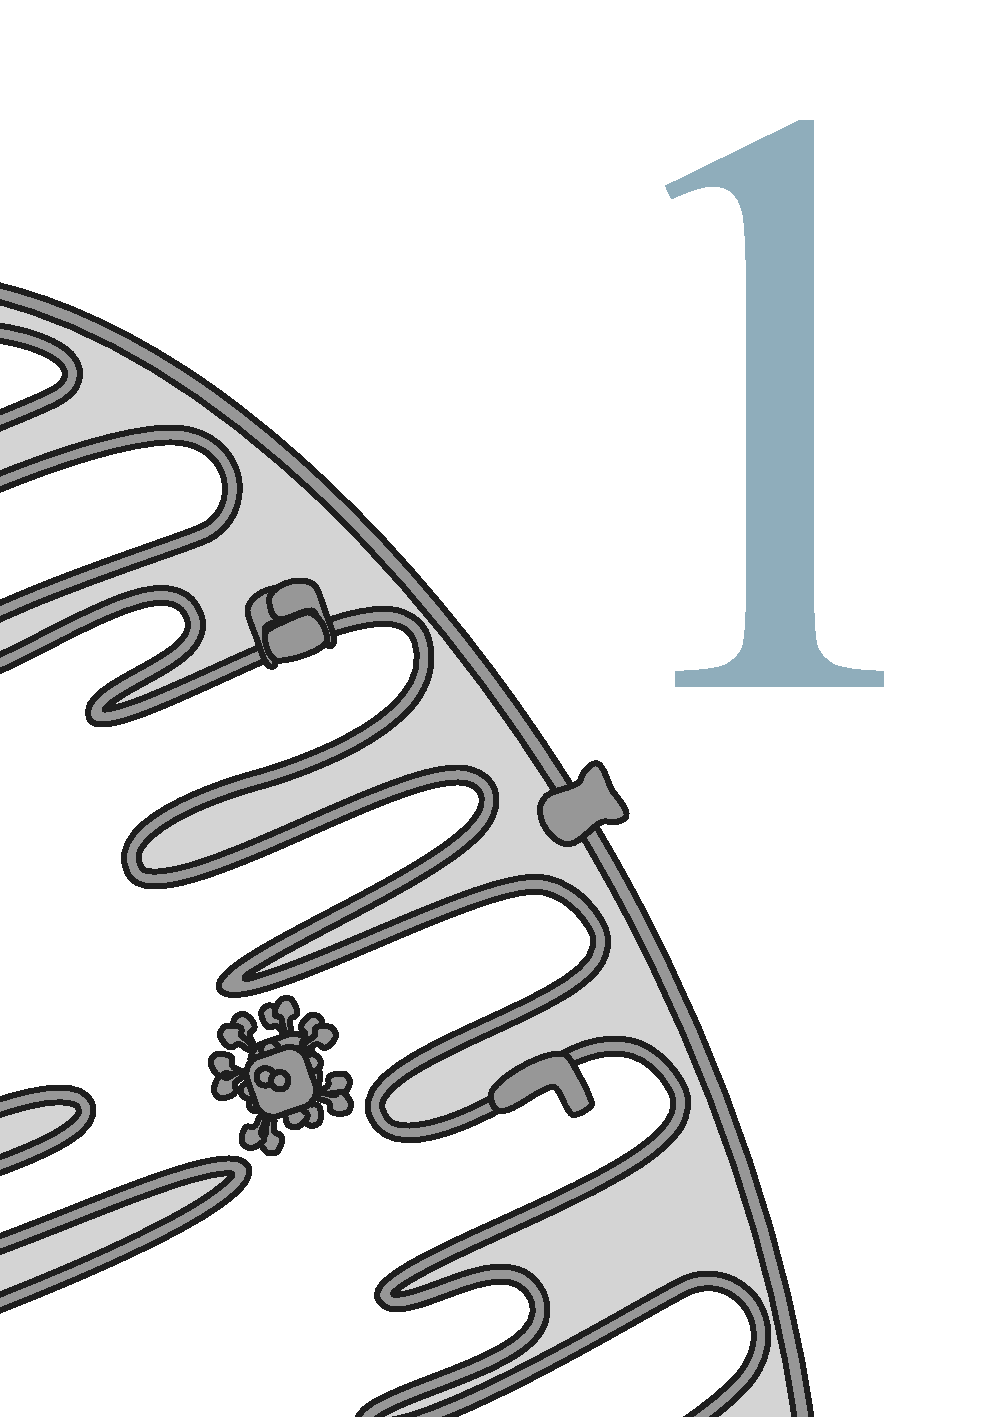
\includepdf{Chapter_covers/chapter_cover_1.pdf} %add Chapter cover on blank page for 1st Chapter
\mainmatter % Begin numeric (1,2,3...) page numbering
\doublespacing % Double spacing
\numberedchapter
%\picturechapterr{Combining cross-linking mass spectrometry and complexome profiling to structurally characterize mitochondrial protein complexes} \label{ch-1}
%
{
    \begin{center}
        \vspace*{4cm}
        \footnotesize
        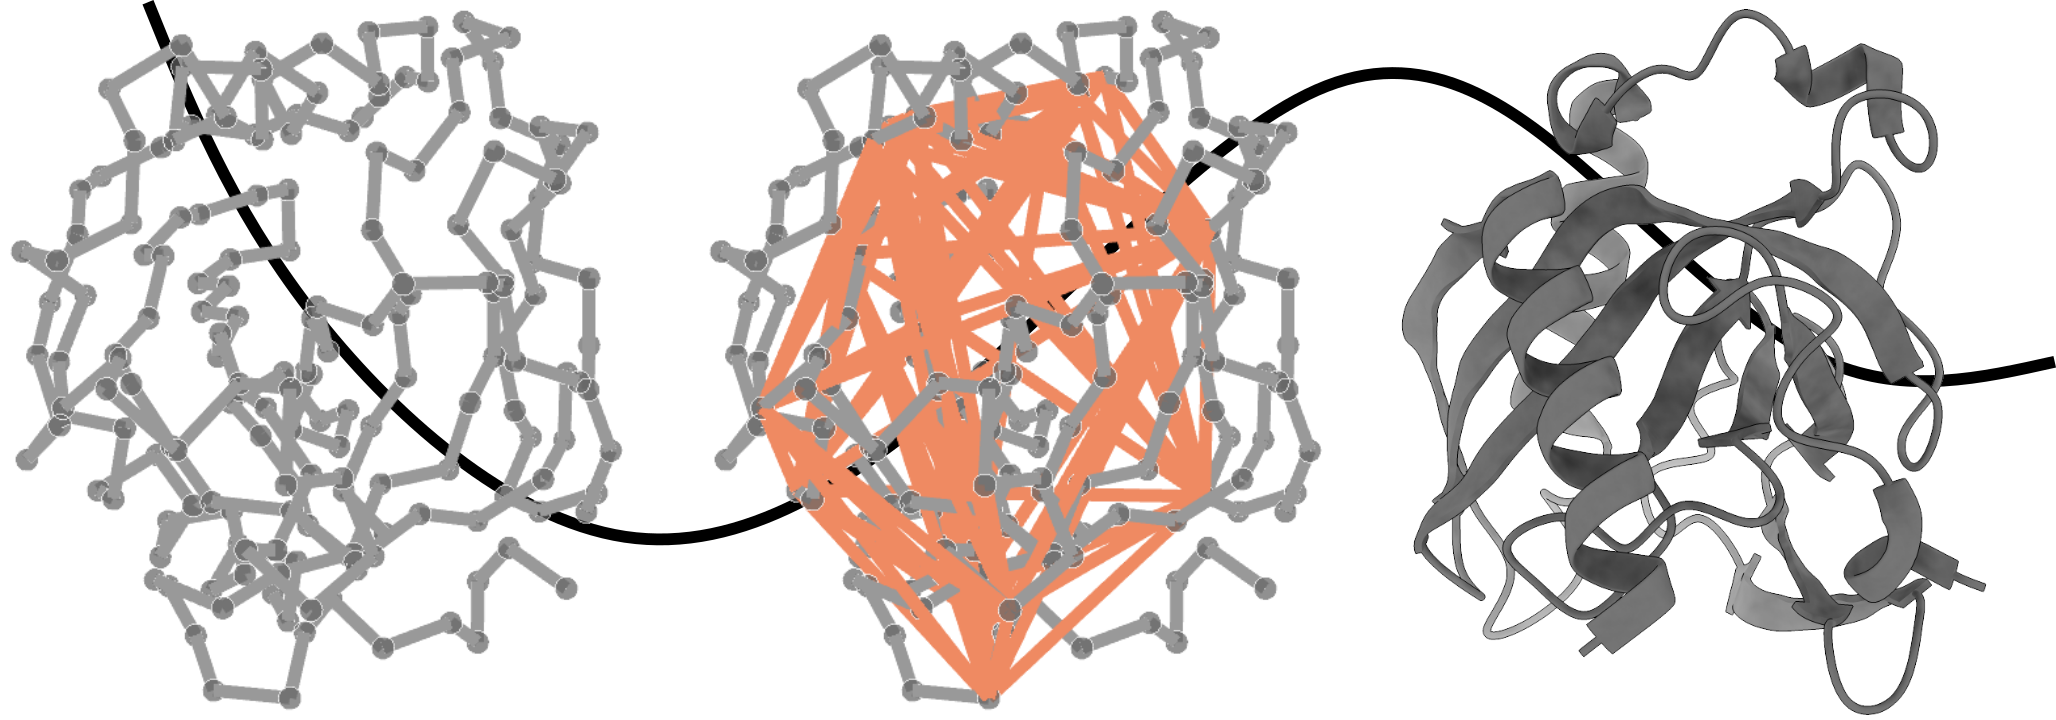
\includegraphics[width=0.6\textwidth]{Chapter.1/Figures/chapter1_cover.png}
    \end{center}
}
%
\begin{flushleft}
    \vspace*{\fill}
    \rule{\textwidth}{1pt}\\[0cm]
    This chapter includes parts of the following publication:\\
    \textbf{Complexome profiling - exploring mitochondrial protein complexes in health and disease}\\
    \footnotesize
    \vspace{0.3cm}
    Alfredo Cabrera-Orefice, Alisa Potter, Felix Evers, Johannes F. Hevler and Sergio Guerrero-Castillo \\
    %\vspace{0.3cm}
    \textbf{\emph{Front Cell Dev Biol.}} (2022), 9:796128, doi: 10.3389/fcell.2021.796128. \emph{Review}\\
\end{flushleft}
\newpage
%
\section{Prelude - The importance of probing protein interactions}
\lettrine[lraise=0.1, nindent=0em, slope=-.5em]{P}{roteins}, the so-called “workhorses” of life, are the tools that make living machines work  \cite{Adams_2008}. The vast majority of biological processes are thus structured, mediated and executed by these macromolecules. Even though many single proteins do perform specific functions by their own, most proteins habitually interact with other proteins, DNA, RNA and lipid molecules rather than acting individually for achieving their biological tasks. The resultant protein complexes can form transient or steady interactions, which also correlate with the type of biological processes they are involved in \cite{De_Las_Rivas_2010}. For example, housekeeping cell processes are likely performed by a large fraction of physically stable protein complexes, whereas in signaling, cell migration, membrane trafficking, metabolic response and other highly dynamic processes, involvement of transient complexes is required for rapid responses and adaptation. The entire set of multi-protein complexes in a cell or compartment is referred to as the complexome \cite{Ceulemans_2006, Deshaies_2002, Lasserre_2006}.

In situations where impaired interaction of the elements of a protein complex affects its proper formation; e.g., due to genetic mutations, the related cell process(es) could be compromised and result in biological dysfunction. Higher complexity in multicellular organisms is of course accompanied by larger complexomes than those from unicellular species. Therefore, alterations in protein complexes may affect not only multiple cell processes, but also lead to severe pathophysiological issues at the tissue/organ level. An integral elucidation of both complexomes and protein interaction networks; i.e., interactome \cite{Vidal_2011} under different cellular scenarios, becomes crucial to fully comprehend the molecular mechanisms behind cell physiology and disease.

Numerous biochemical, biophysical, structural, genetic, microscopy and mass spectrometry (MS) approaches have been applied to characterize protein complexes. Although these methods have different principles, in most cases, they require experimental interventions, cell/tissue fractionation, protein extraction and/or time-consuming protocols prior to data collection and analyses. Besides, the amount of information obtained is often limited to one or a small set of protein complexes. The recent breakthrough in quantitative high-throughput technologies and bioinformatic tools has substantially increased the efficiency and quality of the large-scale identification of protein interactors \cite{Iacobucci_2021, Low_2021}. Accordingly, an outstanding volume of evidence on the composition, 3D structure, interactions and molecular roles of hundreds of protein complexes is now easily accessible through multiple repositories, such as RCSB PDB \cite{Burley_2021}, STRING \cite{Szklarczyk_2021}, CORUM \cite{Giurgiu_2019}, BioGRID \cite{Oughtred_2021}, Pfam \cite{Mistry_2021}, Complex Portal \cite{Meldal_2021}, NCBI \cite{Coordinators_2016} and UniProt \cite{UniProt_2021}. Yet, a substantial fraction of the protein interactors reported in those databases still lack full validation of their occurrence \emph{in vivo} by using novel and more reliable methods.

Further, function and capability to interact is closely linked to a proteins three-dim\-ensional conformation. As such, interrogating structures and interactions of proteins is key to understand cellular processes and therefore has evolved into a significant area of biological research \cite{De_Las_Rivas_2010, Russell_2004}. Discerning structural details of proteins and macromolecular complexes is performed using techniques such as X-ray crystallography, nuclear magnetic resonance (NMR), Small Angle X-ray Scattering (SAXS), cryo-transmission electron microscopy (cryo-EM) as well as cryo-electron tomography (cryo-ET) \cite{Cerofolini_2019, Dunstone_2017}. Especially, X-ray crystallography, NMR and cryo-EM with the ability of providing atomic structures of proteins and protein complexes contributed unprecedented structural and biological insights into processes crucial for cellular life \cite{Cate_1999, Englmeier_2019, O'Connell_2009}. Despite these accomplishments, these more standard techniques also have their limitations. Foremost, they predominantly require a highly purified sample for analysis, consequently proteins and protein complexes are rarely studied in their naïve cellular environment. In recent years it has become very apparent that structures need to be solved \emph{in situ} to fully understand biological processes, but methods enabling \emph{in situ} structural characterization lagged behind \cite{Lucic_2008}. New developments an opposing the reductionist approach, cryo-ET allows to image whole organisms, tissues, cells and organelles. Recorded images are subsequently reconstructed into three-dimensional tomograms, enabling the investigation of macromolecular complexes in a near native environment \cite{Doerr_2017}. Although cryo-ET holds a future potential to image the entire proteome of a cell, it is currently still limited to highly abundant, very large protein complexes such as ribosomes or respiratory chain assemblies \cite{Davies_2014, Turk_2020}. Alternatively, mass spectrometry (MS) allows to study macromolecules and their assemblies independent of their size and abundance and has thereby evolved into a new pillar in the structural characterization of the proteome (structural proteomics). Since the development of electrospray ionization (ESI) \cite{Fenn_1989, Yamashita_1984} and matrix-assisted laser desorption ionization (MALDI) \cite{Karas_1988} in the mid 1980's, rapid technical advancements resulted in a diverse suit of MS-based techniques for the structural characterization of proteins and protein assemblies. A selection of popular structural MS methods is depicted in \textbf{\autoref{fig:fig1}}. The diversity of available methods not only arose from the many different macromolecules present in the proteome but also from different analysis strategies. Fundamentally, MS-based approaches can be divided into protein-centric and peptide-centric strategies \cite{Soldi_2013}. While protein-centric strategies enable the characterization of intact proteins and protein complexes, peptide-centric approaches delineate structural information by enzymatically digesting proteins into peptides prior to MS analysis. Despite those differences, MS based methods can provide highly complementary structural information on proteins and protein complexes such as their conformation, post-translational modifications (PTMs), surface properties, interaction interfaces, stoichiometry and subunit connectivity. Especially in combination with computational modeling, MS based technologies provide a toolbox that is helpful to unravel structural details that would not be easily accessible with other structural approaches.

\begin{figure*}[hbt]
    \center
    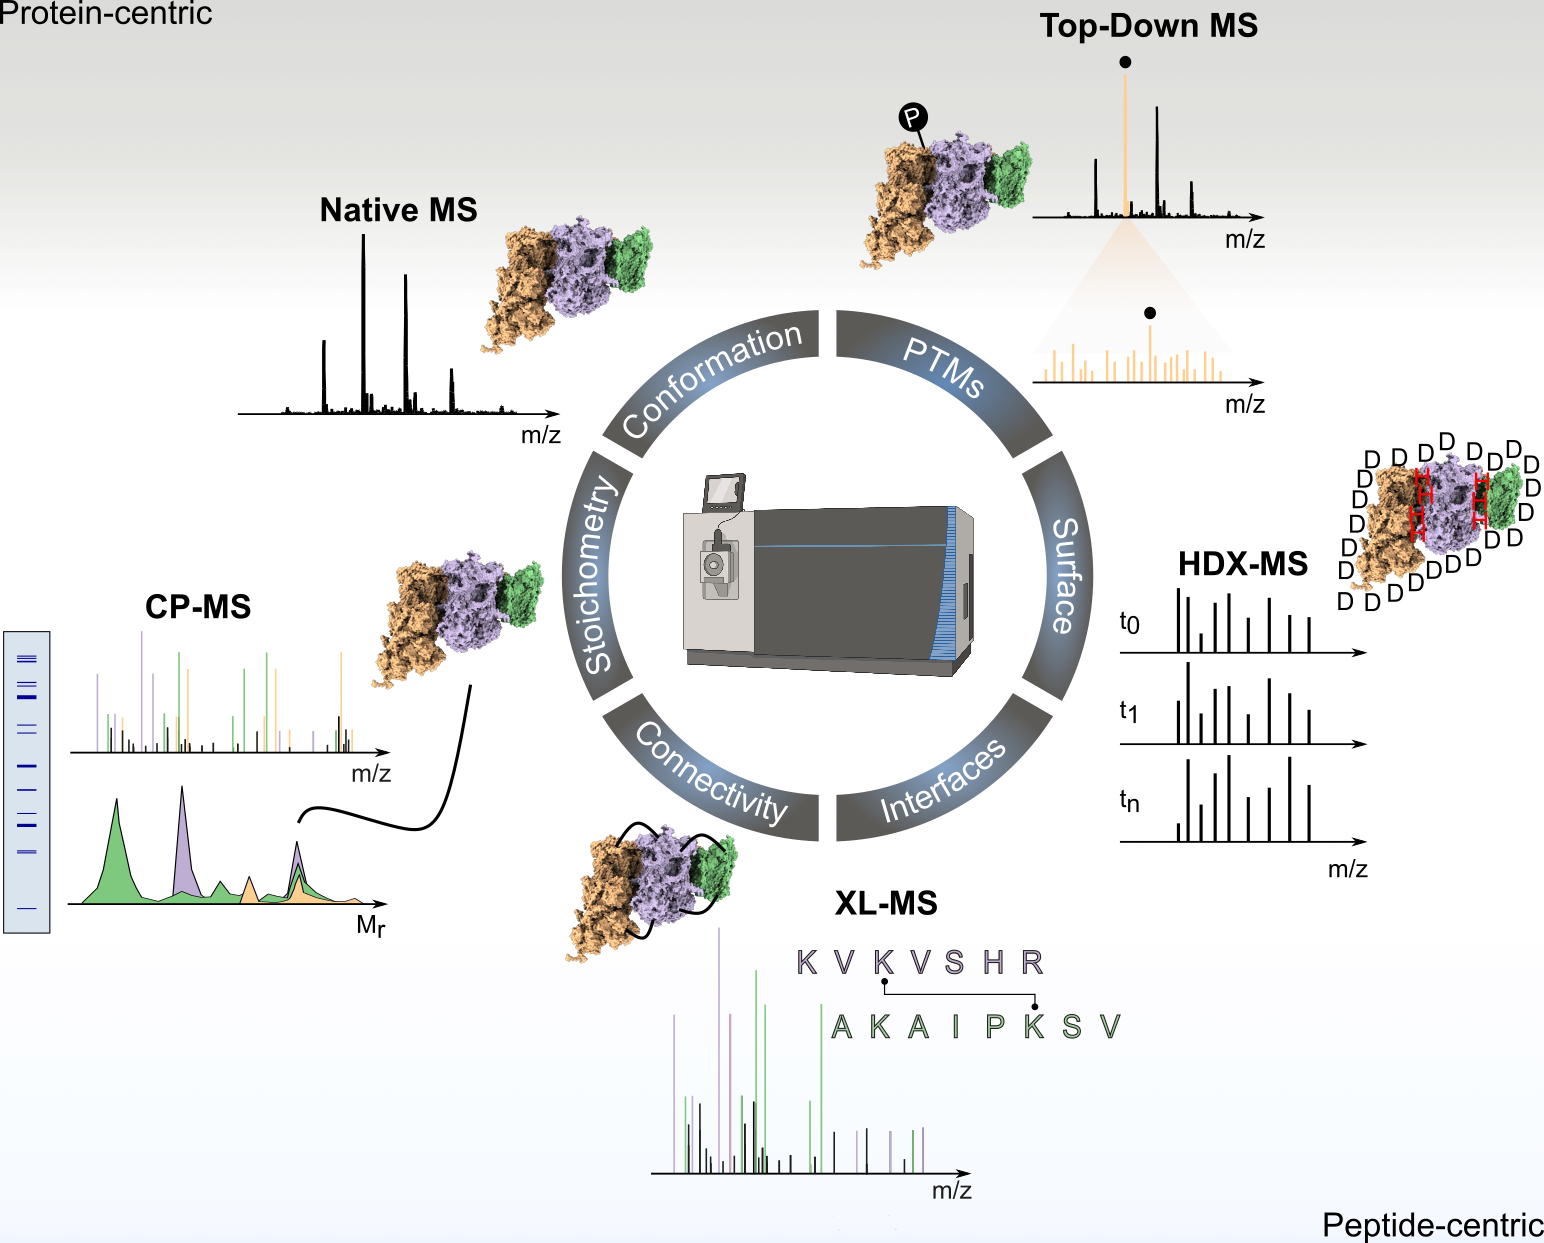
\includegraphics[]{Chapter.1/Figures/Figure1.png}
    \caption{\textbf{Overview of various types of structural MS techniques that can be applied for the characterization of proteins and protein complexes.} The top panel describes protein-centric approaches (native-MS, top-down MS), where intact proteins are analyzed. Complementary, peptide-centric methods (XL-MS, CP-MS, HDX-MS) depicted in the bottom panel, delineate structural information of proteins and protein complexes from peptides.}
    \label{fig:fig1}
\end{figure*} \clearpage
Amongst the versatile MS based toolbox, cross-linking mass-spectrometry (XL-MS) and complexome profiling mass-spectrometry (CP-MS) have emerged as powerful methods to structurally and functionally characterize proteins and protein-protein interactions \cite{Steigenberger_2020}. Nonetheless, both methods also present drawbacks that significantly hamper an adequate structural characterization of protein assemblies. In this thesis I present a collection of XL-MS based advancements that significantly improve the structural and functional analysis of protein complexes in mitochondria. In short, chapter 2 and 3 introduce XL-MS and CP-MS as highly complementary methods, allowing the detailed characterization of protein complexes. Chapter 4 and 5 highlight how XL-MS can aid the identification and characterization of protein complexes using cryo-ET as well as computational structure prediction methods. In the subsequent parts of this introduction, I will succinctly review the fundamentals of XL-MS and CP-MS. The last part will be devoted to how XL-MS in combination with CP-MS and computational modeling, whereby I describe how such a combination can benefit our molecular understanding of mitochondrial protein complexes.
%
\section{The fundamentals of probing protein structure and interactions with XL-MS}
Chemical cross-linking is a special category of protein chemical modifications, and as such it was developed already over 70 years ago to elucidate the chemical and biological function of proteins \cite{French_1945}. Using a cross-linking reagent non-covalent interactions within or between amino acid side-chains of proteins are converted into covalent chemical bonds, stabilizing proteins or protein complexes so that they can be analyzed using methods that normally could denature proteins \cite{Means_1998, Naowarojna_2021}. Like that, cross-linking paired with gel electrophoresis enabled the identification of protein-protein interactions in ribosomes of \emph{Escherichia coli} as early as in the 1970s \cite{Clegg_1974, Sun_1974}. The development of peptide-centric MS methods roughly 30 years later substantially increased the impact of cross-linking for the structural characterization of proteins and respective complexes \cite{Rappsilber_2011, Rappsilber_2000}. Combining cross-linking and peptide-centric MS (XL-MS) enabled not only the fast and sensitive identification of cross-linked proteins but furthermore promised to reveal the position of interacting residues, thereby catering valuable restraints for the structural characterization of proteins and protein complexes. Advances in instrumentation, bioinformatics tools as well as the development of innovative-, MS compatible cross-linkers further increased the application of XL-MS, for instance to study also protein-nucleic acid interactions \cite{Gotze_2021, Wong_1991}.
%
\subsection*{An overview of available cross-linking reagents}
To date, a variety of MS compatible cross-link reagents have been introduced, all aiming at efficiently leveraging spatial distance restraints representative of the in-solution state of proteins and protein complexes. To accomplish this, most of the available reagents typically share a similar structural design, in which two reactive moieties (most commonly amine-reactive) are connected by a spacer arm. However, to account for different applications, e.g. different type of samples as well as to ease the identification cross-linked peptides more elaborated designs have been developed \cite{Steigenberger_2020}. To counteract the low efficiency of the cross-linking reaction, and the subsequent low abundance of cross-linked peptides \cite{Leitner_2014, Leitner_2010}, cross-linkers containing enrichable moieties have been introduced. The usage of linkers with enrichable handles like biotin, phosphonic acid as well as azides proved to significantly increase the number of detected cross-linked peptides, by reducing the huge background of non-modified peptides \cite{Matzinger_2020, Steigenberger_2019, Tan_2016}. Additionally, to simplify the computational challenges that are accompanied with identifying cross-linked peptides, so-called “cleavable” cross-linkers have been introduced. Cleavable-cross-linkers possess a labile moiety between the two reactive groups, which can be cleaved during MS analysis. This reduces the subsequent MS2 sequencing to just a single precursor mass originating from an individual peptide with respective part of the cross-linker attached. In contrast, “non-cleavable” cross-linkers stay intact during MS analysis for which subsequent spectra contain fragment ions of the two linked peptides which significantly hampers the identification \cite{Kao_2011}. A more detailed explanation of MS identification of cleavable and non-cleavable cross-linked peptides will follow below.

\begin{figure*}[hbt]
    \center
    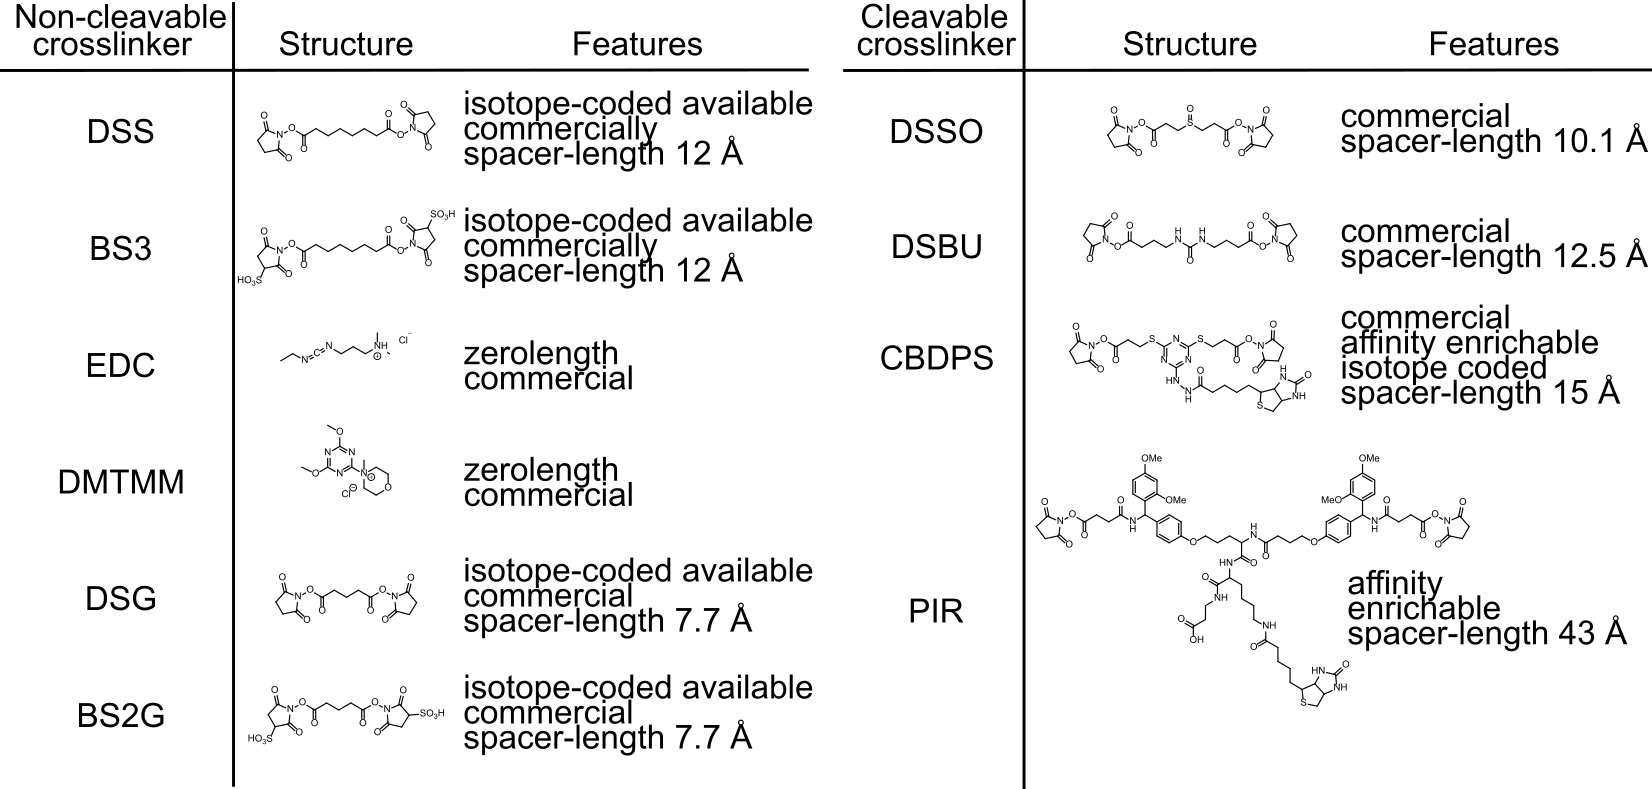
\includegraphics[]{Chapter.1/Figures/Figure2.png}
    \caption{\textbf{Overview of MS-compatible cross-linking reagents.} Figure adapted with permission from \cite{Steigenberger_2020}}
    \label{fig:fig2}
\end{figure*}
Lastly, to further increase the stringency for produced distance restraints, so called “zero-length” cross-linkers have been introduced. These compounds mediate the direct conjunction of two proximal residues with no intervening spacer arm or linker. This theoretically reduces the produced distance restraints to only the length of the side chains ($\sim$15 Å), as opposed to cross-linkers with a spacer arm that produce distance restraints >25 Å. Limiting possible residue-residue distances is especially beneficial when utilized as constraints in computational modelling of proteins or protein complexes, as it reduces the number of possible orientations \cite{Leitner_2014}. An overview of some of the more commonly used cross-linkers is depicted in \textbf{\autoref{fig:fig2}}.
%
\subsection*{XL-MS to characterize protein-protein interactions in mitochondria}
Most cross-linking studies are performed on purified proteins and protein complexes, however in recent years an increasing amount of applications have been reported for more complex systems like whole organelles, cells and even tissue as reviewed in for instance \cite{O'Reilly_2018}. An advantage of working with purified proteins and protein complexes is the significantly simplified detection and identification of cross-links using MS including a more straightforward data analysis. Notwithstanding the challenge, only XL-MS studies of naive systems such as intact mitochondria, can provide a comprehensive interaction network thereby enabling a better understanding of biological processes and dependencies. To tackle the complexity of such systems, several technical and experimental advancements have been presented over the past years enabling the successful identification of mitochondrial protein interactions using XL-MS \cite{Liu_2018, Ryl_2020, Schweppe_2017}.  Given the complexity of mitochondrial proteomes, the selection of a suitable cross-linker, prior to MS-analysis is essential (\textbf{\autoref{fig:fig3}A}). Gas-phase cleavable cross-linkers such as DSSO \cite{Kao_2011} or cross-linkers with an enrichment handle such as PhoX \cite{Steigenberger_2019} significantly simplify the subsequent identification of the XLs. Although NHS- reactive cross-linkers, covalently linking proximal lysine-side chains, are still most commonly applied in cross-linking experiments \cite{Steigenberger_2020}, cross-linkers with an alternative side-chain reactivity are valuable reagents to increase the cross-link coverage. The zero-length cross-linker DMTMM, which promotes the condensation between carboxyl-groups (Glutamic acid, Aspartic acid) and primary amines (Lysines) can increase the cross-linking coverage of membrane proteins, as hydrophobic patches which typically carry none or very few Lysine residues could be targeted via Glutamic acid and Aspartic acid residues \cite{Hevler_2021b}. Importantly, before each application, cross-linking conditions, e.g. the ratio of cross-linker to protein or choosing of a suitable cross-linking buffer, need to be carefully optimized \cite{O'Reilly_2018}. After cross-linking, mitochondria are disrupted either mechanically (e.g. sonication) or by using detergents (e.g. Triton-X-100) and soluble proteins are subsequently denatured, reduced, and alkylated, alike in standard bottom-up proteomics experiments. Before enzymatic digestion of soluble proteins into peptides, contaminations such as lipids and detergents are removed by precipitation or phase extraction \cite{Klykov_2018}. After digestion, cross-linked peptides, which can either stem from the same protein (intra cross-link) or from two distinct proteins (inter cross-link), are significantly less abundant than their “linear” (non cross-linked) and “mono-linked” counterparts \cite{Leitner_2014, Leitner_2010, Sinnott_2020} (\textbf{\autoref{fig:fig3}B}). Mono-linked peptides are linear peptides which carry the cross-linker that is quenched or hydrolyzed on the other reactive group rather than attached to another peptide. In contrast to linear peptides, mono-linked peptides contain structural information and are commonly used to assess protein surface accessibility as well as to support scoring of structural models \cite{Sinnott_2020}. The sub-stoichiometric reaction efficiencies render the identification of cross-linked peptides challenging, especially in complex samples such as intact cell and mitochondria. To obtain satisfactory identification of cross-linked peptides relative to their linear counter parts, an enrichment step is often essential (\textbf{\autoref{fig:fig3}C}). Enrichment most often takes place via chromatographic methods, such as strong-cation-exchange (SCX) fractionation, that can be used to separate doubly charged linear (tryptic) peptides (carrying a charge at the N and C terminus) from higher charged, cross-linked peptides (typically carrying double the number of charges). In case an enrichment handle such as a phosphonate group (PhoX) is used, cross-linked peptides can be captured onto a suitable material (e.g. Fe3+ IMAC), thereby allowing the separation from linear peptides. After enrichment, cross-linked peptides are identified following different MS acquisition strategies (\textbf{\autoref{fig:fig3}D}). Which MS acquisition method to use, is largely determined by the applied cross-linker \cite{Liu_2017a}. Lastly, recorded XL-MS spectra can be searched using various software suits
\begin{figure*}[p]
    \center
    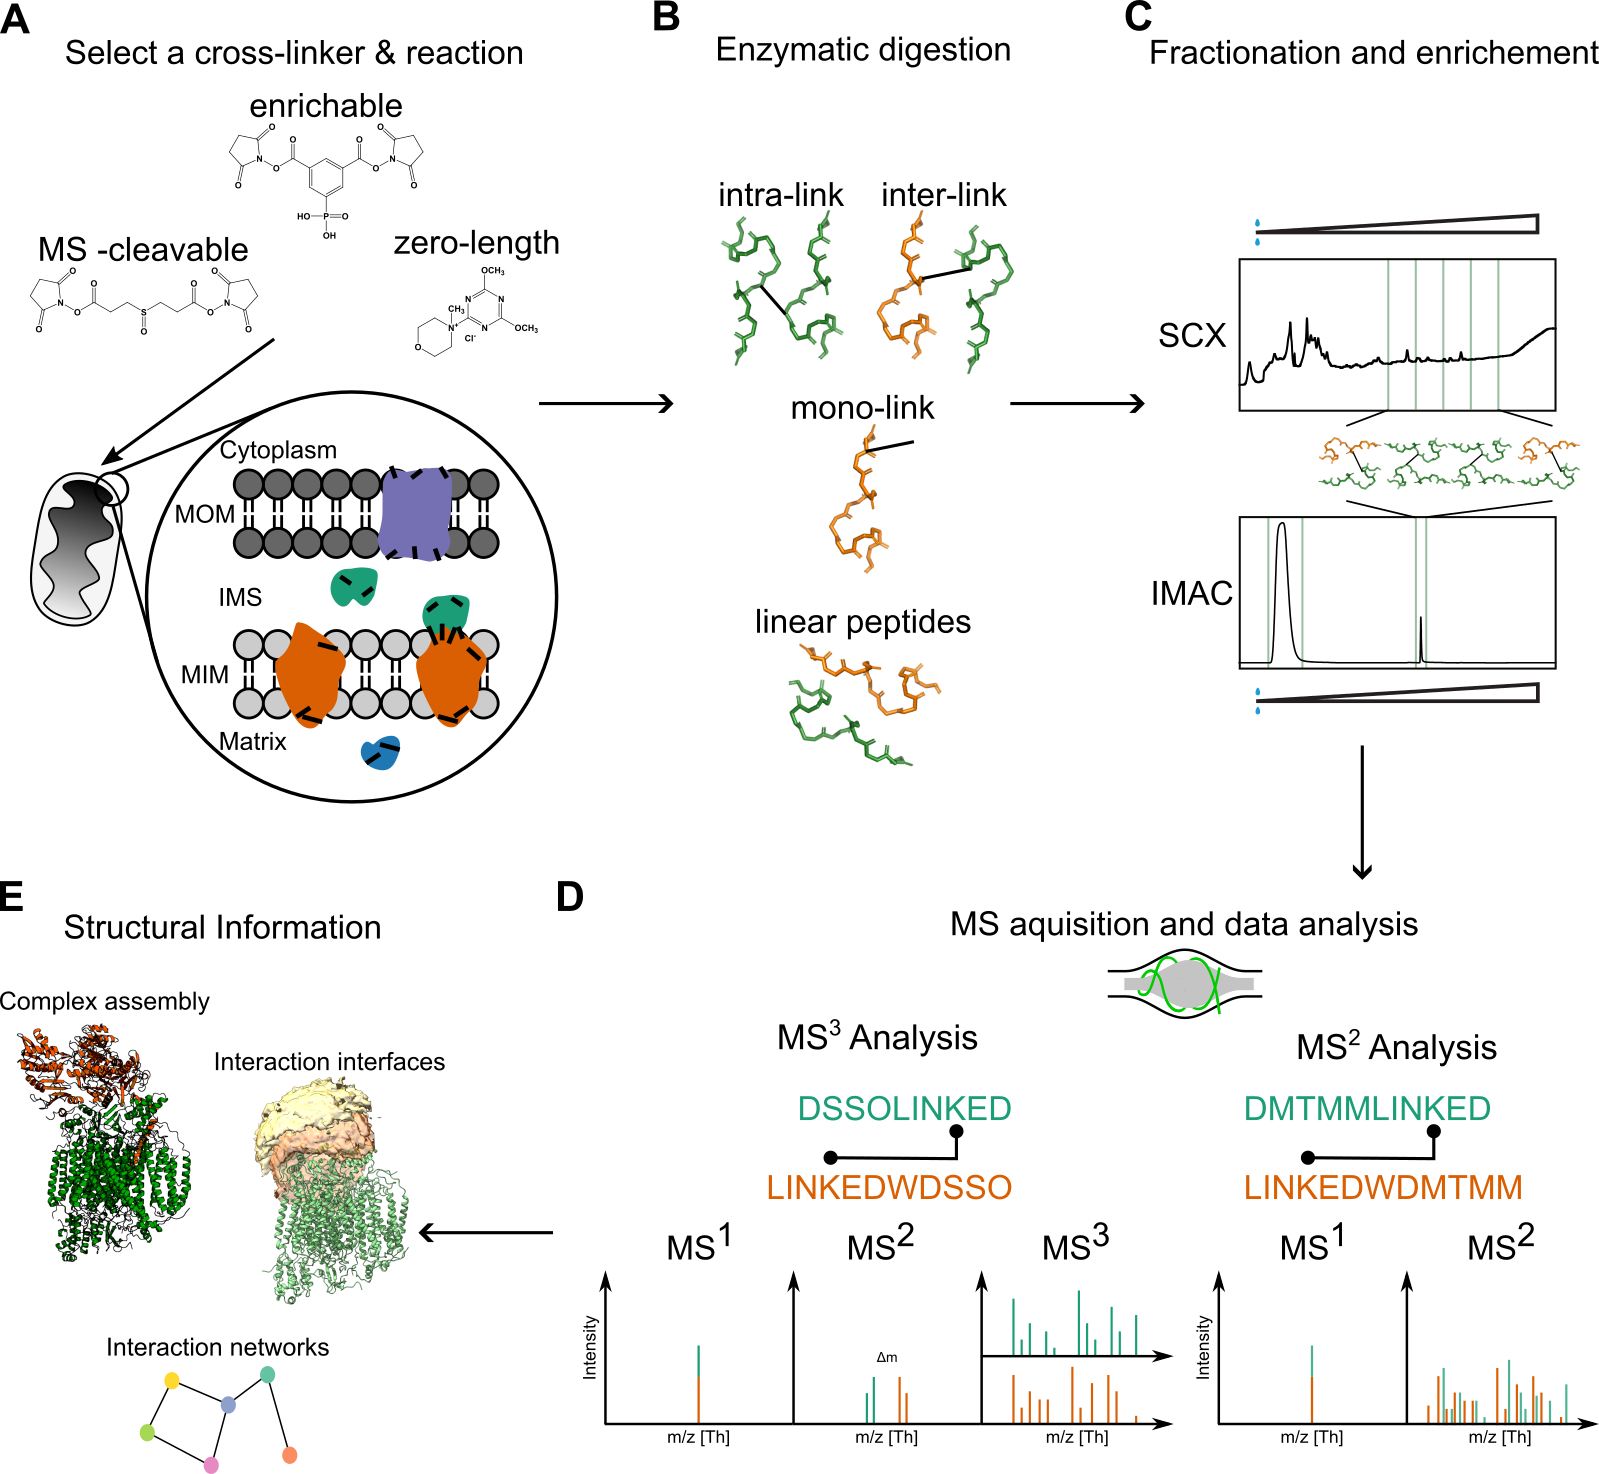
\includegraphics[width=0.95 \textwidth]{Chapter.1/Figures/Figure3.png}
    \caption{\textbf{Experimental strategies for the analysis of proteome-wide protein-protein interactions in mitochondria.} \textbf{A.} Cross-link reagents comprise various chemistries as highlighted in \textbf{\autoref{fig:fig2}}. For cross-linking mitochondria, reagents with a cleavable spacer arm, enrichable handle or an alternative amino-acid reactivity are beneficial to increase the number of cross-link identifications. DSSO is depicted here as an example for a cleavable cross-linker. PhoX is depicted as an example for a cross-linker with an enrichment handle (phosphonic acid) and DMTMM is depicted as example for a zero-length cross-linker. For each application, conditions such as concentration and reaction time need to be carefully optimized to achieve optimal cross-linking. \textbf{B.} After solubilization of mitochondrial membranes proteins are enzymatically digested, producing a mixture of cross-linked and linear peptides. Cross-links can be formed within protein sidechains (intra link) and between sidechains of different proteins (inter link). Additionally, linear peptides with the cross-linker attached (mono-links) can be formed. \textbf{C.} To increase MS identification, cross-linked peptides are separated from linear peptides using chromatographic methods, such as strong-cation-exchange chromatography (SCX) or Fe3+ IMAC enrichment chromatography. \textbf{D.} Depending on the chosen cross-linker (e.g. gas-phase cleavable or non-cleavable) different MS acquisition strategies can be applied, to increase the likelihood of identifying a cross-linked peptide. \textbf{E.} Different software solutions as described in the text can be utilized to identify linked peptides. Information of cross-linked experiments can be used to elucidate protein-protein networks, interaction interfaces as well as to structurally model protein complex assemblies as described in the text. Figure adapted from \cite{Hevler_2021b}.}
    \label{fig:fig3}
\end{figure*}
such as pLink2 \cite{Chen_2019b}, MeroX \cite{Gotze_2015}, StavroX \cite{Gotze_2012}, Xi \cite{Chen_2019a}, Kojak \cite{Hoopmann_2015} and XlinkX \cite{Klykov_2018}. However, not all software solutions are capable of analyzing all MS-acquisition strategies or cross-link reagents (e.g. MS3, DSSO), as such software capability as well as availability should be taken into consideration when designing a XL-MS experiment. Likewise, methods for FDR calculations might differ across platforms, thereby impacting the quality and ambiguity of outputted XL-MS results \cite{Matzinger_2022}. Careful manual validation of identified cross-linked peptides is still advisable before utilizing them for the structural characterization of protein complexes (\textbf{\autoref{fig:fig3}E}). Strategies for MS-acquisition, and applications of XL-MS for structural characterization of proteins and protein complexes will be further discussed in the following sections.
%
\subsection*{XL-MS-data acquisition}
In classical bottom-up proteomics, linear peptides are identified based on their accurate mass (measured at the MS1 level) and sequence specific fragment ions (measured at the MS2 level). To be analyzed within the mass spectrometer, peptides are first ionized and thereby separated from their carrier medium (usually aqueous or organic phase). Charged and ionized peptides are next transmitted into the mass spectrometer, where the mass of the intact peptide-ion is determined by a mass analyzer (MS1 signal). The mass of each ion is measured by monitoring their motion through the mass analyzer, which is dependent on the mass to charge ratio (m/z). Work presented in this thesis utilized instruments equipped with quadrupoles, linear ion traps (LIT) as well as an Orbitraps as mass analyzers. To confidently determine the correct peptide sequence, the peptide ion is fragmented inside the mass spectrometer providing additionally m/z values for its fragment ions (MS2 level). Depending on the fragmentation technique used, different fragment ions corresponding to cleavage of the peptide backbone can be observed. Most frequently, collision-induced dissociation (CID) \cite{Hunt_1986} and higher-energy C-trap dissociation (HCD) \cite{Olsen_2007} fragmentation techniques are applied, producing b and y fragment ions that reflect N- and C-terminal fragments, respectively being cleaved at the peptide bonds. For XL-MS applications, further fragmentation of an isolated fragment ion (MS3 level) can be very useful, however not all mass spectrometers are capable of performing such higher order, e.g. MS3, experiments \cite{Liu_2017a, Lossl_2016}.\\
For XL-MS experiments, the seemingly well-established MS analysis for the identification of linear tryptic peptides is substantially impaired, due to the fact that the cross-linked peptide is composed of two covalently bound linear peptides. As such, the two peptide moieties presents in these cross-linked peptide precursor ions are normally co-fragmented in the same MS2 spectra, often with different fragmentation efficiencies for the two peptide moieties hampering the full identification of both \cite{Liu_2017a}. To circumvent impaired fragmentation and to increase the fragmentation efficiency, cross-linked peptides are commonly fragmented using multiple collision energies (CID/HCD), resulting in more informative fragmentation spectra (MS2 method). Importantly, also the cross-link reagent moiety can impact the fragmentation. Consequently, collision energies need to be optimized for each cross-linker to obtain the best fragmentation efficiency. Likewise, combining complementary dissociation methods such as CID/HCD and electron transfer dissociation (ETD) can be applied for an improved fragmentation (MS2-MS2 method) \cite{Campbell_2009, Frese_2012, Liu_2017b} (see \textbf{\autoref{fig:fig3}D}). Additionally, gas-phase cleavable cross-linkers \cite{Sinz_2017}, such as DSSO have been developed to address such impaired fragmentation. Such cross-linkers are cleaved during the fragmentation process of the XL peptide ions inside the vacuum of the mass analyzer, thereby enabling the dissociation of the cross-linked peptides and greatly improving fragmentation and thus cross-link identification of the two peptide moieties \cite{Liu_2017a}. When measuring on mass spectrometers capable of MS3 analysis, a dual-fragmentation strategy for cleavable cross-linkers can be applied. In such an approach, a survey scan (MS2) is performed, in which a dissociation energy is chosen that specifically breaks the cleavable cross-linker thereby giving rise to signature ions with a unique mass difference corresponding to the cleaved cross-linked peptide each with a part of the cross-link moiety attached. Whenever the mass spectrometer identifies the XL-peptide signature ions, a subsequent isolation and fragmentation step is performed to obtain better sequence information (MS3 analysis) \cite{Liu_2017a, Sinz_2017} (see \textbf{\autoref{fig:fig3}D}). The utilization of gas-phase cleavable cross-linkers in combination with MS3 acquisition strategy has been found to be extremely useful for the analysis of proteome-wide XL-MS experiments such as cell lysates \cite{Klykov_2018, Liu_2017a} as well as intact organelles such as mitochondria \cite{Liu_2018} or nuclei \cite{Fasci_2018}. Notwithstanding, it was recently shown that MS2- and MS2-MS2 acquisition methods can outperform MS3 acquisition strategies in terms of unique crosslink numbers \cite{Matzinger_2022}, suggesting that the new generation of MS2 capable mass-spectrometers can also be used for analysis of proteome-wide, gas-phase cleavable XL-MS experiments.
%
\subsection*{Applications of XL-MS for the structural characterization of protein complexes}
Beyond what is well possible using more common techniques in structural biology, XL-MS can also be performed under naïve cellular conditions, reducing possible artifacts that may occur during recombinant expression and/or purification of proteins and protein complexes \cite{Niedzialkowska_2016}. In the latter case additional artefacts may occur during in vitro reconstitution of a protein complex. Additionally, benefits of probing protein-protein interactions \emph{in vivo} have been shown in work on mouse heart mitochondria, for which a number of protein-protein interactions could only be observed in intact mitochondria and not upon membrane disruption \cite{Liu_2018}. XL-MS studies applied to cell lysates or intact organelles such as mitochondria, have successfully captured proteome-wide PPIs, thereby enhancing our understanding of how the proteome is wired \cite{Fasci_2018, Klykov_2018, Liu_2017b, Ryl_2020, Schweppe_2017} (\textbf{\autoref{fig:fig4}A}). While such interaction networks are also commonly generated through other MS based methods such as affinity-purification MS (AP-MS) \cite{Huttlin_2017, Krogan_2006}, intra and inter cross-links generated by XL-MS additionally provide information that can be used for the structural characterization of proteins and protein complexes \cite{Bullock_2018, Klykov_2018, Orban-Nemeth_2018}. Intra protein cross-links provide information about proximal amino acids within a protein, which can be applied as distance restraints in subsequent computational modeling \cite{Orban-Nemeth_2018} (\textbf{\autoref{fig:fig4}B}). Distances for cross-link restraints applied in computational modeling are mostly calculated between C\(\alpha\)-C\(\alpha\), by summing the length of each side chain and the length of the cross-linker. As side-chains and cross-linkers are highly flexible, distance restraints are typically provided as a range (with a minimum and maximum value) rather than a defined distance value. Modeling software`s such as I-Tasser \cite{Yang_2015}, Robetta \cite{Kim_2004} and Modeller \cite{Webb_2016} employ set cross-link constraints for model building as well as for scoring features (e.g. geometry) of the structure which may not be evaluated by standardly used score terms. Recent breakthroughs in the field of protein structure prediction by AI driven tools such as AlphaFold2 \cite{Jumper_2021} and RoseTTA-fold \cite{Baek_2021}, enable the generation of structural models based solely on the amino acids sequence of a protein. However, validation and finding the biological relevant confirmation can be time consuming and challenging with only having the provided output scores at hand. For this, it was recently shown that intra cross-links can be utilized to aid the validation process as well as to pinpoint towards biologically active structural conformations \cite{McCafferty_2022}.

Moreover, \emph{ab initio} protein-protein docking offers a possibility to computationally predict protein complexes and protein-protein interfaces, given that the structures of the individual sub-units are known \cite{Dominguez_2003, Vakser_2014}. For most of the available programs complex
conformations are predicted by rotating and translating one complex component (often the smaller protein) around the other one, which is fixed in space.

\begin{figure*}[htb]
    \center
    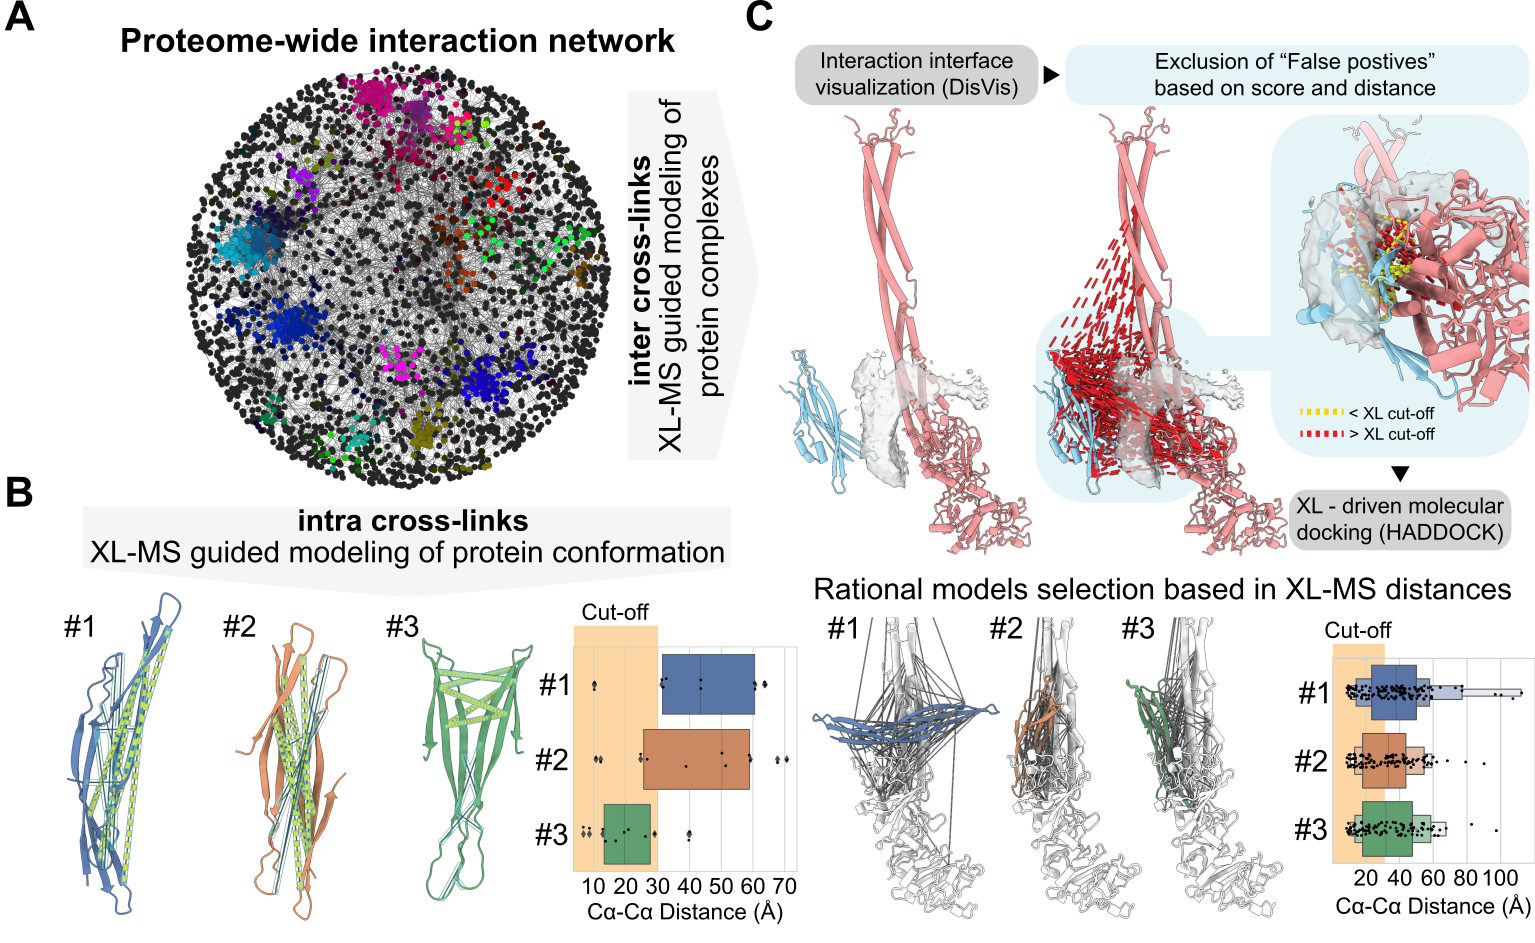
\includegraphics[]{Chapter.1/Figures/Figure4.png}
    \caption{\textbf{Applications of XL-MS for the structural characterization of proteins and protein complexes} \textbf{A.} When XL-MS is applied on high complex samples, such as cell lysates or intact organelles, protein-protein interaction networks can be generated. Protein interaction networks highlight how a soluble proteome is wired. Proteins are shown as black nodes, with proteins that have a similar GO functional annotations \cite{Ashburner_2000} being depicted in bright colors. \textbf{B.} Intra protein cross-links can be utilized to guide structural modeling of a protein conformations, as well as to validate AI derived structural models. \textbf{C.} Inter protein cross-links can be utilized to model protein complexes observed in the interaction network. Information about proximal amino acids is validated and utilized to identify interaction interfaces and active interface residues (e.g. using DisVis \cite{van_Zundert_2015}). True positive inter-crosslinks as well as information about active interface residues can subsequently be used as input for protein-protein docking (e.g. using Haddock \cite{van_Zundert_2016}). Validation of generated complex models can be performed by mapping obtained inter cross-links onto final structures. Figure adapted from \cite{Lagerwaard_2022} with permission. Data to generate the protein-protein interaction network was obtained from \cite{Costanzo_2016}}
    \label{fig:fig4}
\end{figure*}\clearpage
This approach, however, is still very time consuming and computationally expensive as all theoretically possible conformational spaces have to be sampled and scored \cite{Dominguez_2003, van_Zundert_2016}. Inter protein cross-links identified in XL-MS experiments, provide information about the arrangement of proteins within a complex. Utilizing inter cross-links as additional restraints to guide the docking process alongside traditional energetics and shape complementarity can therefore significantly reduce the possible conformational space and increase the chance for the prediction to result in a unique solution \cite{Dominguez_2003, van_Zundert_2016} (\textbf{\autoref{fig:fig4}C}). HADDOCK \cite{Dominguez_2003, Orban-Nemeth_2018} (High Ambiguity Driven protein-protein Docking) is a powerful tool that can make use of biochemical and/or biophysical interaction data such as inter cross-links observed in XL-MS experiments. To utilize cross-links for guiding structural docking, the provided information content needs to be first evaluated. DisVis \cite{van_Zundert_2015} is a software suit enabling the identification of false-positive cross-links as well as the characterization of surface residues that are most often contacted in all possible models (interface residues). True-positive cross-links together with active interface residues are employed as additional restraints to predict a protein complex and later for validation and model selection. Besides guiding protein-protein docking, cross-linking data was shown to benefit other structural and modeling techniques, for instance with the assignment of ambiguous densities in cryo-EM maps \cite{Herzog_2012, Kyrilis_2021b} or with identifying and refining high confidence models predicted for protein complexes based on AI \cite{Burke_2021}.

Although the prime technology used for the work described in this thesis is cross-linking mass spectrometry, several of the chapters involved the use of another powerful approach, namely complexome profiling. Below I describe succinctly also this approach, largely adapted from \cite{Cabrera-Orefice_2022}, and include a description of some of the more recent applications of this method especially looking into mitochondrial protein complexes in all the kingdoms of life.
%
\section{The fundamentals of characterizing protein complexes with complexome profiling mass spectrometry (CP-MS)} \label{sec:CP_MS_intro}
The first requisite to carry out a complexome profiling (CP) experiment is the collection of biological material; e.g. tissue pieces/biopsies, cultured cells, enriched cell fractions, purified organelles, etc. These materials might also come from previous experimental interventions. Homogenization and cell fractionation methods should aim to keep the native state of protein complexes. For solubilization of membrane proteins, it is recommended to use mild, non-ionic detergents; e.g., Triton X-100, NP-40, dodecyl-maltoside, octyl-glucoside or digitonin \cite{Eubel_2005, Wittig_2006}. Next, native protein extracts are separated by a so-called “untargeted” method \cite{Iacobucci_2021}, such as native electrophoresis, size-exclusion chromatography or density gradient ultracentrifugation (\textbf{\autoref{fig:fig5}}). Regardless of the type of protein separation, CP follows a well-defined protocol that slightly differs among variants. In all cases, protein complexes are separated by size, hence, by shape and molecular mass. Each fraction is further digested with high-purity and specific proteases (e.g., trypsin, chymotrypsin and endoproteinase Lys-C) followed by MS/MS identification of the resulting peptides \textbf{\autoref{fig:fig5}}; i.e., bottom-up proteomics strategy \cite{Zhang_2013}.\\
Prior to MS analysis, peptides are usually separated based on their hydrophobicity by reversed-phase high-performance liquid chromatography (RP-HPLC) followed by electrospray ionization (ESI) to produce gas phase ions \cite{Zhang_2013}. The majority of MS data for CP studies has been acquired in data-dependent mode (DDA); i.e. collection of a predefined number of precursor ions for fragmentation during the MS2 cycle is done according to their charge states and abundance \cite{Hu_2016}. In conventional DDA modes, the possibility to identify low abundant peptides thus becomes significantly limited. To avoid this issue, acquisition strategies in data-independent mode (DIA) \cite{Krasny_2021}, such as sequential window acquisition of all theoretical mass spectra (SWATH-MS) \cite{Gillet_2012}, in which fragmentation of all precursor ions identified in the MS1 cycle can be analyzed in the MS2 cycle, have recently been introduced to CP-like workflows \cite{Bludau_2020, Calvo_2020, Heusel_2019}.

MS spectra are routinely matched against a proteome database of the species of interest by using a variety of software/search engines (\textbf{\autoref{fig:fig5}}), such as Mascot \cite{Perkins_1999}, openMS \cite{Rost_2016}, PEAKS DB \cite{Zhang_2012}, Proteome discoverer \cite{Orsburn_2021}, Protein Prospector \cite{Chalkley_2005} and MaxQuant \cite{Tyanova_2016a}. In case that the proteome of the studied organism is not yet available or fully annotated, metagenome or transcriptome data are useful to generate a list of proteins and perform the search. Alternatively, peptide sequences might be deduced directly from tandem MS spectra by using database-independent computational approaches; i.e. \emph{de novo} peptide sequencing \cite{Tran_2017}.

Protein abundance profiles are further obtained by plotting, for example, label-free quantification (LFQ) \cite{Cox_2014} or intensity-based absolute quantification (iBAQ) \cite{Schwanhausser_2011, Tyanova_2016a} values over each of the collected fractions. While LFQ intensities are typically utilized for comparing relative amounts of proteins in multiple samples, iBAQ values offer a more stoichiometric impression of the identified protein groups as those are proportional to their molar quantities. iBAQ values are calculated as the sum of all individual peptide intensities of a given protein group divided by its number of theoretical identifiable peptides. It is thus not surprising that the majority of CP studies use iBAQ since it enables a more fair comparison between different protein groups in the same and multiple samples. Additional information regarding LFQ and other alternative methods have been reviewed in \cite{Fabre_2014, Wittig_2021}. Ultimately, the list of hundreds or even thousands of identified proteins is mainly sorted based on similarities of the abundance patterns across fractions by hierarchical clustering analysis (\textbf{\autoref{fig:fig5}}). \clearpage
\begin{figure*}[hb!]
    \center
    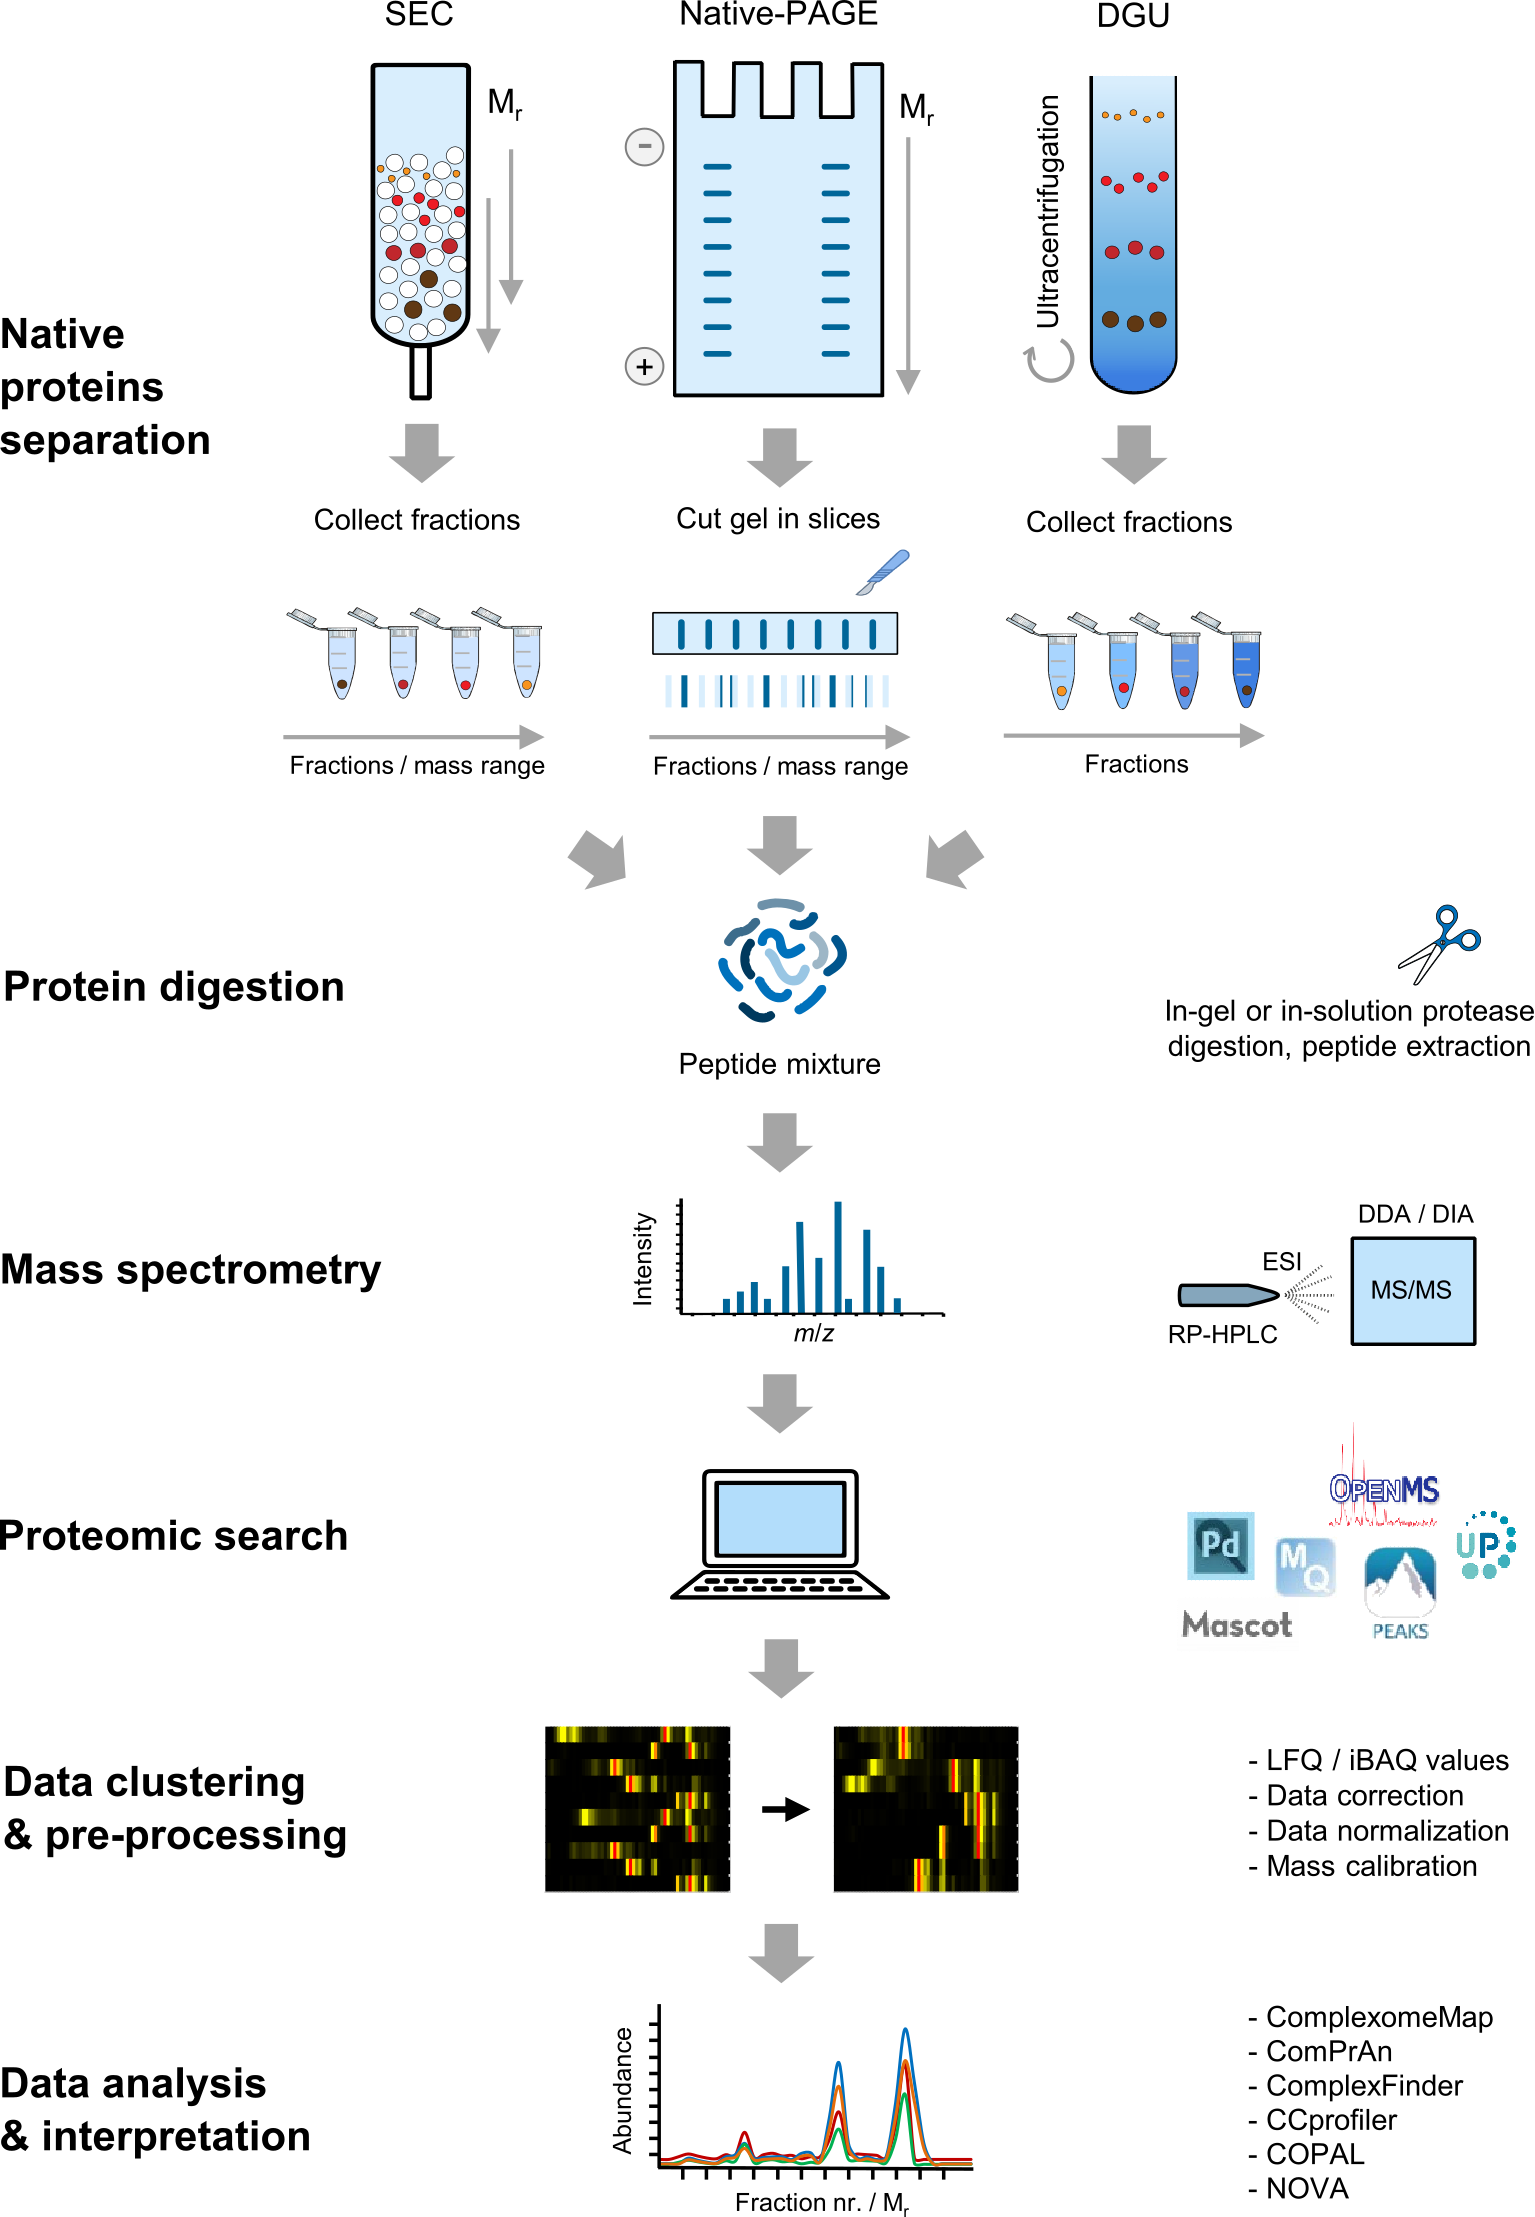
\includegraphics[width=0.9 \textwidth]{Chapter.1/Figures/Figure5.png}
    \caption{Figure Legend on next page}
    \label{fig:fig5}
\end{figure*}
\addtocounter{figure}{-1}
\begin{figure*}[ht!]
    \caption{\textbf{Overall workflow of complexome profiling (CP).} After collection, homogenization and fractionation of biological materials, proteins are separated by either native polyacrylamide gel electrophoresis (PAGE), size exclusion chromatography (SEC) or density gradient ultracentrifugation (DGU) for CP studies. The obtained protein-containing fractions are individually digested with specific proteases. Resultant peptides are extracted, cleaned and usually separated by reversed-phase high-performance liquid chromatography (RP-HPLC) followed by tandem mass spectrometry (MS/MS) analysis. MS data can be acquired in data-dependent or data-independent modes, DDA or DIA, respectively. Next, a proteomic search is performed to match obtained MS spectra against proteome databases using a variety of available software. Icons of the most popular tools used for CP studies are shown (see \textbf{\autoref{sec:CP_MS_intro}}). Protein abundance profiles are further obtained by plotting LFQ/iBAQ values against the number of fractions. The list of identified protein groups is computationally sorted based on similarities of the abundance patterns across fractions; e.g. hierarchical clustering. Prior to analysis, complexome data are pre-processed to account for protein loading/MS sensitivity differences. Data correction and normalization between samples are regularly applied. In SEC- and native-PAGE-based CP, a mass calibration can be implemented for a more meaningful biological dimension. Data can be analyzed by using available bioinformatic tools specifically created for CP (see \textbf{\autoref{ssec:CP_MS_ssec2}}). Some of these programs are shown in the figure. Figure adapted from \cite{Cabrera-Orefice_2022}.}
\end{figure*}
Proteins that are part of the same complex consistently cluster together since these show co-migration in the same fraction(s) and similar abundance profiles.
%
\subsection*{Different complexome profiling set-ups, one common goal}\label{ssec:CP_MS_ssec1}
As a ground-breaking “-omics” method, CP has been rapidly developing and spreading among the scientific community. It is thus not striking that in less than a decade, multiple strategies have complemented or even improved its scope. At the same time, several limitations of CP have been circumvented gradually by including novel MS-based strategies, specific adaptions in sample processing and new tools for data analysis. All variants of CP do share a common goal nonetheless: to unravel the composition of protein complexes, as well as their abundance, stabilities, apparent molecular masses and stoichiometries.\\
The most used CP workflow, currently referred to as “classic CP” \cite{Wittig_2021}, uses Blue Native-polyacrylamide gel electrophoresis (BN-PAGE) followed by MS identification. The main advantages of BN-PAGE are the relatively low amounts of biological material required and high-resolution separation of native proteins. BN-PAGE conditions keep proteins in similar native states to those occurring \emph{in vivo} \cite{Wittig_2006}. However, if the presence of Coomassie blue dye affects the stability of one or more protein complexes of interest, milder dye-free versions of native-PAGE can easily be used instead; e.g., high-resolution clear native-PAGE (hrCN-PAGE) \cite{Ladig_2011, Wittig_2007}. Native-PAGE is suitable for separation of proteins between $\sim$0.02-10 MDa. If the study requires interrogation of bigger protein complexes (>10 MDa), large pore BN-PAGE (LP-BN-PAGE) can be applied instead \cite{Heide_2012, Strecker_2010}.

After electrophoresis, entire gel strips are fixed and often cut into 32-70 slices followed by LC-MS/MS identification \cite{Giese_2021, Heide_2012, Senkler_2017, Vidoni_2017}. For CP analysis, slice numbers can be transformed into apparent molecular mass values by carrying out a calibration using standard proteins as exemplified in \cite{Heide_2012, Wittig_2010}. Molecular mass accuracy is optimized by using different sets of standard protein complexes, one for water-soluble proteins and the other for membrane proteins. On the whole, the more fractions collected the better resolution of the resultant profiles will be. In 2016, Müller and co-workers developed cryo-slicing Blue Native-Mass Spectrometry (csBN-MS), which helped increase the resolution, accuracy and quantification of the complexome profiles by slicing the BN-lanes in 230 pieces as well as optimizing MS analysis and protein identification \cite{Muller_2016}. The resolution of complexome profiles obtained from \(\leq\) 30 slices would not be suitable to unambiguously assign protein interactions.

Besides native-PAGE, size exclusion chromatography (SEC) and density gradient ultracentrifugation (DGU) have been implemented in different CP setups. Using SEC, native proteins are separated by filtration through a gel matrix (resin), which consists of spherical porous beads of different sizes depending on the desired range of molecular masses \cite{Burgess_2018}. Elution of heavier proteins is faster than the lighter ones by this method. Apparent molecular masses of eluted fractions can be determined with proper standard mixes; although the mass calibration is more accurate for globular proteins \cite{Hong_2012, Korepanova_2012}. SEC resins are suitable for separating proteins in a wide range of molecular masses; e.g. 1-700 kDa (SephadexTM, SuperdexTM); 5-5000 kDa (SuperoseTM) and 0.01-40 MDa (SepharoseTM). The number of fractions that can be collected after SEC is comparable to those aforementioned. For example, in the recently introduced SEC-SWATH-MS approach \cite{Heusel_2019}, 81 fractions were collected, subjected to MS identification and examined by complex-centric proteome analysis. This CP setup led to higher sensitivity and accuracy in protein quantification, less noise, and validation of protein interactions. SEC has been particularly useful in CP studies characterizing large protein complexes, such as nuclear components \cite{Connelly_2018}. However, key limitations of SEC-involving CP setups would be the larger amounts of biological material required, loss of protein interactions by dilution, formation of self-oligomers and inadequate identification of membrane and low abundant protein complexes \cite{Burgess_2018, Heusel_2019, Iacobucci_2021}.

On the other hand, DGU uses solutions of different densities made of glycerol, sucrose, cesium chloride, iodixanol or Ficoll\textsuperscript{®} through which protein complexes are separated based on their sedimentation rates, where heavier complexes sediment faster. DGU is an excellent technique for separating large protein complexes, ribosomes, membrane vesicles and subcellular organelles. DGU is also suitable to separate cleared cell lysates as well as immunoprecipitation (IP)-captured protein complexes \cite{Caudron-Herger_2019, Lee_2013}. After separation, most of resolved protein complexes remain in near-native states. In a recent study, a reliable DGU-based CP variant, referred to as quantitative density gradient analysis by mass spectrometry (qDGMS) has been developed to study the human mitoribosome \cite{Palenikova_2021a}. qDGMS combines stable isotope labeling by amino acids in cell culture (SILAC) and DGU followed by fractionation and LC-MS/MS analysis. SILAC is a MS-based technique that quantifies the differences in protein abundance/expression among biological samples \cite{Ong_2002}. In conventional SILAC, two different cell lines/strains are cultured using media supplemented with either “heavy” or “light” essential aminoacids that are labeled with non-radioactive isotopes (e.g., 13C, 2H, 18O, 15N) or unlabeled, respectively \cite{Geiger_2011}. The specific labeled aminoacids are hence incorporated into all cell proteins during cell growth. Proteins of cell lysates/fractions obtained from the two samples are mixed (1:1), digested and analyzed together by LC-MS/MS. The isotope-labeled peptides appear in MS spectra as pairs with identic chemical composition but different masses. Ratios of intensities for the many identified peptide pairs thus denote the respective changes in protein abundance between samples. Incorporation of SILAC not only in qDGMS but also in classic CP allows duplexing, MS time-saving and, most important, higher accuracy of quantification in proteomic analysis of two experimental conditions \cite{Palenikova_2021a, Palenikova_2021b}.

A major challenge of DGU relies on retrieving of fractions without manual disturbance of the resolved layers. To account for this issue, several strategies and devices have been developed, including commercially available automatic fractionators and freezing the gradient after centrifugation followed by cryo-slicing to fractionate samples consistently \cite{Yu_2016}. Location of resolved proteins by DGU is considerably more spread when compared to native-PAGE or SEC, which means that increasing the number of fractions does not necessarily lead to higher resolution. Furthermore, sedimentation rates do not only depend on molecular masses of protein particles but also on shape and densities from both the particles and fluid used for making the gradient \cite{Cole_2008}. For these reasons, co-migration of identified proteins by this CP setup does not immediately represent actual associations rather than merely similar sedimentation rates.
%
\subsection*{Complexome profiling data analysis and visualization} \label{ssec:CP_MS_ssec2}
Huge output files are obtained in CP studies after protein searches, which usually contain all data necessary for further analysis, including identified protein groups, unique peptides, sequence coverage, MS/MS counts, scores, LFQ/iBAQ values from each fraction, etc. The most common visualizations of a complexome profile are heatmaps accompanied by line charts plotting the LFQ/iBAQ values throughout the fractions. Complexome profiles of a short set of proteins can be manually generated and analyzed. Yet, the large volume of protein identifications in CP datasets makes full manual inspection impractical. In the last years, several tools have been specifically designed for automated processing and exploration of CP datasets.
ComplexomeMap has been developed as an online public platform for mining the mitochondrial complexome of plants \emph{Arabidopsis thaliana} and \emph{Viscum album} \cite{Senkler_2017}. NOVA is a user-friendly software to perform cluster analysis, mass calibration, normalization, visual inspection, links to protein databases and comparison of experimental conditions \cite{Giese_2015}. The software COPAL has proven helpful for analyzing multiple CP datasets, aligning experimental replicates and detecting significantly affected protein complexes \cite{Van_Strien_2019}. It also generates files that can be directly used for gene set enrichment analysis. ComPrAn, a Shiny R app, has been developed for analyzing qDGMS data; this tool enables analysis of peptide-level data, normalization, clustering, visualization options and a graphical user interface \cite{Palenikova_2021a}. In addition, ComPrAn is particularly useful to analyze proteomic data obtained from SILAC-treated samples. ComplexFinder, a Python-based software suit, has recently been released to analyze fractionation of native protein complexes, particularly from BN-PAGE- or SEC-based CP experiments \cite{Nolte_2021}. This tool allows machine learning-based prediction of potential protein-protein interactions (PPIs) and high flexibility in CP data analysis. ComplexFinder also provides improved peak-centric quantification and kinetic modelling, protein connectivity networks and compatibility with different quantification strategies. CCprofiler is a robust R package for analyzing co-fractionation MS datasets, which has been originally designed for SEC-SWATH-MS \cite{Heusel_2019}. CCprofiler and its web interface, SECexplorer, offer multiple functions, such as quality control and filtering for less erroneous assignment of protein interactors, usage of curated reference datasets, protein quantification, protein- and complex-centric data analysis and visualization.
Other software available for proteomic and interactome analysis can also be used for CP data processing. For instance, free tools such as Perseus \cite{Tyanova_2016b}, PrInCE \cite{Stacey_2017} and EPIC \cite{Hu_2019} may provide suitable options for visualization, protein quantification, statistical analysis, prediction of PPIs from co-fractionation data, obtention of supporting info from public repositories and/or cross-omics comparisons.
%
\subsection*{Complexome profiling as a tool to investigate mitochondrial protein complexes} \label{ssec:CP_MS_ssec3}
Complexome profiling as a tool to investigate mitochondrial protein complexes
Mitochondria are traditionally known as the eukaryotes` “powerhouses” since they contain all the enzymes required to generate ATP via the oxidative phosphorylation (OXPHOS) pathway. This process is catalyzed canonically by four respiratory chain complexes (I, II, III and IV) and a F1FO-ATP synthase (complex V). Complexes I, III and IV couple the energy released during electron transfer to oxygen to the generation of an electrochemical gradient of protons across the inner mitochondrial membrane (IMM). The proton gradient not only drives the synthesis of ATP, but also other processes such as metabolite transport, protein import, redox and Ca2+ homeostasis, fusion/fission, signaling and cell death. These organelles do also contain their own genome, also known as mitochondrial DNA (mtDNA), which encodes for a few but essential subunits of OXPHOS complexes. The roles of mitochondria are thus not limited to their energy duties. These organelles are multi-functional “hubs” critical to almost every cell process.
Despite of the great progress in molecular characterization and structure elucidation of numerous mitochondrial protein complexes, mostly OXPHOS- and mitoribosome-related proteins, a large number of mitochondrial PPIs remain elusive. In the last years, however, CP has proven valuable for identifying novel protein interactors, validating previous results and shedding light on intricate assembly pathways. In this section, we summarize these findings and describe how CP has boosted the analysis of protein complexes in the mitochondrial research field. Expectedly, most of these findings are again related to components or mediators of the assembly of OXPHOS complexes, energy metabolism-linked proteins and mitoribosomes.

The first groups that established CP have also been interested in the many features of OXPHOS and in particular of complex I (CI). CI is the largest redox enzyme of the mitochondrial respiratory chain constituted by $\sim$45 subunits depending on the species. CI generates proton-motive force driven by the transfer of electrons from NADH to ubiquinone \cite{Hirst_2013}. Although the redox features and composition of mitochondrial CI in several species were already known by the start of the 2010s, major queries on this enzyme had yet unresolved: its entire 3D structure, its energy-conversion mechanism and how it assembles. To help tackle the last one, the formal introduction of CP by Heide and co-workers was useful to identify TMEM126B interacting with the known CI assembly factors NDUFAF1, ECSIT and ACAD9 \cite{Heide_2012}. \emph{TMEM126B} knockdown in 143B osteosarcoma cells led to $\sim$95 \% specific decrease in CI-containing supercomplexes, i.e. supramolecular associations of complexes I, III and IV. These results thus proposed TMEM126B as a CI assembly factor. In an earlier report using HEK293 cells, Wessels and co-workers identified with a similar approach two other assembly factors of CI: C6ORF66 and C3ORF60 \cite{Wessels_2009}, currently known as NDUFAF4 and NDUFAF3, respectively. In this study, mitochondrial proteins were separated by BN-PAGE followed by LC-MS/MS identification, but comparison of migration patterns was limited to the use of PCP.

A few years later, a dynamic CP strategy was successfully implemented to describe the step-by-step integration of the subunits, assembly factors and the different assembly intermediates of human CI \cite{Guerrero-Castillo_2017a}. The authors used CP data from time-based mitochondrial translation recovery to describe a number of assembly intermediates of CI accumulating at various timepoints after removal of chloramphenicol, a reversible inhibitor of mitoribosomes \cite{Ugalde_2004}. These data corroborated the long time proposed modular assembly pathway of CI, which basically involves the coordinated formation and pre-assembly of its functional modules, N, Q, PP and PD, before forming the entire enzyme. This study also provided insight into the specific involvement of earlier reported assembly factors and novel interactors. Complex IV (CIV) assembly-related chaperone COA1 and TMEM186 were clearly found associated with membrane arm intermediates that also interact with TMEM126B, NDUFAF1 and ECSIT. At present, all these proteins have been recognized as true components of the so-called mitochondrial CI assembly (MCIA) complex \cite{Formosa_2020}. ATP5SL clustered with FOXRED1, another CI assembly factor. However, ATP5SL disruption did not lead to CI deficiency \cite{Andrews_2013} and its involvement in the assembly pathway is thereby unclear. Complex V assembly-involved protein TMEM70 was also identified in assembly intermediates of CI. To further explore the putative role of TMEM70 on CI assembly, Sánchez-Caballero and co-workers performed a study including proximity-dependent biotin identification (BioID), co-evolution analyses and CP \cite{Sanchez-Caballero_2020}. In this study, TMEM70 was found in close contact with subunits of complexes I and V, as well as the small mitoribosome subunit. The absence of TMEM70 resulted in slight depletion of fully assembled CI and accumulation of assembly intermediates of the distal part of the membrane arm of CI, whereas mature complex V (CV) content was $\sim$70 \% lower than in the control cell line. These authors showed TMEM70 as a non-essential assembly factor of complexes I and V, and proposed a possible role in tethering mitoribosomes to the IMM during translation.
Apart from studies in human cells, CP has also been used to study the role of several accessory subunits of CI in different models. For example, Kmita and co-workers analyzed the assembly of CI in a deletion strain of the yeast \emph{Yarrowia lipolytica} lacking the Zn2+-containing subunit NUMM/NDUFS6 \cite{Kmita_2015}. Absence of this subunit did not prevent formation of the entire CI, since a lower enzyme content and higher fraction of peripheral arm subcomplexes were observed. Unexpectedly, the almost fully assembled CI contained the assembly factor N7BML/NDUFAF2 bound instead of accessory subunit N7BM/NDUFAF12. Moreover, Angerer et al. implemented CP in a study on the mitochondrial acyl carrier proteins (ACPM) 1 and 2, which are accessory subunits of CI and contain LYR motifs \cite{Angerer_2014}. Although ACPM1/2 are predominantly associated to CI, ACPM1 was also found as a free protein in the matrix and forming a complex with LYRM4(ISD11)/NFS1 involved in iron-sulfur cluster biosynthesis. Furthermore, two different groups in parallel unveiled the existence of two isoforms of the peripheral arm subunit NDUFV3 of CI in mammals \cite{Bridges_2017, Guerrero-Castillo_2017b}. An extra exon present in gene \emph{NDUFV3} can be alternative spliced, hence generating short and long isoforms of $\sim$10 and $\sim$50 kDa, respectively. CP helped find a different expression of these isoforms in different tissues of bovine, mouse and rat as well as in cultured human cells. The canonical short isoform was predominantly identified in heart and skeletal muscle, whereas the large isoform was the foremost isoform in liver, brain and lung tissues. Both NDUFV3 isoforms can also be expressed at the same time and correctly assembled onto CI in some tissues; yet, one isoform predominated in each case.

Other OXPHOS complexes and their chaperones have also been explored by CP. Singhal et al. identified the product of ORF \emph{YDR381C-A} as an assembly factor of yeast complexes III and IV \cite{Singhal_2017}. This protein was renamed as cytochrome \emph{c} oxidase interacting protein 1 (Coi1), which occurs only in fungi. Deletion of Coi1 resulted in severe alteration of mitochondrial function, diminished amounts of CIV-associated heme, defective assembly of complexes III, IV and their supercomplexes, as well as accumulation of assembly intermediates. Vidoni and co-workers reported that the short isoform of myofibrillogenesis regulator 1 (MR-1S) associates with chaperones PET100 and PET117 to mediate human CIV assembly \cite{Vidoni_2017}. Authors implemented not only CP to study assembly intermediates accumulated in control and \emph{MT-CO3} mutant cybrids, but also SILAC and quantitative MS.\\
CP has been helpful to better understand the formation of supercomplexes or respirasomes. The specific factors for mediating this process remain unclear. COX7A2L, also known as SCAFI, has been shown critical for the association of complexes III and IV \cite{Perez-Perez_2016}. Its putative involvement in larger respirasome formation has also been reported \cite{Lapuente-Brun_2013}. To better understand the role of SCAFI, Férnandez-Vizarra et al. explored the mitochondrial complexome of a SCAFI knockout human cell line by SILAC-based CP \cite{Fernández-Vizarra_2021}. Absence of SCAFI resulted in marked loss of supercomplex III2-IV, whereas CI-containing respirasomes were not affected. In contrast, authors showed that $\sim$70 \% of respirasomes contained COX7A2 in either human cell line analyzed. This discrepancy has apparently been related to a tissue-specific expression of the two isoforms \cite{Lapuente-Brun_2013}. On the other hand, Protasoni and co-workers demonstrated that absence of a fully assembled complex III (CIII) in a MT-CYB-deficient human cell line stalled CI biogenesis by preventing the integration of its N-module \cite{Protasoni_2020}. Although substantial accumulation of partially assembled Q/P intermediate was observed by SILAC-based CP, a slight fraction of CI could still be detected. Reasonably, respirasome assembly was totally lost in the mutant. Besides, assembly of CIV was affected since several COX subunits were found associated with CIII sub-assemblies; hence interfering their correct assembly. It has thus been proposed that human complexes I, III and IV assemble in a cooperative fashion, where CIII seems to be central.

Mitochondria are characterized by a highly folded IMM. These folds, called cristae, have emerged as dynamic compartments whose shape and dimensions influence structure and functioning of the OXPHOS system \cite{Cogliati_2016}. A key player in shaping cristae appears to be the MICOS complex, which also interacts with the sorting and assembly machinery (SAM) complex from the outer mitochondrial membrane (OMM) \cite{Huynen_2016}. Interaction of these two complexes constitutes the mitochondrial intermembrane space bridging (MIB) complex \cite{Ott_2015}. Since its relatively recent discovery \cite{Harner_2011}, much of what we know about the MICOS complex has been derived from CP-based studies. For instance, Weber and co-workers identified apolipoprotein O (APOO/MIC26) and apolipoprotein O-like protein (APOOL/MIC27) as potential components of the human MIB complex \cite{Weber_2013}. Huynen and co-workers described the composition and apparent masses of the fully assembled MIB complex (2.2-2.8 MDa) and other putative assembly intermediates, e.g. the free MICOS complex ($\sim$700 kDa) \cite{Huynen_2016}. Anand et al. identified MIC13 (QIL1) as a novel MICOS complex subunit \cite{Anand_2016}. Deletion of MIC13 resulted in a smaller albeit still assembled MICOS complex while having no effect on integrity of OXPHOS complexes. They also demonstrated a disruptive effect of MIC13 deletion on cristae morphology accompanied by reduced respiratory capacity. The same group used a similar approach to characterize MIC26 and MIC27 \cite{Anand_2020}. They showed negative effects on CV stability as well as cristae morphology defects both of which were much more pronounced in the double knockout than either single knockout, suggesting overlapping roles. Assembly of other MICOS components was however unimpeded by MIC26/27 knockouts, proposing these proteins are not essential for its assembly or stability. The link of MICOS components to CV was further explored by Eydt and co-workers \cite{Eydt_2017}, showing that MIC10 comigrates with CV dimers. Additionally, they presented evidence that MIC10 acts antagonistically to MIC27 in negatively controlling CV oligomerization, while MIC27 appears to be a positive regulator. A recent paper by Bock and co-workers reported the interaction of  PGC-1- and ERR-induced regulator in muscle 1 (PERM1) with multiple components of the MICOS/MIB complex as well as vimentin and ankyrin B in skeletal muscle from mouse \cite{Bock_2021}. These findings suggested a novel mechanism to help understand not only the interconnection of mitochondria and sarcolemma but also mitochondria-cytoskeleton associations as well as the organization of a functional mitochondrial network in this tissue. Taken together CP has greatly aided our understanding of MICOS/MIB complex composition, the role of individual subunits and its interaction with OXPHOS complexes.

The IMM contains other key protein complexes involved in proteolytic events, fusion/fission of mitochondrial membranes, regulation of cristae morphology and cell signaling. Some of these proteins belong to the SPFH (stomatin, prohibitin, flotillin and HflC/K) family and usually arrange as large scaffolds. To have a clearer picture, Wai and co-workers implemented CP to unveil the interaction partners of stomatin-like protein 2 (SLP2) and at least two proteases, PARL and YME1L, in immortalized embryonic fibroblasts mitochondria \cite{Wai_2016}. SLP2 works as a regulator of PARL, which also modulates other proteins such as PGAM5, PINK1 and OMA1. These interactions were suggested to occur in defined sites of the IMM and related to mitochondrial proteostasis, dynamics and cell survival. Similarly, Konig and co-workers identified MAIP1 (C2Orf47) as a novel \emph{m}-AAA protease-binding protein in complexome profiles \cite{Konig_2016}. MAIP1 was shown essential for regulating the assembly of subunit EMRE into mitochondrial Ca2+ uniporter (MCU) complexes.

CP has also played an important role in the field of plant and parasite mitochondrial biology. Using CP, Senkler and co-workers performed a systematic characterization of mitochondrial complexes in the plant \emph{Arabidopsis thaliana} \cite{Senkler_2017}. CP data were also useful to update the subunit composition of OXPHOS complexes and identifying respective assembly intermediates. This group then used the same approach on mitochondria from the mistletoe \emph{Viscum album}, revealing a highly unusual OXPHOS system \cite{Senkler_2018}. This species completely lacks CI, the only multicellular eukaryote to date with this distinction; instead, \emph{Viscum album} contains alternative NAD(P)H oxidoreductases. This species also expresses an alternative oxidase and its complexes III and IV are firmly associated as supercomplexes. In comparison to \emph{Arabidopsis thaliana}, the abundance of complexes II and V was particularly low, suggesting a shift in stoichiometry of the OXPHOS complexes in the IMM of this plant. Rugen and co-workers took a more focused CP strategy to investigate the composition of the mitoribosome in \emph{Arabidopsis thaliana} \cite{Rugen_2019}. Utilizing LP-BN-PAGE- and DGU-based CP setups, several non-conventional proteins were found attached to the mitoribosome, mostly from the class of pentatricopeptide repeat proteins that seem to be involved in RNA processing and protein maturation. Presence of these additional interactors results in a larger mitoribosome with unusual large and small subunits of $\sim$3 and $\sim$5.7 MDa, respectively. Additional functions are thus likely incorporated into the plant mitoribosome.

Due to their extreme divergence, apicomplexan parasites of the genera \emph{Plasmodium} and \emph{Toxoplasma} that cause the infectious diseases malaria and toxoplasmosis, respectively, remain poorly understood. In fact, more than one-third of their genes still lack any functional annotation \cite{Aurrecoechea_2009, Harb_2020}. To help narrow this gap, Evers et al. and Maclean et al. obtained evidence for highly divergent composition of the mitochondrial OXPHOS complexes in \emph{Plasmodium falciparum} and \emph{Toxoplasma gondii}, respectively \cite{Evers_2021, Maclean_2021}. More than 30 novel subunits across complexes II, III, IV and V with no recognizable orthologs outside of the myzozoan phylum could be identified by CP. These novel subunits did not only replace subunits typically observed in standard models, but also increased the size of \emph{Plasmodium falciparum} OXPHOS complexes by around 50 \%, 50 \%, 130 \% and 70 \% as compared to complexes II, III, IV and V from mammalian mitochondria, respectively. This was consistent with the observations in \emph{Toxoplasma gondii}, thus making apicomplexan OXPHOS complexes the largest described to date. Furthermore, abundance of OXPHOS complexes was $\sim$32 fold increased in the transmissible gametocyte stages compared to the pathogenic asexual stages of \emph{Plasmodium falciparum} \cite{Evers_2021}. This finding offered protein-level support for the long-standing hypothesis that malaria parasites undergo a metabolic switch towards mitochondrial catabolism to facilitate their transmission back to the insect vector \cite{MacRae_2013}. Despite its relatively recent introduction to the field of parasite research, CP has already provided valuable data for mapping a number of previously unknown interactors to protein complexes and biological processes. As these novel additions are unlike what is known from standard models, it opens the door for new discoveries, even in pathways as fundamental as respiration.
%
\section{Combining XL-MS and CP-MS for the structural analysis of protein complexes in mitochondria}
Over the last decade, through advances in mass spectrometry, chemical cross-linkers and data base search strategies cross-linking mass spectrometry (XL-MS) has emerged as a powerful technology for interactome and structural biology studies in mitochondria \cite{Hevler_2021b, Liu_2018, Ryl_2020, Schweppe_2017}. Notwithstanding, the diverse protein complex landscape within mitochondria, where some proteins are found across several co-occurring complexes (e.g. respiratory super-complexes) \cite{Letts_2016, Rugolo_2021, Schägger_2000, Wu_2016}, substantially complicates the structural analysis. While XL-MS provides information about physical interactions within a complex, its exact stoichiometry cannot be confidently assigned. Knowing the exact stoichiometry of a complex is essential to guarantee accurate cross-linking guided structural modeling of protein complexes. For this reason, CP and XL-MS are highly complementary and could provide valuable insights into the macromolecular organization of the mitochondrial complexome. As shown in chapter 2 of this thesis, combining CP and XL-MS data enabled detailed atomic modeling of monomeric complex IV (COX) associated with dimeric apoptosis-inducing factor 1 (AIFM1) \cite{Hevler_2021b}. CP analysis was indeed helpful to determine the stoichiometry of this complex and validating the interaction. Combination of both approaches offers the possibility to cross-validate PPIs and to identify protein complexes that could be overlooked otherwise. Although actual scalability and throughput have not yet been addressed, combination of CP and XL-MS holds a great potential not only to better define the composition and states of protein complexes but also to help stabilize transient PPIs.

Besides knowing the exact complex stoichiometry, determination of the optimal concentrations of cross-link reagent and protein is strictly required to abate artifacts. To help circumvent this, in chapter 3 we describe a hybrid workflow termed in-gel cross-linking (IGX-MS) \cite{Hevler_2021a}. In this method, proteins are separated by BN-PAGE and the gel spots of interest are cut and incubated with a cross-linker, digested and further analyzed by LC-MS/MS. IGX-MS not only makes time-consuming experimental optimization steps (e.g. determining concentration of cross-linkers, optimal buffer system, etc.) nearly obsolete but also decreases the required protein amounts as well as undesired over-length cross-links. In contrast to classical in-solution XL-MS workflows, IGX-MS allows the differentiation of conformation- and interaction-specific distance restraints as it has been shown for various mitochondrial complexes but also for plasma protein complexes, the mitotic checkpoint complex (MCC) as well as for different assemblies of the archaeal ammonia monooxygenase \cite{Fischer_2022, Hevler_2021a, Hodgskiss_2022, Lukassen_2021}. IGX-MS seems specially promising for future modeling studies that aim at characterizing co-occurring protein complexes with different stoichiometries or assembly states.
XL-MS has also been used to validate another CP-like setup that includes protein separation by SEC, quantitative MS analysis, cryo-electron microscopy (EM) and computational modeling. This structural proteomics approach allowed simultaneous description of the abundance, PPIs and structure profiling of 1/3 of the proteome of \emph{Chaetomium thermophilum} \cite{Kastritis_2017}. These results were integrated in a network map comprising 48 protein complexes and communities. This approach was also suitable to resolve the structure of the fatty acid synthase complex and its arrangements. Recent inclusion of image-processing workflows based on machine-learning methods opens the door to a much more robust data analysis, improved identification of PPIs, higher resolution in structure models and multi-scale molecular description of protein communities in situ \cite{Kyrilis_2021a}.
\newpage
\section*{References}
\bibliographystyle{Style_settings/bibstyle_pnas}
\bibliography{Chapter.1/chapter1_bib_form}


%\chapter{\large Selective cross-linking of coinciding protein assemblies by in-gel cross-linking mass-spectrometry} \label{ch-2}

\begin{center}
\vspace{0.5cm}     
\footnotesize
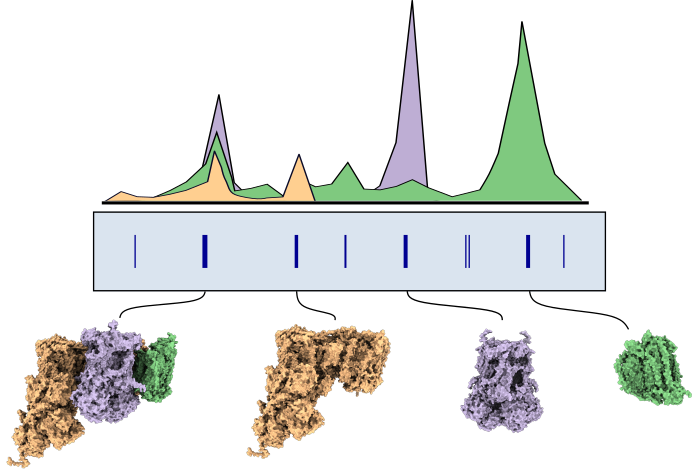
\includegraphics[width=0.5\textwidth]{Chapter.2/Figures/chapter_cover.png}
\vspace{1cm}

{Johannes F. Hevler\textsuperscript{*}, Marie V. Lukassen\textsuperscript{*}, Alfredo Cabrera-Orefic, Susanne Arnold, Matti F. Pronker, Vojtech Franc and Albert J.R. Heck}
\end{center} 

\begin{flushleft}
\vspace*{\fill}    
\rule{\textwidth}{1pt}\\[0cm]
\textbf{This chapter is based on work in the following publication:}\\
\footnotesize
\textbf{\emph{The EMBO Journal}} (2021), 40:e106174, doi:10.15252/embj.2020106174\\

\footnotesize
\vspace{0.3cm}
\begin{tabular}[t]{p{0.01\textwidth}p{0.90\textwidth}}
\textsuperscript{*} & These authors contributed equally to this work\\
\end{tabular}
\end{flushleft}

\newpage
\begin{abstract101} 
Cross-linking mass spectrometry has developed into an important method to study protein structures and interactions. The in-solution cross-linking workflows involve time and sample consuming steps and do not provide sensible solutions for differentiating cross-links obtained from co-occurring protein oligomers, complexes, or conformers. Here we developed a cross-linking workflow combining blue native PAGE with in-gel cross-linking mass spectrometry (IGX-MS). This workflow circumvents steps, such as buffer exchange and cross-linker concentration optimization. Additionally, IGX-MS enables the parallel analysis of co-occurring protein complexes using only small amounts of sample. Another benefit of IGX-MS, demonstrated by experiments on GroEL and purified bovine heart mitochondria, is the substantial reduction of undesired over-length cross-links compared to in-solution cross-linking. We next used IGX-MS to investigate the complement components C5, C6, and their hetero-dimeric C5b6 complex. The obtained cross-links were used to generate a refined structural model of the complement component C6, resembling C6 in its inactivated state. This finding shows that IGX-MS can provide new insights into the initial stages of the terminal complement pathway.
\end{abstract101}

\newpage

\section{Introduction}
Over the last decades, bimolecular mass spectrometry (MS), with its ability to analyze low amounts of samples with high speed and sensitivity, has evolved into a central pillar beneficial for integrative structural biology \cite{de_Souza_2020, Kaur_2019, Lossl_2016, Robinson_2019}. The structural MS toolbox contains multiple complementary approaches. Next to native MS and top-down MS, a variety of peptide-centric MS methods, such as thermal proteome profiling (TPP), limited proteolysis (LiP), hydrogen/deuterium exchange (HDX) MS and chemical cross-linking MS (XL-MS or CLMS), have emerged and enabled structural studies of a wide range of biomolecules \cite{Feng_2014, Heck_2008, Leitner_2010, Savitski_2014, Zheng_2019}. With recent advances in instrumentation, sample preparation, and data analysis, especially XL-MS has started to fulfill its potential to complement well established structural methods such as X-ray crystallography, nuclear magnetic resonance spectroscopy (NMR), and cryo-electron microscopy (cryo-EM) \cite{Leitner_2016, Matthew_Allen_Bullock_2016, Rappsilber_2011}. XL-MS has a particular utility to capture protein-protein interactions in solution by measuring spatial distance restraints, mirroring structural conformations of intact proteins. Concomitantly, a wide range of chemical cross-linkers have been explored so far, often relying on similar chemical principles \cite{Sinz_2003, Steigenberger_2020}. Most used cross-linkers are small, homo-bifunctional reagents, with two reactive moieties capable of covalently binding two nearby amino acids. The reactive groups are separated by a spacer arm of varying lengths, which can be gas-phase cleavable or non-cleavable, thereby determining different MS data acquisition methods \cite{Kao_2011, Leitner_2010, Muller_2010, Staros_1982}. Recent advances in search engines for more efficient identification of cross-linked peptides allowed structural studies of purified proteins or protein complexes, as well as large scale experiments with more complex samples like purified organelles or cell lysates, using buffer systems which aim to meet physiological relevant conditions \cite{Beveridge_2020, Chen_2019a, Gotze_2019, Klykov_2018}. A typical XL-MS workflow begins with the optimization of the cross-linker concentration. Next, a protein mixture is incubated with the cross-linking reagent, and the reaction is subsequently quenched to prevent the generation of unwanted random protein contacts. After (tryptic) digestion, cross-linked peptides are subjected to various pre-fractionation steps or enrichment strategies to distinguish them from the vast majority of unmodified peptides. Cross-linked residues are eventually identified using dedicated XL-MS search algorithms, providing structural information in the form of distance restraints, which can be utilized to guide computational homology modeling, refinement of flexible regions within structural models, protein-protein docking and the generation of protein interaction networks \cite{Albanese_2020, Bullock_2018, Iacobucci_2019, Kim_2018, Ryl_2020}. Currently, technological developments in XL-MS aim to further improve the cross-linking reaction efficiency and detection. The research is mainly focused on sample preparation techniques, MS fragmentation and enrichment strategies, data acquisition and analysis of cross-linked peptides, as well as the design of novel cross-linkers \cite{Chen_2019b, Dau_2019, Iacobucci_2018, Leitner_2012, Liu_2017, Mendes_2019, Steigenberger_2019}.\\
Although the latest advances significantly revised and reformed the field of XL-MS, some challenges remain. A central problem of XL-MS data analysis is the occurrence of both false-positive and false-negative cross-link identifications. Especially, the existence of proteins with highly dynamic/flexible conformations and the presence of co-occurring alike protein complexes (e.g., protein oligomers and co-occurring complexes sharing distinct sub-units) significantly complicate the analysis by current in-solution XL-MS approaches. Interaction specific cross-links are relevant as structural changes can be triggered by the presence of a binding partner or the environment, thereby eventually displaying a physiological relevant protein conformation \cite{de_Souza_2020, Feng_2014, Mannige_2014, Uversky_2011}. Additionally, when using too high cross-linker concentrations or too high protein concentrations, undesired artificial interactions are likely being picked up by XL-MS. In-solution XL-MS experiments, therefore, need careful experimental optimization of, in particular, the concentration of the proteins and the cross-linker. Unfortunately, these steps require considerable sample amounts (tens of micrograms) and extra experimental time.\\
Here we describe an alternative approach, performing in-gel cross-linking mass spectrometry (IGX-MS), re-discovering the great separation power of gel-electrophoresis. Prior to cross-linking, we load the samples and perform blue native polyacrylamide gel

\begin{figure*}[hbt!]
\center
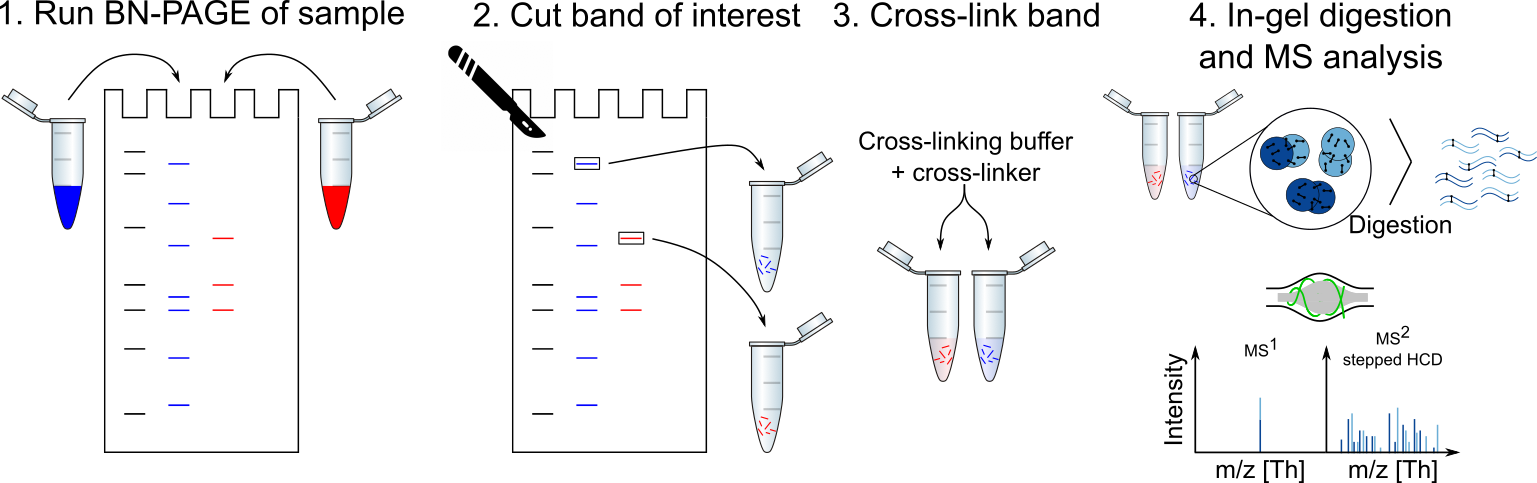
\includegraphics[]{Chapter.2/Figures/Figure1.png} 
\caption{\textbf{Combining BN-PAGE with IGX-MS.} In the first step, proteins and their assemblies are loaded and separated by BN-PAGE. The bands representing different protein assemblies are visualized after running the gel with Coomassie in the upper running buffer. The band(s) of interest are then excised from the gel and incubated with a cross-linking reagent in the cross-linking buffer. The cross-linking reaction is quenched and subsequently subjected to standard in-gel digestion. The extracted peptides are finally analyzed using cross-linking optimized parameters for the MS analysis.}
\label{fig:ch2_fig1}
\end{figure*}

electrophoresis (BN-PAGE), allowing the separation of distinct structural states of the proteins or protein complexes. The distinct bands are subsequently excised and cross-linked in the gel, enabling the measurement of conformation- and interaction-specific cross-links and derived distance restraints (\textbf{\autoref{fig:ch2_fig1}}). We show that this IGX-MS workflow has certain advantages compared to the in-solution based XL-MS methods. These include, amongst other things, no need for cross-linker concentration optimization, generation of conformation-specific cross-links, and relatively low sample amount requirements. Moreover, through IGX-MS data obtained for several protein assemblies, we provide evidence that proteins retain not only their quarternary but also their secondary and tertiary native structural states under BN-PAGE separation. To directly compare IGX-MS with in-solution XL-MS, we selected, as a proof-of-concept, the 14-mer \emph{Escherichia coli} GroEL chaperone and different respiratory chain complexes (super complex 1, complex I and complex V) from solubilized bovine heart mitochondria (BHM). Our experiments demonstrated that IGX-MS can accurately target specific subcomplexes co-existing in the protein complex mixtures and substantially reduce the number of (potentially false) over-length cross-links. Ultimately, we applied the optimized IGX-MS to investigate structures of the terminal complement proteins C5 and C6, which are involved in the initial steps towards the assembly of membrane attack complex (MAC). Our cross-linking data lead us to propose a refined alternative structural conformation of the complement component C6, providing new insights into the terminal complement pathway. In summary, our data show that BN-PAGE-based IGX-MS is a powerful tool, allowing the efficient generation of compositional- and interaction-specific distance constraints, with the potential of refining structural models of a large variety of protein assemblies, even when they co-occur in solution.

\section{Results}
\subsection*{BN-PAGE forms the basis for IGX-MS}
Blue native polyacrylamide gel electrophoresis, BN-PAGE, has proven to be a robust and sensitive method for separating protein complexes from various sample types. It requires only minimal sample amounts to sensitively estimate native protein molecular weights (Mw), respective compositional states, and protein-protein interactions. Further, proteins and protein complexes are thought to maintain not only their overall quarternary structural organization in the gel but also their secondary and tertiary structural organization, as they can still, after that, be subjected to further structural and functional analysis (2D crystallization, cryo-EM, in-gel activity assay) \cite{Poetsch_2000, Schafer_2006, Wittig_2007}.\\
Here, we combine BN-PAGE with XL-MS to efficiently isolate and investigate co-occurring protein oligomeric states and sub-complexes. We first determined whether proteins and protein complexes can be cross-linked in a BN gel. For this, 10 $\mu$g of purified E. Coli GroEL diluted in a Tris buffer was subjected to BN-PAGE as described previously \cite{Wittig_2006}. Bands corresponding to the native 14-mer GroEL (MW = 800 kDa) were excised from the BN-PAGE (\textbf{\autoref{fig:ch2_app_fig1}A}), and further, cut into small pieces and incubated with or without the cross-linker reagent DSS. Next, GroEL was extracted from the gel pieces and subsequently loaded onto a reducing SDS-PAGE (\textbf{\autoref{fig:ch2_app_fig1}B}). The control lane (no cross-linker) revealed only one distinct band at 57 kDa representing the GroEL monomers. In contrast, the BN-PAGE band that was incubated with DSS showed several additional high-molecular-weight bands above 100 kDa, indicating the successful cross-linking of GroEL subunits. Notably, the initial sample buffer (Tris) is incompatible with amine-reactive cross-linkers, as it contains primary amines that compete with the primary amines of Lysine residues, thereby significantly reducing the cross-link efficiency. Successful cross-linking of GroEL in-gel highlights the buffer exchange capacity of the BN-PAGE system, making additional buffer exchange steps (e.g., using molecular weight cut-off filters or dialysis), which would be required for in-solution cross-linking and eventually result in loss of sample, obsolete.

\subsection*{IGX-MS optimization is straightforward}
To prevent protein precipitation caused by over cross-linking, standard in-solution XL-MS crucially depends on using the optimal cross-linker concentration. For this, a subset of sample needs to be incubated with varying cross-linker concentrations prior to the experiment and subsequently analyzed by gel electrophoresis. The time and sample consuming optimization step led us to investigate the effect of varying cross-linker concentrations for IGX-MS experiments. GroEL was subjected to BN-PAGE, and relevant bands were cross-linked using the two different cross-linking reagent DSS and DSSO varying in five concentration steps from 0.5 to 5 mM. After quenching the cross-linking reaction with Tris, the protein-containing bands were prepared for MS analysis following a standard in-gel digestion procedure. Cross-links obtained for DSS and DSSO, and each concentration were validated by mapping them onto the GroEL structure (PDB ID: 1KP8), and lysine C$\alpha$-C$\alpha$ distances were obtained (textbf{Dataset EV1}). The distance distribution for both cross-linkers was highly similar at all used concentrations, and almost no cross-link distances over 30 Å were observed across the varying concentrations, indicating that IGX-MS is highly resistant against over cross-linking of proteins (\textbf{\autoref{fig:ch2_fig2}A}). Our data suggest that IGX-MS is also less hampered by\\

\begin{figure*}[hbt!]
\center
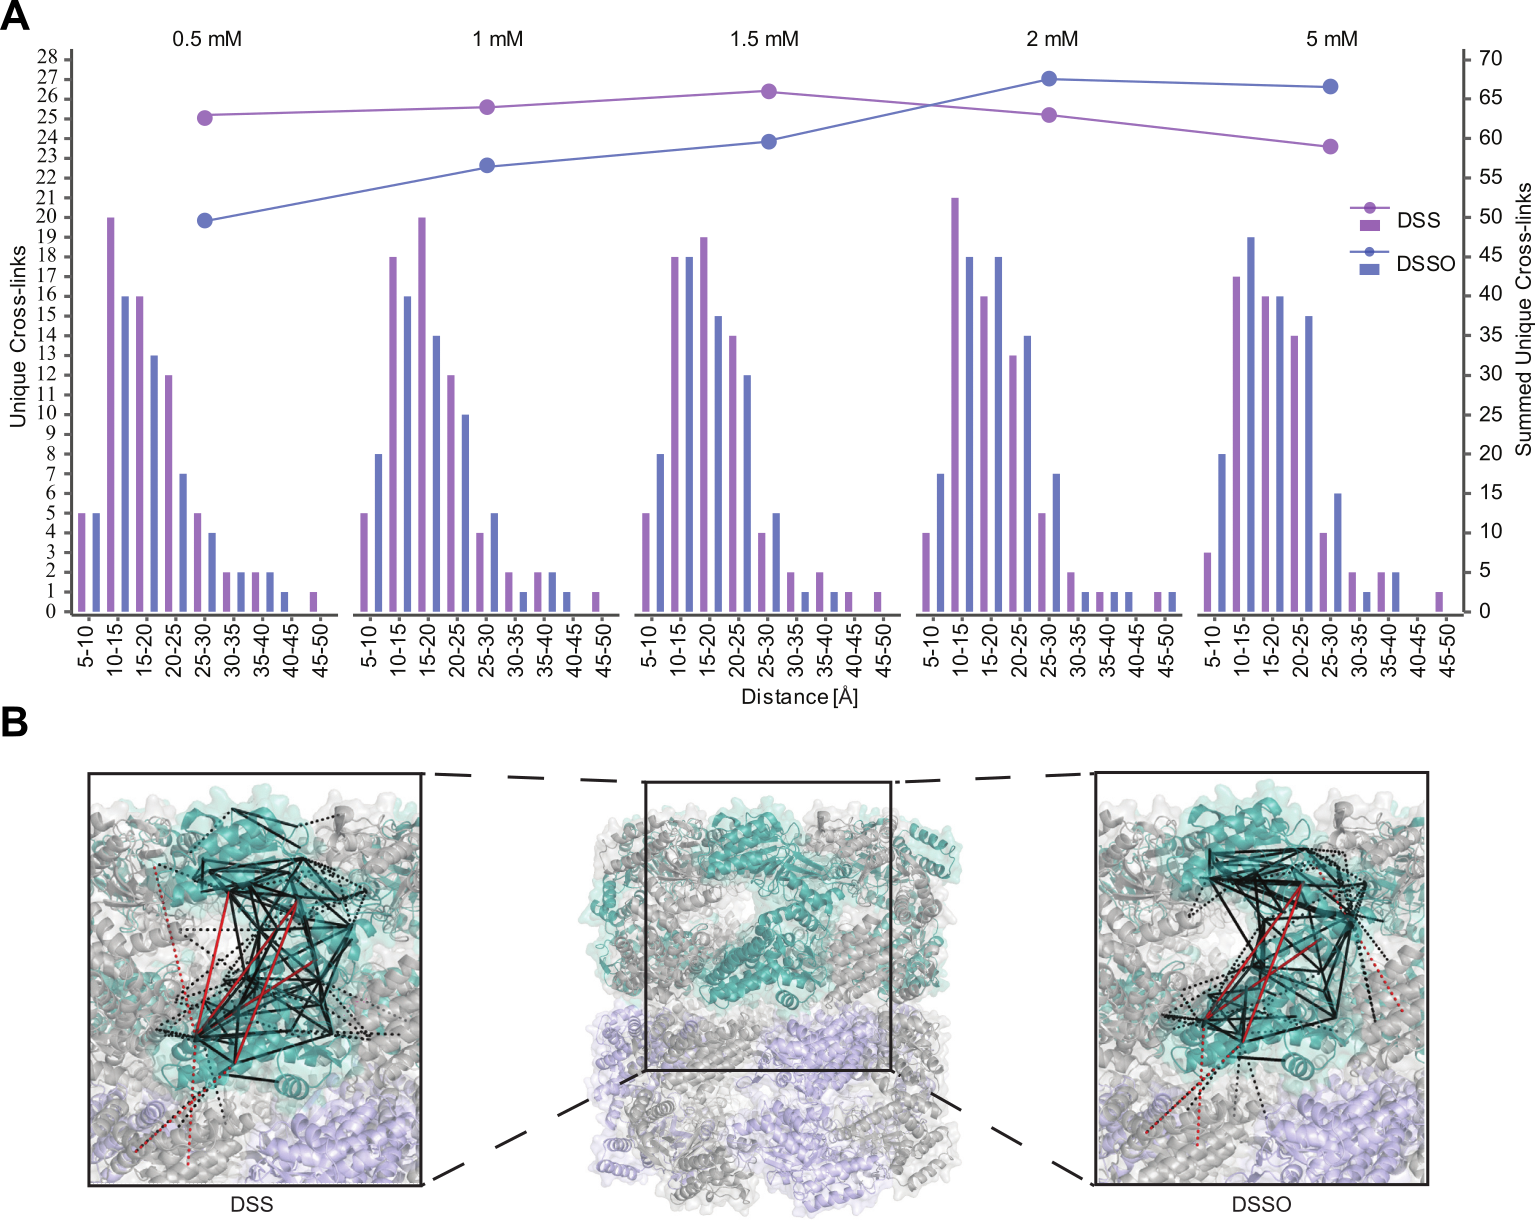
\includegraphics[]{Chapter.2/Figures/Figure2.png} 
\caption{\textbf{IGX-MS of GroEL using either DSS or DSSO at varying concentrations.} \textbf{A.} \emph{Escherichia coli} GroEL was cross-linked by IGX-MS using either DSS or DSSO at concentrations ranging from 0.5 to 5 mM. The identified cross-links were placed on the reported GroEL structure (PDB ID:1KP8), whereby the number of unique cross-linked lysine C$\alpha$-C$\alpha$ distances (using the left y-axis) were binned and as shown in bars. The summed number of unique cross-links obtained at each concentration is shown in lines using the right y-axis. \textbf{B.} Cross-links obtained by IGX-MS using DSS or DSSO plotted onto one subunit of GroEL (intra-links; solid lines) (PDB ID:1KP8) and neighboring subunits (inter-links; dashed lines). Cross-links agreeing with the set distance restraint of 30 Å are colored black, links exceeding the restraint are colored red.}
\label{fig:ch2_fig2}
\end{figure*}

unspecific cross-links. We also observed that the total number of unique cross-links was not affected by the concentration of DSS, and only marginally effected for DSSO as the obtained cross-links are slightly lower for concentrations below 2 mM (\textbf{\autoref{fig:ch2_fig2}A}). However, no significant difference was detected between 2 mM and 5 mM (\textbf{\autoref{fig:ch2_fig2}A}). The cross-linked sites onto the GroEL structure showed good consistency in cross-linked regions for both DSS and DSSO experiments (\textbf{\autoref{fig:ch2_fig2}B}, \textbf{Dataset EV1}). Finally, we compared the cross-linking results for each cross-linker and concentration across the three replicates, demonstrating excellent reproducibility of the IGX-MS experiments (\textbf{\autoref{fig:ch2_app_fig2}}). Based on these results, a DSS concentration of 1.5 mM and a DSSO concentration of 2 mM (\textbf{\autoref{fig:ch2_fig2}A}) were used for the subsequent experiments.

\subsection*{Direct comparison of IGX-MS and in-solution XL-MS}
BN-PAGE facilitates the distinction of oligomeric states, but it can also be particularly useful when protein complexes are reconstituted. In such experiments, one or more of the subunits may be (unwillingly) in excess. These preparations can then lead to false cross-link interpretations, as especially intra cross-links can originate from the free monomer subunit or subunit in the complex (which may exhibit another conformation). By comparing IGX-MS and in-solution XL-MS of GroEL, we aimed to access the relevance of this additional separation aspect and confirm that proteins maintain their native structural integrity during in-gel separation. First, for in-solution cross-linking, GroEL diluted in Tris buffer was buffer exchanged to PBS, and subsequently, the optimal cross-linker concentration was determined by SDS-PAGE to avoid over cross-linking (\textbf{\autoref{fig:ch2_app_fig3}A}). Next, the in-solution XL-MS sample was cross-linked with DSS, while the IGX-MS sample was cross-linked with both DSS and DSSO. Subsequent comparison of DSS- and DSSO-in-gel cross-linked samples showed a 53 \% overlap of identified cross-linked sites. Next, we directly compared in-solution XL-MS and IGX-MS. Although a significant number (60 \%) of DSS-in-gel cross-links was also detected by in-solution XL-MS (\textbf{\autoref{fig:ch2_fig3}A}), in-solution XL-MS resulted in a seemingly higher total number of unique cross-links compared to IGX-MS. First, we ruled out that the higher number of unique cross-links in-solution could be explained by insufficient extraction of long peptides from the gel, based on the observation that the detected cross-linked peptides displayed a similar length distribution (\textbf{\autoref{fig:ch2_app_fig3}B}). Plotting all the cross-links onto the GroEL structure revealed that a large portion of the "exclusive" in-solution cross-links originated from paired lysine residues separated by more than 30 Å, our distance cut-off. In contrast, virtually all IGX-MS cross-links remained below this cut-off (\textbf{\autoref{fig:ch2_fig3}B}, \textbf{Dataset EV1}). Therefore, we are convinced that the BN-PAGE gel separation removes the co-analysis of co-occurring protein assembly states and higher-order protein aggregates. The latter often leads to the observation of over-length cross-links in solution. Further, mapping and directly comparing the overlapped cross-links between the IGX-MS and in-solution XL-MS revealed high consistency of cross-linked sites, supporting that GroEL preserved its native conformation in the gel.

\begin{figure*}[hbt!]
\center
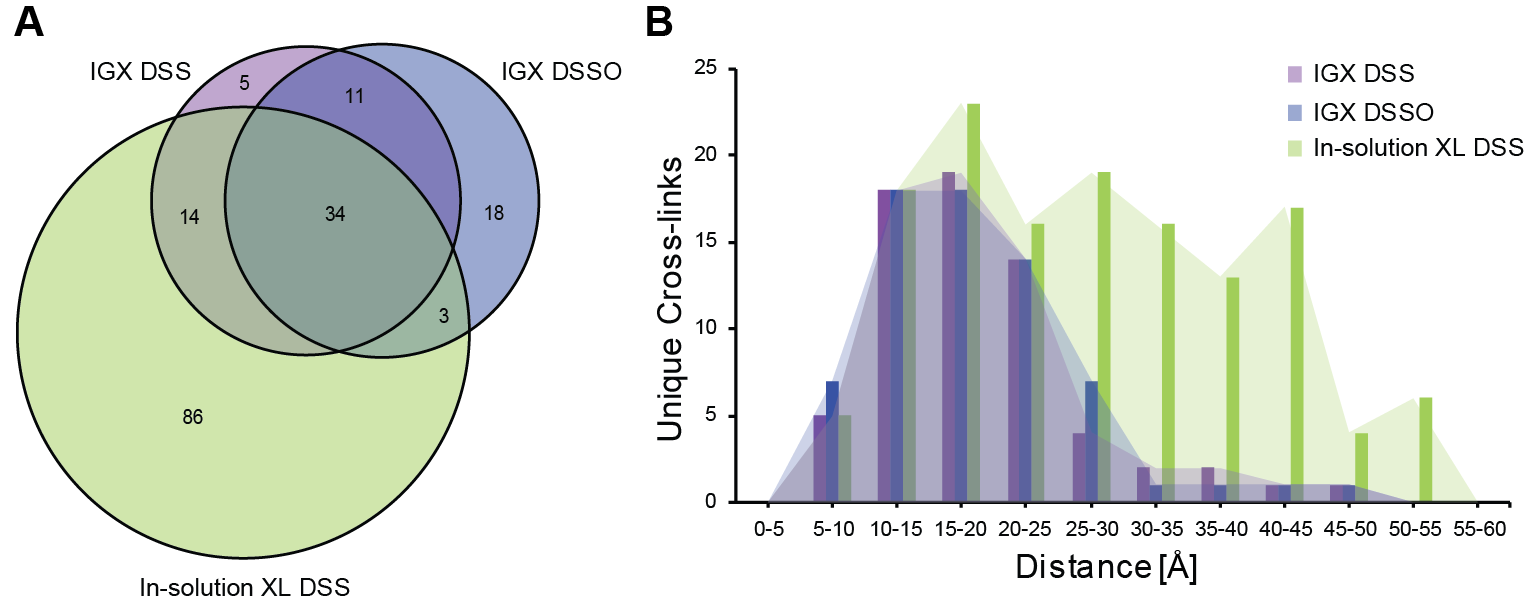
\includegraphics[]{Chapter.2/Figures/Figure3.png} 
\caption{\textbf{Comparison of IGX-MS and in-solution XL-MS of GroEL.} \textbf{A.} \emph{Escherichia coli} GroEL was subjected to in-solution XL-MS using 0.75 mM DSS. The resulting cross-links were compared to cross-links obtained by IGX-MS using DSS (1.5 mM) or DSSO (2 mM). The Venn diagram shows the overlap in the cross-links identified. \textbf{B.} Distribution of lysine C$\alpha$-C$\alpha$ distances of unique cross-links identified by IGX-MS (DSS or DSSO) or in-solution XL-MS plotted on the GroEL structure (PDB ID:1KP8).}
\label{fig:ch2_fig3}
\end{figure*}

\subsection*{IGX-MS facilitates the analysis of distinct co-occurring assemblies}
Proteins in cells or extracted from various biological sources can be part of multiple different complexes. Whether a protein is a free monomer or part of one or more protein complexes can substantially affect its structure. The identification of distinctive structural states of a protein by XL-MS in solution is often hampered, especially when the "free" monomer co-exist with the same protein being part of one or more complexes. For this reason, we investigated whether IGX-MS can exclusively obtain cross-links for proteins in a single configuration of the complex. As a first test-sample, we incubated GroEL with one of its known natural unfolded substrates, namely the bacteriophage T4 capsid protein (gp23, 56 kDa). Following incubation of GroEL with unfolded gp23, we analyzed this sample by BN-PAGE and observed three distinctive bands, corresponding to free GroEL and GroEL with one or two copies of gp23 bound (\textbf{\autoref{fig:ch2_app_fig4}A}). That GroEL can bind two substrate molecules (in the cis and trans ring) agrees with previously reported data \cite{van_Duijn_2006} and could be additionally confirmed by relative quantification of the subunits in the respective bands (\textbf{\autoref{fig:ch2_app_fig4}B}). In parallel cross-linking of each band, i.e., GroEL, GroEL:gp23 and GroEL:(gp23)2, with DSS, revealed interlinks between GroEL and gp23 exclusively in the middle and upper band whereby the primary inter-linked residues in GroEL were identified as K42, K122, and K272 (\textbf{Dataset EV2}). The site with most cross-links to gp23 was K272, located at the outer edge of the cavity (\textbf{\autoref{fig:ch2_app_fig4}C-D}). IGX-MS of each BN-PAGE bands enabled the identification of protein compositional specific distance restraints, which would have been impossible by in-solution XL-MS without additional experimental steps.\\
Next, we assessed the capabilities of IGX on a more complex sample and subjected 20 $\mu$g of purified bovine heart mitochondria (BHM), solubilized with digitonin, to BN-PAGE (\textbf{\autoref{fig:ch2_fig4}A}). It is well-known that BN-PAGE can separate and visualize the different complexes of the mitochondrial respiratory chain, including many of the co-occurring super-complexes \cite{Schagger_2000}. The band corresponding to the monomeric form of complex V (the well-studied ATP synthase, which can also be abundantly present in a V2 dimeric form), was excised and subjected to IGX-MS using DSS (\textbf{\autoref{fig:ch2_fig4}A}). The detected cross-links were plotted onto the 3D structure (PDB ID: 5ARA) and compared to cross-links detected in a previously published data set from our lab, by in-solution XL-MS \cite{Liu_2018} (\textbf{\autoref{fig:ch2_fig4}B}, \textbf{Dataset EV3}). Visualizing the detected IGX-MS- and in-solution XL-MS cross-linked regions revealed their high consistency, indicating that these membrane protein complexes largely retain their quarternary, tertiary, and secondary structures in the BN-PAGE gel. Similar to the previous in-solution XL-MS experiments, only solvent-accessible regions of complex V subunits (which in intact mitochondria are facing the matrix) were detected in the IGX data. Further, we found that ATP5IF, a known inhibitor of the ATPase, was associated with the monomeric ATP synthase (\textbf{\autoref{fig:ch2_fig4}C}). Detected cross-links from the inhibitor to ATP5F1E, ATP5F1D, ATP5F1C, and ATP5F1B agree with the previously reported binding interface of ATP5IF and the ATPase \cite{Gledhill_2007}. In-solution XL-MS resulted in a higher number of unique cross-links (248 vs. 53 for IGX). However, like for GroEL, the C$\alpha$-C$\alpha$ distance distribution revealed that many in-solution XL-MS cross-links are well above the 30 Å cut-off (149 unique cross-links). The IGX-MS cross-links are predominantly below this set cut-off (only two unique cross-links above), highlighting the accordance of the IGX-MS generated restrains with the previously published structure of monomeric ATPase (\textbf{\autoref{fig:ch2_fig4}D}, \textbf{Dataset EV3}). We argue that some of these over-length cross-links detected by in-solution XL-MS may originate from co-occurring dimeric complex V or other ATPase conformations induced upon binding of one (or several) of its many previously identified interactors \cite{Liu_2018, Ryl_2020, Schweppe_2017}. Additionally, IGX-MS generated cross-links exclusively describe the interaction of ATP5IF to monomeric ATP synthase. In contrast, in-solution XL-MS generated cross-links most-likely reflect distance restraints for different assembly states of ATP synthase (e.g., monomeric/dimeric ATP synthase with and without ATP5IF). To further showcase the ability of IGX-MS to generate assembly state-specific cross-links, bands corresponding to monomeric complex I (CI) and the super complex 1 (S1) were excised and subjected to IGX-MS using DSS (\textbf{\autoref{fig:ch2_app_fig5}A}). For both assembly states, a similar interaction network between the CI subunits was observed (\textbf{\autoref{fig:ch2_app_fig5}A}, \textbf{Dataset EV3}), revealing subunits that are in close proximity to each other in assembled CI (PDB ID: 5GUP). Cross-links detected for the super complex 1 (S1) revealed inter-complex links between\\

\begin{figure*}[hbt!]
\center
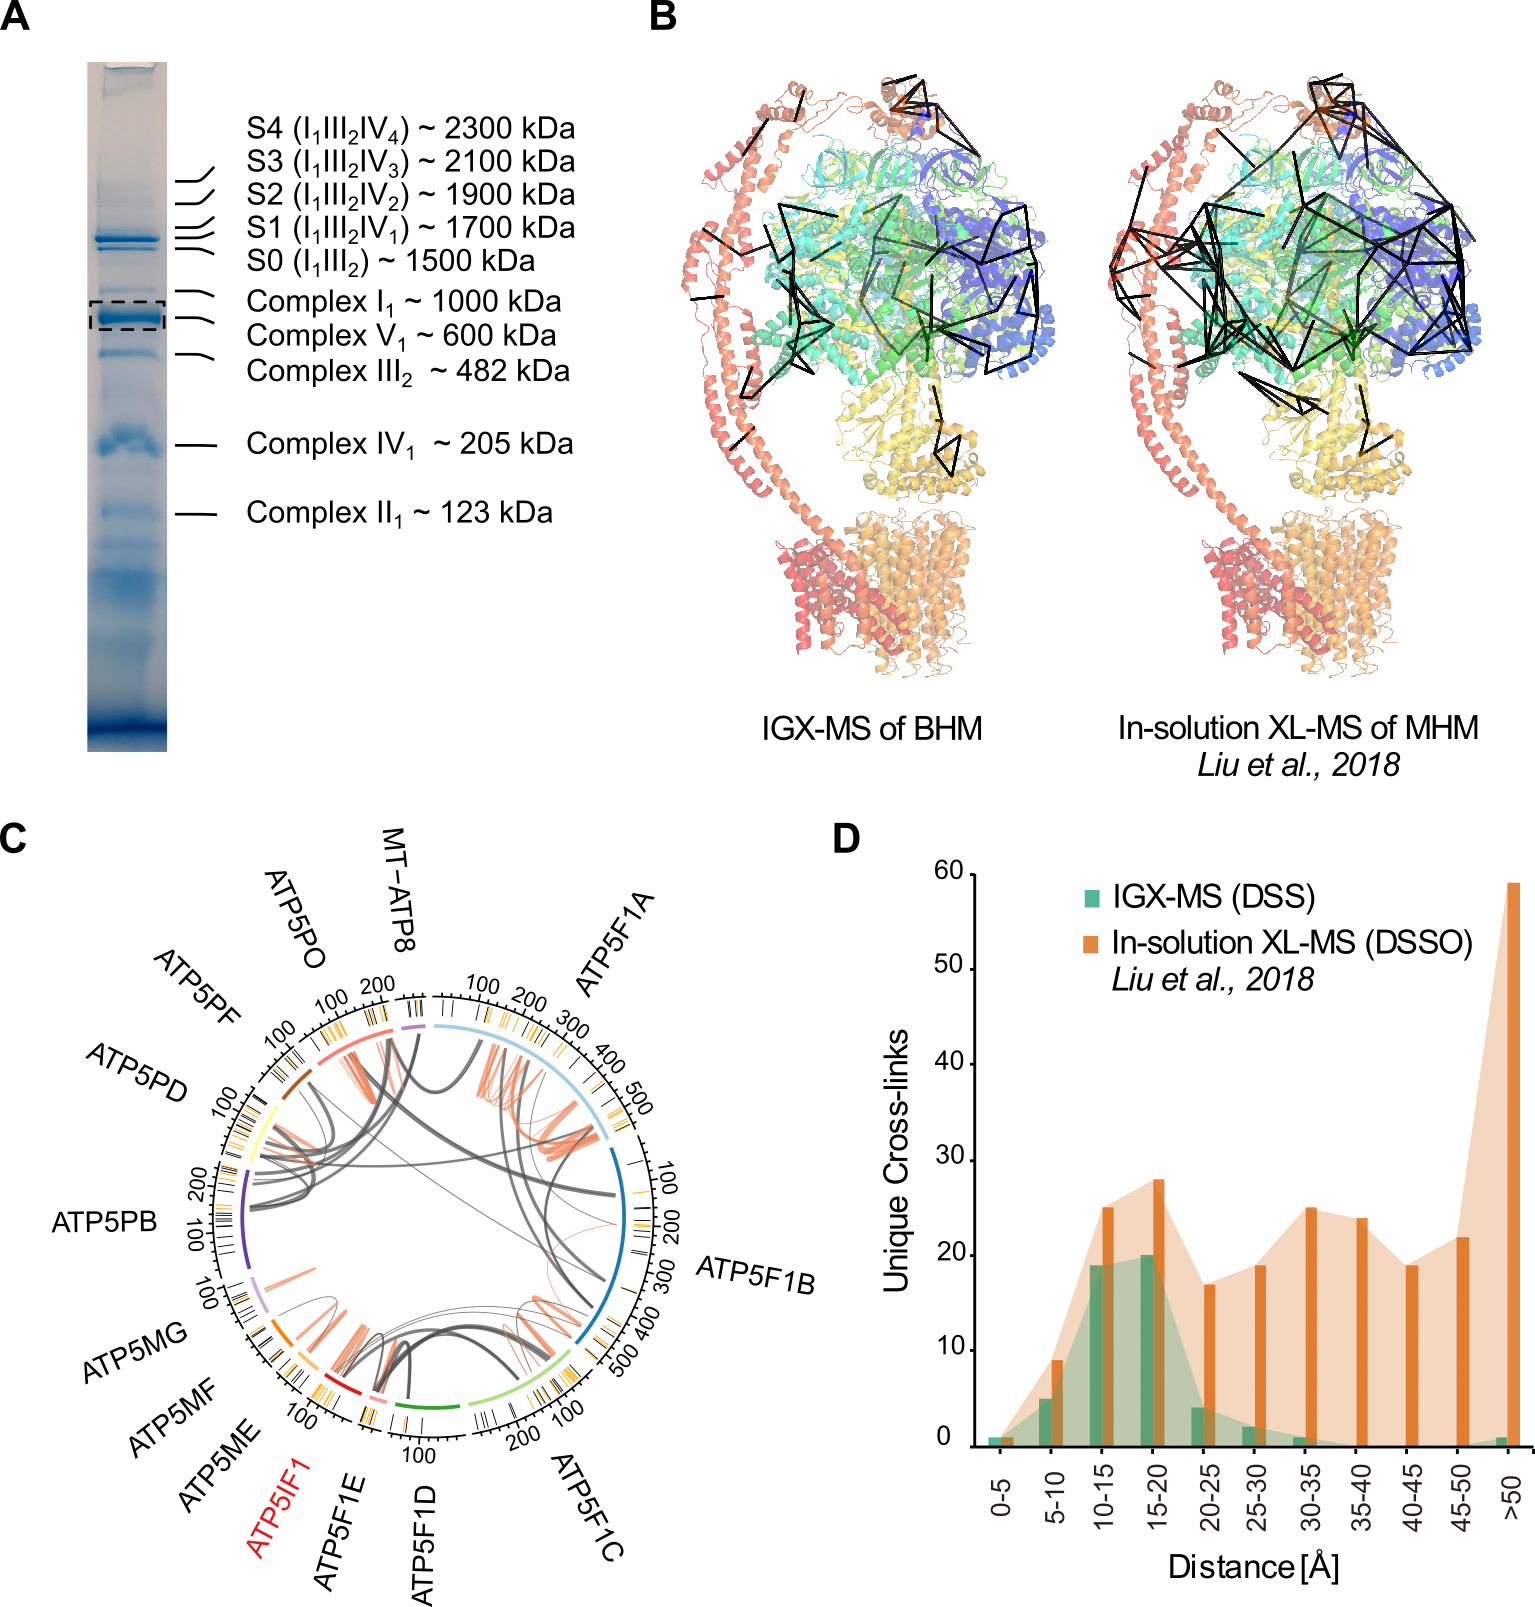
\includegraphics[]{Chapter.2/Figures/Figure4.png} 
\caption{\textbf{Selective cross-linking of the ATP synthase monomer from bovine heart mitochondria (BHM) by IGX-MS.} \textbf{A.} BN-PAGE of 20 $\mu$g solubilized BHM with several of the distinct complexes annotated. The dashed box indicates the monomeric ATP synthase (complex V) band subjected to IGX-MS. Annotation of protein bands was done following a previously published study \cite{Wittig_2010}. \textbf{B.} Unique cross-links < 30 Å identified by IGX-MS in this study (left) or by Liu \emph{et al} \cite{Liu_2018} using in-solution XL-MS plotted on the ATP synthase structure (PDB ID:5ARA). \textbf{C.} Circos plot of cross-linked ATP synthase subunits and the ATP synthase inhibitor (ATP5IF1) identified by IGX-MS. The position of the lysine residues is shown in the outer-ring, and cross-linked residues are colored dark orange. Orange lines represent intra-links while inter-links are colored dark gray. Thickness of the cross-link lines correlates to the number of detected cross-linked spectra matches (CSMs). \textbf{D.} Distribution of lysine C$\alpha$-C$\alpha$ distances of unique cross-links identified by IGX-MS or in-solution XL-MS \cite{Liu_2018} using DSS (1.5 mM) or DSSO (0.5 mM), respectively.}
\label{fig:ch2_fig4}
\end{figure*}
\clearpage

NDUFB4 (a subunit of complex I), UQCRC1, UQCRB (both subunits of complex III), COX7A1, and COX5B (both subunits of complex IV). This data agrees with the previously published structure \cite{Wu_2016}, which identified respective subunits in the interface regions of S1 (\textbf{\autoref{fig:ch2_app_fig5}A}, PDB ID: 5GUP). As reported for the ATP synthase, IGX-MS data for CI (monomeric and S1) closely resembles the previously reported in-solution XL-MS data \cite{Liu_2018} (\textbf{Dataset EV3}). Moreover, the targeted approach of IGX-MS allowed us to distinguish cross-links coming from monomeric CI or CI as part of S1, whereas in-solution XL-MS data represents a mixture of all the different assembly states (e.g., monomeric and S0-S4) (\textbf{\autoref{fig:ch2_fig4}A}, \textbf{\autoref{fig:ch2_app_fig5}B}).
In summary, comparing the IGX-MS and in-solution XL-MS cross-links for mitochondrial complex V, complex I and S1 highlights the capability of IGX-MS to generate sufficient, reliable and assembly-specific distance restraints.

\subsection*{Structural features of the complement proteins C5 and C6 and how these adapt when complexed into C5b6}
The terminal pathway of the complement system is mediated by sequentially interacting proteins (a.o. C5 to C9) that undergo various conformational changes in response to interactions with each other and the membrane environment \cite{Bajic_2015, Bayly-Jones_2017, Hadders_2012, Schatz-Jakobsen_2016}. In this process, membrane attack complex (MAC) is typically formed on the membrane of bacteria or pathogens, which leads to their elimination. Briefly, C6 binds to C5b, which originates from C5 by proteolytic cleavage. The resulting C5b6 complex binds C7, C8, and C9 sequentially, forming the C5b-9 complex. This complex is assembled onto the bacterial membrane and combines with polymerizing C9 molecules to create a lytic pore termed MAC \cite{Esser_1994}. Several structures of the different components of the terminal pathway have been explored by X-ray crystallography and electron microscopy (EM) \cite{Aleshin_2012, DiScipio_1988, DiScipio_1989, Fredslund_2008, Hadders_2012, Lovelace_2011, Menny_2018}. Especially well-resolved structures of monomeric C5, C6, and C5b6 contributed to understanding conformational changes that these proteins undergo in forming the C5b6 complex \cite{Aleshin_2012, Fredslund_2008, Hadders_2012}. We set out to investigate these different conformations by applying IGX-MS on monomeric C5, monomeric C6, and the hetero-dimeric C5b6 complex. Therefore, the BN-PAGE bands representing monomeric C5, monomeric C6, and C5b6 were subjected to IGX-MS (\textbf{\autoref{fig:ch2_app_fig6}A}). Cross-links obtained for both C5 and complexed C5b were in good agreement with the respective available structural models (PDB ID: 3CU7 and 4A5W) (\textbf{\autoref{fig:ch2_fig5}A,B}, \textbf{Dataset EV4}). In the C-terminal region of free C5, we detected some cross-links that exceed the distance restraint. This region is known to undergo significant structural rearrangements, as it adopts a more open conformation after conversion to C5b (\textbf{\autoref{fig:ch2_fig5}A}, \textbf{\autoref{fig:ch2_app_fig6}B}).

\begin{figure*}[b!]
\center
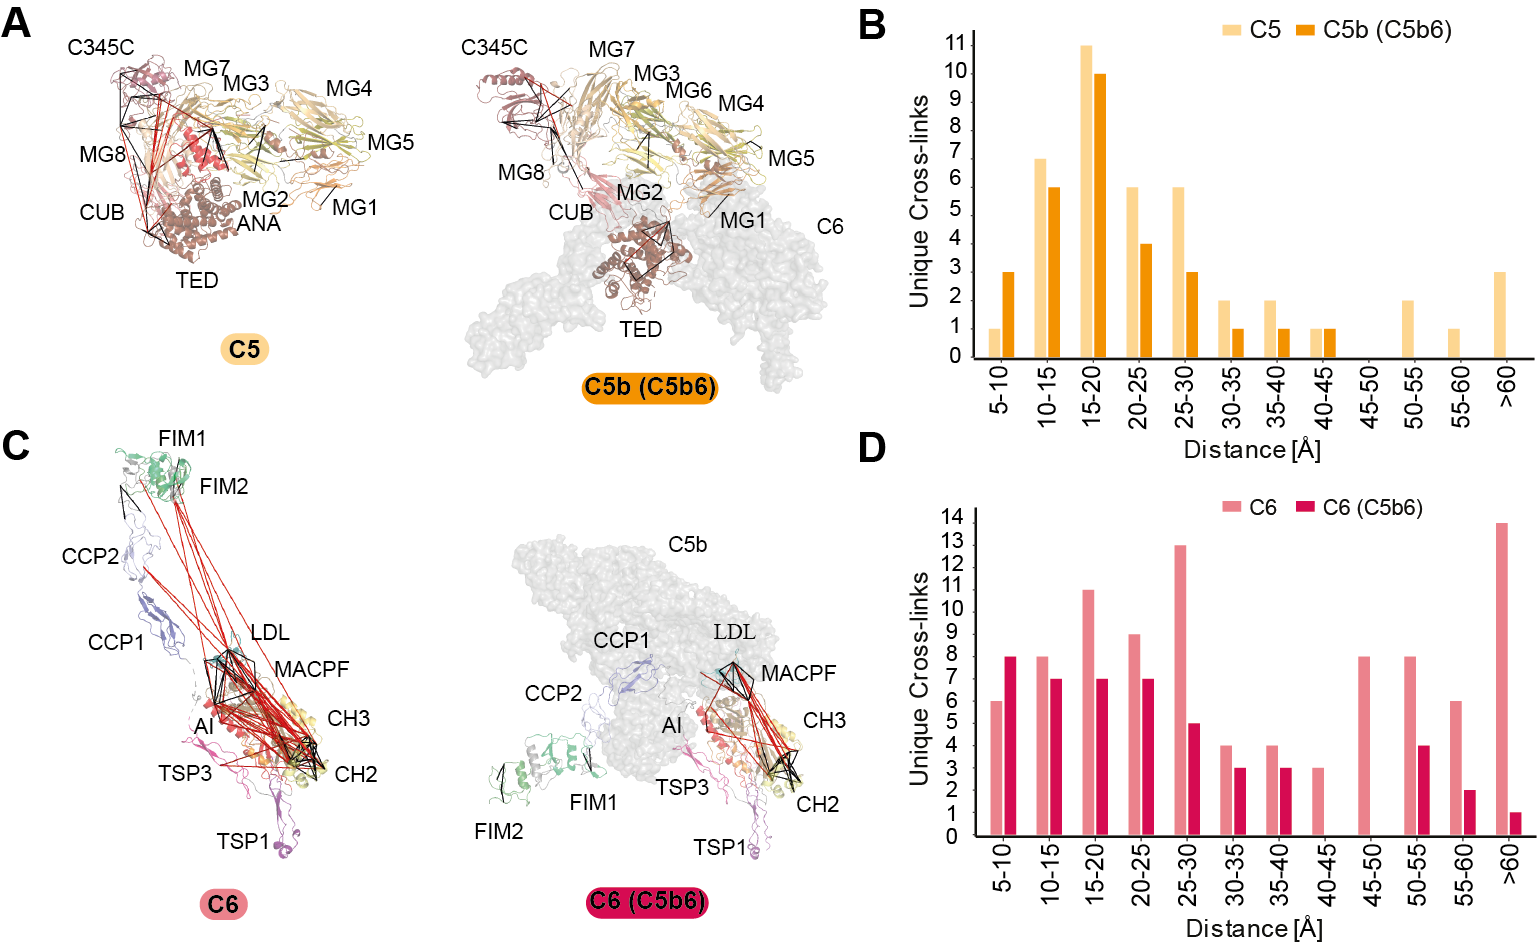
\includegraphics[]{Chapter.2/Figures/Figure5.png} 
\caption{\textbf{IGX-MS of the monomeric complement proteins C5 and C6, and the hetero-dimeric C5b6 complex.} \textbf{A.} Cross-links of monomeric C5 (left) and from C5b incorporated in the C5b6 complex (right) plotted on the respective available structural models (PDB ID: 3CU7 and 4A5W, respectively). The red lines indicate distances >30 Å. The different domains of C5 are indicated, and C6 within the C5b6 complex is shown in grey. \textbf{B.} Distribution of lysine C$\alpha$-C$\alpha$ distances of unique cross-links identified by IGX-MS in monomeric C5 (light orange) and C5b when part of the C5b6 complex (dark orange). \textbf{C.} Cross-links of monomeric C6 (left) and C6 incorporated in the C5b6 complex (right) plotted on the respective structural models (PDB ID: 3T5O and 4A5W, respectively). The red lines indicate distances >30 Å. The different domains of C6 are indicated, and C5b within the C5b6 complex is shown in grey. \textbf{D.} Distribution of lysine C$\alpha$-C$\alpha$ distances of unique cross-links identified by IGX-MS in monomeric C6 (light red) or C6 when incoprorated within the C5b6 complex.}
\label{fig:ch2_fig5}
\end{figure*}
\clearpage

Likewise, cross-links obtained for monomeric C6 and complexed C6 were plotted onto previously reported structural models (PDB ID: 3T5O and 4A5W) (\textbf{\autoref{fig:ch2_fig5}C}, \textbf{Dataset EV4}). Cross-links obtained for C6 when present in C5b6 were consistent with the previously published C5b6 structure (PDB ID: 4A5W). In contrast, cross-links obtained for monomeric C6 (PDB ID: 3T5O) did not substantiate the existing structural model and showed a noticeable bimodal distance distribution (\textbf{\autoref{fig:ch2_fig5}D}). Full-length C6 is composed of three thrombospondin (TSP) domains, a membrane attack complex/perforin (MACPF) domain, an LDL-receptor class A (LDL) domain, and an epidermal growth factor-like (EGF) domain. The EGF domain is followed by the C5b-binding domain composed of two complement control protein domains (CCP1 and CCP2) and two C-terminal factor I modules (FIM1 and FIM2), which are connected to the main body through a partially unresolved flexible linker (\textbf{\autoref{fig:ch2_fig5}C}). Interestingly, a high number of over-length cross-links (> 30 Å) in monomeric C6 were observed between the LDL domain and the MACPF, as well as within the MACPF domain itself. Cross-links exceeding the distance constraint within the MACPF are connecting the previously described autoinhibitory region (AI, residue 480-522) to two $\sim$50-residue helical clusters (CH1, residue 236-288; CH2 residue 363-416) (\textbf{\autoref{fig:ch2_fig5}C}, \textbf{\autoref{fig:ch2_app_fig6}C}) \cite{Hadders_2012}. Secondly, several over-length cross-links were observed between the FIM2 domain and the LDL and MACPF domain residues. These over-length cross-links are nearly exclusively detected for monomeric C6 and not for C6 when present in C5b6 (\textbf{\autoref{fig:ch2_fig5}C}, \textbf{\autoref{fig:ch2_app_fig6}C}).

\subsection*{Cross-link guided structural refinement of monomeric free C6}
Monomeric C6 displayed an intolerably high number of over-length cross-links suggesting that an alternative conformation of monomeric free C6 may (co-)exist. Based on identifying the lysine residues involved in these over-length cross-links, such an alternative structure would include re-positioning of the MACPF-, LDL- and the C5b-binding domains. We sought to define a structural model for monomeric C6 in two consecutive modeling steps. Our final refined model (\textbf{\autoref{fig:ch2_fig6}A}) retained the characteristic sequence-specific secondary structure elements and is only missing the flexible linker domain (residues 591-619), for which no confident distance restraints were available, likely due to the lack of lysine residues in this region. The missing linker comprises 28 amino acids, resulting in an 81 Å-gap in the IGX-MS driven model of C6 (\textbf{\autoref{fig:ch2_fig6}A} - black dots). Considering an average residue length of 3.4 - 4 Å, the length of this linker translates to 95.2 - 112 Å, which is sufficient to accommodate the produced gap \cite{Ainavarapu_2007}. When comparing the inter-domain rotation angles and domain centroid displacements between our model and the monomeric C6 X-ray structure (PDB ID: 3T5O), it becomes apparent that the main body (TSP1-1-TSP1-2-LDL-MACPF-EGF-TSP1-3) and the C5b-binding region (CCP1-CCP2-FIM1-FIM2) undergo a significant motion to each other (angle of 32 ° and displacement of 110.0 Å between TSP1-3 and FIM1 - \textbf{\autoref{fig:ch2_fig6}B}, \textbf{Table EV1}). On the other hand, the C5b-binding region moves almost like a single body with small inter-domain angles and displacements (largest angle of 2 ° and largest displacement of 1.1 Å). Within the main body, substantial domain reorientations can also be observed; in particular between EGF and TSP1-3 (angle of 83 ° and displacement of 16.7 Å), between TSP1-1 and TSP1-2 (angle of 42 ° and displacement of 19.7 Å), and between EGF and TSP1-3 (angle of 29 ° and displacement of 16.3 Å) (\textbf{\autoref{fig:ch2_fig6}B}, \textbf{Table EV1}). Further, when comparing the MACPF domain of the IGX-MS driven model to the previously reported structures of monomeric, complexed, and activated C6, noticeable intra-domain differences are obtained (\textbf{\autoref{fig:ch2_app_fig7}A-D}). Overall, the MACPF domain comprises a central four-stranded $\beta$-sheet, an AI region dominated by a linchpin helix, and three helical clusters (CH1-3) of which CH1 and CH2 unfold upon C6 activation (\textbf{\autoref{fig:ch2_app_fig7}A}). Closer examining the MACPF domain of the monomeric C6 X-ray structure (\textbf{\autoref{fig:ch2_app_fig7}B}) revealed a remarkable conformational resemblance with the MACPF domains of complexed C6 (\textbf{\autoref{fig:ch2_app_fig7}C}) and activated C6 (\textbf{\autoref{fig:ch2_app_fig7}D}). Interestingly, in our cross-linked driven structural model, we obtained a different conformational orientation of the regions within the MACPF domain (\textbf{\autoref{fig:ch2_app_fig7}A}). A clear re-positioning of the linchpin helix (part of the AI region), as well as the CH1 and CH2 cluster, can be delineated when compared to the MACPF of the X-ray structure (\textbf{\autoref{fig:ch2_app_fig7}E}). Here, the linchpin helix of the IGX-MS driven model (sand-colored structure) is tilted towards the central $\beta$-sheets and the helical clusters (CH1-3) (\textbf{\autoref{fig:ch2_app_fig7}F}). Additionally, the CH1 and CH2 domains are shown to be re-located, with the CH1 domain moved upwards, and the CH2 domain tilted towards the linchpin helix when compared to the MACPF domains of the previously reported monomeric, complexed and activated C6 structures (\textbf{\autoref{fig:ch2_app_fig7}F}). Conclusively, the structural rearrangements, guided by our IGX-MS data, result in a more closed conformation of the MACPF domain for free monomeric C6. Besides over-length cross-links within the MACPF domain, we detected eight cross-link restraints between the C5b-binding domain (specifically CCP2, FIM1, and FIM2) and LDL- and the MACPF-domain (specifically CH2) (\textbf{\autoref{fig:ch2_app_fig8}A}). The domains that are usually involved in the binding interface of C6 and C5b (CCP1 and CCP2 - see \textbf{\autoref{fig:ch2_fig5}C}) are in our model predicted to wrap around the MACPF domain, sharing an interaction interface with its CH2 and CH3 cluster (\textbf{\autoref{fig:ch2_fig6}A}, \textbf{\autoref{fig:ch2_app_fig8}B}). The FIM2 domain formes an interaction interface with residues of the TSP2, LDL, and MACPF domain, thereby locking the C5b-binding domain to the main body of C6 (\textbf{\autoref{fig:ch2_fig6}A-B}, \textbf{\autoref{fig:ch2_app_fig8}C}, \textbf{Dataset EV5}). This observation is in sharp contrast to the reported X-ray structure, in which the C5b-binding domain shows an "elongated" conformation, with no interaction interface between the mentioned domains (\textbf{\autoref{fig:ch2_fig6}B}). Further, we generated contact-maps to assess the overlap of cross-link data with the C6 X-ray structure and the IGX-MS driven model. The IGX-MS driven model provides new contact possibilities between the C5b-binding domain and the LDL-, and MACPF domain as well as within the MACPF domain (\textbf{\autoref{fig:ch2_fig6}C}), thereby significantly improving the overlap between the IGX and reported structural data (\textbf{\autoref{fig:ch2_fig6}D}, \textbf{Dataset EV4} and \textbf{Dataset EV6}). To validate the structural model for C6, we additionally performed an in-solution XL-MS experiment on purified C6. Firstly, the optimal cross-linker concentration was determined by incubating C6 with varying DSS concentrations (0-1.5 mM) (\textbf{\autoref{fig:ch2_app_fig9}A}). The optimization also revealed the formation of low amounts of dimeric C6 at all used crosslinking concentrations (\textbf{\autoref{fig:ch2_app_fig9}A}). Thus, an additional SDS-PAGE was performed following the in-solution cross-linking reaction (using 0.25 mM DSS)

\begin{figure*}[b!]
\center
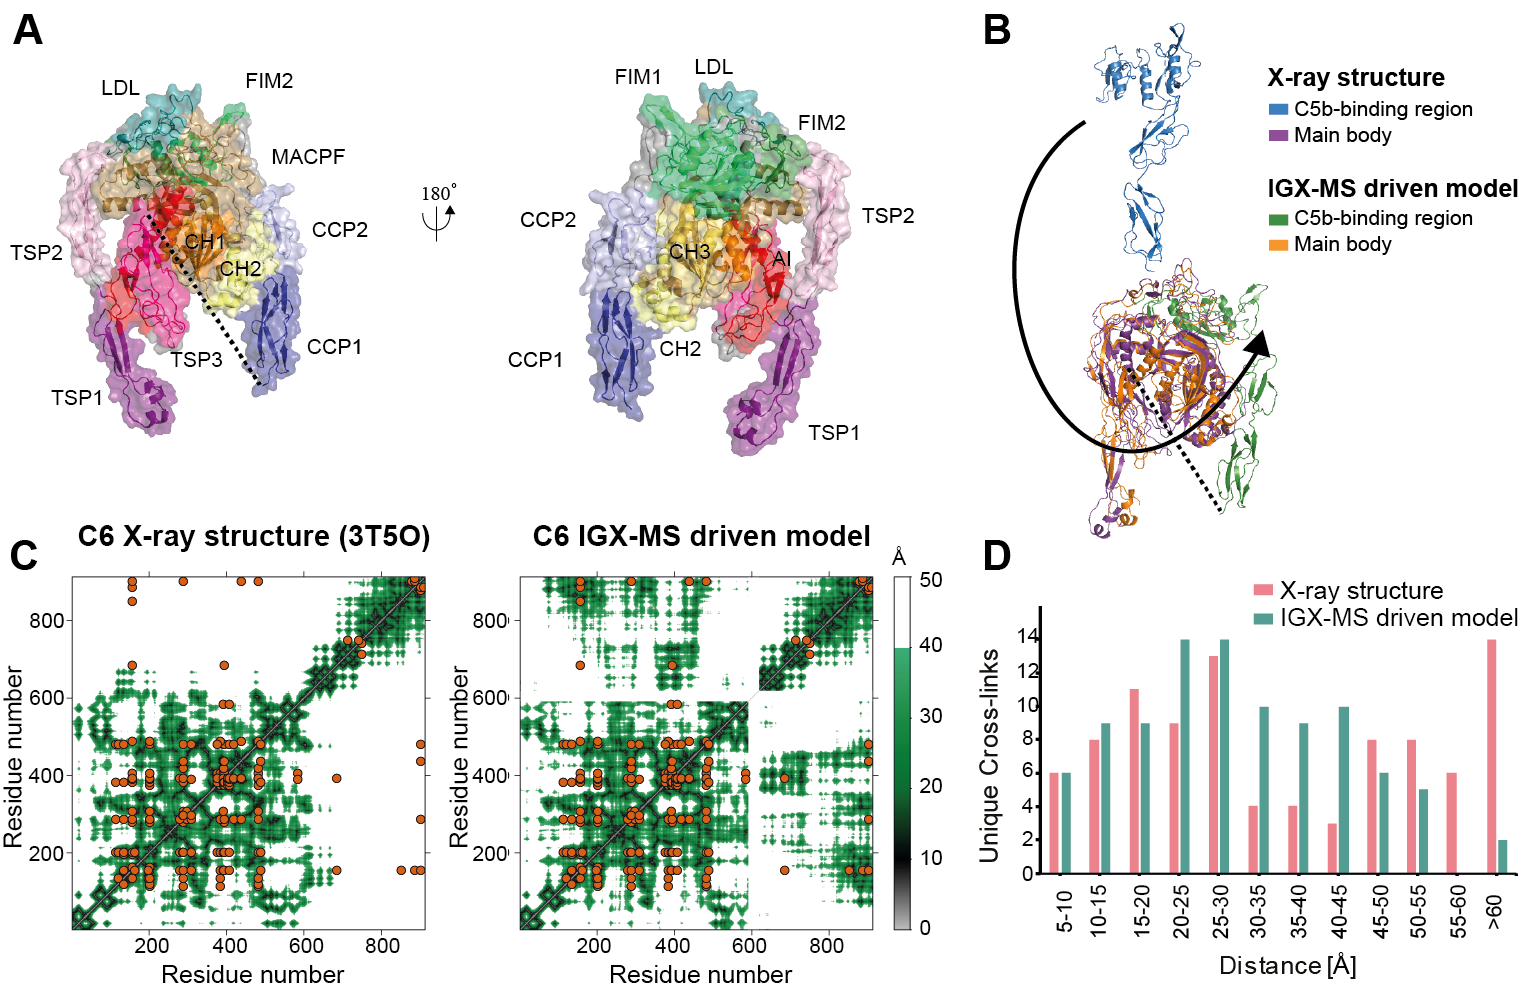
\includegraphics[]{Chapter.2/Figures/Figure6.png} 
\caption{\textbf{IGX-MS driven refined structural model of monomeric C6.} \textbf{A.} IGX-MS driven homology model of monomeric free C6 depicted in two different orientations. Black dots indicate the few missing amino acids (residue 591-619, spanning about 81 Å) covering the linker region between the main body and C5b-binding region. \textbf{B.} Superpositioning of C6 IGX-MS driven model (purple and green surface) and C6 X-ray structure (orange and blue surface; PDB ID: 3T5O). Black dots indicate the few missing amino acids (residue 591-619) covering the linker region between the main body and C5b-binding region. \textbf{C.} Contact maps with cross-linked residues (orange dots) of C6 X-ray structure (PDB ID: 3T5O, left panel) and IGX-MS driven C6 model (right panel). The colored density represents a contact relationship smaller than 40 Å of individual residues. White density represents a contact relationship bigger than 40 Å of individual residues. \textbf{D.} Distribution of lysine C$\alpha$-C$\alpha$ distances of unique cross-links identified by IGX-MS for monomeric C6 when plotted on the reported X-ray structure (pink bars, PDB ID: 3T5O) and the IGX-MS driven refined structural model (green bars).}
\label{fig:ch2_fig6}
\end{figure*}

to selectively detect crosslinks for monomeric C6. The in-solution generated cross-links were in agreement with the IGX-MS generated cross-links for monomeric C6, thereby suggesting a re-positioning of the MACPF-, LDL- and the C5b-binding domains (\textbf{\autoref{fig:ch2_app_fig9}B}). Finally, like for IGX-MS generated cross-links, the by in-solution XL-MS generated distance restraints for monomeric C6 are better satisfied for our cross-linked refined structural model than the X-ray structure (mean cross-link distance 26.2 Å vs. 41.7 Å - \textbf{\autoref{fig:ch2_app_fig9}C}).

\section{Discussion}
In-solution XL-MS has become a useful tool to study protein structures and protein-protein interactions \cite{Henry_2018, Koukos_2020, Liu_2014}. Even though the technology of in-solution XL-MS advanced substantially over the last decade, there are still quite a few challenges left. The current in-solution XL-MS method is time and labor demanding. Further, in-solution XL-MS requires a considerable amount of sample, which is necessary for optimizing the cross-linker concentration and the enrichment of cross-linked peptides. Also, in-solution co-occurring protein oligomers and distinct protein complexes within a sample can complicate the structural analysis. Unfortunately, current in-solution XL-MS workflows need further experimental steps to separate these protein complexes and potentially demand higher starting material amounts.\\
Here we introduce IGX-MS, an alternative approach that aims to tackle some of the challenges of in-solution XL-MS mentioned above. Firstly, we demonstrate the feasibility of cross-linking proteins in a BN-PAGE gel environment. We show that the efficiency of the in-gel cross-linking reaction is cross-linker- and also concentration-independent (DSS and DSSO work equally well). The latter makes the time- and sample consuming cross-linker concentration optimization obsolete. BN-PAGE combined with IGX-MS is very sensitive, requiring only a few micrograms of a protein sample to dissect and study different co-occurring protein complexes. These features reduce sample preparation time as no purification of a protein/ protein complex of interest is needed and enables the analysis of samples that are only available in minimal quantities (and therefore not susceptible to conventionally used purification methods for in-solution XL-MS). Another step, which can be omitted by using IGX-MS, is the samples's buffer exchange into a cross-link compatible buffer since it occurs already in the gel. The IGX-MS data presented here is hallmarked by high reproducibility, and to a large extent, the observed cross-links agree with those found by parallel in-solution cross-links. We find this as an important conclusion. It supports that proteins in the BN-PAGE gel maintain their native quarternary, tertiary, and secondary structures, as previously suggested \cite{Poetsch_2000, Schafer_2006, Wittig_2007}. Compared to in-solution XL-MS, IGX-MS shows a desired significant reduction of over-length cross-links when plotted on reported structures. A closer investigation of in-solution and in-gel cross-links revealed that IGX-MS generates protein state-specific cross-links with fewer undesired cross-linking products than in-solution XL-MS. This specificity is mainly achieved due to the option to precisely cross-link a specific oligomeric state or individual protein complex of interest. Compared to in-solution XL-MS, IGX-MS also has some caveats. Not all proteins and proteins assemblies enter a BN-PAGE gel easily, and some do not migrate as well-defined bands. Further, the resolving power of commercially available gels can provide a challenge in resolving distinct protein assemblies close in size. However, gels can be cast in-house, using gradients optimized for specific mass regions, potentially allowing a fast and easy adaption and modification suitable for specific sample/protein types.\\
Following proof of concept studies on samples, ranging from GroEL to mitochondrial respiratory chain complexes, we ultimately demonstrate that the distance restraints generated by IGX-MS can also be used to guide computational homology modeling and refine structural models. The reported structure of monomeric free C6 obtained by X-ray crystallography has been suggested to be in a partially activated and extended state \cite{Aleshin_2012}. This partial activation was attributed to crystal lattice contacts with neighboring C6 molecules mimicking C5b in the C5b6 hetero-dimer (\textbf{\autoref{fig:ch2_app_fig10}}). Our IGX-MS driven refined structural model suggests a more compact structural arrangement for monomeric C6. The linchpin helix of the AI region becomes tilted with an imaginary rotational center around one of the previously identified hinge regions \cite{Aleshin_2012} and more closely located to the central $\beta$-sheet as well as the helical clusters (CH1, CH2), which are known to unfold in the activated MACPF complex \cite{Menny_2018}. This arrangement indicates that the linchpin helix interacts with the CH1 domain as previously suggested \cite{Aleshin_2012} and also with the central four-stranded $\beta$-sheet and the CH2 domain. A closer position of the linchpin helix might hint at an auto-inhibitory function, to tightly control the unfolding of respective regions. Next, the C5b-binding domain can be found wrapped around the LDL- and MACPF domain, stabilizing the more compacted MACPF domain. Satisfyingly, the here presented IGX-MS-driven structural model agrees quite well with the overall shape of C6 as reported in early negative stain EM data \cite{DiScipio_1989}. We compared our data to previously published structures of complexed and activated C6 to obtain new insights into the dynamic activation process of C6. Upon binding of C6 to C5b, the C5b-binding domain is no longer wrapped around the LDL-and MACPF domain of C6, offering a binding interface for C5b. Simultaneously, the linchpin helix rotates around the hinge region to the left, and the CH1 domain moves downwards, bringing the EGF domain of the AI and the CH1 cluster in close proximity. Further, the CH2 cluster opens up by bending slightly to the right, resulting in a more open conformation of the MACPF domain, which culminates in the complete unfolding of CH1 and CH2 to elongated $\beta$-sheets in MAC (\textbf{\autoref{fig:ch2_app_fig7}A-E}). This initial unfolding of C6 provides an alternative conformational step in the terminal complement pathway, eventually pointing towards a new structural state of the C6 domains that is characteristic for its unbound state. Further, it would be interesting to investigate whether such a mechanism could also be true for C7, which shares a similar domain structure. Subsequently, we performed XL-MS of C6 in-solution. The observed cross-links were in very good agreement with the IGX-MS derived data, and thus also fitted well on our refined C6 structural model. The agreement between the BN-PAGE and in-solution data show that proteins with a large conformational space can retain their native structures in BN-PAGE (\textbf{\autoref{fig:ch2_app_fig9}A-C}). The in-solution XL-MS of C6 also confirmed some of the caveats of in-solution XL-MS we mentioned above, as in this case DSS concentration optimization revealed formation of small amounts of C6 dimer at all used DSS concentrations (\textbf{\autoref{fig:ch2_app_fig9}A}). Thus, to ensure that only cross-links coming from monomeric C6 were analyzed, we implemented another gel-based experimental step (SDS PAGE separation) for in-solution XL-MS of C6 to extract only cross-links for the C6 monomer.\\
The work presented here collectively describes a novel methodology termed IGX-MS, which allows the efficient, sensitive, and reproducible generation of specific structural distance restraints. The methodology described here should not be regarded as replacement for in-solution XL-MS, but rather as a convenient, alternative approach. IGX-MS can best be used on proteins and protein complexes that can be well-separated in a BN-PAGE gel and this is not the case for all proteins. But when amendable to BN-PAGE, IGX-MS provides the ability to distinctively analyze co-occurring protein oligomers in purified systems, even when originating from more complex samples, such as solubilized mitochondria.

\section{Material and Methods}
\subsection*{Materials}
Chemicals and reagents were purchased from Sigma Aldrich (Steinheim, Germany) unless otherwise stated. Acetonitrile (ACN) was purchased from Biosolve (Valkenswaard, The Nederlands). Sequencing grade trypsin was obtained from Promega (Madison, WI). NativePAGE 3-12 \% Bis-Tris protein gels, NativePAGE Sample Buffer, NativePAGE Running Buffer, NativePAGE Cathode Additive, and NativeMark were purchased from Invitrogen (California, USA). Criterion XT Bis-Tris Precast Gels (4-12 \%), XT MOPS Running Buffer, and sample buffer were purchased from BioRad (California, USA). DSSO was produced in-house according to a previous protocol \cite{Kao_2011}. Oasis HLB 96-well $\mu$Elution Plates were purchased from Waters (Massachusetts, USA). GroEL and the major capsid protein gp23 were expressed and purified as previously described. \cite{Quaite-Randall_2000, van_Duijn_2005, van_Duijn_2006} Complement components C5, C6, and C5b6 were purchased from CompTech (Texas, USA). The fresh bovine heart was obtained from a slaughterhouse.

\subsection*{Separation of proteins using Blue native PAGE (BN-PAGE)}
Blue native page analysis was performed according to the manufacturer's protocol and recently published protocols \cite{Wittig_2006}. Briefly, proteins were mixed with NativePAGE sample buffer (1x final concentration), and subsequently, 5-20 $\mu$g of protein sample was loaded onto a Bis-Tris gel (3-12 \%). Electrophoresis was started with a dark blue cathode buffer (1x NativePAGE cathode additive) for 30 min at 80 V before the dark blue buffer was changed to light blue cathode buffer (0.1x NativePAGE cathode additive). After the change of buffer, the voltage was increased to 120-140 V for additional 2-4 hours. Readily run gels were briefly rinsed with ddH2O before gel bands of interest were excised and further cut into smaller pieces under a laminar flow hood. Excised protein bands were stored in Eppendorf tubes for subsequent cross-linking experiments.

\subsection*{Verification of in-gel cross-linking (IGX) by SDS-PAGE}
Purified GroEL (10 $\mu$g) in Tris buffer (50 mM Tris-HCL, pH 7.7, 1 mM EDTA, 1 mM DTT, 10\% glycerol) was analyzed using BN-PAGE as described above. Next, excised gel bands were incubated in 50 $\mu$L PBS with or without 1.5 mM DSS for 30 min at room temperature (RT). Then the cross-linking reaction was quenched by addition of Tris to a final concentration of 50 mM for 30 min at RT. Next, the supernatant was removed from the gel pieces, and proteins were extracted in 200 $\mu$L extraction buffer (50 mM Tris, pH 7.9, 1 mM dithiothreitol (DTT), 150 mM NaCl, 0.1\% SDS) overnight at RT. The gel pieces were separated by centrifugation at 14,000 x g for 2 min, and the supernatant dried to 20 $\mu$L. The samples were heated to 95 °C for 5 min with 50 mM DTT and sample buffer before loaded onto SDS-PAGE (4-12\%). The gel was prepared according to the manufacturer's protocol using MOPS running buffer. After the SDS-PAGE separation finished, the gel was briefly washed with ddH2O and subjected to Coomassie brilliant blue staining solution for approximately one hour. Stained SDS gels were de-stained in ddH2O, overnight and shaking at RT.

\subsection*{DSS and DSSO concentration range experiments with GroEL}
BN-PAGE followed by IGX of purified GroEL was performed as described before. Excised gel pieces were incubated with an increasing concentration of DSS and DSSO (0.5, 1, 1.5, 2, and 5 mM) to determine the effect of different cross-linker concentrations. Cross-linking experiments were performed in triplicates. After quenching of cross-linking reactions, the supernatant was removed, and gel pieces were briefly washed using ddH2O and subsequently subjected to standard in-gel digestion \cite{Shevchenko_2006}. Briefly, gel pieces containing cross-linked proteins were washed, reduced by incubation in reduction buffer (50 mM ammonium bicarbonate (AmBic), 6.5 mM DTT, pH 8.5) for one hour at RT. The reduction buffer was removed, and gel pieces were dehydrated using 100 \% ACN. Next, dehydrated gel pieces were subjected to alkylation buffer (50 mM AmBic, 54 mM iodoacetamide (IAA), pH 8.5) for 30 min at RT in the dark. The alkylation buffer was removed, and gel pieces were dehydrated using 100 \% ACN. For digestion of cross-linked proteins, dehydrated gel pieces were covered with digestion buffer (3ng/$\mu$L Trypsin in 50 mM AmBic, pH 8.5) and pre-incubated for a minimum 30 min on ice. Next, excess of digestion buffer was removed, and an equivalent volume of AmBic buffer (50 mM AmBic, pH 8.5) was added to cover the gel pieces, before incubating at 37 °C overnight. Next, the supernatant containing digested peptides was collected, and gel pieces were once again dehydrated using 100 \% ACN for 15 min at RT. Resulted supernatant was collected and combined with the previous supernatant. Finally, the samples were completely dried and stored at -80 °C until MS analysis. For MS analysis, cross-linked peptides were resuspended in MS buffer (10 \% FA in water) and analyzed as described below.

\subsection*{LC-MS analysis}
Data for IGX-MS samples was acquired using an UHPLC 1290 system (Agilent Technologies, Santa Clara, CA) coupled on-line to an Orbitrap Fusion or Orbitrap Fusion Lumos mass spectrometer (Thermo Scientific, San Jose, CA). Firstly, peptides were trapped using a 100-$\mu$m inner diameter 2-cm trap column (packed in-house with ReproSil-Pur C18-AQ, 3$\mu$m) prior to separation on an analytical column (50 cm of length, 75 $\mu$M inner diameter; packed in-house with Poroshell 120 EC-C18, 2.7 $\mu$m). Trapping of peptides was performed for 5 min in solvent A (0.1 \% FA in water) at a flow rate of 0.005 mL/min. DSS cross-linked peptides were subsequently separated as follows: 0-13 \% solvent B (0.1 \% FA in 80 \% v/v ACN) in 10 sec, 13-44 \% in 40 min, 44-100 \% in 3 min and finally 100 \% for 2 min. DSSO cross-linked samples were separated using the following gradient: 0-10 \% solvent B in 10 sec, 10-40 \% in 40 min, 40-100 \% in 3 min, and finally 100 \% for 2 min. For each of the gradients, the flow was passively split to approximately 200 nL/min. Mass spectrometers were operated in a data-dependent mode (DDA). For DSS cross-linked peptides, full scan MS spectra from 350-1500 Th were acquired in the Orbitrap at a resolution of 60,000 with the AGC target set to 1 x 106 and maximum injection time of 20 ms. For measurements on the Orbitrap Fusion, in-source fragmentation was turned on and set to 15 eV. Cycle time for MS2 fragmentation scans was set to 3 s. Only peptides with charged states 3-8 were fragmented, and dynamic exclusion properties were set to n = 1, for a duration of 20 ms. Fragmentation was performed using in a stepped HCD collision energy mode (31.5, 35, 38.5 \%) in the ion trap and acquired in the Orbitrap at a resolution of 30,000 after accumulating a target value of 1 x 105 with an isolation window of 1.4 Th and maximum injection time of 120 ms. For the acquisition of DSSO cross-linked peptides, full scan MS spectra from 310-1600 Th were acquired in the Orbitrap at a resolution of 120,000 with the AGC target set to 5 x 105 and maximum injection time of 50 ms. For the identification of DSSO signature peaks, peptides were fragmented using a fixed CID collision energy (30 \%) and MS2 scan was performed at in the Orbitrap at a resolution of 30,000 after accumulating a target value of 5 x 104 ions using an isolation window of 1.6 Th and maximum injection time of 54 ms. For sequencing selected signature peaks, selected ions were fragmented using a fixed HCD collision energy (30 \%) in the ion trap MS3, with the AGC target set to 1 x 104 and maximum injection time of 120 ms.
\raggedbottom
\subsection*{In-solution XL-MS of GroEL}
Purified GroEL (10$\mu$g) was cross-linked using 0-2 mM DSS for 30 min at RT, followed by quenching using a final concentration of 50 mM Tris. Cross-linked samples were analyzed by SDS-PAGE to determine an optimal cross-linker to protein ratio. The optimal DSS concentration (0.75 mM, \textbf{\autoref{fig:ch2_app_fig3}A}) was used for cross-linking of 20 $\mu$g GroEL (1mg/mL) in triplicates. After quenching of the reactions, protein precipitation was performed by adding three times 50 $\mu$L cold acetone and subsequent incubation at -20 °C overnight. Precipitated samples were centrifuged at 12,000 x g for 20 min. After careful removal of the supernatant, the remaining pellet was air-dried until no acetone solution was visible anymore. Pellets were resuspended in 50 $\mu$l ABC with 0.33 $\mu$g trypsin (1:60) and incubated with shaking for 4 h at 37 °C. The solubilized pellets were reduced by 5 mM TCEP for 5 min at 95 °C followed by alkylation with 30 mM CAA for 30 min at 37 °C. Digestion was performed overnight by 0.4 $\mu$g trypsin (1:50) at 37 °C. The samples were acidified with TFA before desalting using Oasis HLB plate. Finally, the eluent was dried completely and solubilized in 10 \% FA before MS-analysis.

\subsection*{Analysis of GroEL bound to unfolded gp23}
The major capsid protein gp23 was unfolded in 8 M urea for one hour at RT. Unfolded gp23 (11.4 $\mu$M) was incubated with GroEL (0.8 $\mu$M) in Tris buffer with ADP (50 mM Tris, pH 7.5, 50 mM KCl, MgCl2, 1 mM ADP) 10 min at RT. The samples were then subjected to BN-PAGE, as previously described. IGX-MS were performed on the three occurring bands, as described earlier, using 1.5 mM DSS.

\subsection*{Data analysis of GroEL cross-links}
Raw files obtained from IGX-MS of GroEL were analyzed with the Proteome Discoverer (PD) software suite version 2.3 (Thermo Fisher Scientific) with the incorporated XLinkX node for analysis of cross-linked peptides. For DSS data, the non-cleavable cross-link search option was used, while DSSO data was searched by the MS2/MS3 option. A FASTA file containing the GroEL sequence was used for the XlinkX search. For the samples of GroEL complexed with gp23, the FASTA file was supplemented with the sequences of GroEL and gp23. Raw files were searched with the precursor mass tolerance set to 10 ppm, the maximum FDR rate set to 1 \% and $\Delta$ XlinkX score $\geq$ 40. Carbamidomethyl was set as fixed modification and oxidation (M) and acetylation (protein N-term) as variable modifications. The obtained cross-links were plotted onto the GroEL structure (PDB ID:1KP8) to extract the C$\alpha$-C$\alpha$ distances using a python script for PyMol. For further cross-link analysis, both intra-chain and inter-chain combinations to neighboring subunits were considered. In the distance histograms, only the shortest combination is represented if several possible combinations existed. When plotted on the structure, several combinations are shown if they are below 30 Å. Cross-link sequence overviews were generated using xiNET \cite{Combe_2015}. Data obtained from IGX-MS of GroEL bound to gp23 was searched in MaxQuant (version 1.6.10.0) to obtain iBAQ (intensity-Based Absolute Quantification) values. Trypsin was set as a digestion enzyme with two allowed missed cleavages. Carbamidomethyl was set as fixed modification and oxidation (M) and acetylation (protein N-term) as variable modifications. The FASTA file used for the search contained sequences of GroEL and gp23.

\subsection*{Isolation and purification of bovine heart mitochondria (BHM)}
The bovine heart was freshly obtained from a slaughterhouse, kept on ice for 1 h and immediately used for mitochondria isolation. All procedures were performed within a cold room and/or maintaining the material and solutions on ice. The heart (ca. 600 g) was cut into smaller pieces while removing excess of fat and connective tissue. The pieces of cardiac muscle tissue were homogenized in 4 ml/g tissue of ice-cold isolation buffer (250 mM sucrose, 10 mM Tris/HCl pH 7.4, 0.5 mM EDTA and 2 mM phenyl-methane-sulfonyl fluoride) using a blender at low speed for 5 s and at high speed for 1 min. The pH of the homogenate was measured and corrected to 7.4 with 2 M Tris (unadjusted). After a 15 min stirring, the homogenate was centrifuged at 400 x g (20 min; 4°C). The supernatants were filtered through 8 layers of gauze and centrifuged at 7,000 x g (30 min; 4°C). The resulting mitochondria-enriched pellets were resuspended in isolation buffer and again homogenized this time by applying 10 strokes using a Potter-Elvehjem homogenizer. The mitochondrial homogenates were centrifuged at 10,000 x g (20 min; 4°C) and the resulting pellets (crude mitochondria) were resuspended in isolation buffer supplemented with protease inhibitor cocktail (SIGMAFAST™). Protein concentration was determined by the DC protein assay (Bio-Rad). Aliquots were shock-frozen in liquid nitrogen and stored at -80°C. In order to increase the purity of the preparation, crude mitochondria (4 x 15 ml aliquots; ca. 60 mg prot/ml) were thawed on ice, diluted (1:4) with ice-cold washing buffer (250 mM sucrose, 20 mM Tris/HCl pH 7.4, 1 mM EDTA) and centrifuged at 1,000 x g (10 min; 4°C). The supernatants were recovered and centrifuged at 40,000 x g (20 min; 4°C) and each resulting pellet (clean mitochondria) was resuspended in 2 ml washing buffer. Afterward, mitochondria were loaded onto a two-layer sucrose gradient (1 M/1.5 M) and centrifuged at 60,000 x g (20 min; 4°C). The fractions accumulated at the interphase (pure mitochondria) were carefully recovered and pooled into one tube. After resuspension in 20 ml ice-cold washing buffer, pure mitochondria were centrifuged at 10,000 x g (20 min; 4°C) and finally resuspended in 5 ml ice-cold washing buffer supplemented with protease inhibitor cocktail (SIGMAFAST™). Protein concentration was determined as above described and the aliquots of pure mitochondria were shock-frozen in liquid nitrogen and stored at -80 °C.

\subsection*{IGX-MS and data analysis of ATP synthase isolated from purified BHM}
Purified bovine heart mitochondria were solubilized with digitonin (9 g/g protein) on ice for 30 min. Subsequently, 20 $\mu$g of solubilized mitochondria was analyzed using BN-PAGE. Afterward, a band corresponding to the ATP synthase was excised, and IGX-MS was applied as described above using 1.5 mM DSS.Triplicates were measured, and individual raw files (corresponding to a specific gel band) were searched in MaxQuant (Cox and Mann, 2008) against the \emph{Bos Taurus} proteome (2019-08, downloaded from Uniprot) with a PSM FDR of 1 \%. Trypsin was set as a digestion enzyme with two allowed missed cleavages. Carbamidomethyl was set as fixed modification and oxidation (M) and acetylation (protein N-term) as variable modifications. Proteins identified for each raw.file were subsequently used to generate a "reduced" fasta file for the cross-link search in PD using the XlinkX node using previously described settings. Identified cross-links corresponding to the ATP synthase, Complex I and S1 complex (I-III3-IV) were subsequently extracted and plotted onto the previously published structure (PDB ID: 5ARA, 5GUP). Resulting C$\alpha$-C$\alpha$ distances were compared to previously published in-solution data for cross-linked mouse heart mitochondria \cite{Liu_2018}. An overview of cross-linked subunits for mentioned proteins was generated using the "circlize" package for R \cite{Gu_2014}.

\subsection*{IGX-MS and data analysis of complement proteins}
Complement components C5 (5 $\mu$g), C6 (5 $\mu$g), and C5b6 (10 $\mu$g) were subjected to BN-PAGE followed by IGX-MS as previously described using 1.5 mM DSS. Experiments were done in triplicates. The resulting raw files from the MS-analysis were searched in MaxQuant (version 1.6.10.0) to generate libraries for the C5, C6, and C5b6 bands. The data was searched against the reviewed Homo Sapiens Uniprot database (2019-08, downloaded from UniProt). Trypsin was set as a digestion enzyme with two allowed missed cleavages. Carbamidomethyl was set as fixed modification and oxidation (M) and acetylation (protein N-term) as variable modifications. The data was then searched using PD, as described earlier. Mannosylation of tryptophan residues was added as a variable modification, and MaxQuant generated libraries used in the XLinkX search. Only cross-links observed in two out of the three replicates were included for further analysis. The cross-links were plotted onto the respective structures using PyMol to obtain C$\alpha$-C$\alpha$ distances. Cross-link sequence overviews were generated using xiNET \cite{Combe_2015}.

\subsection*{Modeling of an alternative structure of free complement C6} Cross-links derived for free C6, together with additional structural constraints derived from Uniprot (disulfide-bond information, secondary structure elements; Uniprot Accession: P13671) were used to predict an alternative structural model. Briefly, the modeling process was divided into two consecutive steps. First, an I-Tasser homology model of C6 based on the previously published structure (PDB ID: 3T5O) was generated to resolve missing residues \cite{Yang_2015}. Next, a flexible linker region (residue 591-619) and the C5b-binding domain (residues 620-913) were removed from the generated C6 model. Subsequently, regions with a high density of cross-linked residues were removed from the shortened C6 structure, producing a "core-template" for comparative modeling using Modeller 9.24 \cite{Webb_2016}. Excised regions were provided as additional templates (Table EV2) to support the modeling process together with the cross-linking restraints (mean=17 Å, stdev=2) obtained for individual residues (1-590) as well as the secondary structure information which was obtained from Uniprot (Uniprot ID: P13671). In total, 20 cross-linked guided models for free C6 were generated, each first optimized with the variable target function method (VTFM) and afterwards refined using molecular dynamics (MD) optimization (Sali and Blundell, 1993). For each model, a DOPE score and a GA341 score was calculated to further validate the quality of produced models \cite{John_2003, Melo_2002, Shen_2006}. Additionally, contact maps for each one of the 20 models were generated, and a CM score \cite{Schweppe_2016} was calculated, indicating the overlap of the cross-linking data with the respective contact maps using the XLmap package in R \cite{Schweppe_2016} (Dataset EV7). The model satisfying both scores the best (DOPE and CM score) was chosen for the second modeling process, to generate a full-length model of C6 using detected cross-links between C6 (residues 1-590) and the C5b-binding domain (residues 620-913). The structural assembly of both was achieved by predicting an interaction interface by DisVis \cite{van_Zundert_2015} using respective cross-links and solvent-accessible residues as input parameters. Solvent accessible residues were identified using the standalone program Naccess (© S. Hubbard and J. Thornton 1992-6). Residues with relative solvent accessibility $\geq$ 40 \% were used as solvent-accessible residues. Finally, information-driven docking with HADDOCK \cite{Karaca_2011, van_Zundert_2016} with the validated cross-links and the identified active residues was performed, resulting in four distinct clusters. A file (.json) containing all parameters set for the protein docking was deposited to the ProteomeXchange partner PRIDE database (for details, see "Data availability" section). The structure showing the best agreement with the distance restraints used for the docking process and the best Haddock score was chosen as final model (Dataset EV8). Additionally, residues participating in a binding interface between the C6 (residues 1-590) and the C5b-binding domain were predicted using the Prodigy webserver (Dataset EV5). For final model validation, all IGX-MS derived cross-links obtained for C6 were plotted onto the model, and distances for respective links were compared to the Xray structure of C6 (PDB ID 3T5O) (Dataset EV6).

\subsection*{Characterization of inter-domain rotation angles}
From the comparison of our IGX-MS driven model with the crystal structure of C6 in isolation (PDB 3T5O), inter-domain rotation angles and centroid displacements were determined by sequentially superposing the domains (with indicated boundaries) of the crystal structure of C6 onto the corresponding domains of our model, using the program Superpose (Krissinel and Henrick, 2004), part of the CCP4 suite \cite{Winn_2011}. Superposition was based on C$\alpha$ atoms of indicated domains (Table EV1). To further compare the protein conformations, a distance map was generated using the Bio3D package for R \cite{Grant_2006}. For this, coordinates of superimposed MACPF domains (residue 155-501) extracted from the crystal structure, and our model were provided as input (\textbf{\autoref{fig:ch2_app_fig7}E}).

\subsection*{In-Solution XL-MS of C6}
Purified C6 (5$\mu$g, 0.33 mg/ml) was cross-linked using 0-1.5 mM DSS for 30 min at RT, followed by quenching using a final concentration of 50 mM Tris. Cross-linked samples were analyzed by SDS-PAGE to determine an optimal cross-linker to protein ratio. Lower DSS concentrations down to 10 $\mu$M were also tested. The optimal DSS concentration (0.25 mM, \textbf{\autoref{fig:ch2_app_fig9}}) was used for cross-linking of 20 $\mu$g C6 (0.33 mg/mL) in triplicates. After quenching the reactions, 5 $\mu$g was separated by SDS-PAGE, and the monomeric band was subjected to in-gel digest before XL-MS/MS analysis. Raw files were analyzed as previously described for IGX-MS of complement proteins using MaxQuant and the XlinkX node of PD using previously described settings. Identified cross-links were plotted onto the previously published crystal structure (Dataset EV4) and our IGX-MS driven model (Dataset EV6).

\subsection*{Data availability}
The mass spectrometry data from this publication have been deposited to the ProteomeXchange partner PRIDE database \cite{Vizcaino_2016} and assigned to the identifier PXD020014. EV Datasets and tables are available online with the original manuscript (Supporting Information).

\subsection*{Acknowledgments}
All authors acknowledge support from the Netherlands Organization for Scientific Research (NWO) funding the Netherlands Proteomics Centre through the X-omics Road Map program (project 184.034.019) and the EU Horizon 2020 program INFRAIA project Epic-XS (Project 823839). MVL thanks Independent Research Fund Denmark (project 9036-00007B). 

\subsection*{Author contributions}
JFH and AJRH conceptualized the study. JFH and MVL designed the methodology, performed experiments, and analyzed the data. ACO and SA provided the mitochondrial samples. MFP performed the characterization of inter-domain rotation angles. JFH and MVL wrote the original draft. JFH, MVL, MFB, ACO, SA, VF, AJRH carefully revised and edited the manuscript before submission. MVL and AJRH acquired funding and resources. AJRH supervised the project.

\subsection*{Conflict of interest}
The authors do not declare any conflict of interest.

\clearpage
\begin{subappendices}
    \counterwithin{figure}{section}
    \section{Supplementary Material}

    \begin{figure*}[hbt!]
        \center
        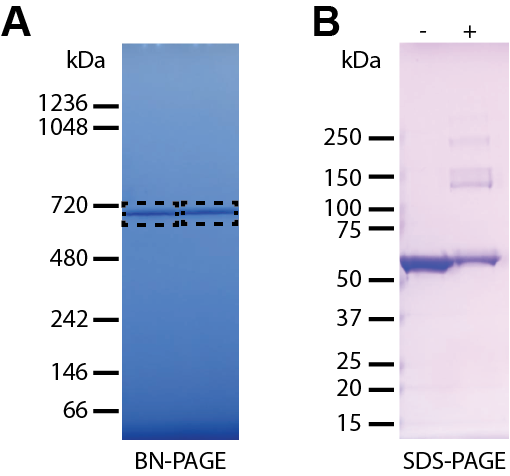
\includegraphics[]{Chapter.2/Figures/SI_Figure1.png} 
        \caption{\textbf{Combining BN-PAGE with IGX-MS.} \textbf{A.} BN-PAGE of E. Coli (10 $\mu$g). Respective bands (dashed boxes) were excised and incubated with or without the cross-linker DSS (1.5 mM). \textbf{B.} SDS-PAGE of GroEL, extracted from respective gel band (see A). The non-cross-linked control (-) showed only a band at 57 kDa of the GroEL subunit, whereas the DSS-cross-linked sample (+) reveals several bands at higher Mw.}
        \label{fig:ch2_app_fig1}
    \end{figure*}

    \vspace{1cm}

    \begin{figure*}[hbt!]
        \center
        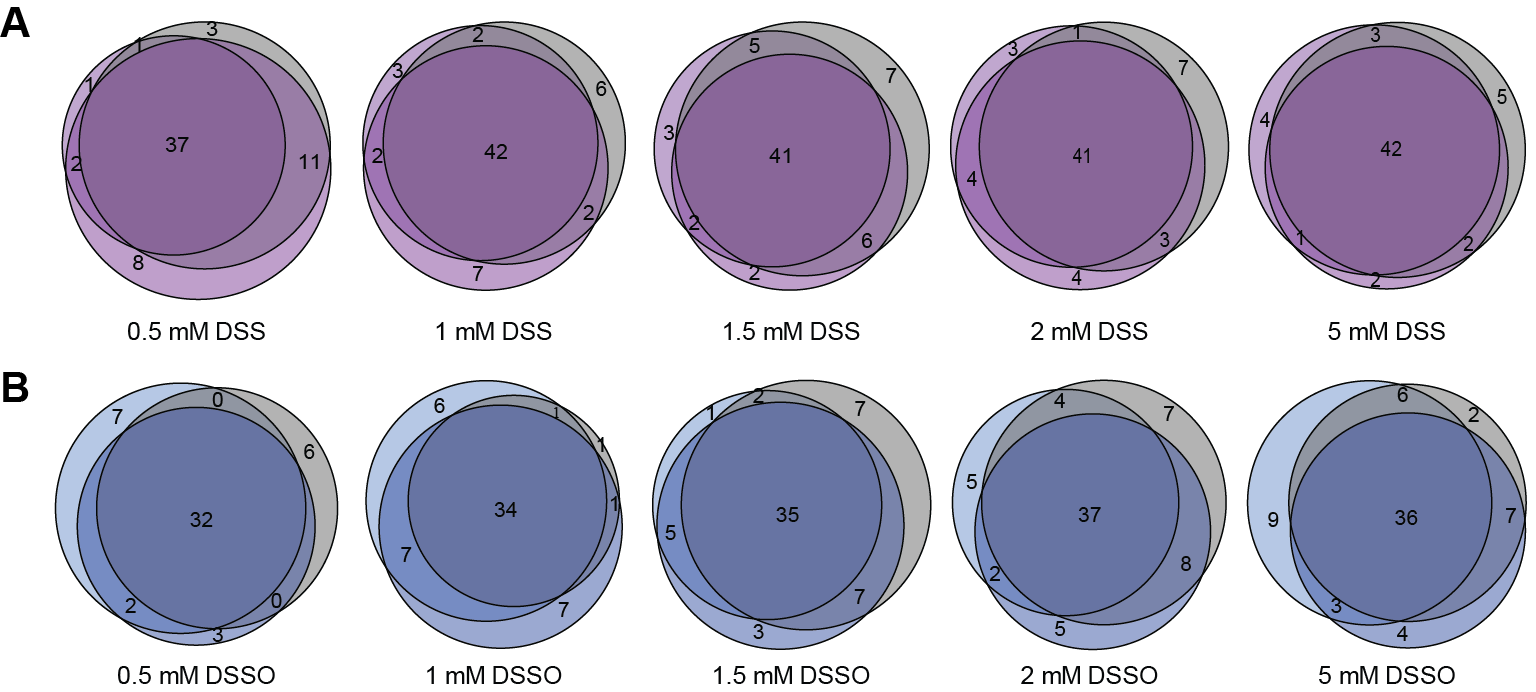
\includegraphics[]{Chapter.2/Figures/SI_Figure2.png} 
        \caption{\textbf{In-gel cross-linking is highly reproducible and only marginally dependent on the concentration of the reagent.} \textbf{A.} Venn diagrams displaying the overlap of detected unique cross-links in triplicate measurements of GroEL cross-linked in gel with different DSS concentrations. \textbf{B.} Venn diagrams displaying the overlap of detected unique cross-links in triplicate measurements of GroEL cross-linked in gel with different DSSO concentrations.}
        \label{fig:ch2_app_fig2}
    \end{figure*}

    \clearpage

    \begin{figure*}[hbt!]
        \center
        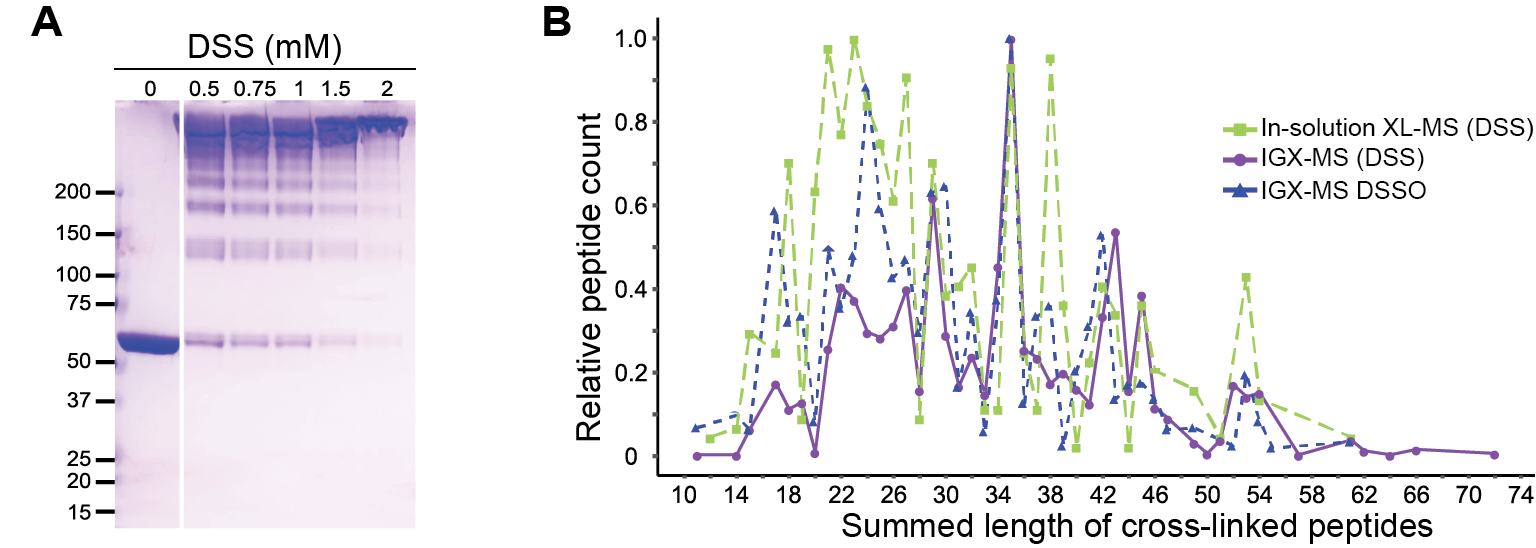
\includegraphics[]{Chapter.2/Figures/SI_Figure3.png} 
        \caption{\textbf{Optimization of cross-linker concentration for in-solution XL-MS and observed cross-linked peptide length distributions for IGX-MS and in-solution XL-MS.} \textbf{A.} GroEL was cross-linked in-solution using different DSS concentrations for the optimization of the cross- linker concentration. The samples were then loaded onto a SDS-PAGE for visualization. A concentration of
        0.75 mM DSS was selected for further experiments. \textbf{B.} Comparison of summed length of cross-linked peptide-pairs from IGX-MS (1.5 mM DSS or 2 mM DSSO) or in-solution XL-MS (0.75 mM DSS) experiments.}
        \label{fig:ch2_app_fig3}
    \end{figure*}

    \begin{figure*}[hbt!]
        \center
        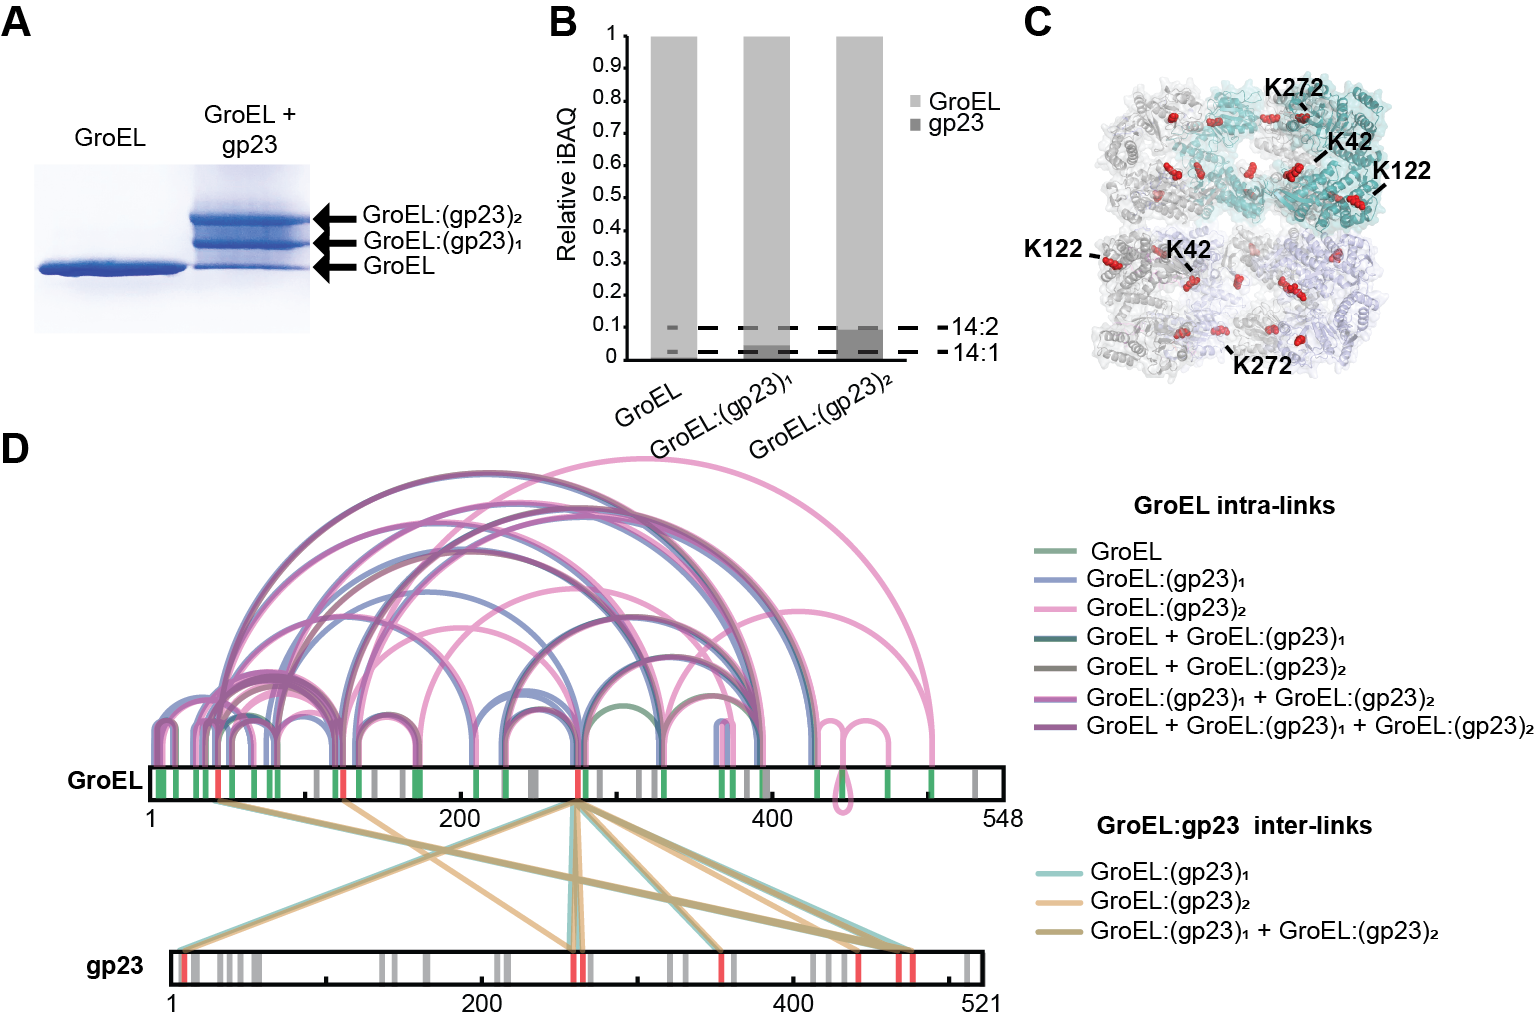
\includegraphics[]{Chapter.2/Figures/SI_Figure4.png} 
        \caption{\textbf{IGX-MS of GroEL bound to the gp23 substrate.} \textbf{A.} BN-PAGE of GroEL incubated with or without unfolded gp23. The arrows indicate free GroEL or GroEL bound to one or two molecules of gp23. \textbf{B.} Label-free quantification for the estimation of the stoichiometry of the formed complexes. Relative iBAQ values of GroEL and gp23 in the three bands. Dashed lines indicate the GroEL:gp23 ratios for the theoretically expected 14:1 and 14:2 ratios. \textbf{C.} Cross-section of the structural model of GroEL (PDB ID: 1KP8) with lysine residues that were found to be cross-linked to gp23 shown in red spheres. \textbf{D.} Overlay of cross-links identified in the three bands, representing the GroEL, the GroEL:gp23, and GroEL:(gp23)2 complex. GroEL intra-links are colored green, purple, and pink. Inter-links are colored turquoise and sand. For clarity, intra-links in gp23 are not depicted. Grey lines in the sequence indicate lysine residues not cross-linked, red lines indicate inter-linked lysine residues, and green lines indicate intra-linked residues.}
        \label{fig:ch2_app_fig4}
    \end{figure*}

    \begin{figure*}[hb!]
        \center
        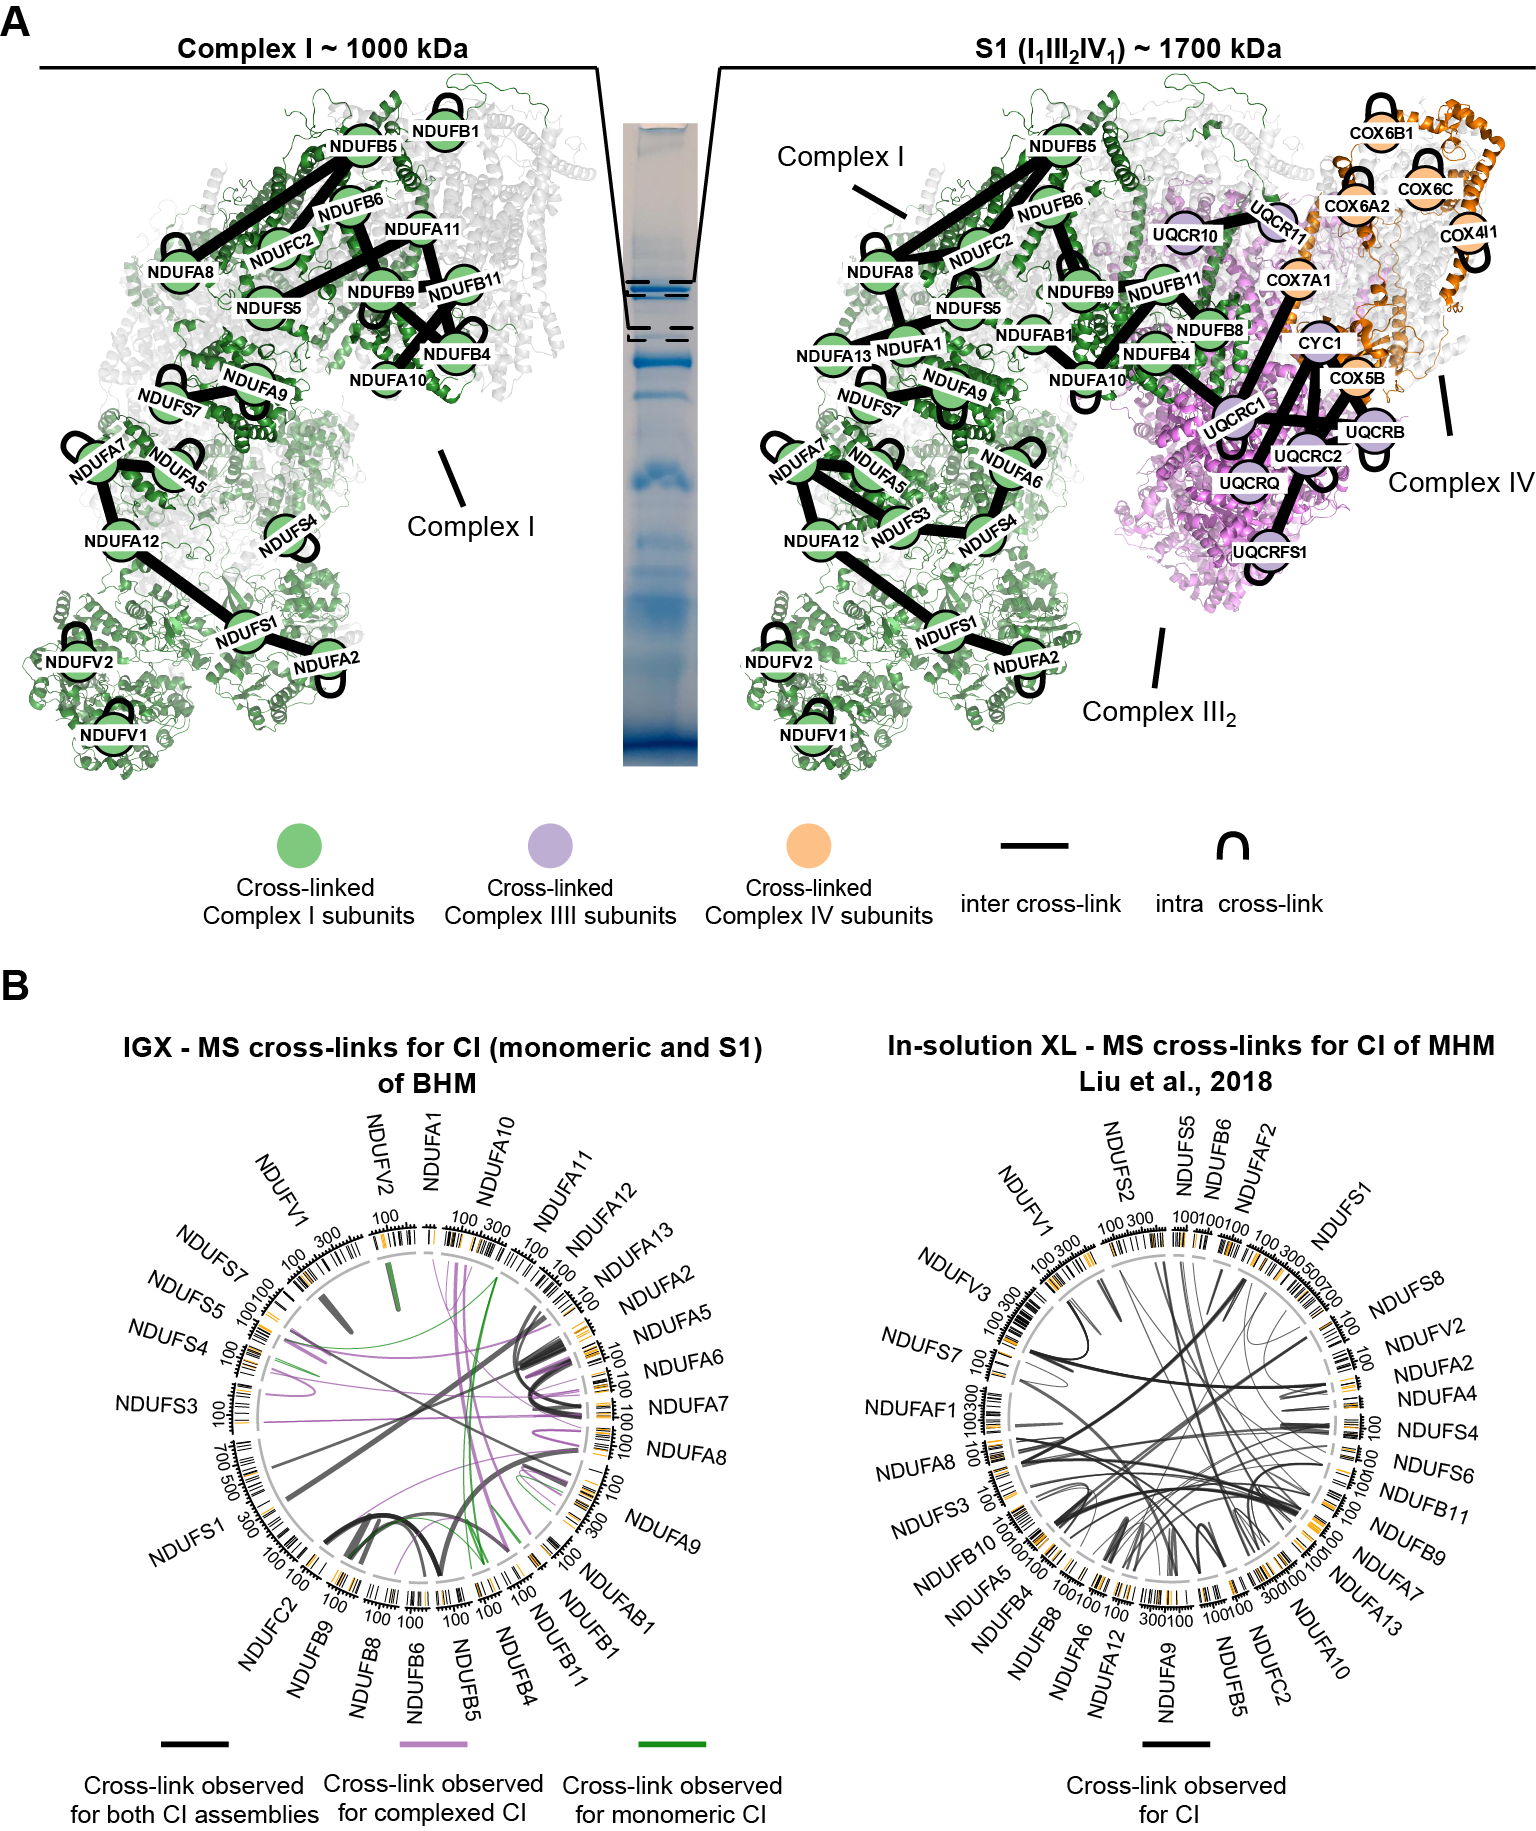
\includegraphics[]{Chapter.2/Figures/EV_Figure1.png} 
        \caption{}
        \label{fig:ch2_app_fig5}
    \end{figure*}

    \addtocounter{figure}{-1}
    \begin{figure*}[ht!]
        \caption{\textbf{Assembly state specific cross-linking of Complex I from bovine heart mitochondria (BHM) in its monomeric state and when incorporated within a super-complex by IGX-MS.} \textbf{A.} IGX-MS cross-links observed within monomeric complex I (left) - and when incorporated within the super complex S1 (right). Node positions are in accordance with respective subunit coordinates of the published S1 structure (PDB ID: 5GUP). \textbf{B.} Circos plots of detected cross-links within the monomeric complex I (CI) (black Gene names) identified by IGX-MS (left panel) and in-solution XL-MS (right panel). The position of the lysine residues is shown in the outer-ring, and cross-linked residues are colored dark orange. For IGX-MS generated data (left panel), cross-links are colored based on the CI assembly state they were detected for. For in-solution XL-MS (right panel) the cross-links originated from a mixture of all assembly states of CI present in-solution. Thickness of the cross-link lines correlates to the number of detected cross-linked spectra matches (CSMs).}
    \end{figure*}

    \begin{figure*}[hbt!]
        \center
        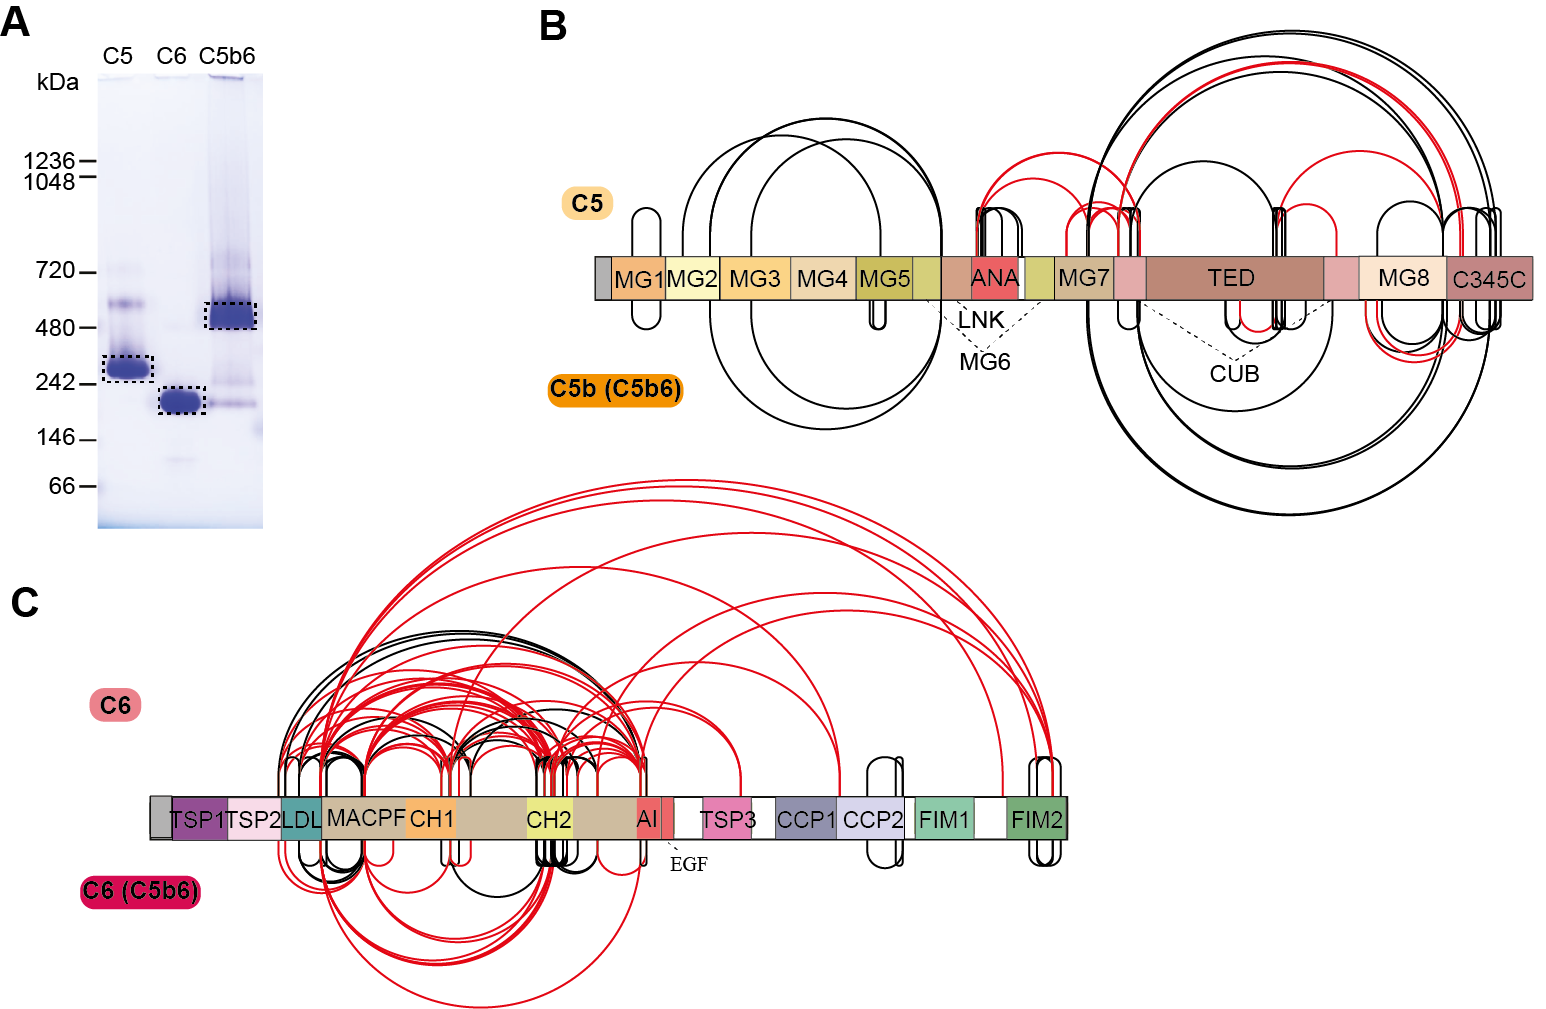
\includegraphics[]{Chapter.2/Figures/SI_Figure5.png} 
        \caption{\textbf{IGX-MS of C5, C6, and C5b6.} \textbf{A.} BN-PAGE of complement components C5, C6, and the C5b6 complex. For each lane 5 $\mu$g of protein (C5, C6), respectively 10 $\mu$g (C5b6) of protein, were applied onto the gel. Dashed boxes indicate the bands cut out for subsequent IGX-MS analysis. \textbf{B-C.} Schematic overview for domain-centered cross-link results for C5 and Cb5b in the C5b6 complex (B) or C6 and C6 in the C5b6 complex (C). Black lines indicate cross-links within the distance restraints ($\leq$ 30 Å). Red lines indicate cross-links exceeding the distance restraints ($\geq$ 30 Å). Notably, for C6, many cross-links to the N-terminal domains are not present when C6 is complexed to C5b.}
        \label{fig:ch2_app_fig6}
    \end{figure*}

    \begin{figure*}[hbt!]
        \center
        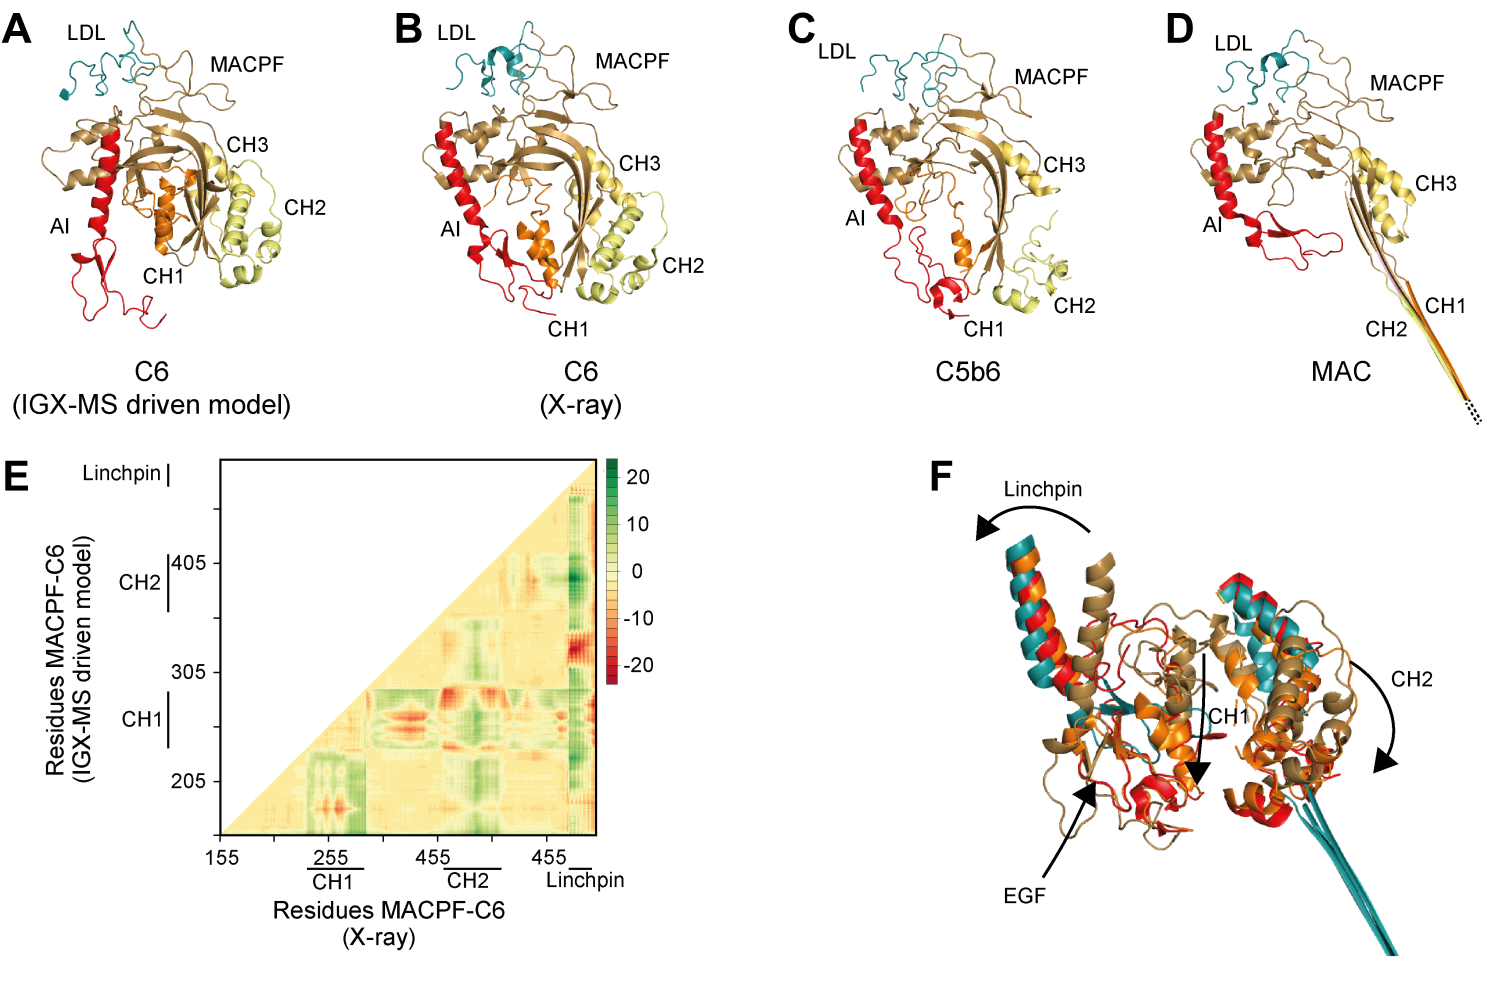
\includegraphics[]{Chapter.2/Figures/EV_Figure2.png} 
        \caption{\textbf{Structural rearrangements of the AI and CH regions of C6 when going from free C6, the C5b6 intermediate structure to C6 in the fully assembled MAC.} \textbf{A-D.} Cartoon representation of the LDL (deepcyan) and MACPF (sand) domains within the IGX-MS driven C6 model (A), C6 from the X-ray structure (PDB ID: 3T5O) (B), C6 complexed with C5b (PDB ID: 4A5W) (C), and C6 as part of the MAC (PDB ID: 6H03) (D). The regions CH 1-3 (orange, paleyellow, and yelloworange) and auto-inhibitory (AI, red) within MACPF are shown. \textbf{E.} The difference distance matrix of superposed C6-MACPF domains. The difference distance was calculated by substracting the coordinates of aligned MACPF backbones of the IGX-MS driven model and the I-tasser model (for complete sequence coverage) of C6 -X-ray structure (PDB ID: 3T5O). The distance values are plotted with colors representing C$\alpha$ differences of -20 to 20 Å according to the right-sided scale. \textbf{F.} Overlay of the AI (composed of linchpin helix and EGF domain), CH1, and CH2 regions of MACPF in four distinct conformations of C6, namely the IGX-MS driven model (sand), the deposited C6 X-ray structure (orange), when incorporated in the C5b6 complex (red), and finally when incorporated in the fully assembled MAC (deepcyan). Arrows indicate the conformational changes of the different regions from free C6 (IGX-MS driven model) to partial activation (PDB ID: 3T5O) and C5b binding (PDB ID: 4A5W) and final assembly into the MAC (PDB ID: 6H03).}
        \label{fig:ch2_app_fig7}
    \end{figure*}

    \begin{figure*}[hbt!]
        \center
        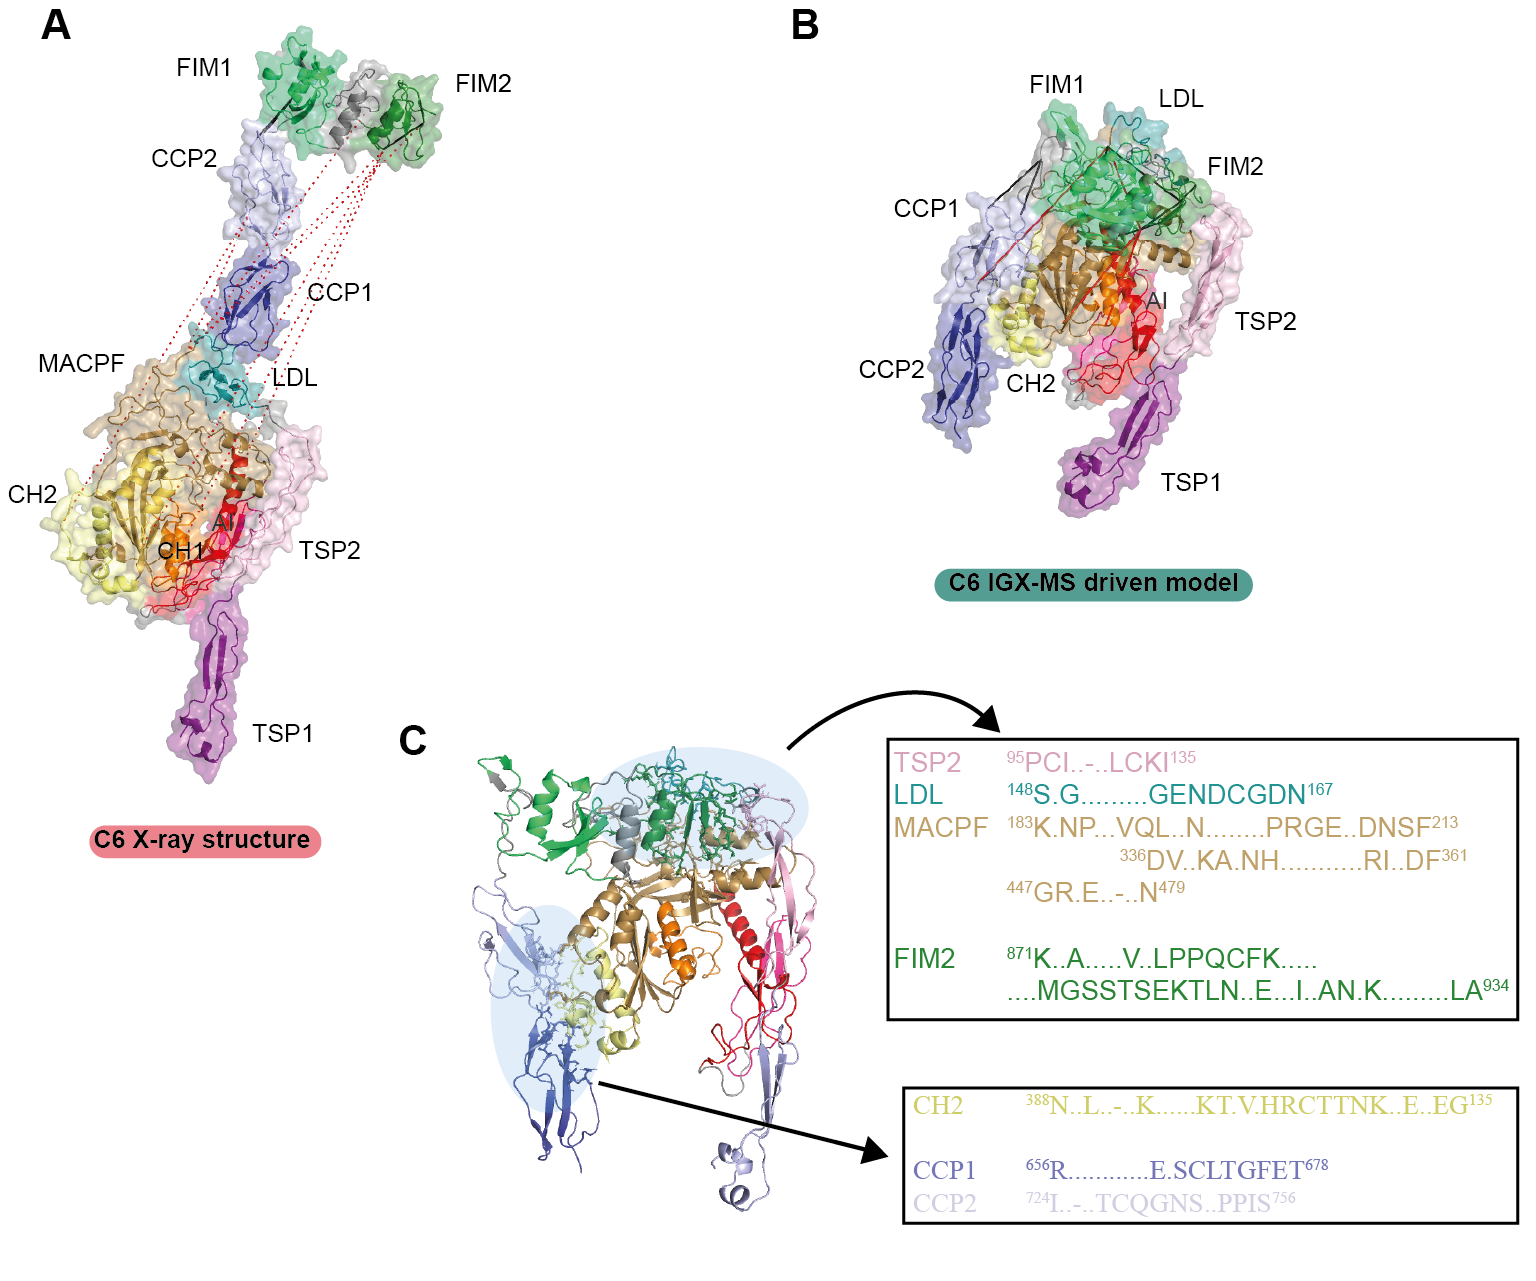
\includegraphics[]{Chapter.2/Figures/SI_Figure6.png} 
        \caption{\textbf{Comparison of the monomeric C6 X-ray structure and IGX-MS driven structural model, wherein the C5b-binding region becomes docked to the main body.} \textbf{A.} Cross-links identified for residues in the C5b-binding region plotted onto the C6 X-ray structure (PDB ID: 3T5O). Cross-links that were used to dock the C5b-binding domain (CCP1-2, FIM1-2) to the LDL- and MACPF domain are shown as dotted lines. Black lines indicate cross-links within the distance restraints ($\leq$ 30 Å). Red lines indicate cross-links exceeding the distance restraints ($\geq$30 Å). \textbf{B.} IGX-MS driven structural model of free C6. Cross-links obtained for the C5b-binding region are plotted onto the final model of C6. Solid black lines indicate distances below 30 Å, and red dotted lines indicate links with a distance larger than 30 Å. \textbf{C.} Interaction interface analysis for C5b-binding and the LDL-, MACPF domains. Blue circles indicate binding interfaces, for which interacting residues were identified (shown as sticks). The identified interacting residues of the different domains are shown in the black boxes.}
        \label{fig:ch2_app_fig8}
    \end{figure*}

    \begin{figure*}[hbt!]
        \center
        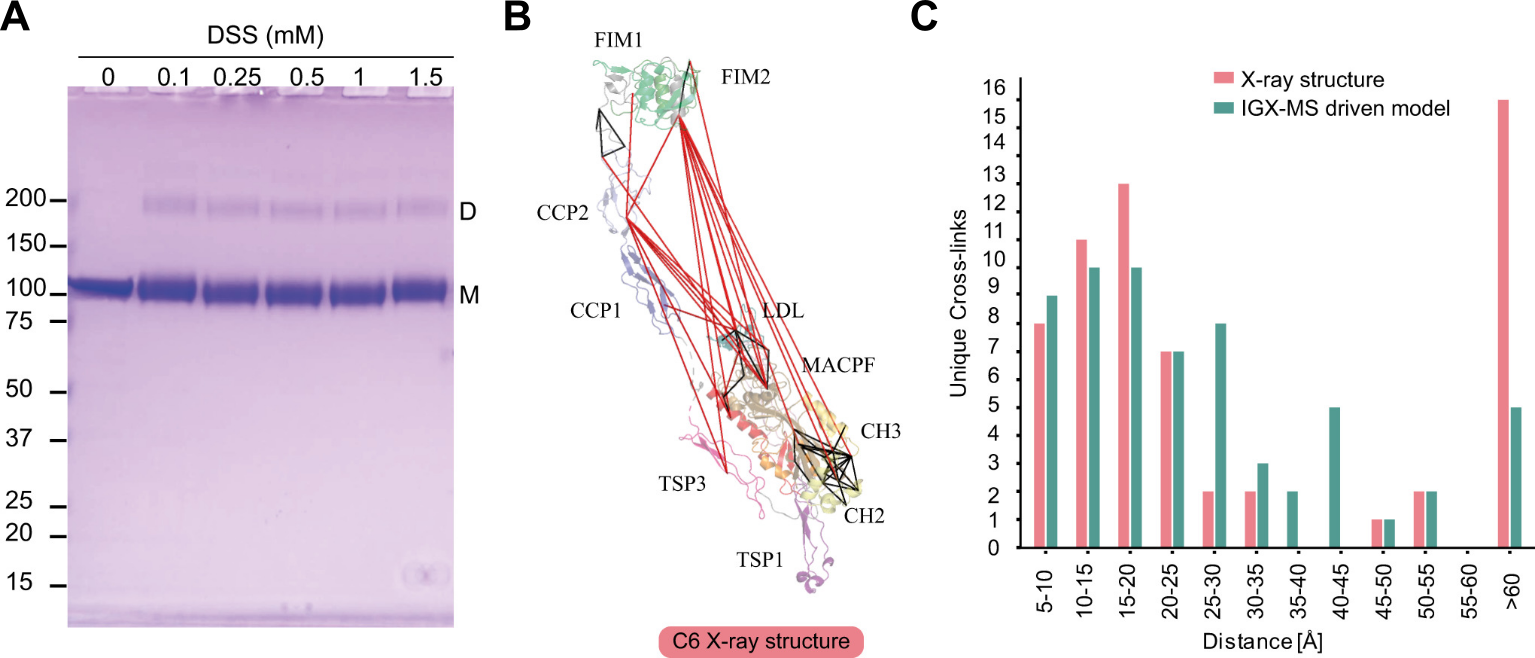
\includegraphics[]{Chapter.2/Figures/EV_Figure3.png} 
        \caption{\textbf{In-solution XL-MS of C6.} \textbf{A.} DSS concentration optimization for cross-linking C6 in-solution monitored by SDS-PAGE. The upper band ($\sim$200 kDa) indicates a C6 dimer that is formed upon cross-linking whereas the more abundant lower band ($\sim$100 kDa) represents monomeric C6. \textbf{B.} Obtained cross-links for monomeric C6 plotted on the available X-ray structure of C6 (PDB ID: 3T5O). The red lines indicate distances > 30 Å. The different domains of C6 are indicated in black. \textbf{C.} Distribution of lysine C$\alpha$-C$\alpha$ distances of unique cross-links identified by in-solution XL-MS for monomeric C6 when plotted on the reported X-ray structure (pink bars, PDB ID: 3T5O) and the IGX-MS driven refined structural model (green bars). The average distance of all cross-links is 41.7 Å when using the X-ray structure which reduces to 26.2 Å for the IGX-MS driven structural model.}
        \label{fig:ch2_app_fig9}
    \end{figure*}

    \begin{figure*}[hbt!]
        \center
        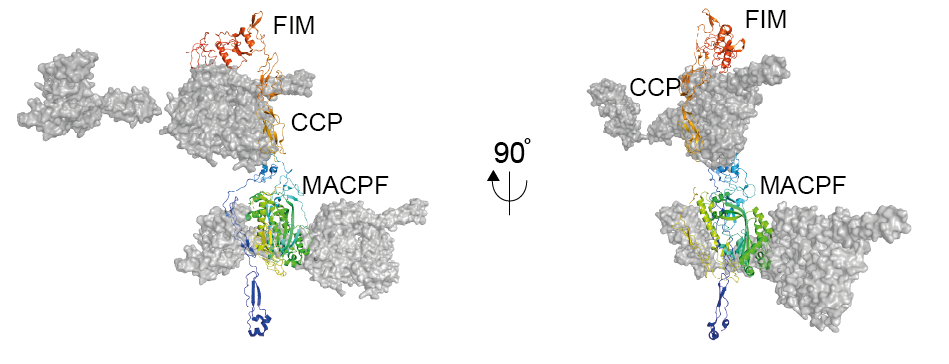
\includegraphics[]{Chapter.2/Figures/SI_Figure7.png} 
        \caption{\textbf{Possible interactions between adjacent C6 molecules in the deposited X-ray crystal structure.} The total electron density acquired for the X-ray structure of C6 (PDB ID: 3T5O) reveals closely packed neighboring C6 molecules. A single C6 molecule is shown here in a rainbow-colored cartoon in two orientations. The surface (grey) of two adjacent C6 molecules in the electron density maps shows the interaction of the C-terminal CCP and FIM domains of one C6 molecule with the MACPF domain of another C6 molecule.}
        \label{fig:ch2_app_fig10}
    \end{figure*}

\end{subappendices}

\clearpage
\section*{References}
\bibliographystyle{Style_settings/bibstyle_pnas}
\bibliography{Chapter.2/chapter2_bib_form}
%\picturechapter{Molecular characterization of a complex of apoptosis-inducing factor 1 with cytochrome \emph{c} oxidase of the mitochondrial respiratory chain}{Chapter.1/Figures/chapterpage.pdf} \label{ch-3}
\vspace*{0.25cm}

\footnotesize Johannes F. Hevler, Riccardo Zenezeni Chiozzi, Alfredo Cabrera-Orefic, Ulrich Brandt, Susanne Arnold and Albert J.R. Heck
%
\begin{center}
	\vspace{1.125cm}
	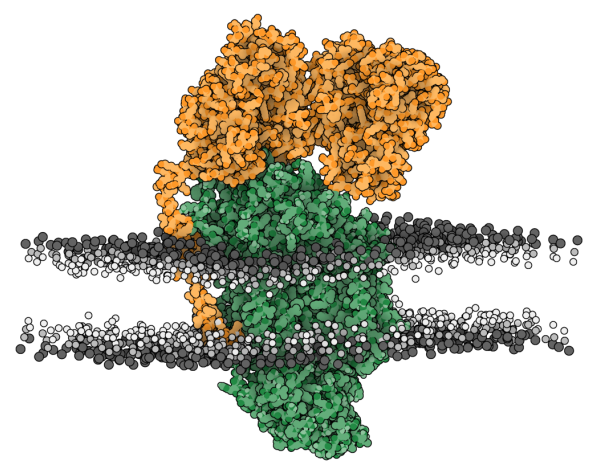
\includegraphics[width=0.7\textwidth]{Chapter.3/Figures/COX_AIFM1_Goodshell_like.png}
	\vspace{0.25cm}
\end{center}
%
\begin{flushleft}
	\vspace*{\fill}
	\rule{\textwidth}{1pt}\\[0cm]
	\textbf{This chapter is based on work in the following publication:}\\
	\footnotesize
	\textbf{\emph{PNAS}} (2021), 118:e2106950118, doi:10.1073/pnas.2106950118\\
	\footnotesize
\end{flushleft}
%%Abstract
\begin{abstract102}
	Combining mass spectrometry based chemical cross-linking and complexome profiling, we analyzed the interactome of heart mitochondria. We focused on complexes of oxidative phosphorylation and found that dimeric apoptosis inducing factor 1 (AIFM1) forms a defined complex with $\sim$10\% of monomeric cytochrome \emph{c} oxidase (COX), but hardly interacts with respiratory chain supercomplexes. Multiple AIFM1 inter-cross-links engaging six different COX subunits provided structural restraints to build a detailed atomic model of the COX-AIFM1\textsubscript{2} complex (PDBDEV\_00000092). Application of two complementary proteomic approaches thus provided unexpected insight into the macromolecular organization of the mitochondrial complexome. Our structural model excludes direct electron transfer between AIFM1 and COX. Notably however, the binding site of cytochrome \emph{c} remains accessible allowing formation of a ternary complex. The discovery of the previously overlooked COX-AIFM1\textsubscript{2} complex and clues provided by the structural model hint at potential roles of AIFM1 in OXPHOS biogenesis and in programmed cell death.
\end{abstract102}
%%Main Text
\section{Introduction}
\lettrine[lraise=0.1, nindent=0em, slope=-.5em]{M}{itochondria} are considered the powerhouse of aerobic eukaryotic cells, as they contain the major pathways of oxidative energy metabolism and produce the bulk of ATP by oxidative phosphorylation (OXPHOS) necessary for cellular homeostasis. Only at the end of the last century it became evident that mitochondria also are key players in apoptosis and that this process is tightly linked to OXPHOS components \cite{RN1}. Apoptosis Inducing Factor (AIFM1) was one of the proteins found to be released from the mitochondrial intermembrane space during programmed cell death and to have the capacity to induce chromatin condensation and DNA fragmentation in a caspase-independent fashion \cite{RN2}. A mutation found in AIFM1 has been associated with Cowchock syndrome (OMIM 310490) \cite{RN3}. Early on, it was also reported that ablation of AIFM1 leads to OXPHOS deficiency \cite{RN4}, in line with findings that AIFM1 mutations cause combined oxidative phosphorylation deficiency 6, a severe mitochondrial encephalomyopathy (OMIM 300816; \cite{RN5}). More recently, it has been proposed that AIFM1 is involved in the disulfide relay of the mitochondrial intermembrane space by serving as import receptor of CHCHD4/MIA40 \cite{RN8, RN7, RN6}. However, the specific mechanisms and molecular interactions by which these different functions of AIFM1 are connected in health and disease are not well resolved. For example, AIFM1 deficiency affects OXPHOS predominantly by lowering the amount of respiratory chain complex I \cite{RN4}. Other components were found to be affected in a tissue specific manner. In AIFM1 deficient patients \cite{RN5}, ablation of AIFM1 in skeletal and heart muscle affected cytochrome \emph{c} oxidase (COX) in addition to complex I, whereas in liver, deficiency of complexes I and V was observed \cite{RN10, RN9}.

In the present study, we explored the molecular interactions of AIFM1 with the multiprotein complexes of the OXPHOS system in heart mitochondria using our recently established complementary experimental approach \cite{RN11} that combines cross-linking mass-spectrometry (XL-MS) and complexome profiling (\textbf{\autoref{fig:ch3_fig1}}). To increase the depth and confidence of the study, bovine heart mitochondrial membranes (BHM) were treated with three different chemical cross-linkers: DSSO \cite{RN12}, PhoX \cite{RN13} and DMTMM \cite{RN14}. While DSSO and PhoX predominantly generate lysine-lysine residue cross-links, DMTMM acts as a condensation reagent of acidic side chains of aspartic or glutamic acids with lysine side chains, resulting in the formation of a stable bond between those residues. We found that a significant fraction of AIFM1 in its dimeric form is specifically bound to monomeric cytochrome \emph{c} oxidase, an interaction that has been overlooked so far. By using the identified cross-links as structural restraints, we generated a structural model of dimeric AIFM1 docked to monomeric COX.
\begin{figure*}[htb]
	\center
	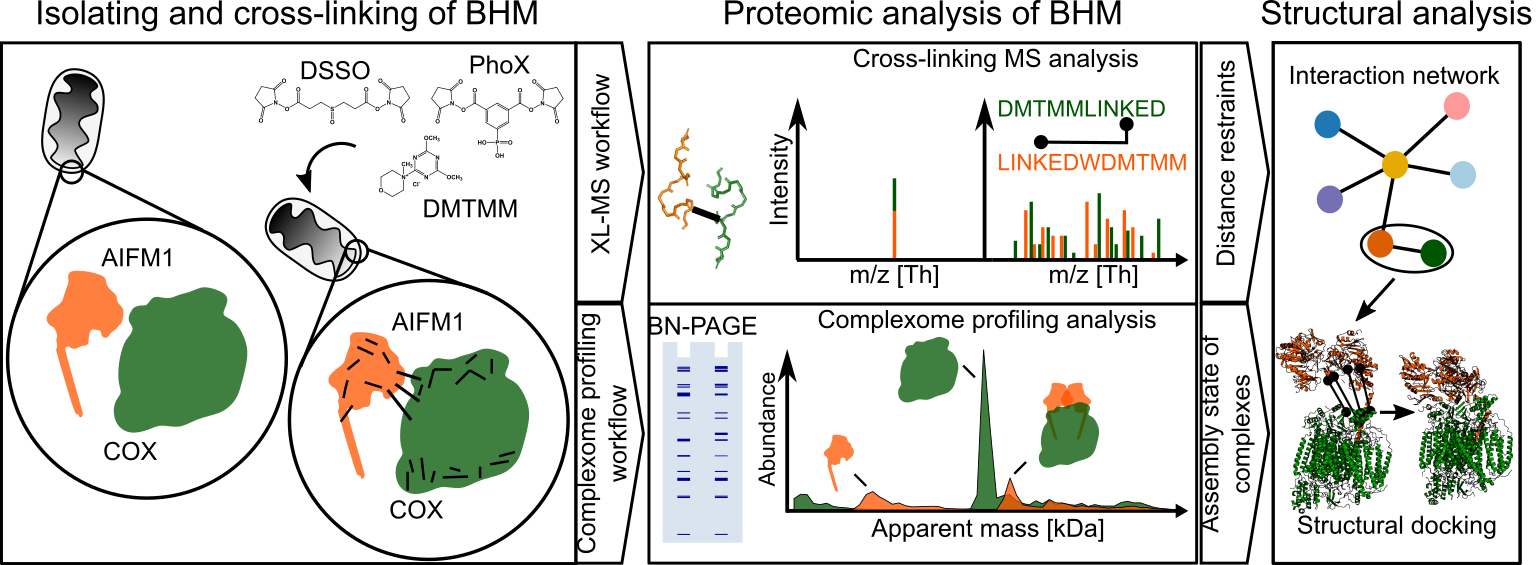
\includegraphics[]{Chapter.3/Figures/Figure1.png}
	\caption{\textbf{Two-tier experimental strategy for the analysis of proteome-wide protein-protein interactions in bovine heart mitochondria.} Mitochondria membranes were cross-linked with either of the three cross-linking reagents DSSO, PhoX or DMTMM. Subsequently, samples were analyzed by cross-linking mass spectrometry (XL-MS) and complexome profiling. Identified cross-linked peptides were used to generate protein-protein interaction networks. Protein interactions and structural models of AIFM1 with COX were then computationally modelled using the distance restraints from XL-MS data together with the assembly state and stoichiometry information obtained by complexome profiling.}
	\label{fig:ch3_fig1}
\end{figure*}
%
\section{Results and Discussion}
We analyzed the organization and interaction landscape of protein complexes in bovine heart mitochondria by combining cross-linking mass spectrometry XL-MS and complexome profiling \cite{RN15, RN11} thereby adding new information on native state multiprotein complexes of interest and expanding previous work that explored the interactome of mitochondria from different organisms, tissues and cells by XL-MS \cite{RN20, RN18, RN16, RN19, RN17}.
%
\subsection*{Exploring mitochondrial complexes by combined cross-linking and complexome profiling}
To increase the depth of the protein-interaction map of BHM we applied multiple cross-linkers (DSSO, PhoX and DMTMM). Throughout the manuscript, the term cross-link is used to describe a link between two residues coming from two unique peptides, with an intra cross-link describing a linked residue pair within a protein and an inter cross-link describing a linked residue pair between two different proteins. Additionally, identified cross-links were filtered, so that only cross-links corresponding to protein-protein interactions that were reported for at least two cross-linkers and with at least two CSMs were kept. Covering 215 proteins listed in MitoCarta 3.0 \cite{RN21}, we obtained a total of 4413 unique cross-links (3261 intra- and 1152 inter-protein cross-links; \textbf{\autoref{fig:ch3_app_fig1}A}, \textbf{Dataset S1}). In accordance with previously published studies \cite{RN23, RN22}, the abundance of detected cross-linked proteins was higher than the median of all identified proteins in the BHM sample (8.8 vs. 6.9 log\textsubscript{10} iBAQ; \textbf{\autoref{fig:ch3_app_fig1}B}). Reflecting the large number and high abundance of membrane integral multiprotein complexes and the very high protein density, especially within the inner mitochondrial membrane, $\sim$75\% of the cross-links identified involved membrane proteins (\textbf{\autoref{fig:ch3_app_fig1}C}). For the same reasons and corroborating previous studies using mouse and human mitochondria \cite{RN16, RN21, RN19, RN17} the largest number of cross-links reflected interactions between the many subunits of OXPHOS complexes and their association to supercomplexes of respiratory chain complexes I, III and IV (1431 out of 4131 cross-links; \textbf{\autoref{fig:ch3_app_fig1}D}), also called respirasomes \cite{RN24}. Further, inter domain cross-links for complex I-III and COX where in very good agreement with previously published structural models, but providing no indications for homo-dimerization (complex I, II and COX), or multimerization (complex III; \textbf{Dataset S1}). In contrast, a significant portion of inter domain cross-links for complex V showed substantially more apparent restrain violations (\textbf{Dataset S1}). Most likely, this reflected the formation of higher order ATPase assemblies involved in shaping tightly curved cristae ridges \cite{RN25, RN26, RN27}, which can also be observed in the complexome profiling data (\textbf{\autoref{fig:ch3_app_fig1}E}).

Complexome profiling analysis of untreated (i.e. non-cross-linked) BHM yielded very similar results as those obtained previously with rat heart mitochondria using the same approach \cite{RN15} showing very similar migration pattern of the OXPHOS complexes and respirasomes (\textbf{\autoref{fig:ch3_app_fig1}E}; \textbf{Dataset S2}). When the samples were cross-linked with PhoX and DMTMM before subjecting them to complexome profiling, the overall abundance of detected proteins was not affected substantially. However, it was evident from the migration profiles of OXPHOS complexes that cross-linking to some extent prevented dissociation of complex V (CV) dimers and other fragile higher order respiratory supercomplexes during native electrophoresis (\textbf{\autoref{fig:ch3_app_fig1}E}). Importantly, in most cases the apparent molecular masses of the bulk of the OXPHOS complexes were not markedly affected by cross-linking. A notable exception was complex III (CIII) in the DMTMM treated sample, where the obligatory dimer did not migrate predominantly at the predicted apparent mass of $\sim$500 kDa as in all other conditions, but appeared at $\sim$650 kDa and showed multiple peaks at higher masses. The shift of the CIII dimer to higher masses suggested that, possibly through the large hydrophilic domains of its two core subunits, this OXPHOS complex cross-linked to a much larger extent to other mitochondrial proteins than the others. The $\sim$800 kDa peak corresponds to a previously described supercomplex between one complex III dimer and one complex IV (COX) monomer \cite{RN28}. The latter was also found in untreated and PhoX cross-linked samples, but was much more pronounced after cross-linking with DMTMM. The peaks at $\sim$1100 kDa and $\sim$1300 kDa can be interpreted as dimers of complex III dimers without and with one monomer of COX, respectively.

Taken together, these results establish that classical XL-MS analysis alone and in combination with complexome profiling delivered consistent results. Separating native complexes prior to mass spectrometric analysis provided additional key information on their apparent molecular masses and multimeric state. Cross-linking them beforehand allowed for more reliable detection of more fragile assemblies that otherwise partially or completely dissociate during solubilization and/or electrophoresis.

\subsection*{A specific complex between AIFM1 dimers and COX revealed by XL-MS}
When we performed an in-depth analysis of all detected cross-links involving OXPHOS complexes in addition to engaging their canonical components themselves, one specific protein stood out: In all our XL-MS datasets combined, AIFM1 had inter cross-links with no less than six subunits of COX with 82\% of them involving COX6B1 and COX6C (\textbf{\autoref{fig:ch3_fig2}A}; \textbf{Dataset S3}). Cross-links with COX subunits accounted for 86\% of the total inter cross-links with AIFM1. Adenylate kinase 2 (AK2) and adenine nucleotide carrier isoform 1 (SLC25A4) were the only other two proteins featuring multiple inter-protein cross-links with AIFM1.

\begin{figure*}[p]
	\center
	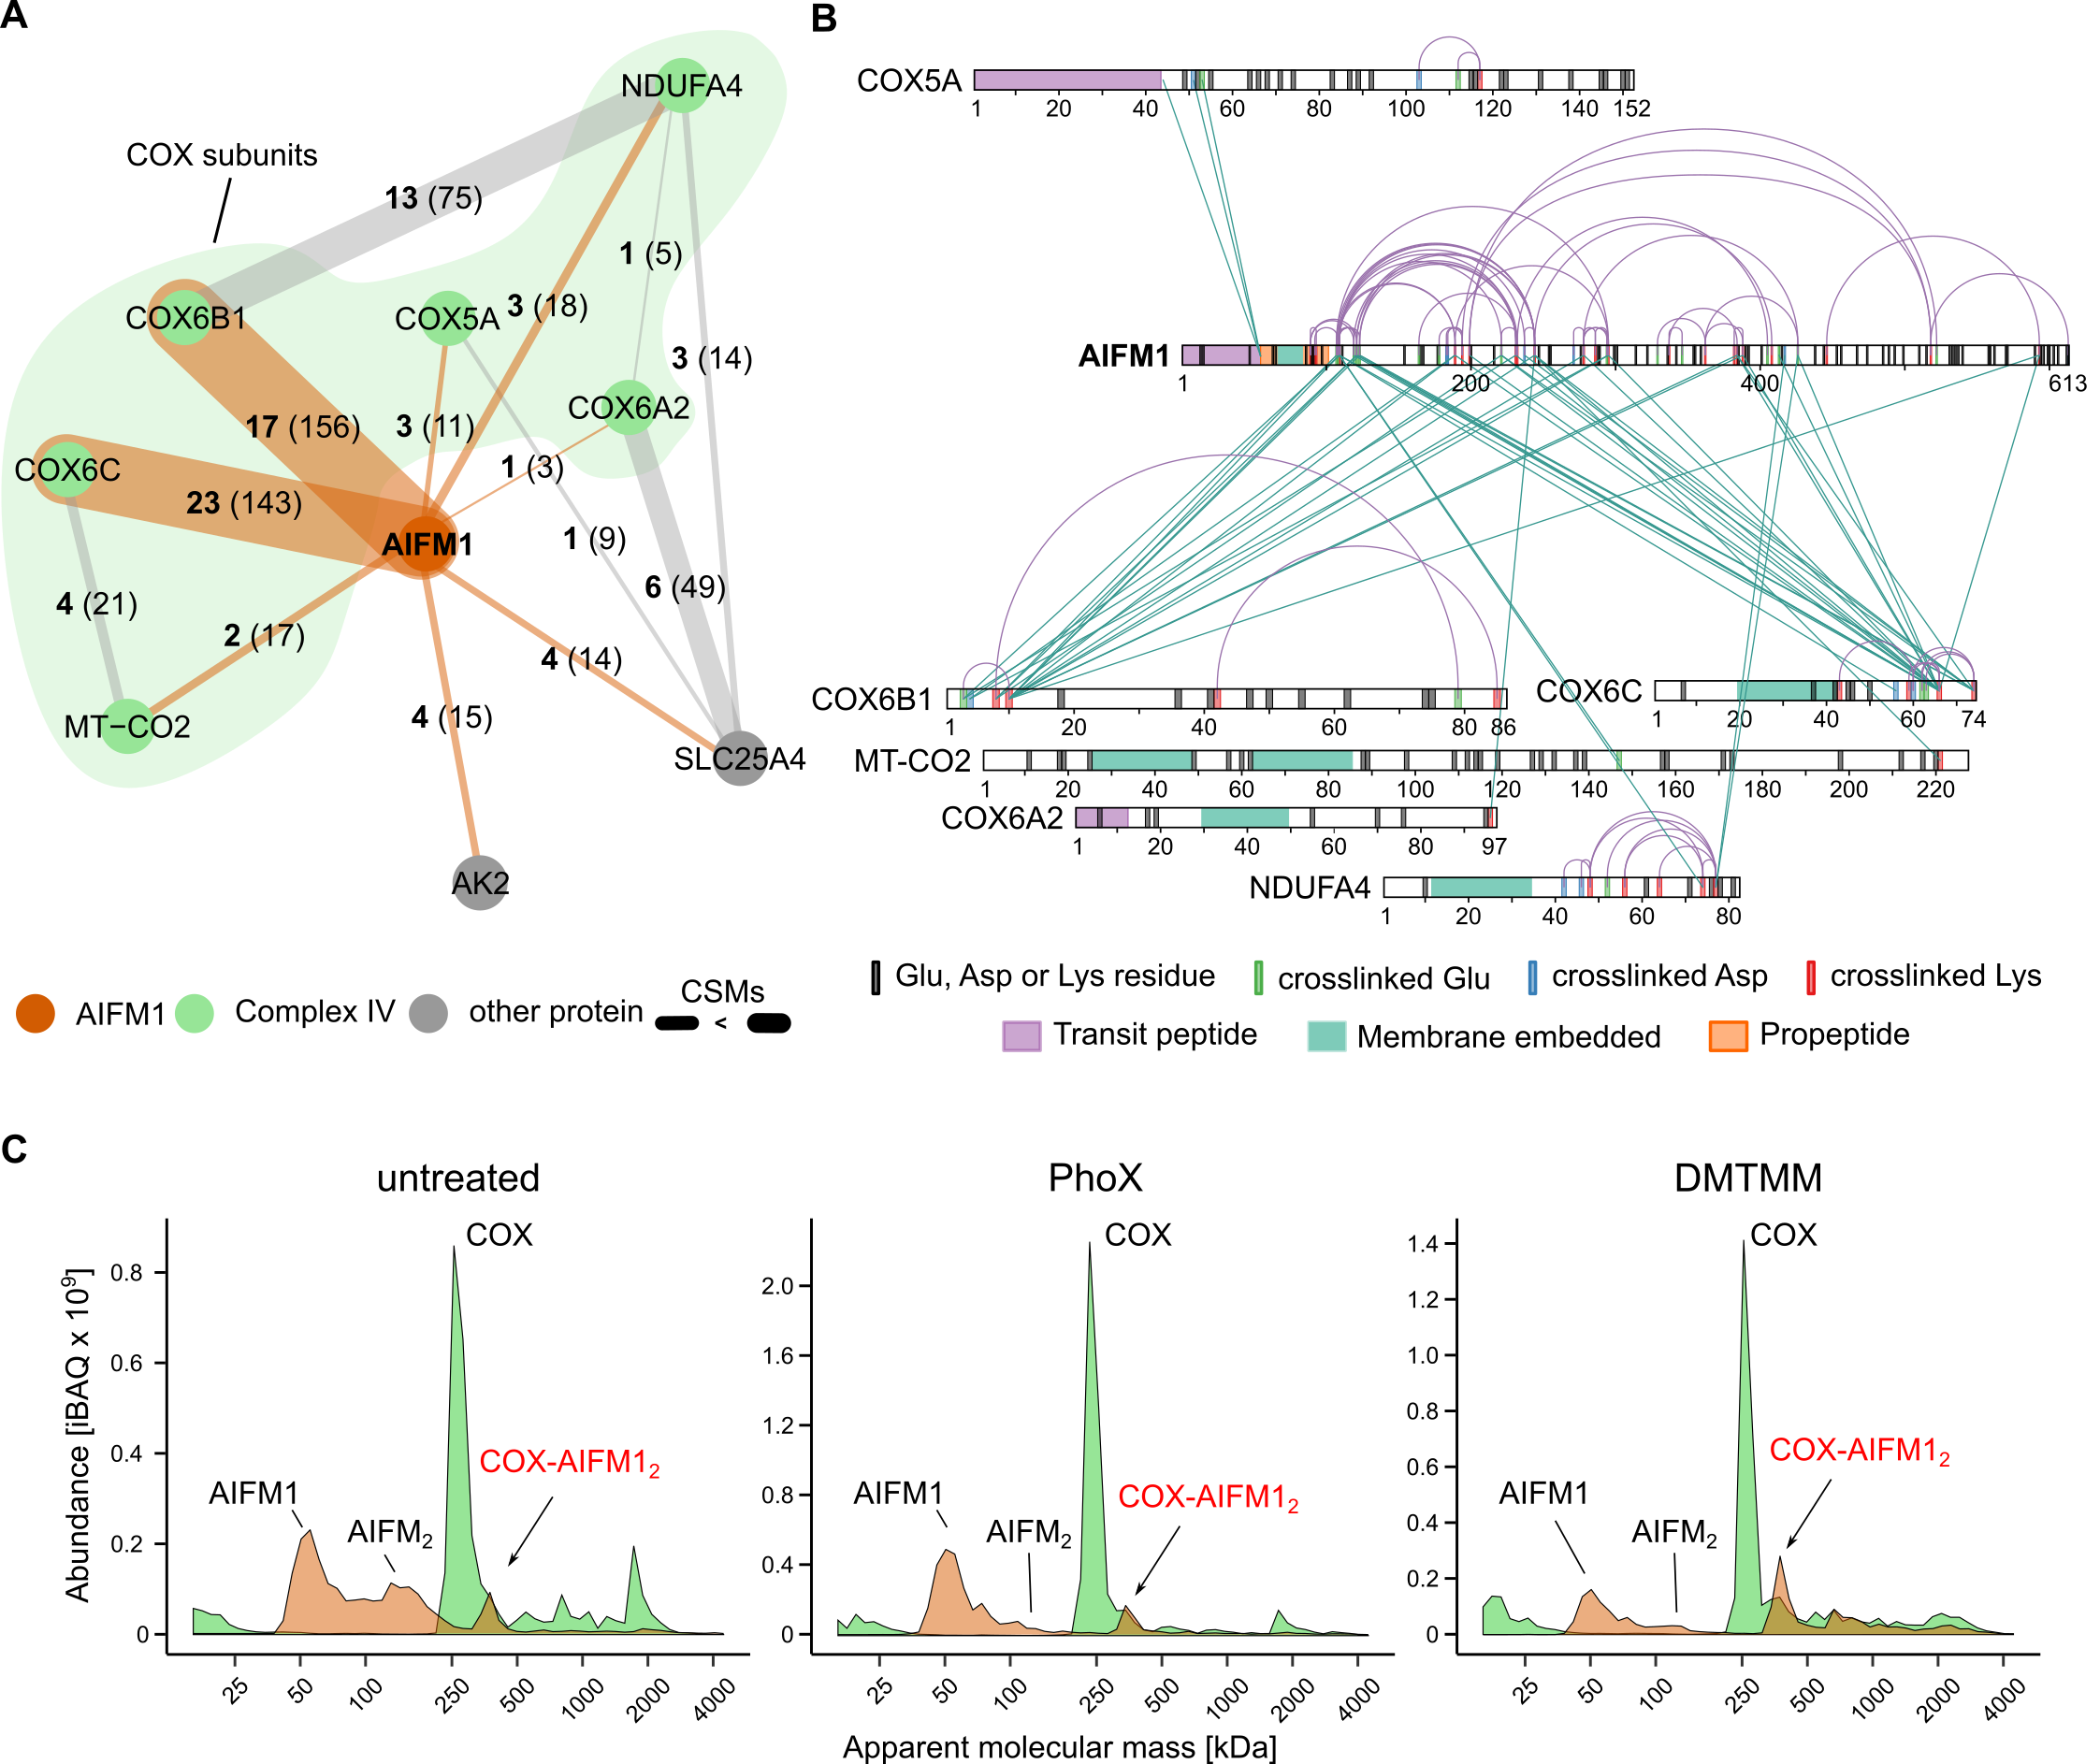
\includegraphics[]{Chapter.3/Figures/Figure2.png}
	\caption{\textbf{Dimeric AIFM1 forms a defined complex with monomeric COX.} \textbf{A.} Interaction network of AIFM1 in cross-linked BHM. Bold numbers indicate the observed cross-links for each interaction and thickness of lines indicate the cumulative evidence (CSMs) for each interaction (number in parentheses). Orange lines indicate cross-links involving AIFM1, while cross-links between AIFM1 interactors are presented as gray lines. \textbf{B.} Xi-net plot of the COX-AIFM1 interaction. Purple colored links indicate intra cross-links. Green colored links indicate inter cross-links. Respective sequence and cross-link features are indicated accordingly. \textbf{C.} Migration profiles of AIFM1 (orange) and averaged COX (green) from non-cross-linked (untreated) and cross-linked (PhoX or DMTMM) mitochondria separated by BN-PAGE (4-16\%). Peaks are annotated based on the apparent molecular mass of AIFM1 ($\sim$62 kDa) and monomeric COX ($\sim$220 kDa). In all samples, peaks corresponding to monomeric AIFM1 and COX as well as a peak corresponding to a COX-AIFM1\textsubscript{2} complex are observed. Although already present in the non-cross-linked sample, treatment with DMTMM seems to somewhat stabilize the COX-AIFM1\textsubscript{2} complex.}
	\label{fig:ch3_fig2}
\end{figure*}
The association of AIFM1 with this OXPHOS complex is remarkable in particular, since COX from bovine heart is undoubtedly the longest and best studied version of cytochrome \emph{c} oxidase \cite{RN29}. Therefore, we interrogated an earlier cross-linking dataset of mouse heart mitochondria for this interaction \cite{RN16}. Corroborating our findings, the majority of AIFM1 cross-links identified in this study engaged three different COX subunits, with COX6C being the most prominent by far (\textbf{\autoref{fig:ch3_app_fig2}A}). Of note, Liu and coworkers detected multiple cross-links between AIFM1 and AK2 as well in mouse heart mitochondria. Moreover, charting large affinity purifications-mass spectrometry (AP-MS) depositories, we found that they contained multiple instances of COX subunits interacting with AIFM1 \cite{RN30, RN32, RN31} (\textbf{Dataset S2}). Yet, buried in datasets generated by large-scale analyses of the mitochondrial interactome, these indications for AIFM1 binding to COX seem to have gone unnoticed so far.

Detailed evaluation of the observed cross-links between AIFM1 and COX (\textbf{\autoref{fig:ch3_fig2}B}; \textbf{\autoref{fig:ch3_app_fig2}B}) revealed that they were predominantly within the pyridine nucleotide-disulfide oxidoreductase domain (Pfam: PF07992; res 136-460) of AIFM1 comprising one FAD- and one NADH-binding domain. Suggesting that AIFM1 had not been cleaved to its truncated pro-apoptogenic form \cite{RN33}, additional intra- and inter-protein cross-links were observed at the N-terminal end of the pro-peptide (res 55-101) of AIFM1 that is predicted to cross the inner mitochondrial membrane (IMM) reaching to the matrix side. Notably, these cross-links were the only ones to the matrix facing subunit COX5A, while all other cross-links engaged domains of COX subunits facing the intermembrane space (IMS).

Our three independent cross-linking analyses strongly suggested that AIFM1 and COX formed a specific complex, but provided no information on the multimeric state of the interaction partners and how much of this unexpected complex was present in bovine heart mitochondria. Therefore, we applied complexome profiling to analyze complexes containing AIFM1 and COX using, the same samples as in the XL-MS analysis (\textbf{\autoref{fig:ch3_fig2}C}; \textbf{Dataset S2}). In all cases, COX was predominantly present as a monomer ($\sim$220 kDa) and a prominent fraction of AIFM1 was found to migrate at an apparent mass consistent with its monomeric state (62 kDa). Substantial amounts of AIFM1 dimers were only observed in untreated BHM indicating that they may be destabilized by the cross-linking protocol. This was possibly due to partial oxidation of NADH known to be required for AIFM1 dimerization \cite{RN8}. Importantly however, a significant amount of AIFM1 consistently showed up as a peak at an apparent mass of $\sim$350 kDa in untreated mitochondria as well as after cross-linking with PhoX or DMTMM. This peak coincided with a shoulder next to the prominent peak at $\sim$220 kDa of monomeric COX in all samples analyzed, thus suggesting the presence of a $\sim$350 kDa complex containing a dimer of AIFM1 ($\sim$124 kDa) bound to monomeric COX ($\sim$220 kDa). Notably, a shoulder on the higher mass side of the COX monomer can also be observed in complexome profiling data of human cells published earlier, but its significance was not evident at the time \cite{RN34}. Label free quantification revealed that hardly any of the other respiratory chain complexes were present in this segment of the migration profiles. In contrast, the amounts of the COX monomer and AIFM1 dimer were comparable at $\sim$350 kDa suggesting a stoichiometric association and reflecting the observations for gels with increased resolution (high range BN-gel (3-10\%); \textbf{\autoref{fig:ch3_app_fig2}C}). At the same time, no AIFM1 co-migrated with the bulk of monomeric COX at $\sim$220 kDa (\textbf{\autoref{fig:ch3_app_fig2}D}). Notably, only small amounts of AIFM1 were detected at $\sim$1,850 kDa, the predicted mass of supercomplex S1 (I\textsubscript{1}III\textsubscript{2}IV\textsubscript{1}). This was mostly observed in the DMTMM treated sample that exerted many more inter-protein cross-links in the high mass range overall (\textbf{\autoref{fig:ch3_app_fig1}A,D}). It can be concluded that in our samples, AIFM1\textsubscript{2} was bound almost exclusively to monomeric COX and, if any, very little could be found associated with supercomplexes. Consistent with its higher cross-linking efficiency, the fraction of COX engaged in the complex with AIFM1\textsubscript{2} was somewhat higher with DMTMM than in the untreated and PhoX cross-linked samples. In fact, in untreated samples the amount of COX-AIFM1\textsubscript{2} complex was variable to some extent. This suggested that it tended to dissociate during solubilization and native electrophoresis. Such behavior has been observed previously for several less tightly associated subunits of OXPHOS complexes \cite{RN36, RN37, RN35}. Overall, we could estimate that about 10\% of monomeric COX was engaged in a fairly stable stoichiometric complex with AIFM1 dimers (\textbf{\autoref{fig:ch3_app_fig2}D}).

In summary, combination of cross-linking and complexome profiling data provided compelling evidence for the presence of a defined COX-AIFM1\textsubscript{2} complex in bovine heart mitochondria. The interaction interface was defined as involving residues of the neighboring COX6C, COX6B1, NDUFA4, COX6A2 and MT-CO2 contacting the pyridine nucleotide-disulfide oxidoreductase domain of AIFM1, and residues of COX5A interacting with the matrix facing N-terminal region of its pro-peptide.

It should be noted that cross-links between AIFM1 and the complex I subunit NDUFA8 were previously reported in a study by Liu \emph{et al.} \cite{RN16}, which may relate to the small amounts of AIFM1 found in the supercomplex range. However, inspection of the high-resolution supercomplex structure (PDB: 5XTH, \cite{RN38}) revealed that the COX subunits cross-linking to AIFM1 (COX6B1, Mt-CO2, NDUFA4, COX6C1, COX5A, COX6A2) and complex I subunit NDUFA8 are too far apart from each other to be consistent with simultaneous binding of the two OXPHOS complexes to AIFM1 within the respirasome. This is fully in line with our cross-link data and proposed model of the complex.
%
\subsection*{Creation of a cross-link guided structural model of the COX-AIFM1\textsubscript{2} complex}
Next, we aimed at building a structural model for the COX-AIFM1\textsubscript{2} complex guided by the distance restraints obtained by cross-linking, also including those involving the N-terminal sequence of AIFM1 comprising its pro-peptide sequence (res 55-101). We first derived a de novo model of this so far structurally unresolved region using trRosetta \cite{RN39} to complement a homology model of the bovine AIFM1 dimer that we derived from the human structure (PDB: 4BUR; \cite{RN40}) using Robetta \cite{RN41}. The structural model obtained for the N-terminal domain of AIFM1 agreed well with secondary structure predictions and featured three alpha-helices (res 67-88; 94-98; 105-112) of which the first is predicted to be a transmembrane segment (\textbf{\autoref{fig:ch3_app_fig3}A}). We then used restraints derived from our cross-linking data to dock this model of the bovine AIFM1 dimer to the 1.8 Å structure of COX (PDB: 1V54) \cite{RN42}. Unfortunately, this COX structure does not contain the more loosely attached NDUFA4 subunit. Therefore, we used Robetta \cite{RN41} to complement it with a homology model derived from the human NDUFA4 structure (PDB: 5Z62 chain N)  \cite{RN43}.

Mapping the cross-links onto the structural models of AIFM1\textsubscript{2} and COX respectively, revealed that the majority of cross-links were below 30 Å, with a combined mean distance of 19.1 Å for DSSO/PhoX and 20.8 Å for DMTMM cross-links (\textbf{\autoref{fig:ch3_app_fig3}B-C}; \textbf{Dataset S3}). The mean distance for DSSO and PhoX cross-links was well within the theoretical maximal range of $\sim$30 Å and $\sim$25 Å, respectively. DMTMM cross-links averaged somewhat above the theoretical maximum of $\sim$15 Å, in line with previous observations \cite{RN14}. Note, that eight cross-links for AIFM1 and ten cross-links for COX were not included in these calculations, because they involved intra cross-links from AIFM1 (res 128-613) to its de novo modelled N-terminus (res 55-124) or regions not resolved in the structural models (AIFM1 res 517-550; COX4l1 res 23-25; \textbf{\autoref{fig:ch3_app_fig3}C}).

Based on solvent accessibility and distance restraints obtained from both structures, accessible interaction interfaces between COX and the AIFM1 dimer as well as COX and the N-terminal region of AIFM1 were calculated using DisVis \cite{RN44}. While this analysis suggested that the AIFM1 dimer attaches to the intermembrane space side of COX, the predicted interaction space for the N-terminal region of one AIFM1 protomer covers the transmembrane domain at the matrix side of COX making contacts to subunits COX6B1, COX6C, MT-CO2, NDUFA4 (\textbf{\autoref{fig:ch3_fig3}A}). Scoring the interface models using the restraints imposed by the cross-linking data suggests that the COX-AIFM1\textsubscript{2} interface is mostly occupied by just one AIFM1 protomer. In agreement with this notion, cross-links suggested that only one N-terminal region, not both of the AIFM1 dimer interacted directly with COX. Therefore, the final modelling of the COX-AIFM1\textsubscript{2} complex was performed by docking just one AIFM1 protomer and one N-terminal region of AIFM1 to the COX monomer. Docking was restraint by 46 of 59 unique cross-links detected for the COX-AIFM1 interaction. Haddock \cite{RN45} generated six acceptable clusters (with negative Haddock score). One cluster (cluster 7) showed better scores (overall lowest Haddock score and i-RMSD) compared to the other clusters (\textbf{\autoref{fig:ch3_app_fig4}A}). Investigation of the individual structures of produced clusters revealed that only for structures of cluster 7 the N-terminal domain of AIFM1 was positioned in accordance with its transmembrane domain. Furthermore, structural alignment of models from cluster 7 showed high cluster precision and only differed marginally from each other (RMSD = 0.942 Å; \textbf{\autoref{fig:ch3_app_fig4}B}). Lastly, clusters were validated by mapping the used cross-link restraints on the highest scoring model of each cluster, with the structure of cluster 7 satisfying them best (\textbf{Dataset S4}).
\begin{figure*}[p]
	\center
	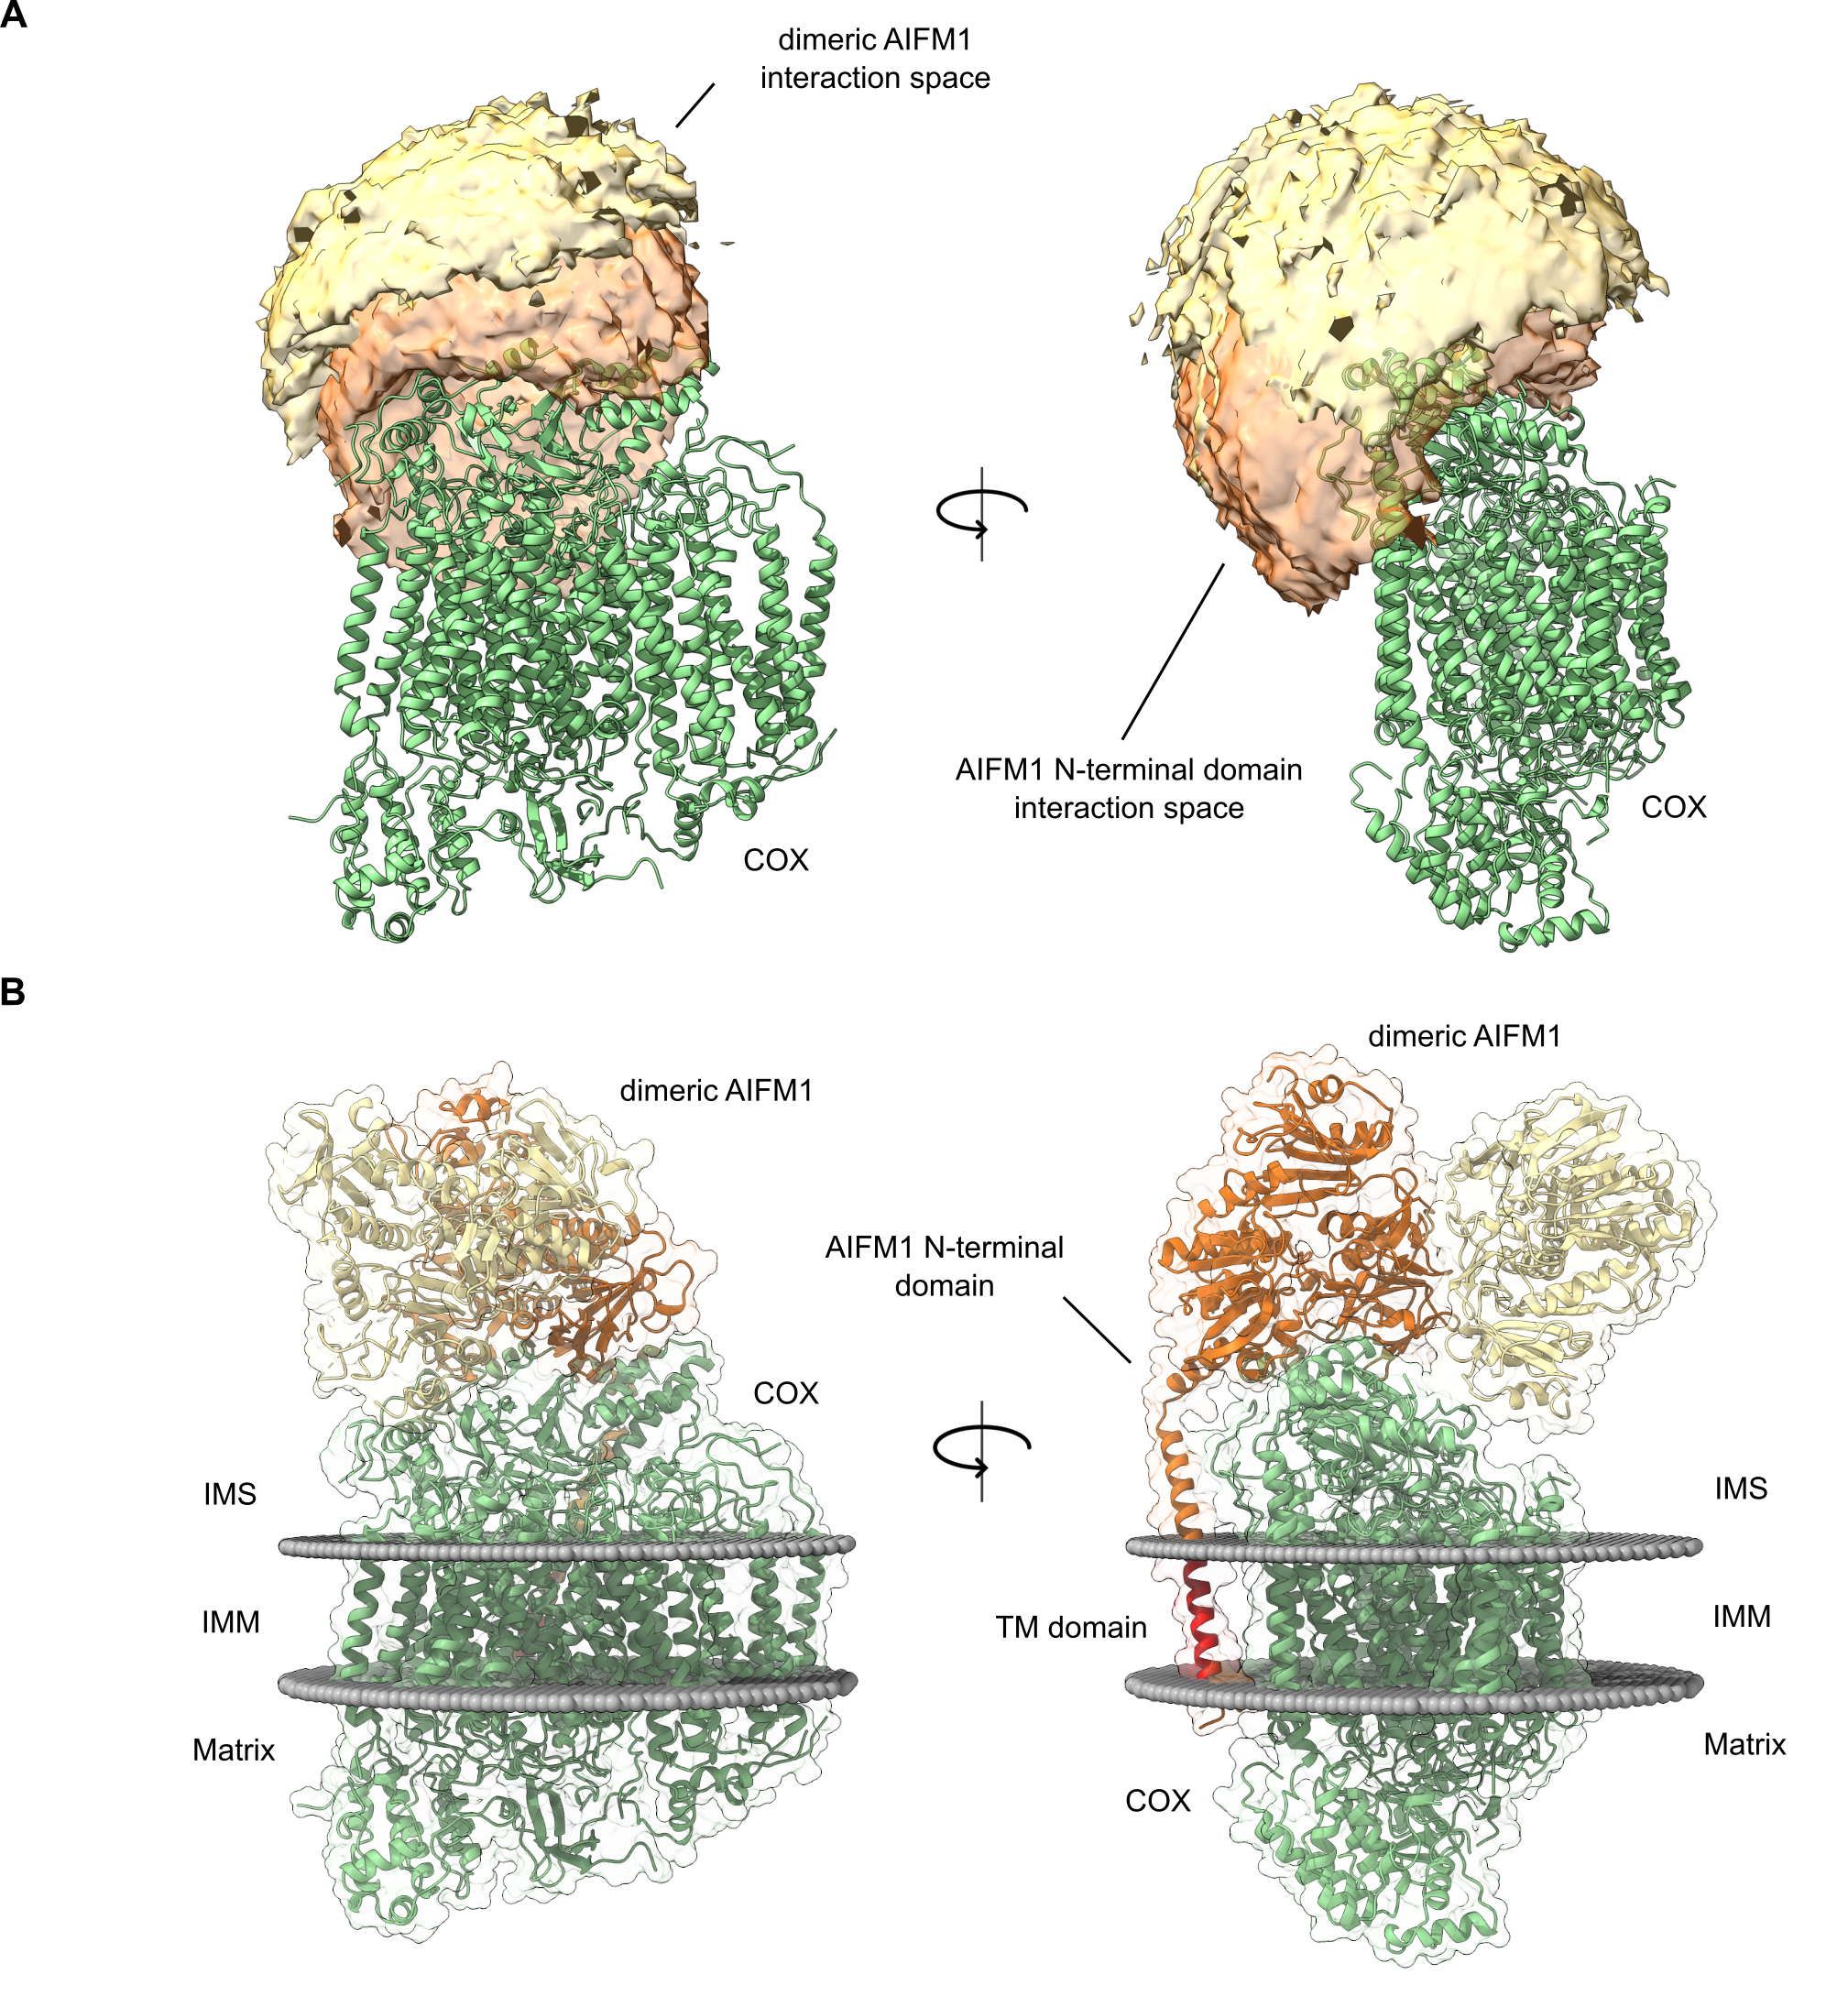
\includegraphics[]{Chapter.3/Figures/Figure3.png}
	\caption{\textbf{Cross-link derived structural model of the COX-AIFM1\textsubscript{2} complex.} \textbf{A.} Visualization of the cross-link driven accessible interaction space models for a COX-AIFM1\textsubscript{2} complex. COX is represented in green, while the bright orange volume represents the center-of-mass position of the AIFM1 dimer, and the dark orange volume represents the center-of-mass position of the model of the AIFM1-N-terminus (res 55-124). The cross-linking data are consistent with the interaction space available for docking dimeric AIFM1 and the N-terminal region of one AIFM1 protomer to monomeric COX. \textbf{B.} Cross-link derived structural model of the COX-AIFM1\textsubscript{2} complex. COX is represented in green, and AIFM1 protomers (res 128-516; 551-613 with and without N-terminal region (res 55-127) are represented in orange and yellow respectively. The transmembrane residues (67-85) of the N-terminus of the interacting AIFM1 moiety is highlighted in red. Membrane boundaries of the IMM are sketched as gray spheres. The final complex consists of monomeric COX, dimeric AIFM1 (res 128-516, 551-613) and the N-terminal region of one AIFM1 protomer (res 55-127).}
	\label{fig:ch3_fig3}
\end{figure*}
Based on overall best cluster scoring and high cluster precision, the highest scoring structure of cluster 7 was chosen as representative model for the COX-AIFM1\textsubscript{2} complex. In the final structural model of the COX-AIFM1\textsubscript{2} complex, the AIFM1 dimer “sits” on COX facing the intermembrane space side and makes contact through one AIFM1 protomer covering parts of COX6B1, COX6C1, MT-CO2 and NDUFA4 (\textbf{\autoref{fig:ch3_fig3}B}). The second AIFM1 protomer points away from COX making just one very limited contact to COX through its C-terminal loop. At the opposite side of COX, the N-terminal region of the interacting AIFM1 protomer makes contact with COX6B1 and transmembrane helices of MT-CO2 and NDUFA4 (\textbf{\autoref{fig:ch3_fig3}B}). It should be noted that after docking with Haddock, the de novo structural model covers the N-terminal region of AIFM1 only up to residue 124 creating a structurally undefined stretch of three amino acids up to residue 128, the first amino acid contained in the homology model for the main part of AIFM1. Therefore, residues 121 to 131 were re-modelled using the “Model Loops” interface in Chimera \cite{RN47, RN46}, thereby connecting the N-terminal domain to the main part of AIFM1. Cross-links (46) used for structural modelling as well as all observed cross-links (59) for COX-AIFM1\textsubscript{2} were in good agreement with the final structural model of COX-AIFM1\textsubscript{2} (\textbf{\autoref{fig:ch3_app_fig4}C-D}). The combined mean distance for DSSO/PhoX cross-links used for docking was slightly lower (26.5 Å, 20 cross-links) than for DMTMM (28.2 Å, 26 cross-links) (\textbf{Dataset S4}). Most of the obtained over length cross-links (> 33 Å, 15 cross-links) involve the N-terminal domain of AIFM1 (12 out of 15 cross-links). Interactions to the N-terminal domain are predominately mapped with DMTMM (20 out of 24 detected cross-links), explaining the slightly higher mean distance. The over length cross-links involving the AIFM1 N-terminus were obtained for cross-links to a flexible segment of COX6C (6 cross-links) and a defined residue stretch (221-244) of AIFM1 (6 cross-links) located closely to the AIFM1 N-terminus. These over length cross-links predominantly involving specific domains could indicate that cross-links are derived for several assemblies rather than one assembly, which is a challenge of in-solution XL-MS described previously \cite{RN11}. In our case, cross-links observed between AIFM1 and the AIFM1 N-terminus might well result also from monomeric or dimeric AIFM1 assemblies (\textbf{\autoref{fig:ch3_fig2}C}) potentially featuring different domain orientations as compared to AIFM1 in complex with COX. Such averaging likely explains the observed over-length cross-links. Notwithstanding these considerations, the COX-AIFM1 model is in good agreement with the cross-linking data.

Next, we performed an interaction interface analysis of the docking model that predicted three distinct interfaces between COX and AIFM1 (\textbf{\autoref{fig:ch3_fig4}A}; \textbf{Dataset S5}). The first, extensive interface is defined by the N-terminal residues of AIFM1, which interacts with neighboring residues of the COX subunits MT-CO2, NDUFA4 and COX6B1. Secondly, residues of the pyridine nucleotide-disulfide oxidoreductase domain of AIFM1 comprising the NADH- and FAD-binding domains intimately interact with MT-CO2, COX6B1 and COX6C. The third, rather small interaction interface is defined by residues of the C-terminal region of the second AIFM1 protomer and residues of MT-CO2, COX4l1 and COX7B (\textbf{\autoref{fig:ch3_fig4}B}). The interface between the hydrophilic parts of the N-terminal region of AIFM1 facing the intermembrane space is mostly driven by contacts to COX6B1 and NDUFA4, whereas its transmembrane domain predominantly interacts with one of the transmembrane segments of MT-CO2. Notably, the very N-terminal residues of AIFM1 facing the matrix side reside within a $\sim$25 Å distance from residues 44-54 of COX5A, consistent with the observed cross-links to this COX subunit (\textbf{\autoref{fig:ch3_fig2}B}).
%
\subsection*{Potential functional implications of a COX-AIFM1\textsubscript{2} complex}
While the predominant consequence of AIFM1 deficiency is impaired complex I assembly \cite{RN4}, additional COX deficiency has been reported in skeletal muscle and heart \cite{RN10, RN9}, as well as in \emph{Drosophila melanogaster} \cite{RN48} and \emph{Caenorhabditis elegans} \cite{RN49}. Conversely, AIFM1 expression was found to be significantly increased along with several COX assembly factors in human COX-negative muscle fibers \cite{RN50}. However, it seems unlikely that the COX-AIFM1\textsubscript{2} complex described here contributes to assembly or stabilization of COX, because it accounted only for 10\% or less of the total amount of this OXPHOS complex. Moreover, no apparent co-migration between AIFM1 and any of the individual COX subunits or sub-assemblies at apparent masses lower than $\sim$350 kDa was observed, suggesting that association of AIFM1 occurred only with fully assembled COX. Conditional involvement of AIFM1 in the maturation of COX assembly factors that are substrates of the disulfide relay of the intermembrane space \cite{RN8, RN7, RN6} appears as a more likely explanation for the link between AIFM1 and COX deficiency in some tissues.

It has been reported that AIFM1 is a member of the NDH-2 family of proteins \cite{RN51} and thus exhibits NADH:ubiquinone oxidoreductase activity \cite{RN52}. Nevertheless, we examined the possibility of direct electron transfer between the FAD and CuA of COX within the COX-AIFM1\textsubscript{2} complex. The minimal distance between the isoalloxazine moieties of the FADs and the CuA center was $\sim$50 Å and $\sim$55 Å (\textbf{\autoref{fig:ch3_app_fig5}}), which is more than three-times larger than the 14 Å considered as the maximum distance for efficient electron tunneling in a protein matrix \cite{RN53}. It would be conceivable that this distance is bridged by cytochrome \emph{c} (CytC) serving as an electron shuttle between AIFM1 and COX. Therefore, we explored whether cytochrome \emph{c} could still bind to its substrate binding site in the COX-AIFM1\textsubscript{2} complex. Merging our structural model with a previously obtained model of cytochrome \emph{c} bound to COX from bovine heart \cite{RN54} suggested that the AIFM1 dimer does not hamper cytochrome \emph{c} from binding to COX (\textbf{\autoref{fig:ch3_fig4}C}). However, distances of $\sim$45 Å and $\sim$47 Å between the heme moiety of cytochrome \emph{c} and the isoalloxazine rings of FAD in both AIFM1 protomers excluded direct electron transfer also in the presence of the additional heme. Yet, a substrate channeling mechanism could still be imaginable implying movement of cytochrome \emph{c} forth and back between AIFM1 and COX without leaving the complex. A crevice in the second AIFM1 protomer facing COX could potentially reduce the distance between the redox centers indeed to about 14 Å. However, this would require cytochrome \emph{c} to turn within the pocket formed by AIFM1\textsubscript{2} and COX in order to bring its heme as close as possible to the isoalloxazine ring. Thus, while such a substrate channeling mechanism cannot be excluded, it does not seem very likely. Moreover, oxidizing NADH would transiently destabilize dimerization of AIFM1 \cite{RN8} and thus the entire complex, arguing further against any oxidoreductase activity of the COX-AIFM1\textsubscript{2} complex.

Since our structural model excludes electron transfer from AIFM1 to COX, it seems unlikely that the complex between them serves to drain electrons from the disulfide relay of the intermembrane space by regenerating CHCHD4/MIA40 \cite{RN6}. Therefore, it remains to be established, whether there is any functional link between the COX-AIFM1\textsubscript{2} complex described here and the import machinery for proteins of the mitochondrial intermembrane space containing disulfide bonds.

\begin{figure*}[p]
	\center
	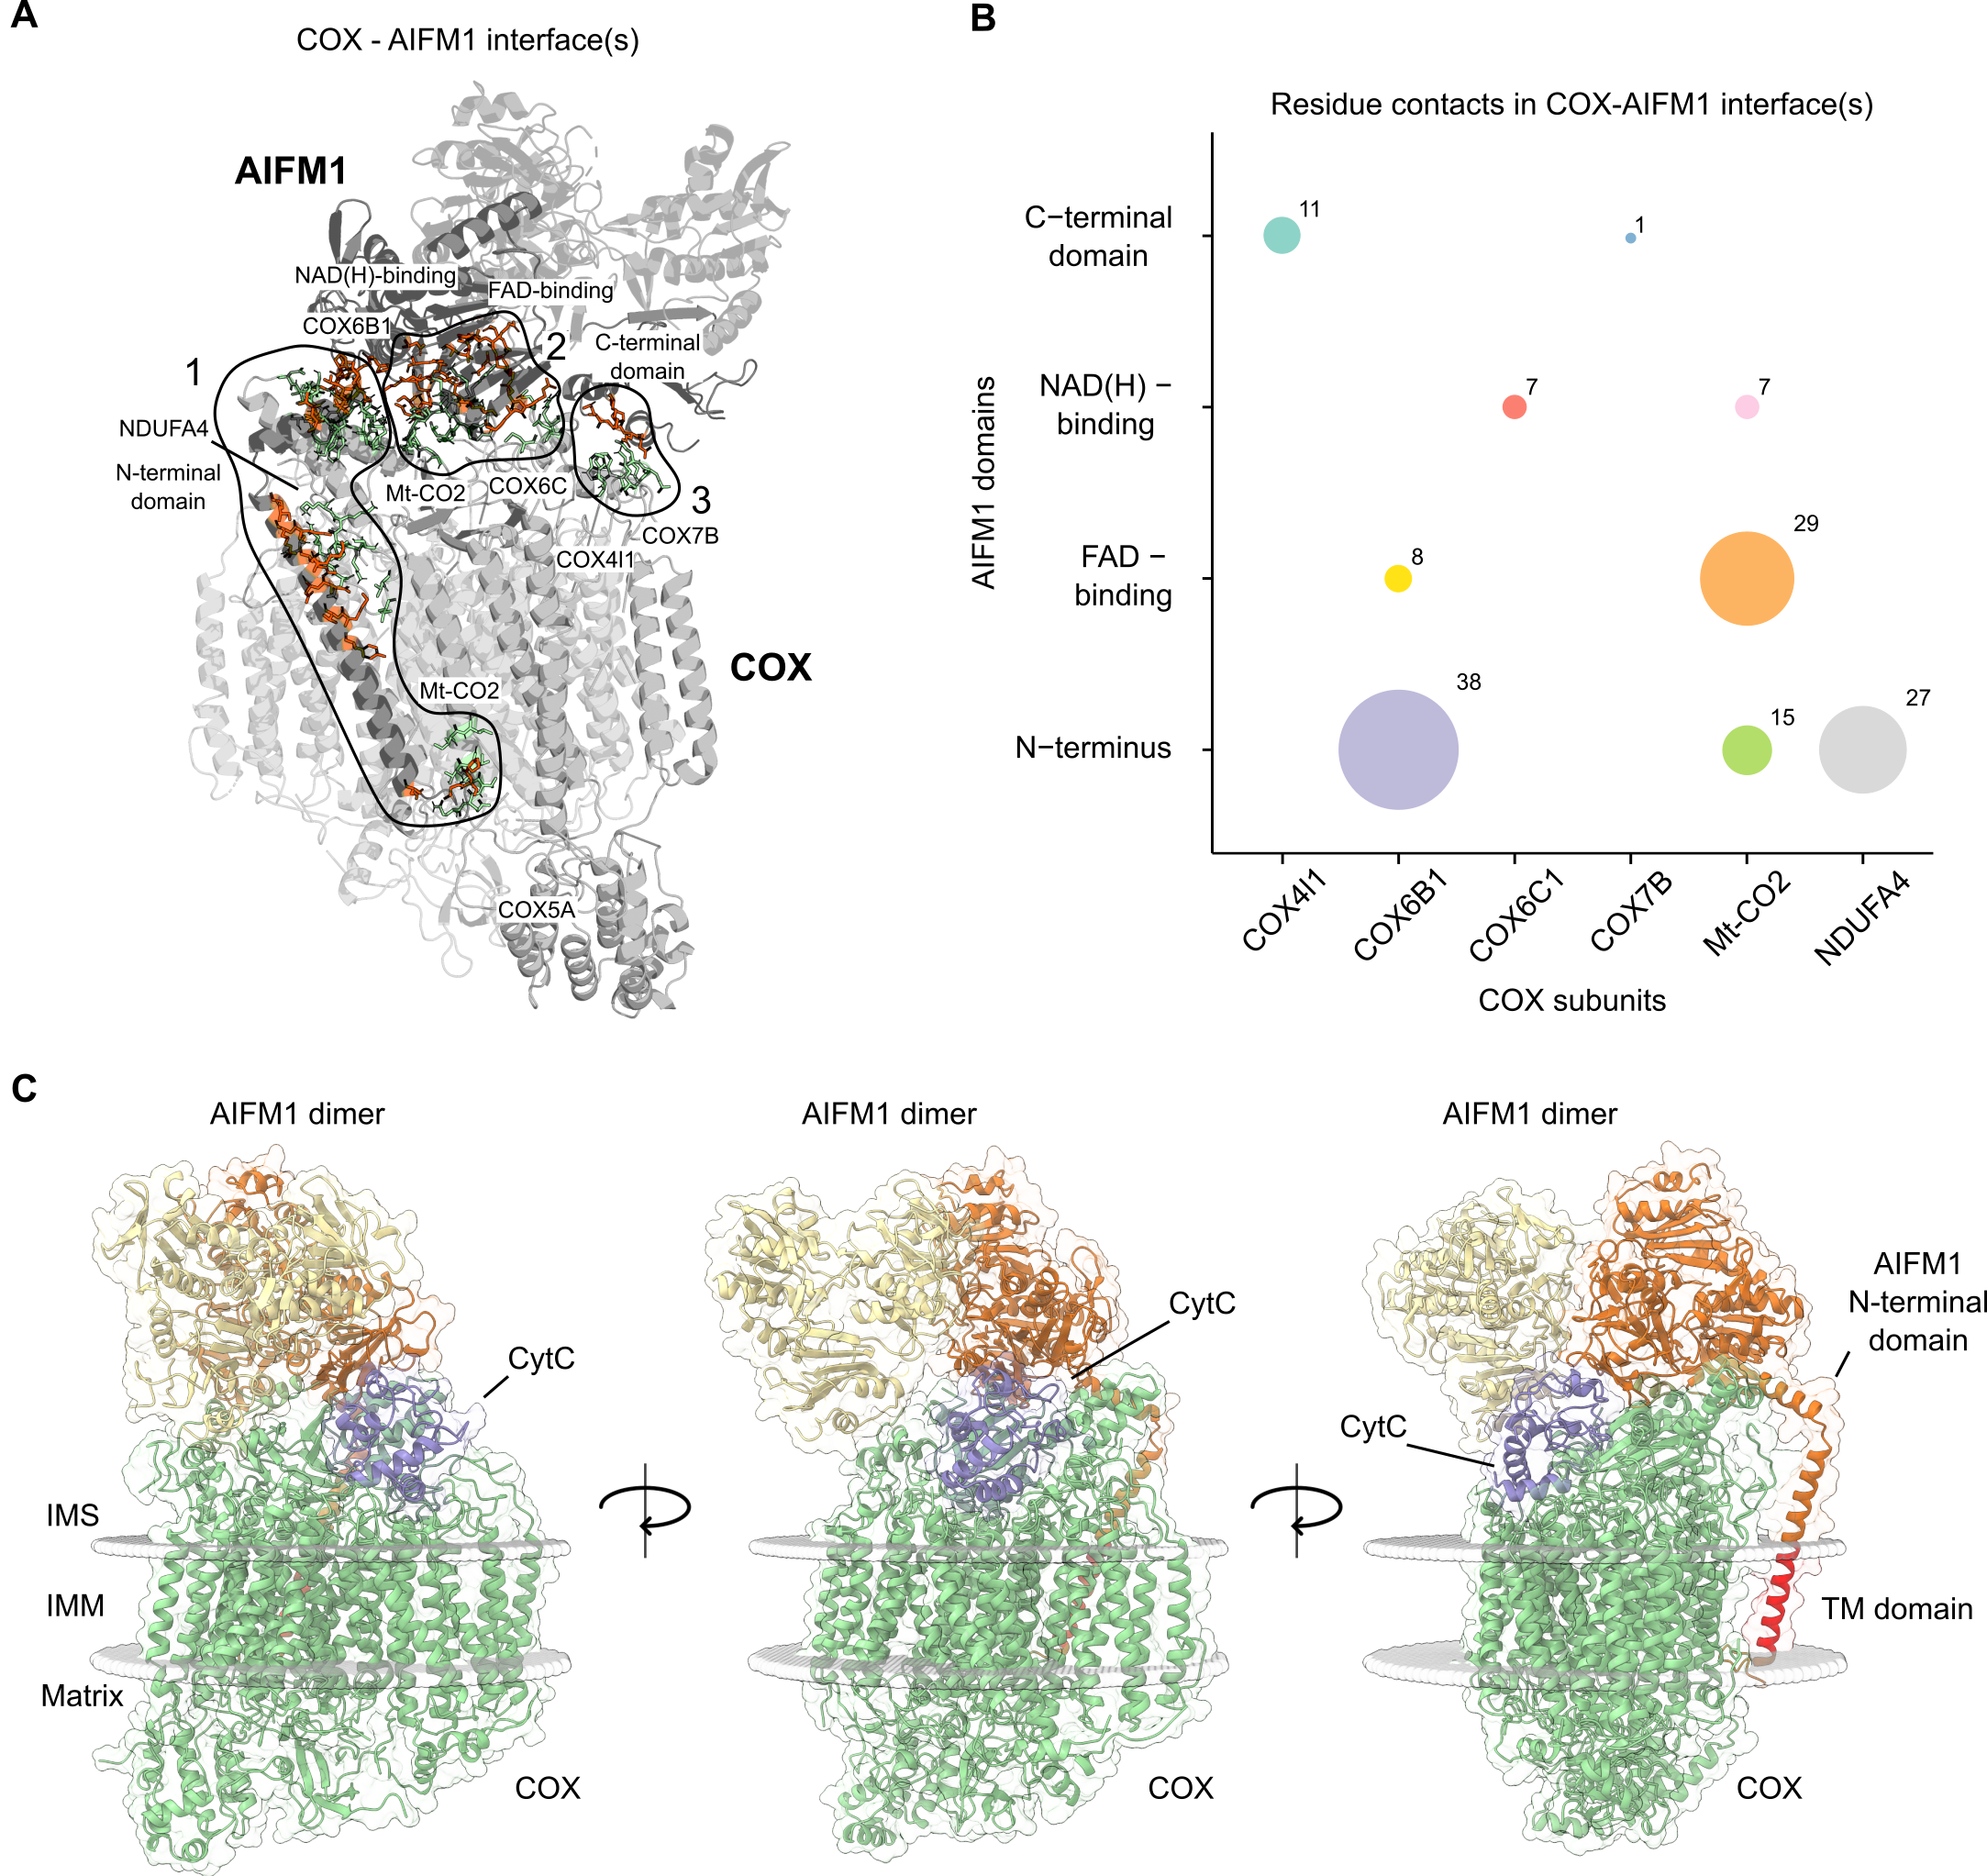
\includegraphics[]{Chapter.3/Figures/Figure4.png}
	\caption{\textbf{Deciphering interaction interfaces in the COX-AIFM1\textsubscript{2} structural model.} \textbf{A.} Three distinct interfaces between COX subunits and respective AIFM1 protomers were found. Subunits (COX) and protein domains (AIFM1) with residues in respective interfaces are colored in gray. Active COX residues are shown as green colored sticks and active AIFM1 residues as orange colored sticks. \textbf{B.} Analysis of the number of residue contacts between respective COX subunits and AIFM1 domains. Colored circles indicate residue contacts between single subunits (COX) and domains (AIFM1) with the size of each circle corresponding to the number of residue-residue interactions. \textbf{C.} COX-AIFM1\textsubscript{2} complex with cytochrome \emph{c} (purple) bound to its COX binding site. The structural model presented here was merged with a previously published model of cytochrome \emph{c} docked to COX from bovine heart \cite{RN54}. COX subunits are colored green, while AIFM1 protomers are colored orange and yellow. The transmembrane (TM) domain of the N-terminal domain of AIFM1 is highlighted in red. Boundaries of the IMM are indicated as gray spheres.}
	\label{fig:ch3_fig4}
\end{figure*}
If COX-AIFM1\textsubscript{2} is not a catalytic complex, it is still tempting to speculate that a ternary interaction of COX, AIFM1\textsubscript{2} and cytochrome \emph{c} could play a role in mitochondrial pro-apoptotic mechanisms. Apart from directly promoting programmed cell death \cite{RN55, RN56, RN5}, AIFM1 could play an indirect role in apoptosis by modulating release of cytochrome \emph{c} \cite{RN1} through its binding to the COX-AIFM1\textsubscript{2} complex. For this, it is important to note that cytochrome \emph{c} makes direct contact to the first AIFM1 protomer in the ternary complex (\textbf{\autoref{fig:ch3_fig4}C}). It is important to note that a structure of bovine COX obtained by X-ray crystallography with its substrate bound \cite{RN57} showed CytC in a position that is different from the one suggested by the model of Sato et al. \cite{RN54} and that would not allow simultaneous binding of AIFM1. However, this apparent discrepancy is not unexpected, since different binding modes of CytC to COX were reported a long time ago based on chemical modification and kinetic studies \cite{RN58} and were confirmed recently by cryoEM analysis \cite{RN59}. Thus, different enzyme-substrate binding modes of CytC including the ones suggested by the docking model and the crystal structure may be physiologically relevant. In any case, the model by Sato et al. \cite{RN54} indicates that it is possible for CytC to bind in a position to COX that allows the formation of a ternary complex with AIFM1. Providing further support for this hypothetical ternary complex, cross-links between AIFM1 and cytochrome \emph{c} were previously reported in intact mouse heart mitochondria \cite{RN16}. However, it is also known that binding of cytochrome \emph{c} to COX is strongly reduced at higher ionic strength \cite{RN60}, which could explain, why we did not observe cross-links between cytochrome \emph{c} and the COX-AIFM1\textsubscript{2} complex. Since the N-terminal pro-peptide with its transmembrane helix provides a significant portion of the AIFM1/COX interface, the complex is expected to destabilize upon cleavage of AIFM1 thereby activating its pro-apoptotic function. In addition to cleaved AIFM1, any previously bound cytochrome \emph{c} would be released concomitantly further promoting apoptosis, potentially providing a synergistic boost to the cell death program already underway.
%
\section{Conclusion}
We show that $\sim$10\% of monomeric COX in bovine heart mitochondria are engaged in a defined complex with dimeric AIFM1. Using structural restraints provided by cross-linking data, available high-resolution structures and structural modeling, we could derive a model of the COX-AIFM1\textsubscript{2}  complex with and without bound cytochrome \emph{c}. Combining chemical cross-linking and complexome profiling provided useful complementary information and represents proof-of-concept for our experimental approach demonstrating that it can be used to define and characterize multiprotein assemblies in detail that may have been overlooked by other means.

While our structural model excludes direct electron transfer between AIFM1 and COX, it provides clues on potential functional implications of the formation of the COX-\textsubscript{2} complex including a possible involvement in promoting apoptosis. The structural insights into this unexpected mitochondrial complex will stimulate and guide further studies on the role of AIFM1 in OXPHOS biogenesis and apoptosis.
%
\section{Materials and Methods}
%
\subsection*{Isolation and purification of bovine heart mitochondria (BHM)}
Mitochondrial membranes from bovine heart were isolated and preserved as described in \cite{RN11}. In order to increase the purity of the preparation and for Tris-buffer removal, frozen crude mitochondria (4 x 15 ml aliquots; 60 mg protein/ml) were thawed on ice, diluted (1:4) with ice-cold SEH buffer (250 mM sucrose, 1 mM EDTA, 20 mM HEPES, pH 7.4 adjusted with NaOH) and centrifuged at 1,000 x g (10 min; 4°C). The supernatants were recovered and centrifuged at 40,000 x g (20 min; 4°C) and each resulting pellet was suspended in 2 ml SEH buffer. Afterwards, mitochondria were loaded onto a two-layer sucrose gradient (1 M sucrose, 20 mM HEPES, pH 7.4 /1.5 M sucrose, 20 mM HEPES, pH 7.4) and centrifuged at 60,000 x g (20 min; 4°C). The pure mitochondrial fractions accumulated at the interphase were carefully recovered and pooled into one tube. After resuspension in 20 ml ice-cold SEH buffer, pure mitochondria were centrifuged at 10,000 x g (20 min; 4°C) and finally suspended in 5 ml ice-cold SEH buffer supplemented with protease inhibitor cocktail (SIGMAFAST™). Protein concentration was determined by the DC protein assay (Bio-Rad) and aliquots of pure mitochondria were shock-frozen in liquid nitrogen and stored at -80°C until use.
%
\subsection*{Cross-linking of BHM sample with DSSO, PhoX and DMTMM}
Purified bovine heart mitochondrial membranes were buffer exchanged into cross-linking buffer (10 mM HEPES pH 7.8, 1 mM EDTA, 1 mM EGTA, 10 mM NaCl, 150 mM KCl, protease inhibitor). After optimization of the cross-link reaction, $\sim$2 mg of BHM were either incubated with DSSO (0.5 mM freshly re-suspended in anhydrous DMSO; Thermo Fisher Scientific), PhoX (1 mM freshly re-suspended in anhydrous DMSO; made in-house) or DMTMM (10 mM freshly re-suspended in cross-linking buffer; Sigma-Aldrich) in 2 ml of cross-linking buffer at room temperature (RT). The cross-link reaction was quenched after 30 min by the addition of 50 mM Tris (1 M Tris buffer, pH 8.5) for additional 30 min at RT.
%
\subsection*{Sample preparation for XL-MS analysis of cross-linked BHM}
Cross-linked mitochondria were solubilized with Digitonin (9 g/g protein) for 30-60 min on ice. Proteins were denatured and purified as described previously \cite{RN61}. Briefly, denatured proteins were re-suspended and digested overnight (ON) at 37°C with Lys-C followed by Trypsin. The final peptide mixtures were desalted with solid-phase extraction C18 columns (Sep-Pak, Waters). Samples cross-linked with DSSO and DMTMM were fractionated with an Agilent 1200 HPLC pump system (Agilent) coupled to an strong cation exchange separation column (Luna SCX 5 $\mu$m - 100 Å particles, 50 $\times$ 2mm, Phenomenex), resulting in 24 fractions . For PhoX cross-linking we used a Fe3+-IMAC column (Propac IMAC-10 4 $\times$ 50 mm column, Thermo Fisher scientific) connected to an Agilent HPLC. Lyophilized peptides were dissolved in buffer A (30\% acetonitrile, 0.07\% trifluoroacetic acid) and the pH was adjusted to a value of 2. PhoX cross-linked peptides were subsequently eluted with a gradient of elution buffer B (0.3\% NH4OH) \cite{RN62}. The collected PhoX-enriched peptides were then dried down and further fractionated into 7 high-pH fractions as previously described \cite{RN63}.
%
\subsection*{XL-MS analysis and data analysis}
The 24 SCX fractions of DSSO were injected in an Agilent 1290 Infinity UHPLC system (Agilent) on a 50-cm analytical column packed with C18 beads (Dr Maisch Reprosil C18, 3 $\mu$m) coupled online to an Orbitrap Fusion Lumos (Thermo Fisher Scientific). We used the following LC-MS/MS parameters: after 5 minutes of loading with 100\% buffer A (water with 0.1\% formic acid), peptides were eluted at 300 nL/min with a 97 minutes gradient from 4\% to 39\% of buffer B (80\% Acetonitrile and 20\% water with 0.1\% formic acid). For MS acquisition we used a MS1 Orbitrap scan at 120,000 resolution from 310 to 1600, AGC target of 5e\textsuperscript{5} ions and maximum injection time of 50 ms. The ions with a charge from +3 to +8 were fragmented with CID (NCE of 30\%) and analyzed with MS2 Orbitrap at 30,000 resolution, AGC target of 5e\textsuperscript{4} ions and maximum injection time of 54 ms for detection of DSSO signature peaks (difference in mass of 37.972 Da). The four ions with this specific difference were analyzed with a MS3 Ion Trap scans (AGC target of 2e\textsuperscript{4} ions, maximum injection time of 150 ms) for sequencing the individual peptides. For the fractions of DMTMM and PhoX, we used an Ultimate3000 (Thermo Fisher Scientific) and 50-cm analytical column packed with C18 beads (Dr Maisch Reprosil C18, 3 $\mu$m) heated at 45°C, connected to Orbitrap Fusion Lumos. For both experiment we used a gradient from 9\% to 40\%, but in case of DMTMM it was 90 minutes long while for PhoX 30 minutes. For both experiments, we used a MS1 Orbitrap scan at 120,000 resolution from 350 to 1400, AGC target of 1e\textsuperscript{6} ions and maximum injection time of 50 ms. The most abundant ions with a charge between +3 and +8 were fragmented in HCD (stepped NCE of 30±3\%) and analyzed with MS2 Orbitrap scan at 30,000 resolution, AGC target of 1e\textsuperscript{5} ions, and maximum injection time of 120 ms. The DSSO fractions were analyzed with Proteome Discoverer software suite version 2.4.1.15 (Thermo Fisher Scientific) with the incorporated XlinkX node for analysis of cross-linked peptides as reported by Klykov et al. \cite{RN64}. Data were searched against a FASTA file containing the $\sim$4200 most abundant proteins, which were previously determined following a classical bottom-up workflow. Were applicable, mitochondrial target peptides were removed from respective protein sequences. For XlinkX search, we selected fully tryptic digestion with three maximum missed cleavages, 10 ppm error for MS1, 20 ppm for MS2 and 0.5 Da for MS3 in Ion Trap. For modifications, we used static Carbamidomethyl (C) and dynamic Oxidation (M). The cross-linked peptides were accepted with a minimum score of 40, minimum score difference of 4 and maximum FDR (controlled at PSM level for cross-linked spectrum matches) rate set to 5\%. Both non-cleavable cross-linkers were analyzed with pLink2 \cite{RN65} and the same FASTA used for DSSO. For PhoX, we manually added the cross-linker to the list (alpha/beta sites “[K”, linker composition C(8)H(3)O(5)P(1) mass of 209.971Da) and for both cross-linkers, the same parameter settings as described for XlinkX was used with following exceptions: no minimum score option and the FDR was calculated separately for intra and inter cross-links. Finally, cross-links were additionally filtered: only cross-links corresponding to protein-protein interactions that were reported for at least two cross-linkers and with at least two CSMs were kept for the final interaction analysis and structural modeling.
%
\subsection*{Complexome profiling analysis}
Aliquots of untreated and PhoX and DMTMM cross-linked mitochondrial membranes (see “Cross-linking of BHM sample with DSSO, PhoX and DMTMM” for details) were thawed on ice, solubilized with digitonin (9 g/g protein) in 50 mM NaCl, 50 mM imidazole-HCl, 2 mM 6-aminohexanoic acid, 1 mM EDTA, pH 7 and kept on ice for 20 min. Samples were further centrifuged at 22,000 $\times$ g (20 min; 4°C) and the supernatants were transferred into clean tubes and supplemented with Coomassie blue loading dye as described in I. Wittig, et al. \cite{RN66}. For blue-native (BN)-PAGE, 100 $\mu$g protein of each sample were loaded onto 4-16\% or 3-10\% polyacrylamide gradient gels and separated as described previously \cite{RN66}. After the electrophoretic run, the gel was fixed ON in 50\% methanol, 10\% acetic acid, 100 mM ammonium acetate followed by staining with 0.025\% Coomassie blue G-250 (Serva G) in 10\% acetic acid for 30 min, de-stained twice in 10\% acetic acid (1 h each) and kept in deionized water ON. The next day, the gel was color-scanned using a flatbed Image Scanner III (GE, USA) to use it as a template for the cutting procedure. Proteins were identified by LC-MS/MS after in-gel tryptic digestion following the protocol described in H. Heide, et al. \cite{RN15} with some modifications. In short, each gel lane was cut into 60 even slices starting at the bottom of the gel. The slices were cubed and transferred into 96-well filter plates (Millipore\textsuperscript{®}, MABVN1250) adapted manually to 96-well plates (MaxiSorpTM Nunc) as waste collectors. Gel pieces were incubated with 50\% methanol, 50 mM ammonium hydrogen carbonate (AHC) under moderate shaking; the solution was refreshed until the blue dye was removed completely. Removal of excess solution was done by centrifugation (1,000 $\times$ g, 15 s). In the next step, gel pieces were reduced with 10 mM dithiothreitol in 50 mM AHC for 1 h. After removing excess solution, 30 mM chloroacetamide in 50 mM AHC was added to each well, incubated in the dark for 45 min and removed. A short incubation step with 50\% methanol, 50 mM AHC was performed for gel pieces dehydration ($\sim$15 min). The latter solution was removed and gel pieces were dried for $\sim$30 min at RT. Later, 20 $\mu$l of 5 ng $\mu$l-1 trypsin (sequencing grade, Promega\textsuperscript{®}) in 50 mM AHC plus 1 mM CaCl2 were added to each well and incubated for 20 min at 4°C. Gel pieces were covered by adding 50 $\mu$l of 50 mM AHC followed by an ON incubation at 37°C for protein digestion. The next day, the peptide-containing supernatants were collected by centri¬fugation (1,000 $\times$ g, 30 s) into clean 96-well PCR plates (Axygen\textsuperscript{®}). The gel pieces were finally incubated with 50 $\mu$l of 30\% acetonitrile (ACN), 3\% formic acid (FA) for $\sim$30 min prior elution of the remain¬ing peptides on the previous eluates by centrifugation. The peptides were dried in a SpeedVac Concentrator Plus (Eppendorf) for 2.5-3 hours, resuspended in 20 $\mu$l of 5\% ACN, 0.5\% FA and stored at -20 °C until MS analysis. After thawing the frozen resuspended peptides and a 30 min gentle shaking, individual samples were loaded and separated by reverse phase liquid chromatography and analyzed by tandem mass spectrometry in a Q-Exactive Orbitrap Mass Spectrometer equipped with a nano-flow ultra-HPLC system (Easy nLC1000, Thermo Fisher Scientific). In brief, peptides were separated using 100 $\mu$m ID $\times$ 15 cm length PicoTipTM EMITTER columns (New Objective) filled with ReproSil-Pur C18-AQ reverse-phase beads (3 $\mu$m, 120Å) (Dr. Maisch GmbH, Germany) using linear gradients of 5\%-35\% ACN, 0.1\% FA (30 min) at a flow rate of 300 nl min-1, followed by 35\%-80\% ACN, 0.1\% FA (5 min) at 600 nl min-1 and a final column wash with 80\% ACN (5 min) at 600 nl min-1. All settings for the mass spectrometer operation were the same as detailed in \cite{RN34}.
MS raw data files from all individual slices were analyzed using MaxQuant (v1.5.0.25) against the \emph{Bos taurus} proteome entries retrieved from Uniprot. The following settings were applied: Trypsin, as the protease, N-terminal acetylation and methionine oxidation as variable modifications; cysteine carbamidomethylation as fixed modification; two trypsin missed cleavages; matching between runs, 2 min matching time window; six residues as minimal peptide length; common contaminants included; I = L and the rest of parameters were kept as default. Individual protein abundances were determined by label-free quantification using the obtained intensity-based absolute quantification (iBAQ) values, which were corrected for protein loading and MS sensitivity variations using the sum of total iBAQ values from each sample. For each protein group entry, migration profiles were generated and normalized to the maximal abundance through all fractions. The migration patterns of the identified proteins were hierarchically clustered by an average linkage algorithm with centered Pearson correlation distance measures using Cluster 3.0 \cite{RN67}. The resulting complexome profiles consisting of a list of proteins arranged according to the similarity of their migration patterns in BN-PAGE were visualized as heatmaps representing the normalized abundance in each gel slice by a three-color gradient (black/yellow/red) and processed in Microsoft Excel for analysis. The mass calibration for the BN gel was performed using the apparent molecular masses of either membrane or soluble bovine heart mitochondrial proteins. For membrane proteins: VDAC1 (30 kDa), complex II (123 kDa), complex IV (215 kDa), complex III (dimer, 485 kDa), complex V (700 kDa), complex I (1000 kDa), respiratory supercomplexes, I-IV (1215 kDa), I-III2 (S0, 1485 kDa), I-III2-IV (S1, 1700 kDa), I-III2-IV2 (S2, 1915 kDa) and complex V tetramer (2400 kDa). For soluble proteins: ATP synthase subunit beta (51 kDa), citrate synthase (dimer, 98 kDa), ETFA/B (dimer, 122 kDa), enoyl-CoA hydratase (hexamer, 169 kDa), fumarase (tetramer, 200 kDa), Heat shock protein 60 (heptamer, 406 kDa), PCCA/B (hexamer 762 kDa) and oxoglutarate dehydrogenase complex ($\sim$2500 kDa).
%
\subsection*{Generation of structural models for COX and AIFM1}
Firstly, as no structure of bovine (dimeric) AIFM1 is currently available, a homology model was generated and structurally aligned based on the human dimeric AIFM1 structure (PDB: 4BUR) using Robetta. The final dimeric model of AIFM1 lacks the N-terminal region, containing residues 128-516 and 551-611 for both molecules. The N-terminal region of AIFM1 (res 55-124) was generated using trRosetta \cite{RN39}. Further, a monomeric COX structure was generated from the recently published bovine COX dimer (PDB: 1V54). The structure was modified by adding the missing NDUFA4 subunit, which was modelled and structurally aligned based on the human homolog (PDB: 5Z62 chain N) using Robetta. Likewise, missing residues (without transit peptides) for COX6B1 and COX5A subunits were modelled and added to the COX and added to the final COX structure used for docking.
%
\subsection*{Cross-linking driven docking and analysis of a COX-AIFM1\textsubscript{2} complex}
To generate a COX-AIFM1 structure, modified structures for COX, AIFM1 and the N-terminal domain of AIFM1 were used. Firstly, interaction interfaces and cross-links supporting a distinct complex formation were identified using DisVis \cite{RN44}. Active residues involved in an interface were computed additionally based on solvent accessible residue information. Solvent accessible residues (absolute and relative solvent accessibility $\geq$ 40\%) were identified using the standalone program Naccess (© S. Hubbard and J. Thornton 1992-6). Structural docking with respective structures was done in Haddock \cite{RN68, RN45} using predicted active residues and cross-links as additional restraints. Different distance allowances between C$\alpha$-C$\alpha$ atoms were used based on the observed cross-link: DSSO = 35 Å, PhoX = 30 Å and DMTMM = 25 Å. Docking of COX, the AIFM1 dimer and one N-terminal domain of AIFM1was performed separately, to ensure correct positioning of the N-terminal domain of AIFM1 with respect to COX and the respective AIFM1 protomer. The missing residues of the flexible linker between the AIFM1 protomer and the N-terminal domain were built afterwards to complete the structure and to further verify the positioning of the N-terminal domain. Missing residues for cross-linked subunits of COX involved in the COX-AIFM1 interaction were modelled before the docking procedure. The finally chosen model was the best scoring model within the best scoring cluster which also supported the cross-linking restraints best. Subsequently, the “Model Loops” of Chimera (Version 1.14rc) \cite{RN47, RN46} was applied to model missing residues (125-127) and structurally connecting the N-terminal domain of AIFM1 (res 55-124) and respective AIFM1 protomer (28-516; 551-613). Interface residues of the resulting COX-AIFM1\textsubscript{2}  complex were identified using the Prodigy web service \cite{RN69}. To determine whether cytochrome \emph{c} can still potentially bind to its COX binding site in the COX-AIFM1\textsubscript{2}  complex, this protein was structurally aligned based on a previously solved structure of cytochrome \emph{c} docked to COX from bovine heart \cite{RN54}. Presented membrane boundaries for all presented structures were added using either the OPM \cite{RN70} webserver or MemprotPD \cite{RN71}.
%
\subsection*{Data availability}
All cross linking mass spectrometry related data, the structural docking (Haddock results), and the presented COX-AIFM1/ COX-AIFM1-CytC structural model described in this work have been deposited to the ProteomeXchange partner (PRIDE) database and assigned the identifier PXD025102 \cite{RN72}. Complexome profiling datasets have been deposited in the CEDAR database and assigned the identifier CRX33 \cite{RN73}. The structural model of COX-AIFM1\textsubscript{2} complex is provided in the PDB-DEV repository (PDBDEV\_00000092). Supplementary Datasets are available online with the original manuscript (Supporting Information).
%
\subsection*{Acknowledgments}
All authors acknowledge support from the Netherlands Organization for Scientific Research (NWO) funding the Netherlands Proteomics Centre through the X-omics Road Map program (Project 184.034.019) and the TOP project 714.017.004, the Netherlands Organization for Health Research and Development (ZonMW TOP 91217009), the EU Horizon 2020 program Epic-XS (Project 823839), and the German Research Foundation (DFG) through the Collaborative Research Center 1218 (Project 269925409).
%
\subsection*{Author contributions}
JFH, UB, SA and AJRH designed the study. JFH and RCZ performed XL-MS experiments. JFH performed XL-MS analysis and structural modeling. ACO performed the complexome profiling experiments. ACO, SA and UB analyzed the complexome profiling datasets. ACO and SA provided the bovine mitochondrial samples. JFH, SA and AJRH wrote the original draft, with all authors carefully revising and editing the manuscript before submission. UB, SA and AJRH acquired funding and resources. AJRH supervised the project.
%
\subsection*{Conflict of interest}
The authors do not declare any conflict of interest.
%
%%Appendix
\clearpage
\begin{subappendices}
	\counterwithin{figure}{section}
	\section{Supplementary Material}
	\begin{figure*}[hb!]
		\center
		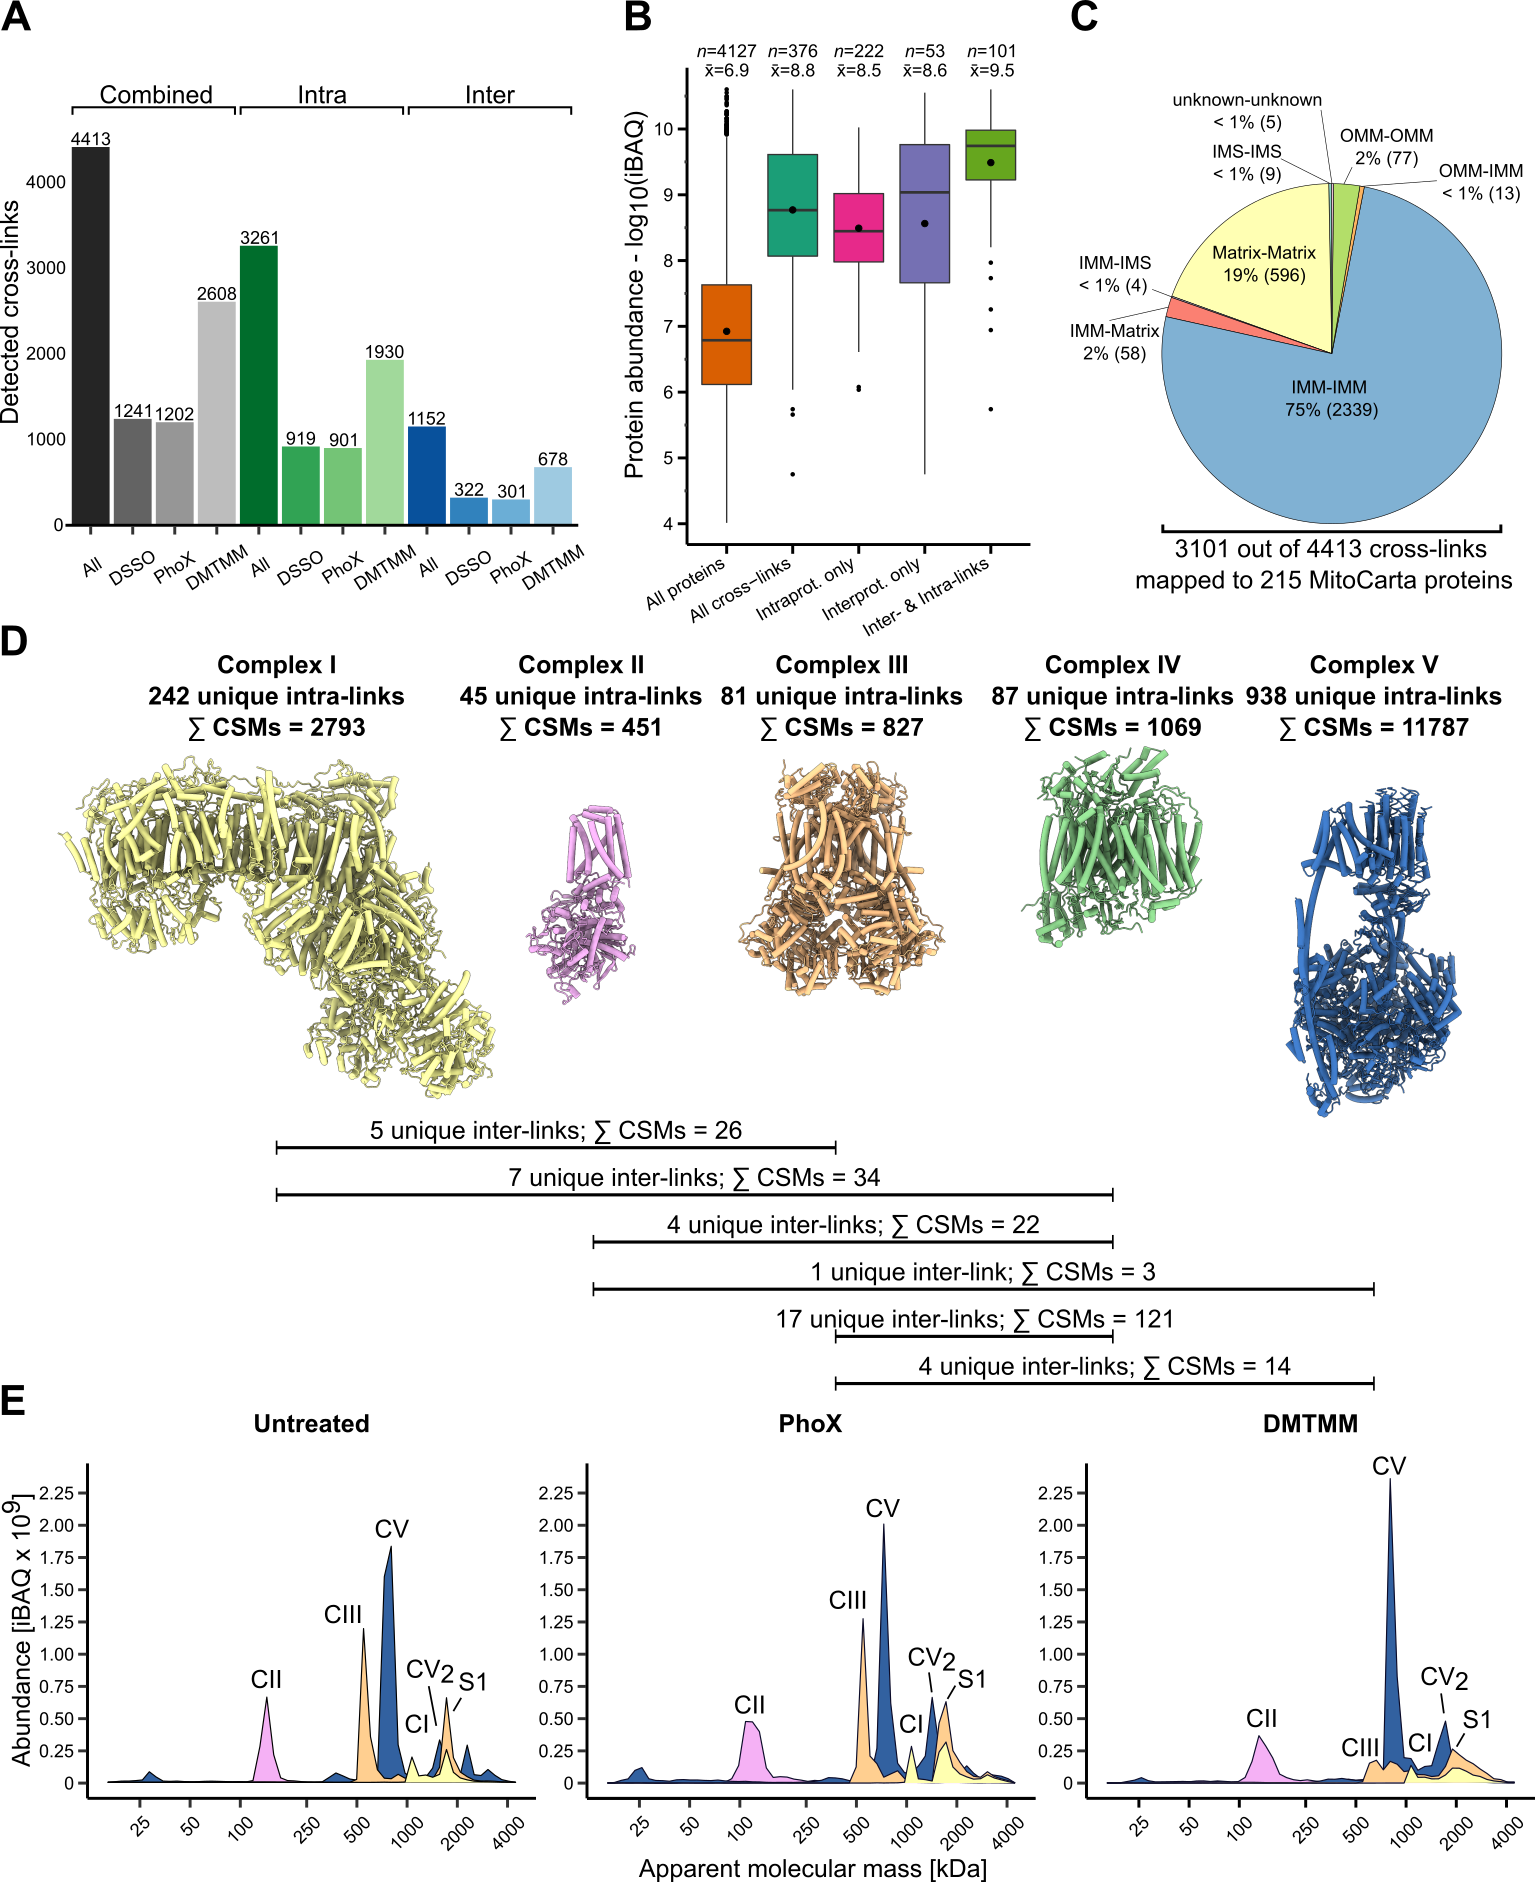
\includegraphics[]{Chapter.3/Figures/SI_Figure1.png}
		\caption{Figure Legend on next page}
		\label{fig:ch3_app_fig1}
	\end{figure*}
	\addtocounter{figure}{-1}
	\begin{figure*}[ht!]
		\caption{\textbf{Overview of cross-linking and complexome profiling of bovine heart mitochondria (BHM).} BHM were cross-linked in parallel with three different cross-linkers (DSSO, PhoX and DMTMM) and subjected to XL-MS analysis or complexome profiling. \textbf{A.} Overview of the number of unique cross-links, identified for each of the cross-linkers used (DSSO, PhoX, DMTMM) and in combination (all). \textbf{B.} Observed cross-linked proteins are generally more abundant. Boxplot showing protein abundances for all identified proteins, all cross-linked proteins and proteins that have either only inter-, intra- or both (inter and intra) links. The number of proteins and the median iBAQ is indicated on top of each box. \textbf{C} Pie chart showing the sub-mitochondrial localization of the cross-linked proteins identified based on their MitoCarta 3.0 annotation. \textbf{D} Numbers of obtained cross-links for OXPHOS complexes I-V. Complexes are heavily cross-linked ($\sim$35\% of all detected cross-links). Cross-links are observed within subunits of the same complex (intra cross-links) but also between subunits of different OXPHOS complexes (inter cross-links). For structural representation, deposited structural models were chosen (PDB: 5LNK, 1ZOY, 1NTM, 1V54, 5ARA). \textbf{E} Averaged migration profiles of the OXPHOS complexes CI, CII, CIII and CV without cross-linker treatment and after treatment with either the PhoX or DMTMM cross-linker using a 4-16\% gradient BN gel. The profiles were obtained by plotting the relative abundance of the averaged subunits of each complex against the respective molecular mass. Peaks are annotated based on the molecular masses of CI, CII, CIII, CV and the supercomplex S1 (CI-CIII\textsubscript{2}-CIV). Upon addition of cross-linker, the OXPHOS complexes largely maintain their overall migration profile, and thus structural integrity.}
	\end{figure*}
	\begin{figure*}[htb]
		\center
		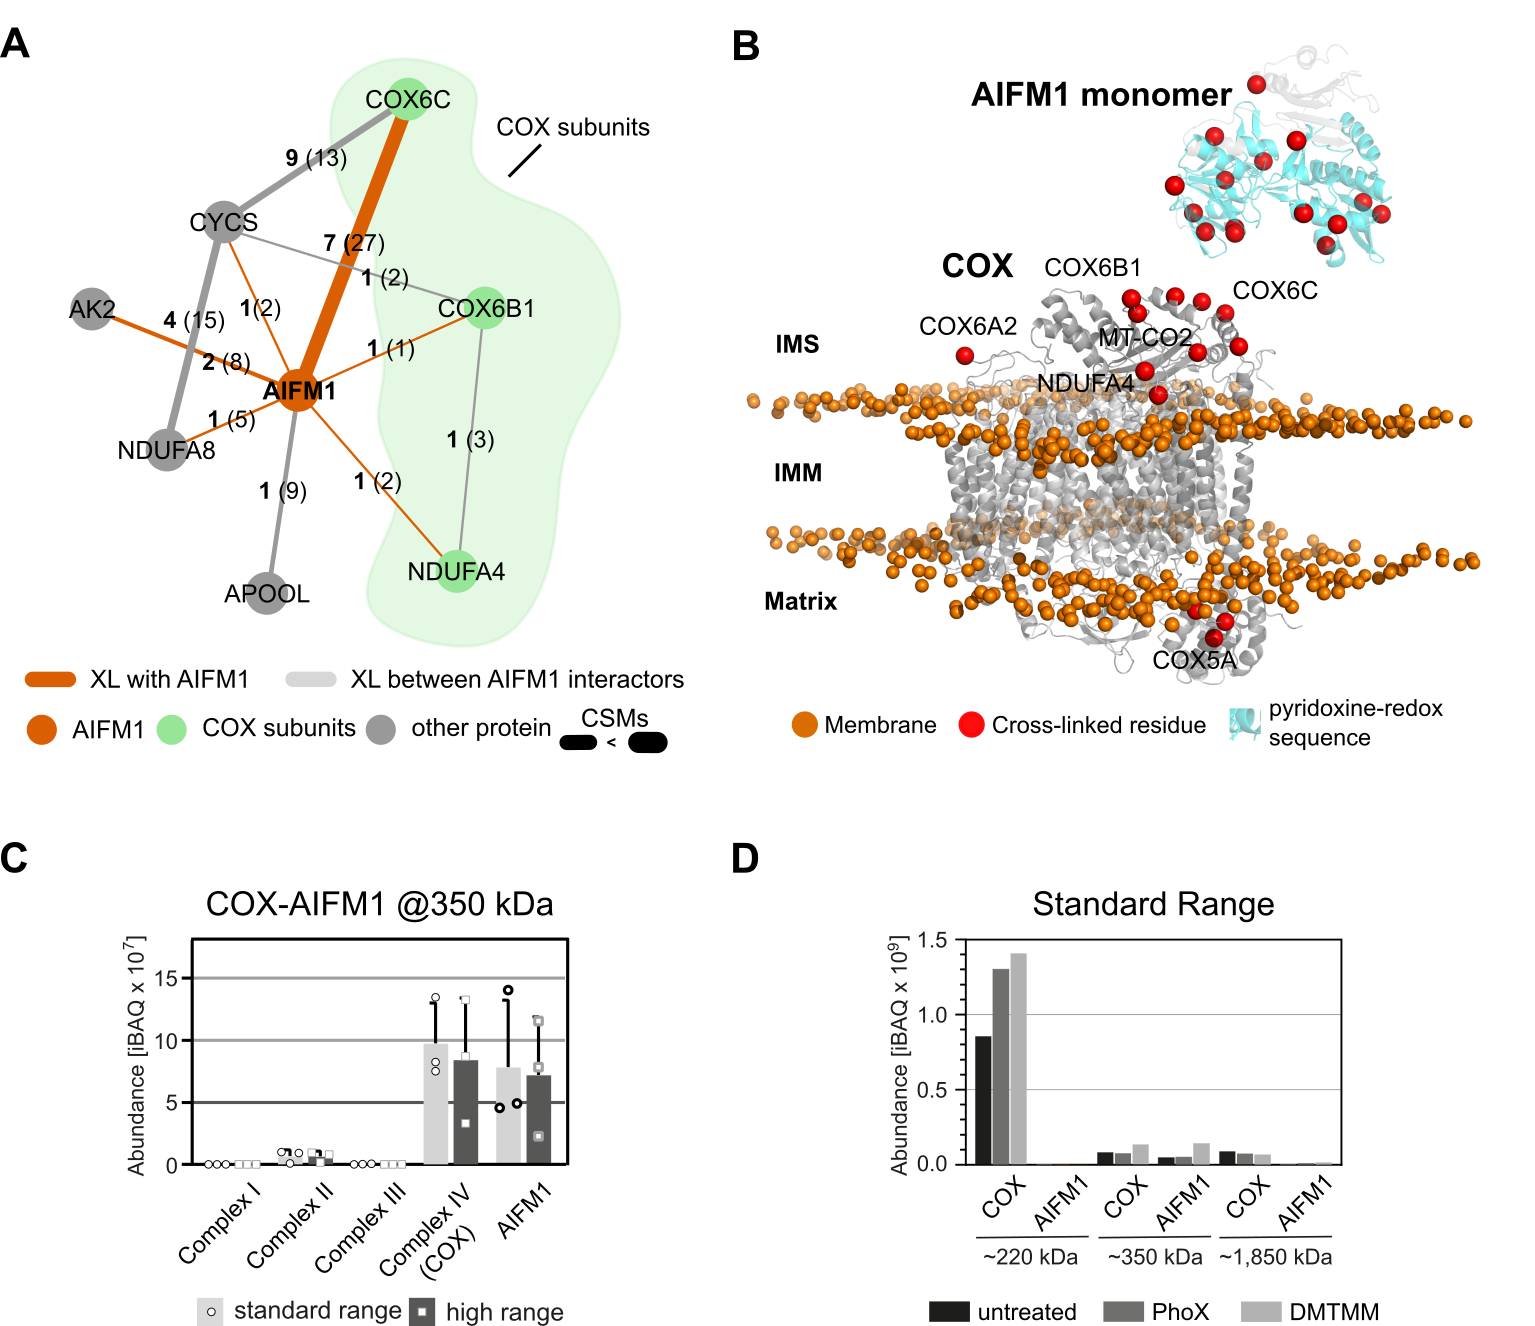
\includegraphics[]{Chapter.3/Figures/SI_Figure2.png}
		\caption{\textbf{COX-AIFM1 interactions.} \textbf{A.} The AIFM1 interactome as observed by XL-MS in intact mouse heart mitochondria adapted from \cite{RN16}. Bold numbers indicate the observed cross-links for each interaction and thickness of lines indicates the cumulative evidence (CSMs) for each interaction (number in brackets). CSMs were summed from triplicates. \textbf{B.} Visualization of cross-linked residues (red spheres) of COX (gray) and truncated AIFM1 monomer (gray with residues of the Pyr-redox sequence being cyan) in our data on BHM. Orange spheres indicate the phosphate groups of a simulated lipid bilayer (IMM) which was structurally aligned based on the simulation for bovine monomeric COX (PDB: 6JY3) obtained from the MemProtMD server. \textbf{C.} Comparison of the amounts of respiratory chain complexes I to IV and AIFM1 at $\sim$350 kDa representative of the COX-AIFM1\textsubscript{2} complex. Complexome profiling was performed using a standard range BN-gel (4-16\%) and a high range BN-gel (3-10\%). The average of individual values ± SD from all three conditions (untreated, PhoX and DMTMM cross-linked) is shown. \textbf{D.} Comparison of COX and AIFM1 abundances at $\sim$220 kDa, $\sim$350 kDa and $\sim$1,850 kDa in complexome profiles using a standard BN-gel (4-16\%) of BHM as prepared (untreated) and after cross-linking with PhoX and DMTMM. In \textbf{C.} and \textbf{D.}, iBAQ values of AIFM1 are divided by two to account for the dimer and the average of subunits of the respective complexes at the indicated approximate apparent masses in the migration profiles were taken as a measure for their abundance.}
		\label{fig:ch3_app_fig2}
	\end{figure*}
	\begin{figure*}[htb]
		\center
		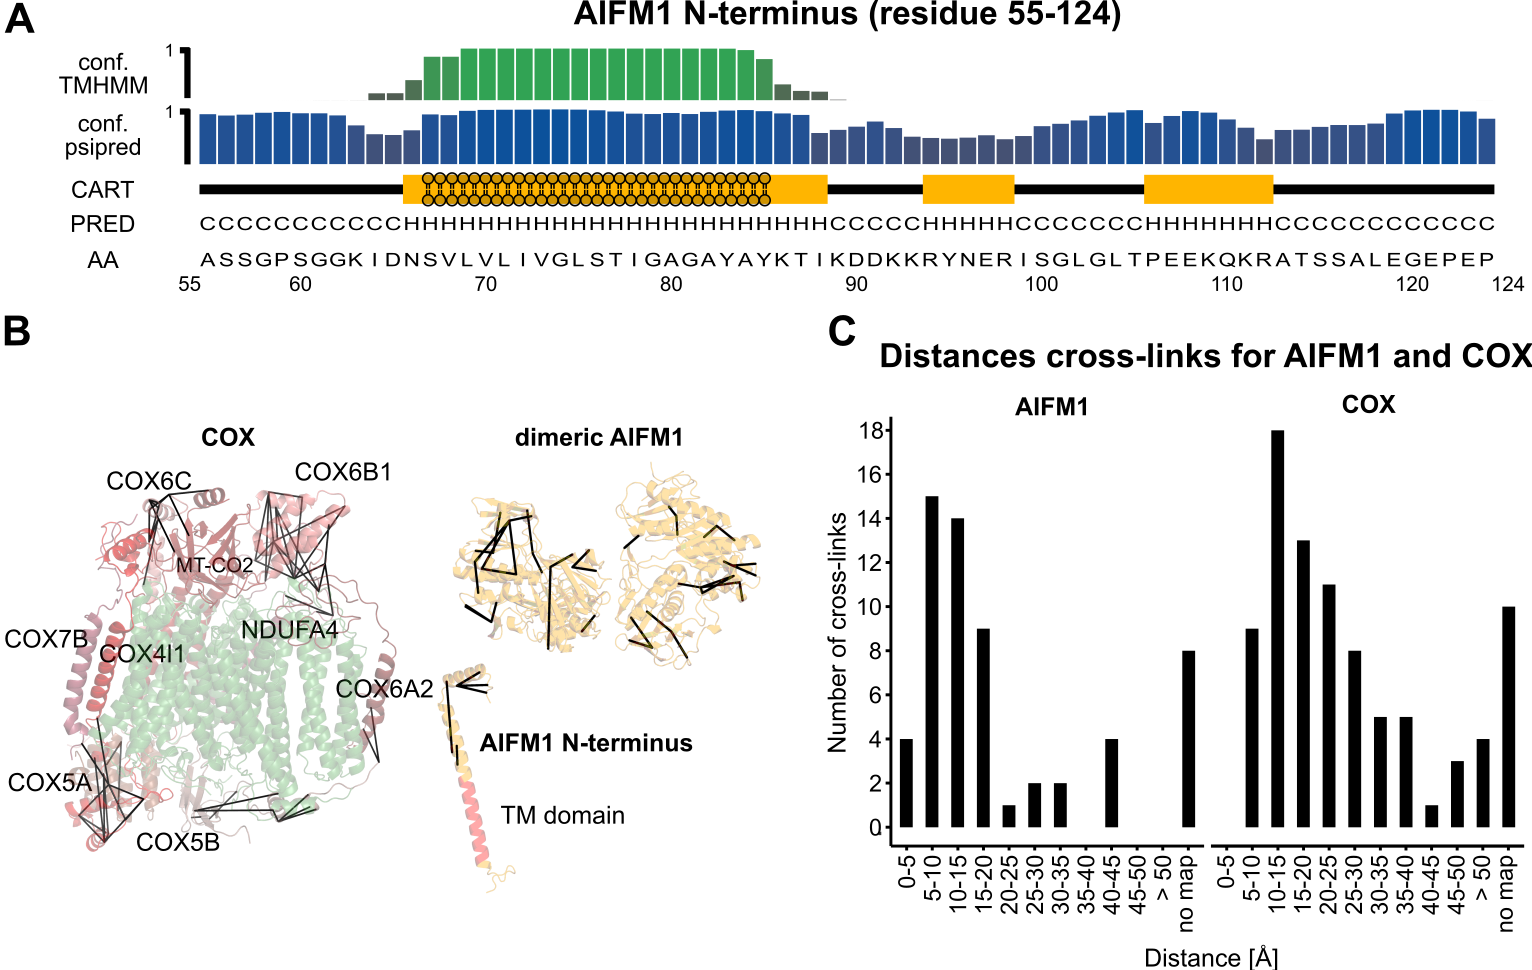
\includegraphics[]{Chapter.3/Figures/SI_Figure3.png}
		\caption{\textbf{Structural properties of the N-terminal region of AIFM1 and cross-link distances in the COX and AIFM1 structures used for docking.} \textbf{A.} Secondary structure prediction of the N-terminal region of AIFM1 (res 55-124; sequence indicated under AA). The upper bar plot shows the confidence of residues being transmembrane residues (Score = 1) or not within a membrane (Score < 0.6). The second bar plot shows the confidence of the secondary structure prediction (1 = highest, 0 = lowest) for each residue which is indicated under PRED as letter code (C = coil, H = helix) und visualized as cartoon under CART. \textbf{B.} Detected cross-links (intra and inter domain) mapped onto the structural models of COX, AIFM1 dimer as well as the de-novo modelled N-terminal domain of AIFM1. The COX structure (green, with cross-linked subunits colored in different shades of red as indicated) was based on a previously resolved structure (PDB: 1V54) supplemented with NDUFA4 (structurally aligned based on PDB: 5Z62). Dimeric AIFM1 (orange) was modelled based on the previously resolved human homologue (PDB: 4BUR, res 128-516, 551-613). The N-terminal domain of AIFM1 (orange) (res 55-124) was generated using trRosetta. The predicted transmembrane (TM) domain is highlighted in red. \textbf{C.} Distance histogram of mapped cross-links (combination of DSSO, PhoX and DMTMM) for COX and AIFM1. AIFM1 includes distances for cross-links mapped on the AIFM1 dimer and the N-terminal region of AIFM1. For both structures, a number of cross-links are obtained within or attaching to missing regions of AIFM1 (N-terminus (55-127) and residue 517-550) and COX (N-terminus COX4l1).}
		\label{fig:ch3_app_fig3}
	\end{figure*}
	\begin{figure*}[htb]
		\center
		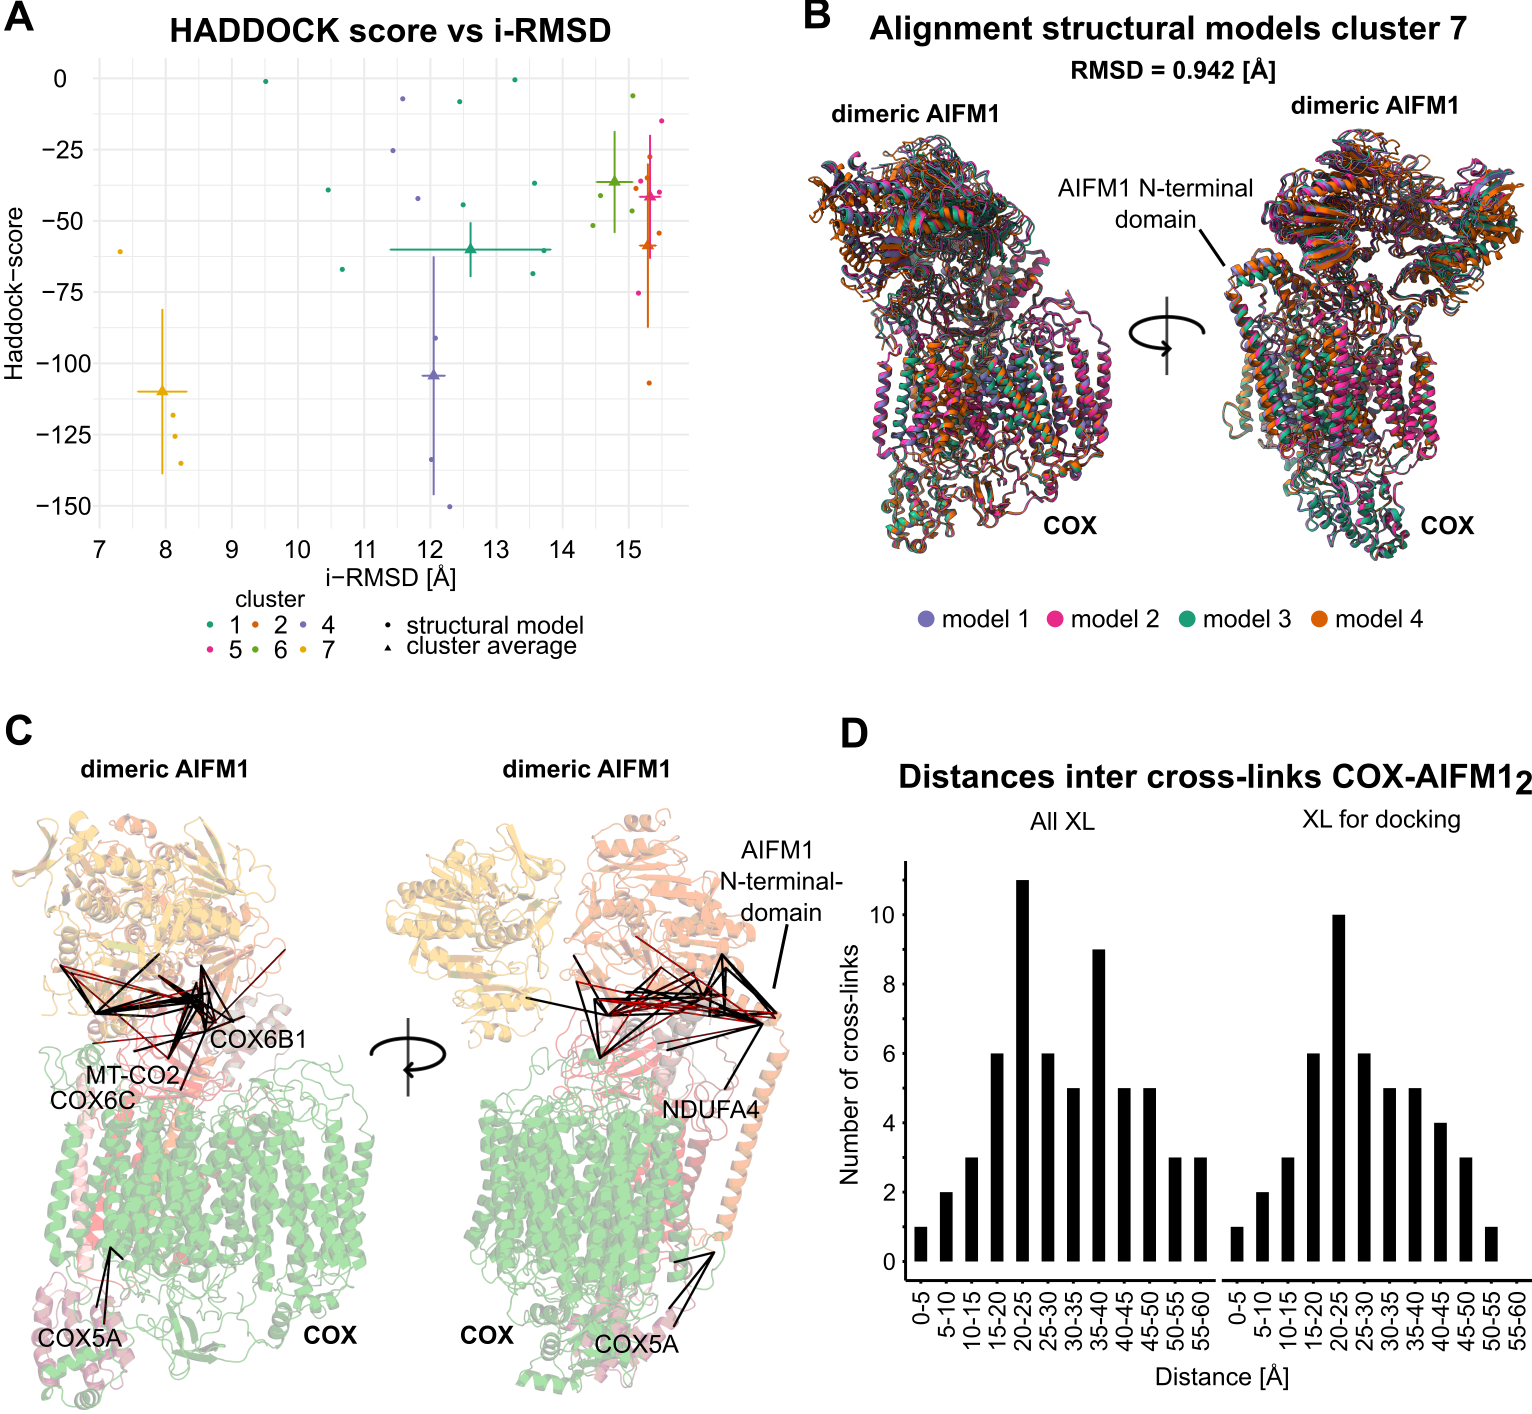
\includegraphics[]{Chapter.3/Figures/SI_Figure4.png}
		\caption{\textbf{Haddock cluster validation and inter cross-link distances in the COX-AIFM1\textsubscript{2} model.} \textbf{A.} Plot of HADDOCK score of the chosen clusters (note: cluster 3 was disregarded due to a positive Haddock score) as a function of their RMSD from the lowest energy structure. Circles represent individual structures of each cluster and triangles correspond to the cluster averages with standard deviation indicated by bars. \textbf{B.} Structural alignment of individual structures of cluster 7. A low average RMSD (0.942 Å) indicates high cluster precision. Different models are colored as indicated. \textbf{C.} Visualization of cross-links between COX and AIFM1 which were used for structural docking of the COX-AIFM1\textsubscript{2} complex. COX subunits are colored green, while AIFM1 protomers are colored orange. Cross-links with a C$\alpha$-C$\alpha$ distance $\leq$ 35 Å are colored in black, while cross-links with a mapped C$\alpha$-C$\alpha$ distance $\geq$ 35 Å are colored in red. Cross-linked subunits of COX are colored in different shades of red as indicated. \textbf{D.} Cross-links (combination of DSSO, PhoX and DMTMM) used for structural docking and all observed cross-links for COX-AIFM1\textsubscript{2} interaction were mapped onto the best model of the complex. For AIFM1, all obtained cross-links can be mapped onto the final structure of AIFM1, containing two AIFM1 protomers (res 128-516, 551-613) and one N-terminal region of one protomer (res 55-124).}
		\label{fig:ch3_app_fig4}
	\end{figure*}
	\begin{figure*}[htb]
		\center
		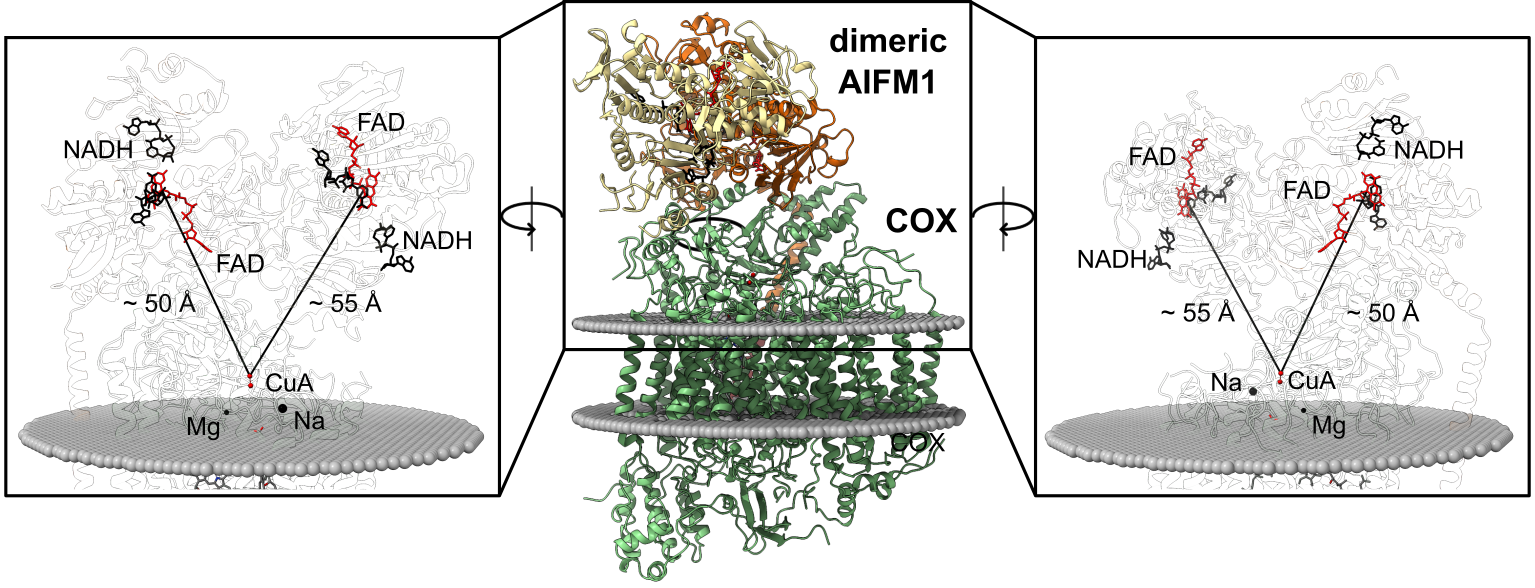
\includegraphics[]{Chapter.3/Figures/SI_Figure5.png}
		\caption{\textbf{Mapping the distance from the isoalloxazine moiety of FAD in AIFM1 to the CuA center of COX.} Cofactors were structurally aligned based on structures of AIFM1 (PDB: 4BUR) and COX (PDB: 1V54). AIFM1 protomers are orange and COX subunits are green (middle); red sticks represent FAD, black sticks represent NADH, CuA, and CuB are red (left and right). Boundaries of the IMM are indicated as gray spheres.}
		\label{fig:ch3_app_fig5}
	\end{figure*}
\end{subappendices}
\clearpage
\section*{References}
\bibliographystyle{Style_settings/bibstyle_pnas}
\bibliography{Chapter.3/chapter3_bib}
\picturechapter{In-cell structures of conserved supramolecular protein arrays at the mitochondria-cytoskeleton interface in mammalian sperm}{Chapter_covers/chapter_cover_4.pdf} \label{ch-4}
\vspace*{0.25cm}

\footnotesize Miguel Ricardo Leung, Riccardo Zenezini-Chiozzi, Marc C. Roelofs, Johannes F. Hevler, Ravi Teja Ravi, Paula Maitan, Min Zhang, Heiko Henning, Elizabeth G. Bromfield, Stuart C. Howes, Bart M. Gadella, Albert J.R. Heck, and Tzviya Zeev-Ben-Mordehai
%
\begin{center}
	\vspace{3cm}
	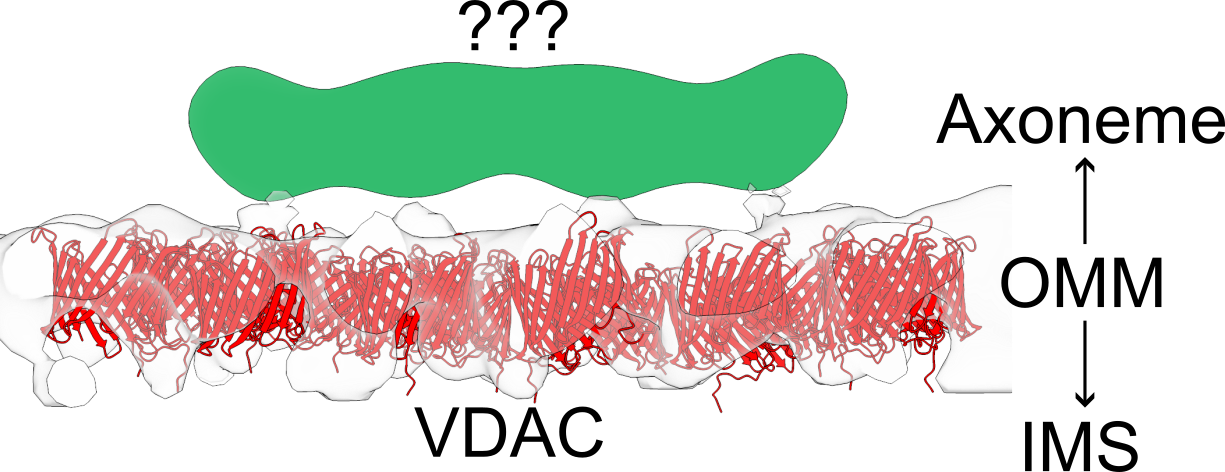
\includegraphics[]{Chapter.4/Figures/Chapter_cover.png}
	\vspace{0.25cm}
\end{center}
%
\begin{flushleft}
	\vspace*{\fill}
	\rule{\textwidth}{1pt}\\[0cm]
	\textbf{This chapter is based on work in the following publication:}\\
	\footnotesize
	\textbf{\emph{PNAS}} (2021), 118:e2110996118, doi:10.1073/pnas.2110996118\\
\end{flushleft}
%%Additional footnote to potentially add for clarification
%{\footnotesize The manuscript resulted from a collaboration which was led by Miguel Ricardo Leung and Tzviya Zeev-Ben-Mordehai. We contributed all proteomics and cross-linking mass spectrometry experiments and respective data analysis.}
\begin{abstract102}
	Mitochondria-cytoskeleton interactions modulate cellular physiology by regulating mitochondrial transport, positioning, and immobilization. However, there is very little structural information defining mitochondria-cytoskeleton interfaces in any cell type. Here, we use cryo-focused ion beam milling-enabled cryo-electron tomography to image mammalian sperm, where mitochondria wrap around the flagellar  cytoskeleton. We find that mitochondria are tethered to their neighbors through intermitochondrial linkers and are anchored to the cytoskeleton through ordered arrays on the outer mitochondrial membrane. We use subtomogram averaging to resolve in-cell structures of these arrays from three mammalian species, revealing they are conserved across species despite variations in mitochondrial dimensions and cristae organization. We find that the arrays consist of boat-shaped particles anchored on a network of membrane pores whose arrangement and dimensions are consistent with voltage dependent anion channels. Proteomics and in-cell cross-linking mass spectrometry suggest that the conserved arrays are composed of glycerol kinase-like proteins. Ordered supramolecular assemblies may serve to stabilize similar contact sites in other cell types where mitochondria need to be immobilized in specific subcellular environments, such as in muscles and neurons.
\end{abstract102}
%%Main Text
\section{Introduction}
\lettrine[lraise=0.1, nindent=0em, slope=-.5em]{I}{n} many cell types, mitochondria collectively form a dynamic network whose members divide, fuse, and communicate with one another \cite{Glancy2015, Viana2020, Vincent2017}. Through interactions with the cytoskeleton, mitochondria are transported - sometimes across large distances - and positioned in response to dynamic stimuli \cite{Fenton2021, Moore2018}. Interactions with the cytoskeleton can also restrain mitochondria to specific subcellular locations. In neurons, axonal mitochondria can be immobilized by interactions with the microtubule or actin cytoskeletons \cite{Chen2013, Gutnick2019, Kang2008}. In cardiac and skeletal muscle, mitochondrial distribution is regulated by interactions with myofibrils and  intermediate filaments \cite{Milner2000, Stone2007}. However, despite the prevalence of intermitochondria and mitochondria-cytoskeleton interactions and their integral roles in cellular function, there is very little information on the molecular architectures of these interaction sites in any cell type.

One of the most striking mitochondrial configurations occurs in amniote sperm, where mitochondria are arranged in a spiral around the axoneme, defining a region called the midpiece \cite{Fawcett1970, Fawcett1975}. Mitochondria are among the few organelles retained in sperm throughout their maturation, during which they otherwise lose most of their cytoplasm and organelles \emph{en route} to becoming highly streamlined cells specialized for finding and fusing with the egg. The extensive mitochondrial sheath in amniote sperm may be an adaptation needed to power the large, long flagellum in these lineages. Variations in midpiece morphometry affect sperm motility and competitiveness \cite{Firman2010, Fisher2016}, and different species rely on energy from mitochondrial respiration to different extents \cite{Tourmente2015, Marin2003}, warranting comparative studies of mitochondrial structure across species.

The core of the midpiece is the flagellar  cytoskeleton, composed of the microtubule-based axoneme and accessory elements called outer dense fibers (ODFs). A poorly-characterized network of cytoskeletal filaments called the submitochondrial reticulum lies between the ODFs and the mitochondria. The submitochondrial reticulum co-purifies with the outer mitochondrial membrane (OMM), suggesting that they are intimately associated \cite{Olson1986, Olson1990}. Mitochondria wrap around the cytoskeleton and are in turn ensheathed by the plasma membrane. As a consequence of this arrangement, each mitochondrion has three distinct surfaces \cite{Olson1992} - one facing the axoneme, one facing the plasma membrane, and one facing neighboring mitochondria. Thin-section electron microscopy (EM) \cite{Olson1992} and freeze-fracture EM \cite{Friend1981, Woolley2005} revealed that each surface is characterized by a unique membrane protein profile. In particular, these studies uncovered an ordered array of particles on the axoneme-facing surface of sperm mitochondria. Notwithstanding the insight gained from these methods, such techniques require harsh sample preparation steps that can distort fine cellular structure and limit achievable resolution \cite{Al-Amoudi2004}. As such, the molecular landscape of intermitochondrial and mitochondrial cytoskeleton contacts in the sperm midpiece remains largely unexplored.

Assembly of the mitochondrial sheath occurs late in spermiogenesis and involves an intricately choreographed series of events \cite{Otani1988, Ho2007}. Initially, spherical mitochondria are broadly distributed in the cytoplasm. Mitochondria are then recruited to the flagellum, where they form ordered rows along the flagellar axis. Finally, mitochondria elongate and twist around the axoneme. While our understanding of the molecular details of these processes is cursory at best, studies on gene-disrupted mice have implicated several proteins in mitochondrial sheath morphogenesis. For instance, mice expressing mutant forms of kinesin light chain 3 (KLC3) have malformed midpieces, hinting at a role for microtubule-based transport \cite{Zhang2012}. Other examples are the voltage dependent anion channels (VDACs), which are highly abundant mitochondrial proteins that mediate transport of metabolites, ions, and nucleotides like ATP across the OMM \cite{Colombini2012}. Male mice lacking VDAC3 are infertile and their sperm cells have disorganized mitochondrial sheaths \cite{Sampson2001}, so VDACs may also have unappreciated roles in mitochondrial trafficking; indeed, KLC3 binds mitochondria through VDAC2 \cite{Zhang2012}. Similarly, disrupting sperm-specific isoforms of glycerol kinase leads to gaps in the mitochondrial sheath despite proper initial alignment of spherical mitochondria \cite{Chen2017a, Shimada2019}. Mice lacking spermatogenesis-associated protein 19 (SPATA19) \cite{Mi2015}, glutathione peroxidase 4 (GPX4) \cite{Schneider2009, Imai2009} also have structurally abnormal mitochondria.\\[0.25cm]
\raggedbottom
Here, we use cryo-focused ion beam (cryo-FIB) milling-enabled cryo-electron tomography (cryo-ET) to image the mitochondrial sheath in mature sperm from three mammalian species. We take advantage of the uniquely multi-scale capabilities of cryo-ET to unveil new aspects both of the overall organization of the mitochondrial sheath and of the molecular structures important for its assembly. We find that mitochondria are tethered to their neighbors through intermitochondrial linkers and to the underlying cytoskeleton through conserved protein arrays on the OMM. These arrays were first described by deep-etch freeze-fracture EM in guinea pig sperm \cite{Friend1981}. Here, we resolve the three-dimensional structures of these arrays in a near-native state and at molecular resolution, revealing how they anchor onto the mitochondrial membrane and how they interact with the flagellar  cytoskeleton. Subtomogram averaging reveals that the arrays consist of two-fold-symmetric boat-shaped particles anchored on a lattice of OMM pores whose arrangement and dimensions are consistent with VDACs. Proteomics and in-cell cross-linking mass spectrometry suggest that the arrays consist of glycerol kinase (GK)-like proteins. Our data thus show that although mitochondrial dimensions and cristae architecture vary across species, the architecture of the mitochondria-cytoskeleton interface is conserved at the molecular level.
\pagebreak
%%Results
\section{Results}
\subsection*{Mitochondrial dimensions and cristae organization vary across\linebreak species}
We imaged the mitochondrial sheath in mature sperm from three mammalian species, namely the pig \emph{Sus scrofa}, the horse \emph{Equus caballus}, and the mouse \emph{Mus musculus} (\textbf{\autoref{fig:ch4_fig1}}). These species differ in terms of sperm size, motility patterns, and metabolism. To visualize the overall organization of the mitochondrial sheath, we imaged whole sperm with a Volta phase plate (VPP) \cite{Fukuda2015, Danev2014}. Neural-network based segmentation \cite{Chen2017b} of the mitochondrial membrane allowed us to visualize mitochondrial organization in three dimensions (\textbf{\autoref{fig:ch4_fig1}A-F}). To investigate variations in mitochondrial width along the midpiece, we first measured the width of each mitochondrion at multiple points along its length. We then divided mitochondria into groups based on their positions along the midpiece, as measured by their distance from the head (\textbf{\autoref{fig:ch4_app_fig1}}). The midpiece is $\sim$10 $\mu$m long in both pig and horse sperm, but $\sim$20 $\mu$m long in mouse sperm, so each group represents $\sim$2 $\mu$m in the pig and the horse and $\sim$4 $\mu$m in the mouse. We found that mouse sperm mitochondria are $\sim$1.5 times wider than pig and horse sperm mitochondria overall (\textbf{\autoref{fig:ch4_app_fig1}A}). In all three species studied, most mitochondria in the middle ($\sim$60\%) of the midpiece are crescent-shaped tubes (\textbf{\autoref{fig:ch4_fig1}D-F}) with consistent widths along their lengths (\textbf{\autoref{fig:ch4_app_fig1}B}). Mitochondria at the proximal end of the midpiece are larger than their more distal counterparts (\textbf{\autoref{fig:ch4_fig1}A-C} and \textbf{\autoref{fig:ch4_app_fig1}A}). Moreover, proximal mitochondria have more variable shapes, evidenced by greater variation in their widths at different point along their lengths (\textbf{\autoref{fig:ch4_app_fig1}B}). Because mitochondria wrap around the axoneme, variations in mitochondrial dimensions both across species and along the proximodistal axis of the flagellum affect the overall diameter and rigidity of the midpiece, likely fine-tuning the hydrodynamics of sperm motility.
\begin{figure*}[t]
	\center
	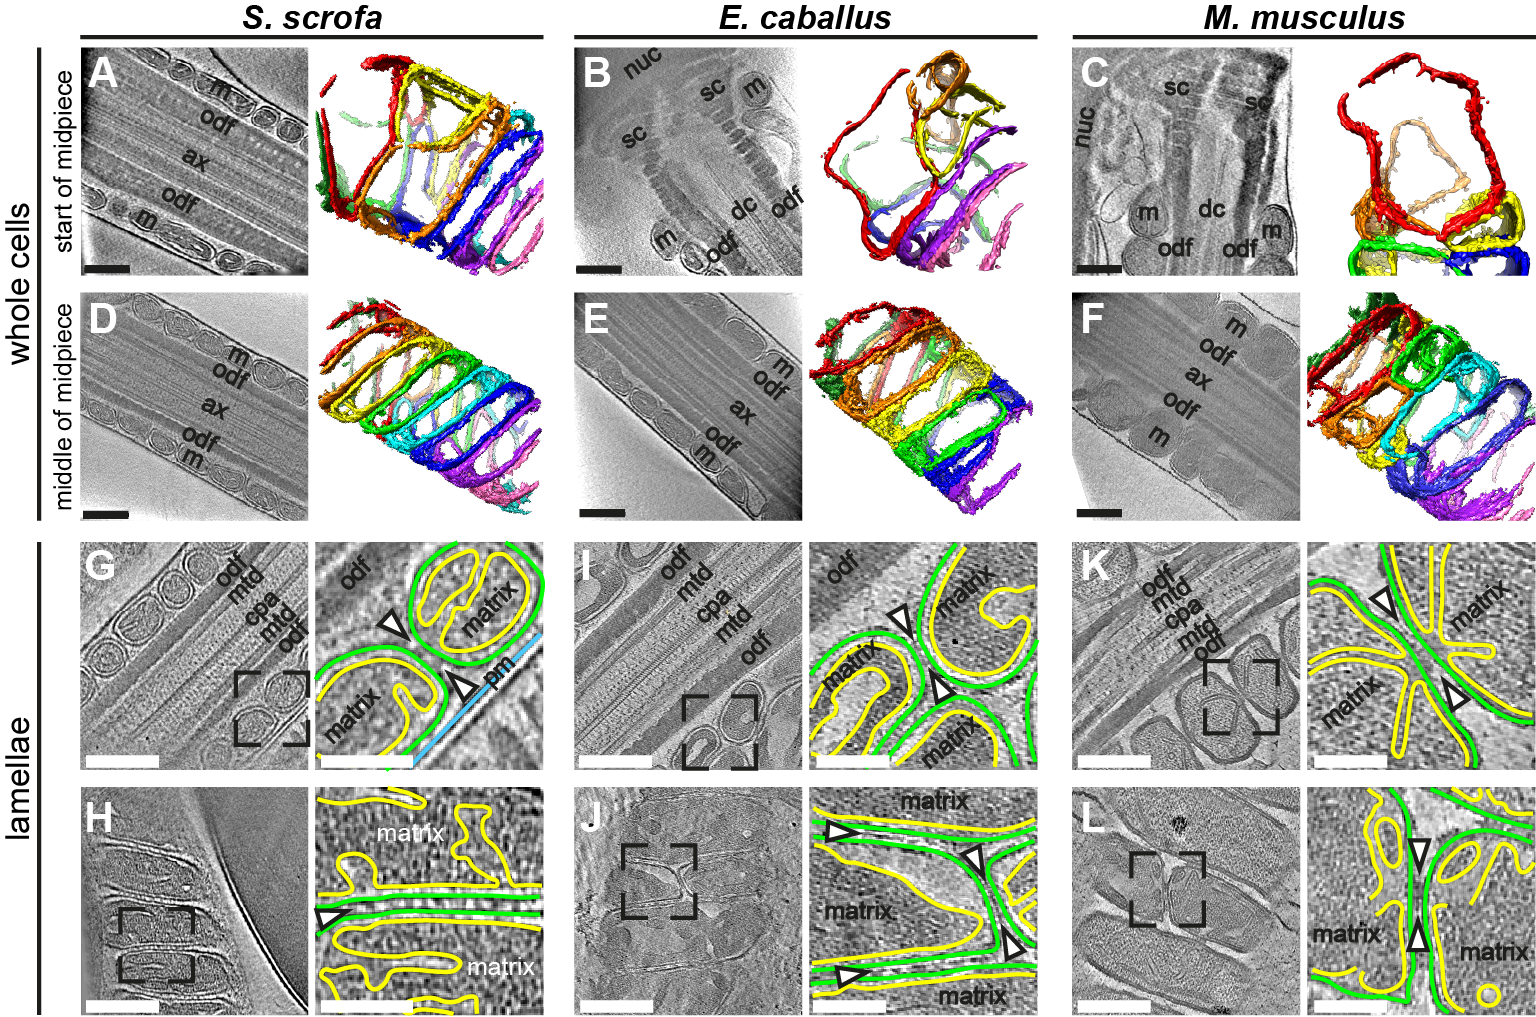
\includegraphics[]{Chapter.4/Figures/Figure1.png}
	\caption{\textbf{Mitochondrial dimensions and cristae organization vary across species.} \textbf{A-F.} Slices through Volta phase plate cryo-tomograms (left) and corresponding three-dimensional segmentations (right) of mitochondria from the start \textbf{A-C.} or middle \textbf{D-F.} of the midpiece from pig \textbf{A,D.}, horse \textbf{B,E.}, and mouse \textbf{C,F.} sperm. \textbf{G-L.} Slices through cryo-tomograms of FIB-milled pig \textbf{G,H.}, horse \textbf{I,J.}, and mouse \textbf{K,L.} sperm midpieces. Right panels show digital zooms of the regions boxed out in the left panels. The outer mitochondrial membrane is traced in green, the inner mitochondrial membrane in yellow, and the plasma membrane in blue. Arrowheads indicate inter-mitochondrial linker complexes. Labels: nuc - nucleus, sc - segmented columns, m - mitochondria, odf - outer dense fibers, dc - distal centriole, ax - axoneme, mtd - microtubule doublets, cpa - central pair apparatus, pm - plasma membrane. Scale bars: \textbf{A-L.} left panels - 250 nm, \textbf{G-L.} right panels - 100 nm.}
	\label{fig:ch4_fig1}
\end{figure*}
To visualize the internal organization of sperm mitochondria in a near-native state, we imaged sperm thinned by cryo-FIB milling (\textbf{\autoref{fig:ch4_fig1}G-L}). This revealed unexpected diversity in the internal ultrastructure of mitochondria across mammalian species, especially in terms of cristae morphology. Horse sperm mitochondria have an expanded intermembrane space and a condensed matrix (\textbf{\autoref{fig:ch4_fig1}I-J}). Mouse sperm mitochondria have an expanded matrix, with a narrow intermembrane space and thin cristae (\textbf{\autoref{fig:ch4_fig1}K-L}). Pig sperm mitochondrial morphology is intermediate (\textbf{\autoref{fig:ch4_fig1}G-H}), and although the mitochondrial matrix was dense, we could identify individual complexes that resembled ATP synthase on cristae of FIB-milled mitochondria (\textbf{\autoref{fig:ch4_app_fig2}A-B}), which was confirmed by subtomogram averaging (\textbf{\autoref{fig:ch4_app_fig2}B'}).

Inter-species differences in cristae morphology correlate with measurements of matrix volume relative to mitochondrial volume (\textbf{\autoref{fig:ch4_app_fig2}D}). In this regard, horse sperm mitochondria resemble “condensed” mitochondria, which correlate with higher rates of oxidative activity in a number of different cell types, including developing germ cells, neurons, and liver \cite{DeMartino1979, Perkins2011, Hackenbrock1968}. Indeed, horse sperm are dependent on oxidative phosphorylation \cite{Davila2016}, whereas pig \cite{Marin2003} and mouse sperm \cite{Mukai2004, Odet2013} are thought to rely largely on a glycolytic mechanisms.%\raggedbottom
%
\subsection*{Intermitochondrial junctions are associated with linker complexes}
Mitochondria are closely packed within the mitochondrial sheath, but it is unclear whether or how individual organelles communicate with their neighbors. To address this, we imaged intermitochondrial junctions captured in FIB-milled sperm lamellae. We observed trans-mitochondrial cristae alignment in mouse sperm\linebreak (\textbf{\autoref{fig:ch4_fig1}K-L}) (44/91 junctions across 14 tomograms), but not in pig or in horse sperm (\textbf{\autoref{fig:ch4_fig1}G-J}) (0/67 junctions across 11 tomograms and 0/41 junctions across 8 tomograms respectively). Trans-mitochondrial cristae alignment has also been observed in muscle tissue of various organisms, and is proposed to mediate electrochemical coupling between adjacent mitochondria \cite{Picard2015}. To our knowledge, this is the first time this phenomenon has been observed in mature sperm from any lineage. It is particularly curious, however, that trans-mitochondrial cristae alignment in sperm is species-specific.

We found that intermitochondrial junctions are characterized by novel intermitochondrial linker complexes in all three species (arrowheads in \textbf{\autoref{fig:ch4_fig1}G-L}, \textbf{\autoref{fig:ch4_app_fig2}C}). These intermitochondrial linkers span the $\sim$8-nm distance between the outer membranes of neighboring mitochondria. In mouse sperm, these linkers are specifically associated with sites of trans-mitochondrial cristae alignment\linebreak (\textbf{\autoref{fig:ch4_fig1}K-L}); in the pig and in the horse, they are positioned at regularly spaced intervals along intermitochondrial junctions (\textbf{\autoref{fig:ch4_fig1}I,J}). Electron-dense intermitochondrial junctions were also seen in cardiomyocytes by classical EM \cite{Huang2013, Picard2015, Duvert1985}. Thus, it is plausible that the as-yet-unidentified linker complexes we visualize here represent a more general structural mechanism for orchestrating intermitochondrial communication in various cell types.
%
\subsection*{Ordered protein arrays at the mitochondria-cytoskeleton interface are conserved across species}
To determine how mitochondria interact with the flagellar cytoskeleton, we imaged the mitochondria-cytoskeleton interface in cryo-FIB milled lamellae (\textbf{\autoref{fig:ch4_fig2}}). Previous studies using freeze-fracture EM on guinea pig sperm \cite{Friend1981} and mouse sperm \cite{Woolley2005}, and thin-section EM on golden hamster sperm \cite{Olson1992} uncovered an ordered array of particles arranged in a ladder-like pattern on the axoneme-facing surface of sperm mitochondria. We found these arrays on the axoneme-facing surface of the OMM in our tomograms as well (\textbf{\autoref{fig:ch4_fig2}A}, yellow box), across all three species and along the entire midpiece (\textbf{\autoref{fig:ch4_app_fig3}A-F}). We observed direct interactions between the arrays and either the ODFs or the cytoskeletal filaments surrounding the ODFs (\textbf{\autoref{fig:ch4_fig2}B-C}, \textbf{\autoref{fig:ch4_app_fig4}A-L}), indicating that these arrays tether mitochondria to the midpiece cytoskeleton. The highly-ordered arrays are absent from the plasma membrane-surface (\textbf{\autoref{fig:ch4_fig2}A}, red box), which is consistent with freeze-fracture EM studies that detect only very short rows scattered randomly across this surface \cite{Friend1981}.

We then aligned and averaged sub-volumes containing the protein arrays and the underlying OMM from the axoneme-facing surface (\textbf{\autoref{fig:ch4_fig3}}, \textbf{\autoref{tab:ch4_app_tab1}}). Our averages revealed $\sim$22-nm-long two-fold-symmetric boat-shaped structures connected via four densities to a porous membrane (\textbf{\autoref{fig:ch4_fig3}}, \textbf{\autoref{fig:ch4_app_fig3}G-I}).
\begin{figure*}[bt!]
	\center
	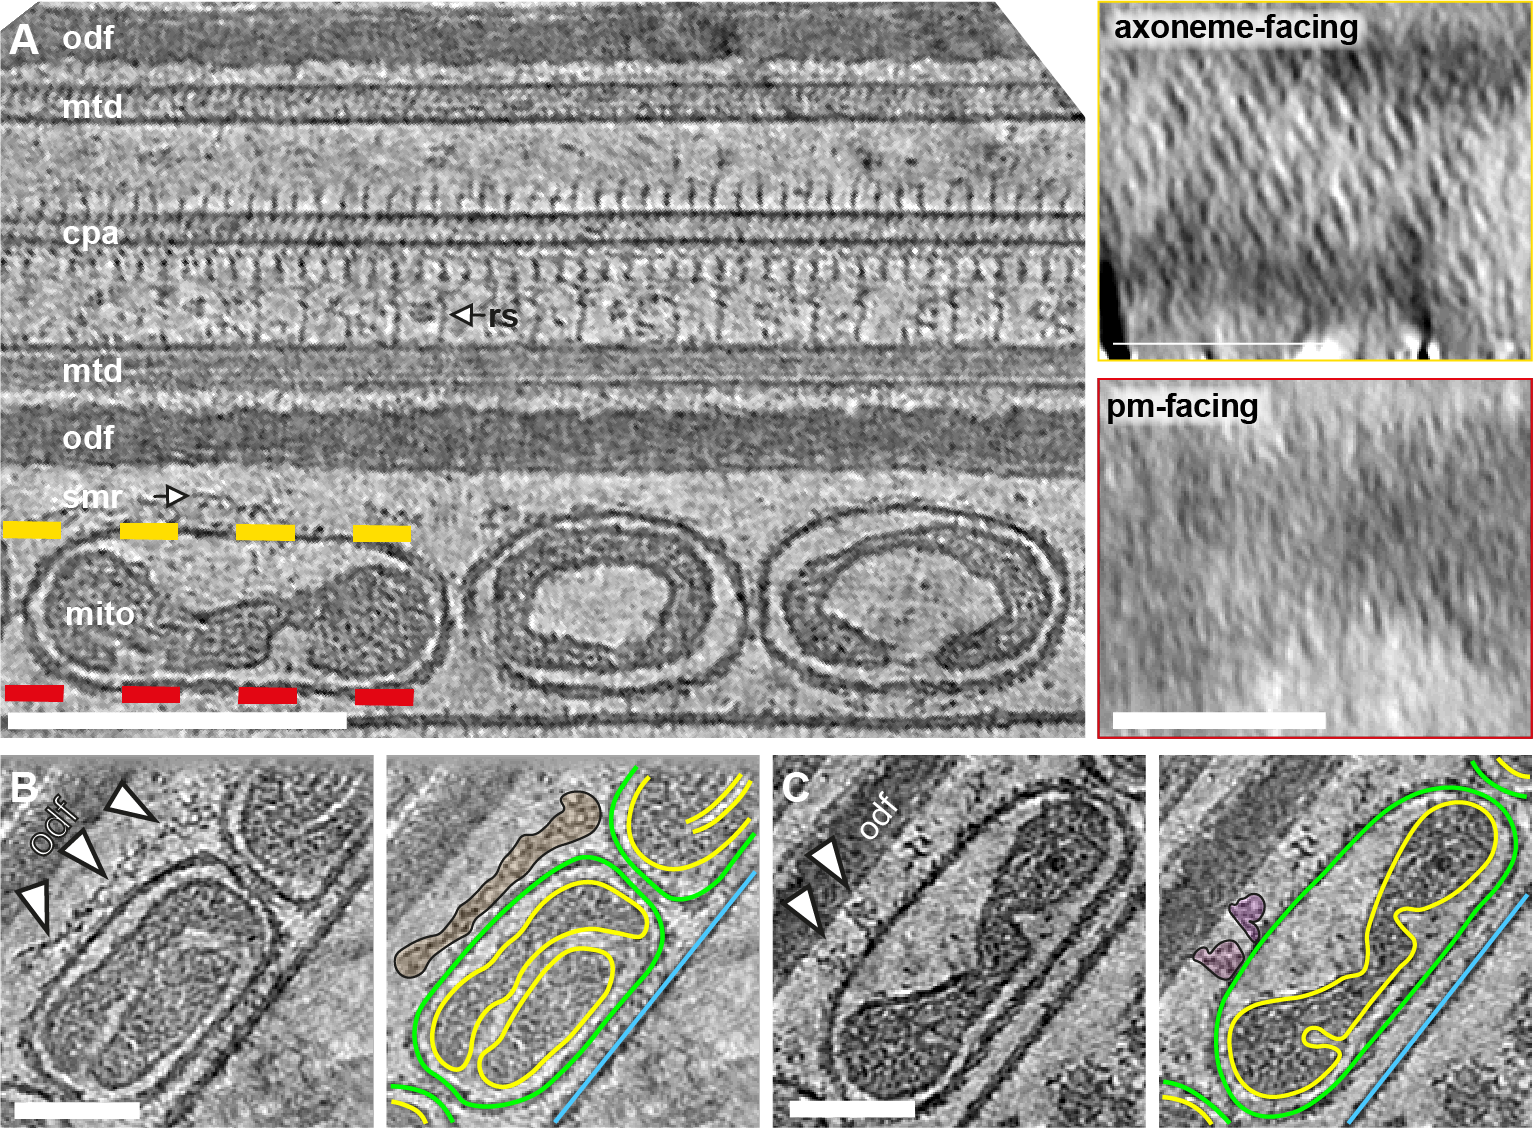
\includegraphics[]{Chapter.4/Figures/Figure2.png}
	\caption{\textbf{Ordered protein arrays on the outer mitochondrial membrane interact with the cytoskeleton.} \textbf{A.} Slice through a cryo-tomogram of a FIB-milled horse sperm midpiece, showing mitochondria (mito), the submitochondrial reticulum (smr) outer dense fibers (odf), microtubule doublets (mtd), and the central pair apparatus (cpa).  Note how individual complexes (like the radial spoke, rs) are visible in the raw tomogram. The ordered protein array is only found on the axoneme-facing surface (yellow) of midpiece mitochondria, and not on the plasma membrane-facing surface (red). \textbf{B,C.} Slices through a cryo-tomogram of a FIB-milled horse sperm midpiece showing how the array directly interacts with the submitochondrial reticulum to anchor mitochondria to the flagellar  cytoskeleton (arrowheads). In right panels, the outer mitochondrial membrane is traced in green, the inner mitochondrial membrane in yellow, and the plasma membrane in blue. Scale bars: \textbf{A.} left - 250 nm, insets - 100 nm; \textbf{B,C.} 100 nm.}
	\label{fig:ch4_fig2}
\end{figure*}
Each boat-shaped particle rises $\sim$5 nm above the membrane and consists of two tilde-shaped densities arranged end-to-end. The boat-shaped structures form rows in which each particle is related to its closest neighbors by a $\sim$10 nm translation perpendicular to the particle long axis and a $\sim$6 nm shift along this axis, yielding a center-to-center spacing of $\sim$12 nm (\textbf{\autoref{fig:ch4_fig3}D-F}). Each row is oriented $\sim$120° to the long axis of the flagellum and adjacent rows are spaced $\sim$12 nm apart, forming extensive arrays on the axoneme-facing surface of the OMM (\textbf{\autoref{fig:ch4_fig3}G}). Remarkably, the averages we obtained from the three species were highly similar, both in terms of individual particle dimensions and in terms of their supramolecular arrangement (\textbf{\autoref{fig:ch4_fig3}}, \textbf{\autoref{fig:ch4_app_fig3}}). This conservation suggests that these arrays are a crucial structural element of the mitochondrial sheath.

Our averages revealed that the OMM underlying the protein arrays is studded with $\sim$3-4 nm pores arranged in a pseudo-lattice with a center-to-center spacing of $\sim$5 nm. (\textbf{\autoref{fig:ch4_fig3}A-C}, \textbf{\autoref{fig:ch4_app_fig3}G-I}). These pore sizes are consistent with the diameters of the voltage dependent anion channels (VDACs), which are known to form ordered arrays in the OMM \cite{Guo1993, Hoogenboom2007, Goncalves2007, Mannella1982}. VDACs are known to localize to the sperm midpiece \cite{Kwon2013, Arcelay2008}; indeed, our label-free quantitative proteomics experiments show that VDAC2 and VDAC3 are among the most abundant OMM proteins in pig sperm (\textbf{\autoref{tab:ch4_app_tab2}}). Furthermore, the lattice dimensions in our averages closely match those of VDAC in purified Neurospora OMM \cite{Guo1993, Mannella1998}. The lattice can be modeled by fitting multiple copies of the VDAC2 crystal structure \cite{Schredelseker2014} (\textbf{\autoref{fig:ch4_app_fig5}A}). We oriented VDAC2 in the membrane plane based on its known topology \cite{Tomasello2013, Bayrhuber2008}; however, at the current resolution, we cannot determine the orientation around the pore axis. Thus, in our model, each boat-shaped particle stretches across 8 VDAC molecules (\textbf{\autoref{fig:ch4_fig3}}).

\begin{figure*}[tb!]
	\center
	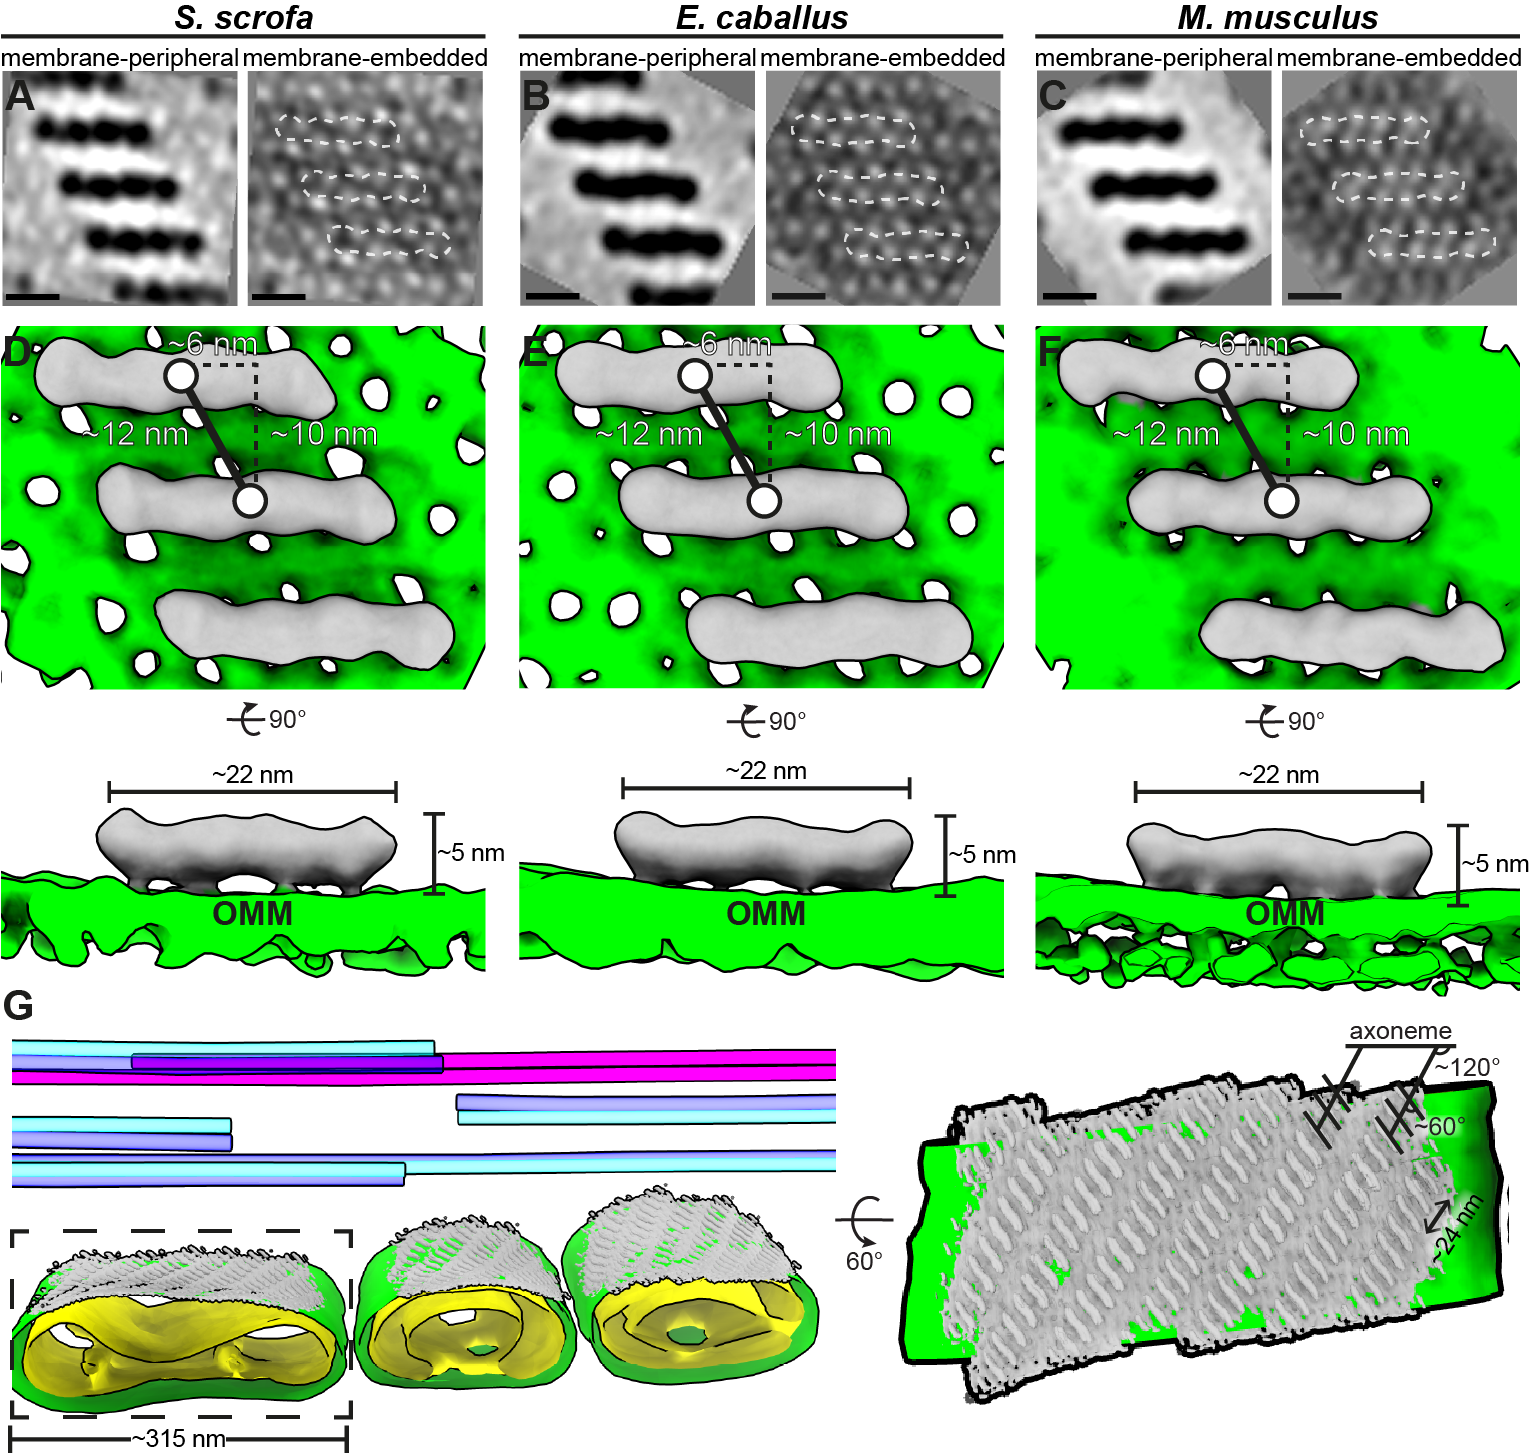
\includegraphics[]{Chapter.4/Figures/Figure3.png}
	\caption{\textbf{Ordered protein arrays at the mitochondria-cytoskeleton interface are conserved across species.} \textbf{A-C.} Subtomogram averages of the protein arrays and underlying outer mitochondrial membrane (OMM) after applying twofold symmetry (note that density is black). \textbf{D-F.} Isosurface renderings of the subtomogram averages in \textbf{A-C.} with boat-shaped particles in grey and the OMM in green. \textbf{G.} Left panel: Segmentation of the tomogram shown in Figure 2a, with the OMM in green, the IMM in yellow, microtubule doublets in blue, and the cpa in pink. Subtomogram averages of boat-shaped particles are colored grey and plotted back into their positions and orientations in the tomogram. Right panel: Rotated and zoomed-in view of the axoneme-facing surface of a mitochondrion. The axoneme is oriented horizontally, so the ladder-like arrays are oriented ~120° to the flagellar long axis, and individual particles within the array are oriented ~60° to this axis. Scale bars: \textbf{A-C.} 10 nm.}
	\label{fig:ch4_fig3}
\end{figure*}
%
\subsection*{Glycerol kinase-like proteins are probable constituents of the conserved arrays at the mitochondria-cytoskeleton interface}
To search for possible constituents of the protein arrays on the VDAC lattice, we used in-cell cross-linking mass spectrometry (XL-MS) \cite{Liu2018, Fasci2018} to find potential VDAC2 / VDAC3 interaction partners on the OMM (\textbf{\autoref{fig:ch4_fig4}}). We treated pig sperm cells with the cross-linker disuccinimidyl sulfoxide (DSSO), which covalently links free lysines that are within $\sim$3 nm (C$\alpha$-C$\alpha$) of each other. To increase confidence, we screened for protein interactions supported with at least two cross-link spectral matches (CSMs) (see Materials and Methods for details).

We first screened candidate proteins based on their known subcellular localizations (\textbf{\autoref{fig:ch4_fig4}A}). VDAC2/\linebreak VDAC3 cross-linked to mitochondria-associated proteins as well as to sperm head-associated proteins. This is consistent with immunofluorescence studies localizing VDAC2/VDAC3 both to the midpiece and to the acrosome, a large vesicle capping the anterior sperm nucleus \cite{Kwon2013, Hinsch2004, Arcelay2008}. Of the proteins in the mitochondria-associated interaction hub, four proteins are particularly noteworthy because they are known to localize to the OMM and because their disruption results in dysplasia of the mitochondrial sheath: armadillo repeat-containing protein 12 (ARMC12) \cite{Shimada2021}, spermatogenesis-associated protein 19 (SPATA19) \cite{Mi2015}, glutathione peroxidase 4 (GPX4) \cite{Schneider2009, Imai2009}, and glycerol kinase (GK) \cite{Chen2017a, Shimada2019}.

To distinguish among these candidates, we compared the location of the cross-links with the known topology of VDAC in the OMM \cite{Tomasello2013, Bayrhuber2008}. GPX4 would interact on the side facing the intermembrane space, whereas SPATA19, ARMC12, and GK would interact on the cytoplasmic face. Although we detect ARMC12 in mature pig sperm, in the mouse it is only present in developing spermatids and disappears from mature sperm \cite{Shimada2021}, which is inconsistent with the fact that the OMM arrays are present in cauda epididymal mouse sperm. SPATA19 and GK are both highly abundant (\textbf{\autoref{tab:ch4_app_tab2}}), as would be expected for proteins forming extensive arrays. Assuming an average protein density of $\sim$1.43 g/cm\textsuperscript{3} \cite{Quillin2000}, which corresponds to $\sim$0.861 Da/Å\textsuperscript{3}, we estimate that each boat-shaped particle in the array has a molecular weight of $\sim$250 kDa. SPATA19 is a small protein with an estimated molecular weight of $\sim$18 kDa. To fit into our EM densities, it must either be present in multiple copies or form a complex with other proteins. In contrast, GK has an estimated molecular weight of $\sim$60 kDa and is known to form S-shaped dimers ($\sim$120 kDa) that are conserved from bacteria \cite{Fukuda2016, Bystrom1999} to eukaryotes \cite{Balogun2019, Schnick2009}.

To build a GK-VDAC model based on our subtomogram average, we used rigid-body fitting to place two GK dimers end-to-end into a boat-shaped density (\textbf{\autoref{fig:ch4_app_fig5}B}, \textbf{\autoref{fig:ch4_fig4}B}). These fits defined a clear orientation for GK, with the N-termini pointing upwards and the C-terminal helices facing the OMM (\textbf{\autoref{fig:ch4_fig4}B}). To validate our fits, we mapped the cross-linked lysines onto the resulting model (\textbf{\autoref{fig:ch4_fig4}C}). All cross-links were between the cytosolic face of VDAC2 and the OMM-facing surface of GK, which is consistent with the orientation expected from our fits. These fits show that the molecular dimensions and relative positions of candidate proteins are consistent with our subtomogram average maps, but we cannot define specific interaction sites at the current resolution. We also attempted to analyze interactions between the putative GK-like proteins and the underlying cytoskeleton, and although we detect cross-links on the putative cytoskeleton-facing side of GK (\textbf{\autoref{fig:ch4_app_fig6}}), interpretation is complicated by the fact that the precise protein compositions of the submitochondrial reticulum and the ODFs are unclear.

Assigning GK-like proteins as constituents of the ordered OMM arrays at the mito\-chondria-cytoskeleton interface is also supported by recent genetic studies. Sperm from mice lacking sperm-specific GK isoforms have disorganized mitochondrial sheaths \cite{Chen2017a, Shimada2019}. In these mice, spherical mitochondria properly align along the flagellum but fail to properly elongate and coil around the flagellum, leaving gaps along the midpiece where the ODFs are exposed \cite{Shimada2019}. This phenotype is consistent with our data showing contacts between GK protein arrays and the underlying cytoskeleton (\textbf{\autoref{fig:ch4_fig2}B-C}, \textbf{\autoref{fig:ch4_app_fig4}S-L}), and by experiments showing that the submitochondrial reticulum remains attached to the OMM in detergent-extracted sperm (\cite{Olson1990}. Although sperm-specific GK isoforms do not show glycerol kinase activity in vitro \cite{Pan1999}, we cannot completely exclude that they function in mitochondrial metabolism \emph{in situ}, especially since knockout mice have higher ATP levels than wildtype (Chen2017a). If the arrays we observe indeed consist of GK-like proteins, and if these proteins are in fact metabolically active, then their preferential orientation towards the flagellar cytoskeleton could enhance metabolite shuttling between mitochondria and the axoneme.
\begin{figure*}[p]
	\center
	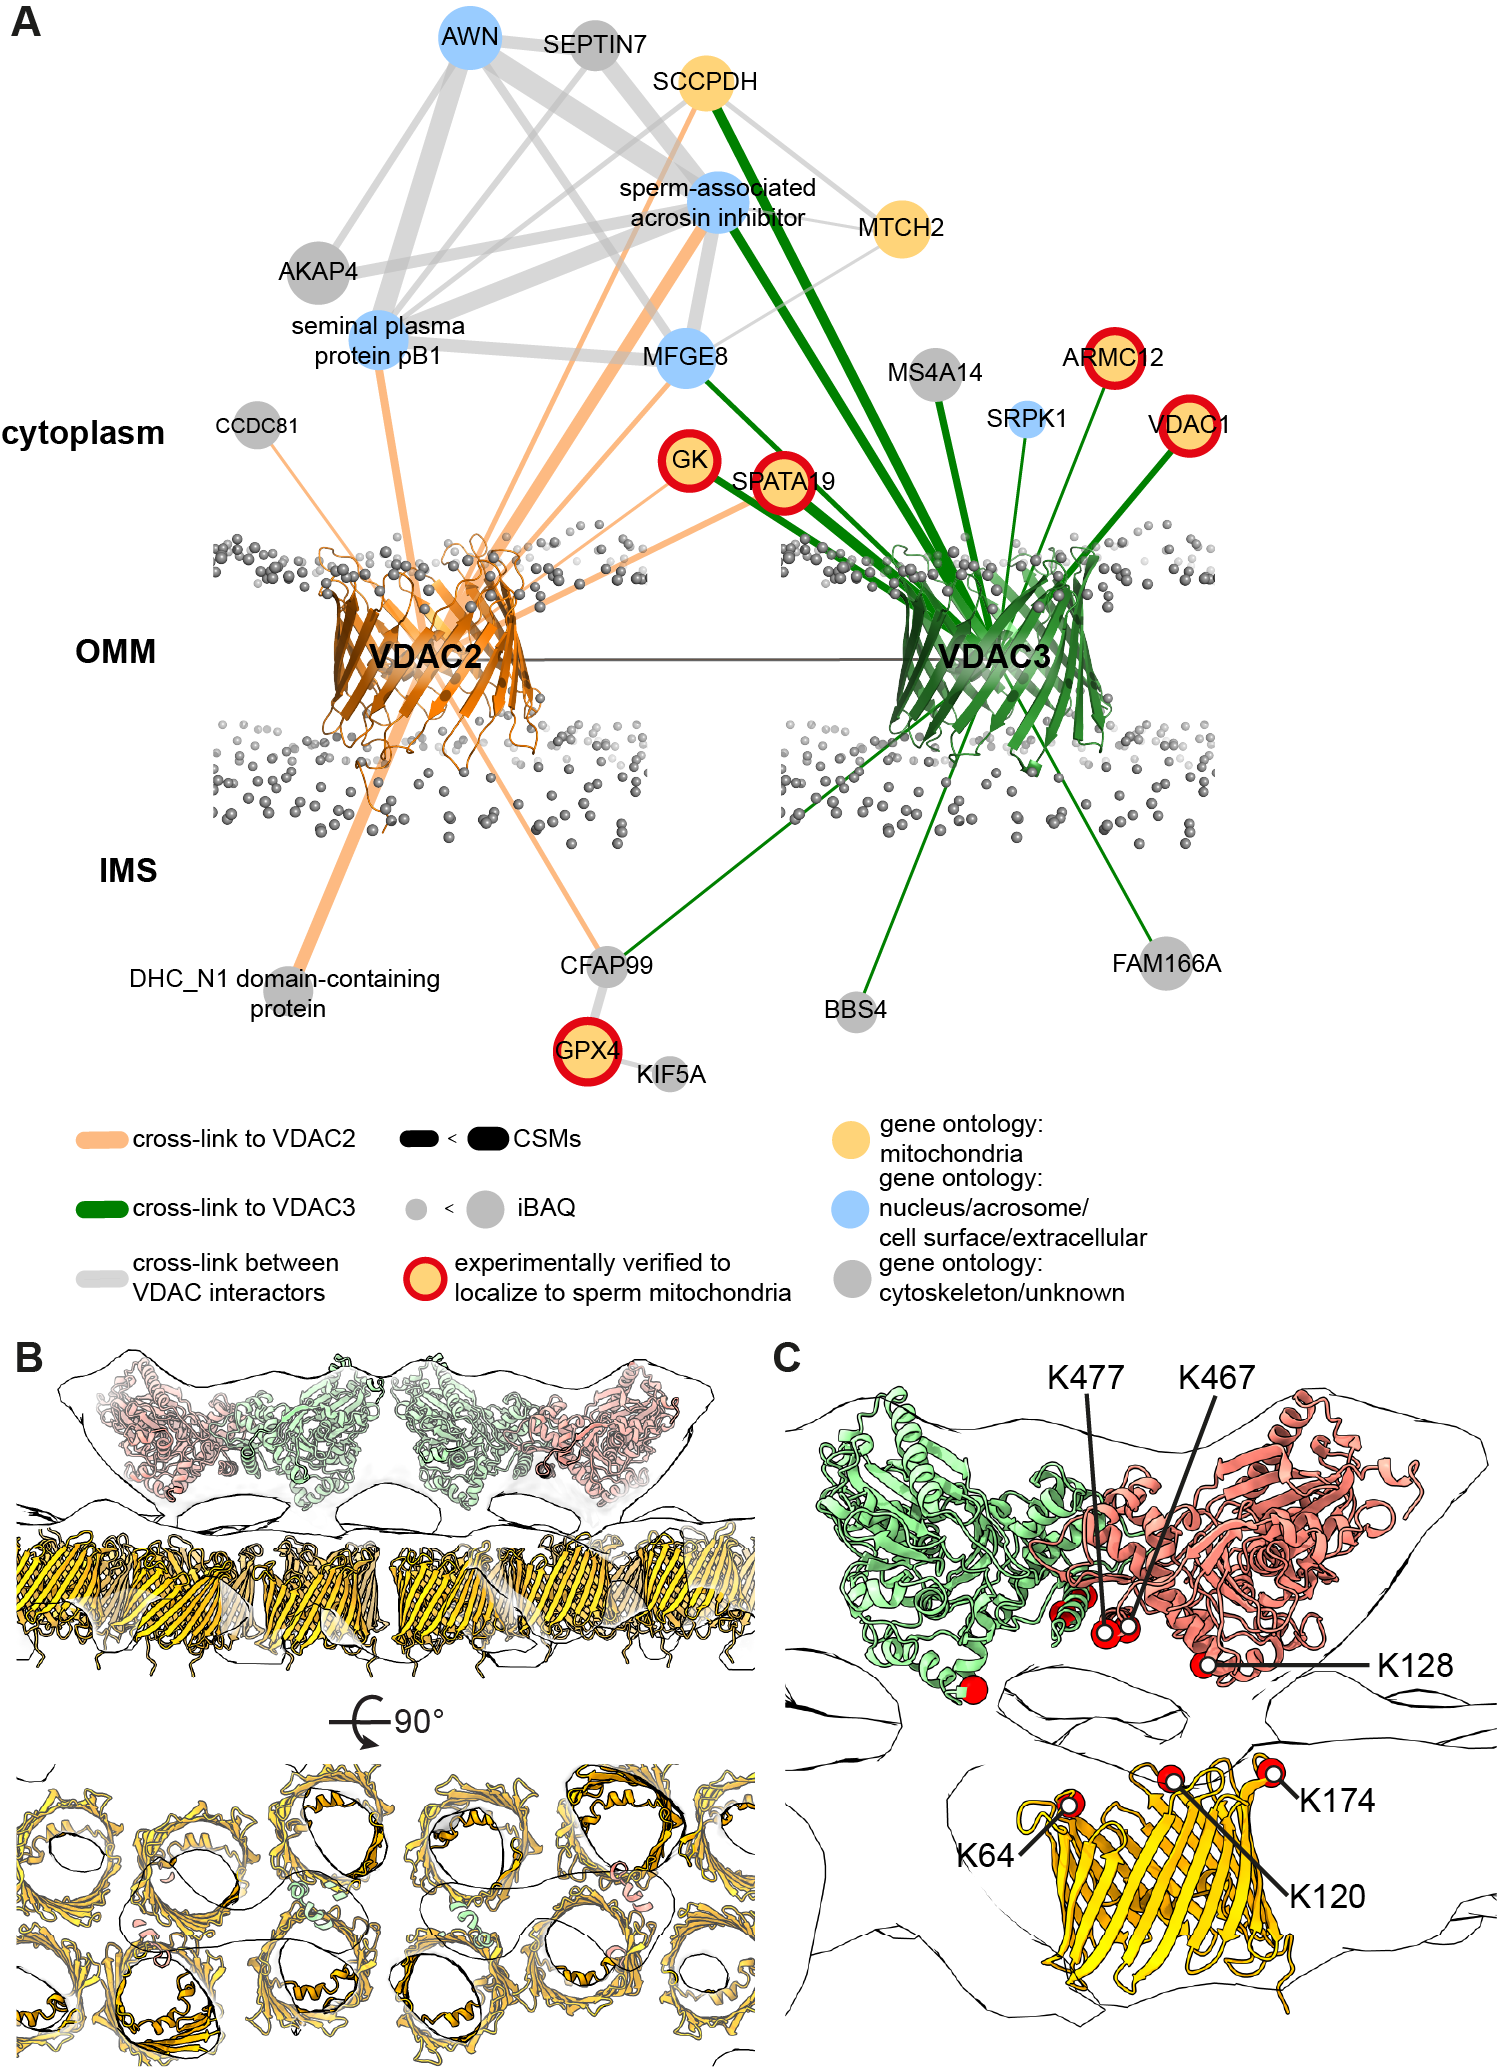
\includegraphics[]{Chapter.4/Figures/Figure4.png}
	\caption{Figure Legend on next page}
	\label{fig:ch4_fig4}
\end{figure*}
\addtocounter{figure}{-1}
\begin{figure*}[ht]
	\caption{\textbf{Modelling the outer mitochondrial membrane (OMM) array as glycerol kinase-like (GK) proteins anchored on voltage dependent anion channels (VDACs).} \textbf{A.} The VDAC2/VDAC3 interactome derived from in-cell XL-MS of pig sperm. Protein nodes are colored according to their known subcellular localizations (yellow with red border - experimentally verified to localize to sperm mitochondria; yellow - gene ontology: mitochondria, blue - gene ontology: nucleus/acrosome/cell surface; grey - gene ontology: cytoskeleton/unknown). Gray spheres indicate the phosphate groups of a simulated lipid bilayer which was structurally aligned based on the simulation for  monomeric mouse VDAC1 (PDB 4C69) obtained from the MemProtMD server \cite{Newport2019}. \textbf{B.} Modeling the OMM array as GK-like proteins anchored on VDACs. A GK-like dimer-of-dimers homology model (red and green) and VDAC2 homology models (yellow) were fitted into the pig subtomogram average map (white). \textbf{C.} The positions of cross-linked Lys residues (red circles) are consistent with GK and VDAC orientation assignments in our model. Note that the cross-links are shown for VDAC2, but we detect an additional cross-link between K140 on GK and VDAC3 (see \textbf{\autoref{fig:ch4_app_fig6}}).}
\end{figure*}
%
\section{Discussion}
In this study, we used cryo-FIB milling-enabled cryo-ET to image the sperm mitochondrial sheath in three mammalian species. Our data reveal that overall mitochondrial dimensions are remarkably consistent in sperm from the same species (\textbf{\autoref{fig:ch4_fig1}}, \textbf{\autoref{fig:ch4_app_fig1}}). This contrasts with other mitochondria-rich tissues such as muscle, where there are massive variations in mitochondrial size and morphology within individual cells \cite{Vincent2019}. In addition, we did not observe mitochondrial nanotunnels in any of the species we examined, in contrast to their relative abundance in muscle tissue \cite{Vincent2017, Vincent2019}. However, we do observe discrete linker proteins that tether neighboring mitochondria in all three species. It will be important to investigate the precise molecular identity of these linkers and to define whether they serve purely structural roles or also act as conducting channels that coordinate metabolite shuttling, energy production, and calcium signaling across the entire midpiece. Hinting at possible inter-organelle coordination, we observed trans-mitochondrial cristae alignment at specialized junctions between neighboring mitochondria in mouse sperm (\textbf{\autoref{fig:ch4_fig1}}). Thus, the concept of an interconnected mitochondrial reticulum that occurs in muscle \cite{Glancy2015} may also be applicable to the ma\-mmalian sperm midpiece and warrants further consideration.

In this study, we imaged either ejaculated or mature cauda epididymal sperm. However, mammalian sperm must undergo a plethora of biochemical and morphological changes in the female reproductive tract before they become fertilization-competent. These processes are collectively known as capacitation and cause extensive metabolic changes in sperm \cite{Mounib1964}. To cope with increased energy demands, rates of both glycolysis and oxidative phosphorylation increase during capacitation in mouse sperm \cite{Balbach2020}. Future work could use cryo-ET to establish whether these metabolic changes relate to any structural changes in midpiece mitochondria, for instance at the level of cristae architecture or intermitochondrial junctions.

Our data also show that mitochondrial dimensions and cristae architecture vary across species (\textbf{\autoref{fig:ch4_fig1}}), providing possible structural bases for interspecific differences in mitochondrial energetics. Horse sperm mitochondria appear to take on a more condensed appearance than their counterparts in pig and mouse, which may correlate with increased reliance on oxidative phosphorylation in horse sperm. Although studies on horse sperm physiology are limited \cite{Meyers2019}, condensed mitochondrial profiles are suggested to be a sign of calcium overload in other species \cite{Jamil1981, Okunade2004}, so cross-species studies exploring the link between mitochondrial morphology and possible differences in mitochondrial calcium homeostasis are clearly necessary.In general, the natural diversity of sperm enables comparative studies of how mitochondrial structure varies with sperm metabolism, which will undoubtedly contribute to our broader understanding of how mitochondrial form relates to function.

Our data show that, despite this diversity, the molecular underpinnings of mitochondrial sheath architecture are conserved, at least in mammals. Specifically, we identified novel intermitochondrial linkers that tether adjacent mitochondria (\textbf{\autoref{fig:ch4_fig1}}, \textbf{\autoref{fig:ch4_app_fig2}}). We also describe ordered protein arrays on the axoneme-facing surface of sperm mitochondria, which were first identified by freeze-fracture EM. Here, we characterize the three-dimensional architecture of these arrays in a near-native state and at molecular resolution, revealing how they are anchored on the OMM and how they interact with the flagellar  cytoskeleton. In-cell subtomogram averaging reveals that these arrays consist of boat-shaped particles anchored on a lattice of OMM pores (\textbf{\autoref{fig:ch4_fig2}}, \textbf{\autoref{fig:ch4_fig3}}). Proteomics and in-cell XL-MS suggest that these arrays consist of GK-like proteins anchored on VDAC lattices in the OMM (\textbf{\autoref{fig:ch4_fig4}}). Given that VDACs are ubiquitous OMM proteins, our findings motivate further efforts to explore whether they also regulate mitochondria-cytoskeleton interactions in other cell types.

The OMM arrays may function to regulate the precise elongation and coiling of mitochondria, contributing to the striking consistency within the mitochondrial sheath. In mature sperm, these arrays may help maintain the integrity of mitochondria-cytoskeleton contacts, stabilizing them against shear stresses during sperm motility and hyperactivation. However, it is unclear what determines the organization of these arrays in the first place. Our averages do not hint at direct interactions between boat-shaped particles. Instead, their spacing may be defined by the organization of the underlying VDAC lattice. Another intriguing possibility is that the arrays are organized by their cytoskeletal binding partners; the periodicity of relevant motifs on the submitochondrial reticulum could dictate the spacing of the OMM arrays.

We find that mitochondria-cytoskeleton contact sites in the sperm midpiece can be quite variable \linebreak (\textbf{\autoref{fig:ch4_app_fig4}}). Occasionally, OMM arrays make direct contact with the ODFs (\textbf{\autoref{fig:ch4_app_fig4}A-C,E-F,I}); sometimes, there are considerable gaps between them that are bridged either by the submitochondrial reticulum (\textbf{\autoref{fig:ch4_app_fig4}D,G-H,J}) or by unidentified linkers (\textbf{\autoref{fig:ch4_app_fig4}K-L}). This may be explained by variability in both the sizes and shapes of the ODFs themselves (\textbf{\autoref{fig:ch4_app_fig4}M-R}). Defining the precise mechanisms by which the OMM arrays tether to the underlying cytoskeleton is an important avenue for future research, in part because it has important implications for understanding sperm motility. In mammalian sperm, forces from axoneme bending are transmitted to the connecting piece through the ODFs, which are physically coupled to the microtubule doublets along most of the principal piece but not in the midpiece \cite{Lesich2014, Leung2021}. The observation that mitochondria are anchored to the ODFs through extensive ordered arrays adds another level of complexity to the multi-layered sliding mechanics of the mammalian sperm flagellum, affecting for example the extent to which the ODFs can slide relative to each other or to the axoneme. Indeed, the infertility of mice lacking sperm-specific GK isoforms appears to be caused by motility defects arising from the fragmented mitochondrial sheath \cite{Chen2017a, Shimada2019}. intermitochondrial linkers that physically tether neighboring mitochondria may also affect the extent to which the midpiece can bend during movement. On a larger scale, inter-species variations in mitochondrial dimensions and packing, coupled with known differences in overall midpiece length, could result in subtle changes in sperm motility. Furthermore, the stiffness of the midpiece changes during sperm maturation, becoming less rigid as sperm transit through the epididymis \cite{Jeulin1996, Miyata2015}. Tracing how the molecular structures we describe here form and change during spermiogenesis and epididymal maturation are likely to provide further insight in this respect. Ultimately, combining structural information from cryo-ET with motility analysis and mathematical modelling could help illuminate how midpiece morphometry affects swimming behaviour.

The methods we use here can also be used to study other specialized organelle configurations in the highly-streamlined sperm cell. For example, it is unclear how exactly the sperm head anchors to the tail, or how the acrosomal vesicle is laminated to the nucleus. Beyond sperm, such methods could be used to gain molecular insight into the organization of organelles in other terminally-differentiated and polarized cell types like neurons, photoreceptors, or hair cells. For example, exploring whether similar arrays are present at the mitochondria-cytoskeleton interface in other differentiated cell types - and whether they use a similar pool of protein components - is an area ripe for study. In striated muscle, proper mitochondrial positioning is critical for muscle function and depends on direct associations between mitochondria and intermediate filaments \cite{Konieczny2008, Milner2000}. Similarly, in skin cells, mitochondrial organization depends on keratin \cite{Steen2020}. The structural bases for these associations are unknown, but cryo-ET and in-cell XL-MS may prove useful in these contexts as well.
%%Material and Methods
\section{Materials and Methods}
\subsection*{Sperm collection and preparation}
Pig sperm samples were obtained from Varkens KI Nederland and prepared for imaging within a few hours of delivery. Sperm were layered onto a discontinuous gradient consisting of 4 mL of 35\% Percoll\textsuperscript{®} (GE Healthcare) underlaid with 2 mL of 70\% Percoll\textsuperscript{®}, both in HEPES-buffered saline (HBS: 20 mM HEPES, 137 mM NaCl, 10 mM glucose, 2.5 mM KCl, 0.1\% kanamycin, pH 7.6) and centrifuged at 750g for 15 min at room temperature (RT). Pelleted cells were washed once in phosphate-buffered saline (PBS: 137 mM NaCl, 3 mM KCl, 8 mM Na2HPO4, 1.5 mM KH2PO4, pH 7.4), and resuspended in PBS for further processing. All solutions were iso-osmotic at RT (290-300 mOsm/kg).

Horse semen was collected from mature Warmblood stallions using a Hanover artificial vagina in the presence of a teaser mare. Semen was filtered through gauze and kept at room temperature until further processing. Semen was diluted in INRA96 (IMV Technologies) to a sperm concentration of 30 x 106 cells/mL. Sperm were then centrifuged through a Percoll\textsuperscript{®} gradient (as described above for the pig) for 10 min at 300g followed by 10 min at 750g \cite{Harrison1993}. The pellet was resuspended in 1 mL of PBS, centrifuged for 5 min at 750g, and finally resuspended in PBS.

Mouse sperm were obtained from the cauda epididymis of adult male C57BL/6 mice as described in \cite{Hutcheon2017}. Male mice were culled as described in \cite{Mederacke2015} and the cauda epididymides were dissected with the vas deferens attached. Tissues were placed in a 500 µL droplet of modified Biggers, Whitten, and Whittingham media (BWW: 20 mM HEPES, 91.5 mM NaCl, 4.6 mM KCl, 1.7 mM D-glucose, 0.27 mM sodium pyruvate, 44 mM sodium lactate, 5 U/mL penicillin, and 5 µg/mL streptomycin, adjusted to pH 7.4 and an osmolarity of 300 mOsm/kg). Sperm were gently pushed out from the vas deferens, after which two incisions were made with a razor blade in the cauda. Spermatozoa were allowed to swim out of the cauda into the BWW over a period of 15 min at 37°C, after which the tissue was removed and sperm were loaded onto a 27\% Percoll\textsuperscript{®} density gradient and washed by centrifugation at 400g for 15 min. The sperm pellet was resuspended in BWW and centrifuged at 400g for 2 min to remove excess Percoll\textsuperscript{®}, then finally resuspended in BWW.
%
\subsection*{Cryo-EM grid preparation}
Typically, 3 µL of sperm suspension was pipetted onto a glow-discharged Quantifoil R 2/1 200-mesh holey carbon grid. Sperm cell density was approximately 2-3 x 106 cells/mL (for whole cell tomography) or 20-30 x 106 cells/mL (for cryo-FIB milling). One µL of BSA-conjugated gold (Aurion) was added, and the grids blotted manually opposite the side of cell deposition for $\sim$3 s (for whole cell tomography) or for $\sim$5-6 s (for cryo-FIB milling) using a manual plunge-freezer (MPI Martinsreid). Grids were immediately plunged into a liquid ethane-propane mix (37\% ethane) \cite{Tivol2008} cooled to liquid nitrogen temperature. Grids were stored under liquid N2 until imaging.
%
\subsection*{Cryo-focused ion beam milling}
Grids were mounted into modified Autogrids (ThermoFisher) for mechanical support. Clipped grids were loaded into an Aquilos (ThermoFisher) dual-beam cryo-focused ion beam/scanning electron microscope (cryo-FIB/SEM). SEM imaging was performed at 2 kV and 13 pA, whereas FIB imaging for targeting was performed at 30 kV and 10 pA. Milling was performed with stage tilts between 15° and 18°, so lamellae were inclined 8-11° relative to the grid.  Each lamella was milled in four stages: an initial rough mill at 1 nA beam current, an intermediate mill at 300 pA, a fine mill at 100 pA, and a polishing step at 30 pA. Lamellae were milled with the wedge pre-milling technique described in \cite{Schaffer2017} and with expansion segments as described in \cite{Wolff2019}.
%
\subsection*{Tilt series acquisition}
Tilt series were acquired on either a Talos Arctica (ThermoFisher) operating at 200 kV (all lamellae datasets and the whole-cell VPP horse dataset) or a Titan Krios (ThermoFisher) operating at 300 kV (whole-cell VPP pig and mouse datasets). Both microscopes were equipped with a post-column energy filter (Gatan) operated in zero-loss imaging mode with a 20-eV energy-selecting slit. All images were recorded on a K2 Summit direct electron detector (Gatan) in either counting or super-resolution mode with dose-fractionation. Tilt series were collected using SerialEM \cite{Mastronarde2005} at target defocus values between -4 and -6 $\mu$m (conventional defocus-contrast) or between -0.5 and -1.5 $\mu$m (for tilt series acquired with the Volta phase plate). Tilt series were typically recorded using either strict or grouped dose-symmetric schemes, either spanning ± 56° in 2° increments or ± 54° in 3° increments, with total dose limited to $\sim$100 e-/Å\textsuperscript{2}.
%
\subsection*{Tomogram reconstruction}
Frames were aligned either post-acquisition using Motioncor2 1.2.1 \cite{Zheng2017} or on-the-fly using Warp \cite{Tegunov2019}. Frames were usually collected in counting mode; when super-resolution frames were used (whole-cell VPP pig dataset), they were binned 2X during motion correction. Tomograms were reconstructed in IMOD \cite{Kremer1996} using weighted back-projection, with a SIRT-like filter \cite{Zeng2012} to aid visualization and segmentation. Defocus-contrast tomograms were CTF-corrected in IMOD using ctfphaseflip. VPP tomograms were left uncorrected.
%
\subsection*{Tomogram segmentation}
Segmentation was performed semi-automatically using the neural network-based workflow implemented in the TomoSeg package in EMAN 2.21 \cite{Chen2017b} Microtubules were traced manually in IMOD. Segmentation was then manually refined in Chimera 1.12 \cite{Pettersen2004} or in ChimeraX \cite{Goddard2018}. Visualization was performed in ChimeraX.
%
\subsection*{Subtomogram averaging of ATP synthase and ladder-like arrays}
Subtomogram averaging with missing wedge compensation was performed using PEET 1.13.0 \cite{Heumann2011, Nicastro2006} on defocus-contrast tomograms of cryo-FIB-milled lamellae. Resolution was estimated using the Fourier shell correlation (FSC) at a cut-off of 0.5 \cite{Nicastro2006}. Alignments were generally performed first on binned data, after which aligned positions and orientations were transformed to less-binned data using scripts provided by Dr. Daven Vasishtan. Details of acquisition parameters and particle numbers are summarized in \textbf{\autoref{tab:ch4_app_tab1}}.

Alignment strategies for mitochondrial complexes were designed to take advantage of their defined orientations relative to the membrane plane. Particles were picked manually and their initial orientations were defined using \emph{stalkInit}. Initial references were either a randomly chosen particle (for ladder-like arrays) or an average of all particles after roughly aligning them based on their initial orientations (for ATP synthase). Independent alignments using independent initial references were performed for datasets from different species. Alignments allowed for large rotational search ranges around the particle long axis (defined as the y-axis, perpendicular to the membrane plane), with limited search ranges around the x- and z-axes (the membrane plane).

All initial alignments were performed without symmetry. After visual inspection of the maps, twofold symmetry was applied for ladder-like arrays. Symmetrization involved using the aligned positions from the unsymmetrized runs as seed points and rotating particles around the axis of symmetry to generate virtual particles. A symmetrized volume was generated by averaging all particles and virtual particles and used as a reference for a final, restricted alignment.

Plotbacks were generated in IMOD by first running createAlignedModel to generate model files reflecting updated particle positions and orientations after alignment. The relevant subtomogram average was then thresholded for visualization and saved as an isosurface model, which was then placed back into the tomograms using \emph{clonemodel}.
%
\subsection*{Measurements and quantification}
All measurements of mitochondrial width were performed in IMOD on Volta phase plate tomograms filtered with a SIRT-like filter. Mitochondrial width was measured in the non-missing wedge direction at five points along the length of each mitochondrion. Only mitochondria that were entirely in the field of view were included in the measurements. Tomograms and corresponding measurements were then grouped based on their locations relative to the connecting piece, which were determined based on low-magnification images used for targeting during data acquisition. Internal mitochondrial ultrastructure was quantified from tomograms from cryo-FIB milled lamellae. The volume occupied by the matrix (V\textsubscript{\emph{matrix}}, the volume enclosed by the IMM) was measured relative to the volume occupied by the entire mitochondrion (V\textsubscript{\emph{mito}}, the volume enclosed by the OMM). Mesh volumes were extracted from segmentations using \emph{imodinfo}. Because neural network-based segmentation often resulted in gaps, mitochondrial membranes were segmented manually in IMOD for quantification. Only slices in which both the IMM and OMM were clearly defined were used for segmentation.
%
\subsection*{Cross-linking, lysis, digestion, and peptide fractionation}
All proteomics and cross-linking mass spectrometry experiments were performed on Percoll-washed pig sperm prepared as described above. For cross-linking, approximately 300 x 10\textsuperscript{6} cells were used, each from 3 different animals. Briefly, pelleted sperm cells were resuspended in 540 $\mu$L of PBS supplemented with disuccinimidyl sulfoxide (DSSO, Thermo Fisher Scientific) to a final concentration of 1 mM. The reaction mix was incubated for 30 min at 25°C with 700 rpm shaking in a ThemoMixer C (Eppendorf) and subsequently quenched for 20 min by adding Tris-HCl (final concentration 50 mM). Cross-linked cells were spun down at 13800g for 10 min at 4°C, after which the supernatant was removed. Cells were then lysed according to a protocol modified from \cite{Potel2018}. Cells were resuspended in 1 mL of lysis buffer (100 mM Tris-HCl pH 8.5, 7 M Urea, 1\% Triton X-100, 5 mM TCEP, 30 mM CAA, 10 U/ml DNase I, 1 mM MgCl\textsubscript{2}, 1\% benzonase (Merck Millipore, Darmstadt, Germany), 1 mM sodium orthovanadate, phosphoSTOP phosphatases inhibitors, and cOmpleteTM Mini EDTA-free protease inhibitors). Cells were sonicated on ice for 2 min using an ultrasonic processor (UP100H, Hielscher) at 80\% amplitude. The proteins were then precipitated according to \cite{Wessel1984} and the dried protein pellet resuspended in digestion buffer (100 mM Tris-HCl pH 8.5, 1\% sodium deoxycholate (Sigma-Aldrich), 5 mM TCEP, and 30 mM CAA). Trypsin and Lys-C proteases were added to a 1:25 and 1:100 ratio (w/w) respectively and protein digestion performed overnight at 37°C. The final peptide mixtures were desalted with solid-phase extraction C18 columns (Sep-Pak, Waters) and fractionated with an Agilent 1200 HPLC pump system (Agilent) coupled to a strong cation exchange (SCX) separation column (Luna SCX 5 $\mu$m - 100 Å particles, 50 x 2mm, Phenomenex), resulting in 25 fractions.
%
\subsection*{Liquid chromatography with mass spectrometry}
Approximately 1000 ng of peptides from each biological replicate before SCX fractionation were first injected onto an Agilent 1290 Infinity UHPLC system (Agilent) on a 50-cm analytical column packed with C18 beads (Dr Maisch Reprosil C18, 3 µm) coupled online to an Orbitrap HF-X (Thermo Fisher Scientific). For this classical bottom-up analysis, we used the following LC-MS/MS parameters: after 5 min of loading with 100\% buffer A (H2O with 0.1\% formic acid), peptides were eluted at 300 nL/min with a 95-min gradient from 13\% to 40\% of buffer B (80\% acetonitrile and 20\% H2O with 0.1\% formic acid). For MS acquisition we used an MS1 Orbitrap scan at 60,000 resolution, automatic gain control (AGC) target of 3 x 10\textsuperscript{6} ions and maximum inject time of 20 ms from 375 to 1600 m/z; the 15 most intense ions were submitted to MS2 Orbitrap scan at 30,000 resolution, AGC target of 1 x 10\textsuperscript{5} ions and maximum inject time of 50 ms (isolation window of 1.4 m/z, NCE at 27\% and dynamic exclusion of 16 seconds). The SCX fractions were analyzed with same Agilent HPLC and the same nano-column coupled on-line to an Orbitrap Lumos mass spectrometer (ThermoFisher Scientific). For these runs, we used a gradient from 6\% to 39\% buffer B over 100 min with specific MS settings for DSSO cross-links: survey MS1 Orbitrap scan at 60,000 resolution from 375 to 1500, AGC target of 4 x 10\textsuperscript{5} ions and maximum inject time of 50 ms; MS2 Orbitrap scan at 30,000 resolution, AGC target of 5 x 10\textsuperscript{4} ions, and maximum inject time of 100 ms for detection of DSSO signature peaks (difference in mass of 37.972 Da). The four ions with this specific difference were analyzed with a MS3 Ion Trap scans at AGC target of 2 x 10\textsuperscript{4} ions, maximum inject time of 150 ms for sequencing selected signature peaks (representing the individual peptides).
%
\subsection*{Data processing}
The 3 raw files obtained with classical bottom-up approach were analyzed with Max\-Quant version 1.6.17 with all the automatic settings adding Deamidation (N) as dynamic modification against the Sus scrofa reference proteome (Uniprot version of 08/2020 with 49,795 entries). With this search, we were able to calculate intensity-based absolute quantification (iBAQ) values and created a smaller FASTA file to use for analysis of cross-linking experiments. Raw files for cross-linked cells were analyzed with Proteome Discoverer software suite version 2.4.1.15 (ThermoFisher Scientific) with the incorporated XlinkX node for analysis of cross-linked peptides as described in \cite{Klykov2018}. Data were searched against the smaller FASTA created in house with “MS2\_MS3 acquisition strategy”. For the XlinkX search, we selected full tryptic digestion with 3 maximum missed cleavages, 10 ppm error for MS1, 20 ppm for MS2, and 0.5 Da for MS3 in Ion Trap. For modifications, we used static Carbamidomethyl (C) and dynamic Oxidation (M), Deamidation (N) and Met-loss (protein N-term). The crosslinked peptides were accepted with a minimum score of 40, minimum score difference of 4 and maximum FDR rate set to 5\%; further standard settings were used.
%
\subsection*{Interactome analysis, homology modelling, and cross-link mapping}
The interaction map for VDAC proteins was generated in R \cite{Grant2006} using the igraph package (v 1.2.4.2). Only protein interactions supported with at least two cross-link spectral matches (CSMs) were included in the final network. Homology models of pig GK and pig VDAC2 were generated in Robetta \cite{Kim2004} and fitted into subtomogram average maps by rigid body fitting in ChimeraX. Cross-links were mapped onto the resulting models using ChimeraX.
%
\subsection*{Data availability}
Subtomogram average maps have been deposited to the Electron Microscopy Data Bank (EMDB) with the following accession numbers: EMDB-12354, 12355, 12356, and 12357. The model of putative glycerol kinase-like proteins anchored on a VDAC array has been deposited to the Protein Data Bank (PDB) with the accession number PDB ID 7NIE. Mass spectrometry data have been deposited to the ProteomeXchange Consortium via the PRIDE partner repository with the dataset identifier PXD025562.
%
\subsection*{Acknowledgments}
The authors thank Dr. M Vanevic for excellent computational support; Dr. D Vasishtan for sharing scripts for subtomogram averaging; Ingr. CTWM Schneijdenberg and JD Meeldijk for managing the Utrecht University EM Square facility; Stal Schep (Tull en het Waal, The Netherlands) for providing horse semen; DVM MW Haaker and Dr. M Houweling for providing mouse reproductive tracts; Prof. F Förster and Prof. A Akhmanova for their comments on early versions of the manuscript; and Prof. EY Jones for insightful discussions. This work benefitted from access to the Netherlands Center for Electron Nanoscopy (NeCEN) with support from operators Dr. RS Dillard and Dr. C Diebolder and IT support from B Alewijnse. RZC, JFH, and AJRH acknowledge support from NWO funding the Netherlands Proteomics Centre through the X-omics Road Map program (project 184.034.019). This work was funded by NWO Start-Up Grant 740.018.007 to TZ. MRL is supported by a Clarendon Fund-Nuffield Department of Medicine Prize Studentship..
%
\subsection*{Author contributions}
PM, MZ, HH, EGB, and BMG provided sperm samples. MRL, MCR, and RTR prepared samples for cryo-ET. MRL performed cryo-FIB milling. MRL, MCR, RTR, SCH, and TZ collected cryo-ET data. MRL and MCR processed cryo-ET data. MRL, MCR, and TZ analyzed cryo-ET data. RZC and JFH performed all proteomics and cross-linking mass spectrometry experiments and corresponding structural modelling under the supervision of AJRH. MRL and TZ wrote the manuscript, and all authors contributed to revisions.
%
\subsection*{Conflict of interest}
The authors declare no competing interests.
\clearpage
%%Appendix
\begin{subappendices}
	%%Renew table numbering format
	\makeatletter\renewcommand{\thetable}{\thechapter.A.\@arabic\c@table}
	\makeatother
	\counterwithin{figure}{section}
	\section{Supplementary Material}
	\begin{figure*}[hbt]
		\center
		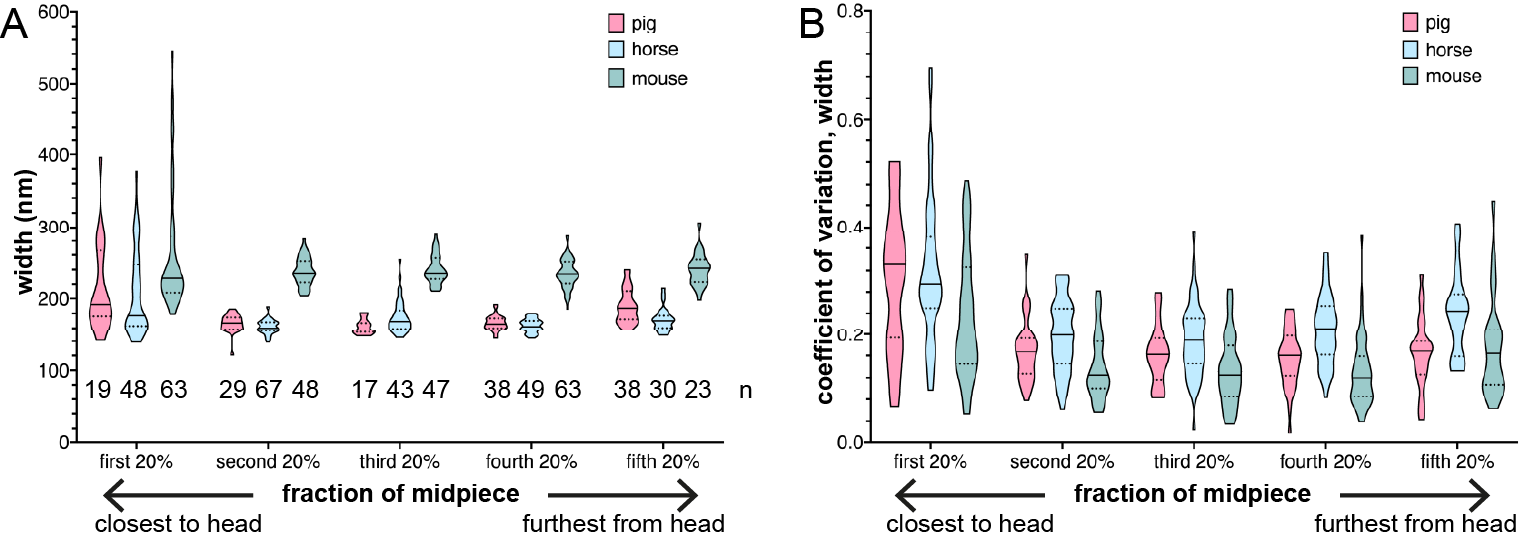
\includegraphics[]{Chapter.4/Figures/SI_Figure1.png}
		\caption{\textbf{Mitochondrial dimensions are consistent within species but vary across species and spatially along the midpiece.} \textbf{A.} Plotting the average width of mitochondria from different regions of the midpiece shows that mouse sperm mitochondria are larger than pig and horse sperm mitochondria. Note also that, in all three species, mitochondria at the proximal end of the midpiece are larger than those in more distal parts. \textbf{B.} Mitochondrial width was measured at five points along the length of each mitochondrion. Plotting the coefficient of variation from different regions along the midpiece shows that mitochondria at the start of the midpiece have more variable widths along their lengths. In \textbf{A.}, n indicates the number of mitochondria analyzed. In both \textbf{A.} and \textbf{B.}, solid lines represent the median and dotted lines represent the first and third quartiles.}
		\label{fig:ch4_app_fig1}
	\end{figure*}
	\begin{figure*}[hbt]
		\center
		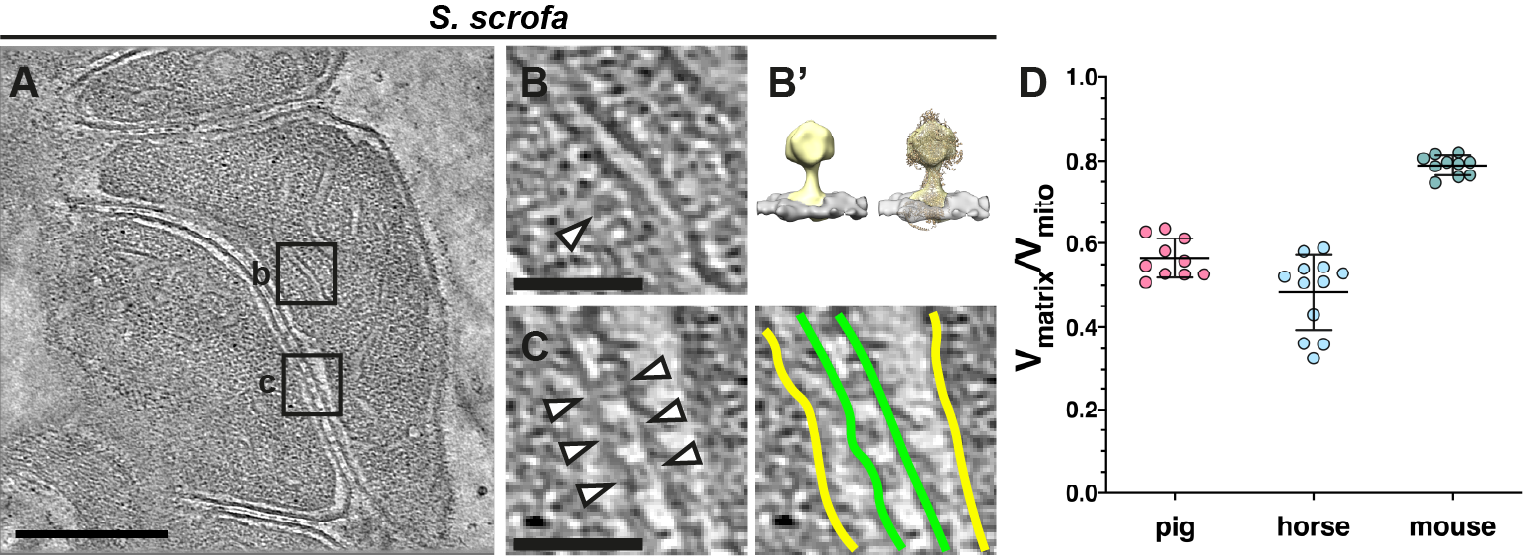
\includegraphics[]{Chapter.4/Figures/SI_Figure2.png}
		\caption{\textbf{Cryo-focused ion beam (cryo-FIB) milling reveals the internal organization of sperm mitochondria.} \textbf{A.} Slice through a cryo-tomogram of FIB-milled pig sperm mitochondria close to the connecting piece. \textbf{B.} ATP synthase can be directly identified on cristae based on its characteristic shape, which is confirmed by subtomogram averaging \textbf{B'}. \textbf{C.} Novel inter-mitochondrial linkers tether neighboring mitochondria to each other (arrowheads in left panel). \textbf{D.} Quantifying the volume enclosed by the mitochondrial matrix relative to the volume enclosed by the whole mitochondrion reveals that pig and horse sperm mitochondria have more expanded cristae and more condensed matrices than mouse sperm mitochondria. Lines represent mean ± standard deviation. Scale bars: \textbf{A.} 250 nm, \textbf{B-C.} 100 nm.}
		\label{fig:ch4_app_fig2}
	\end{figure*}
	\begin{figure*}[hbt]
		\center
		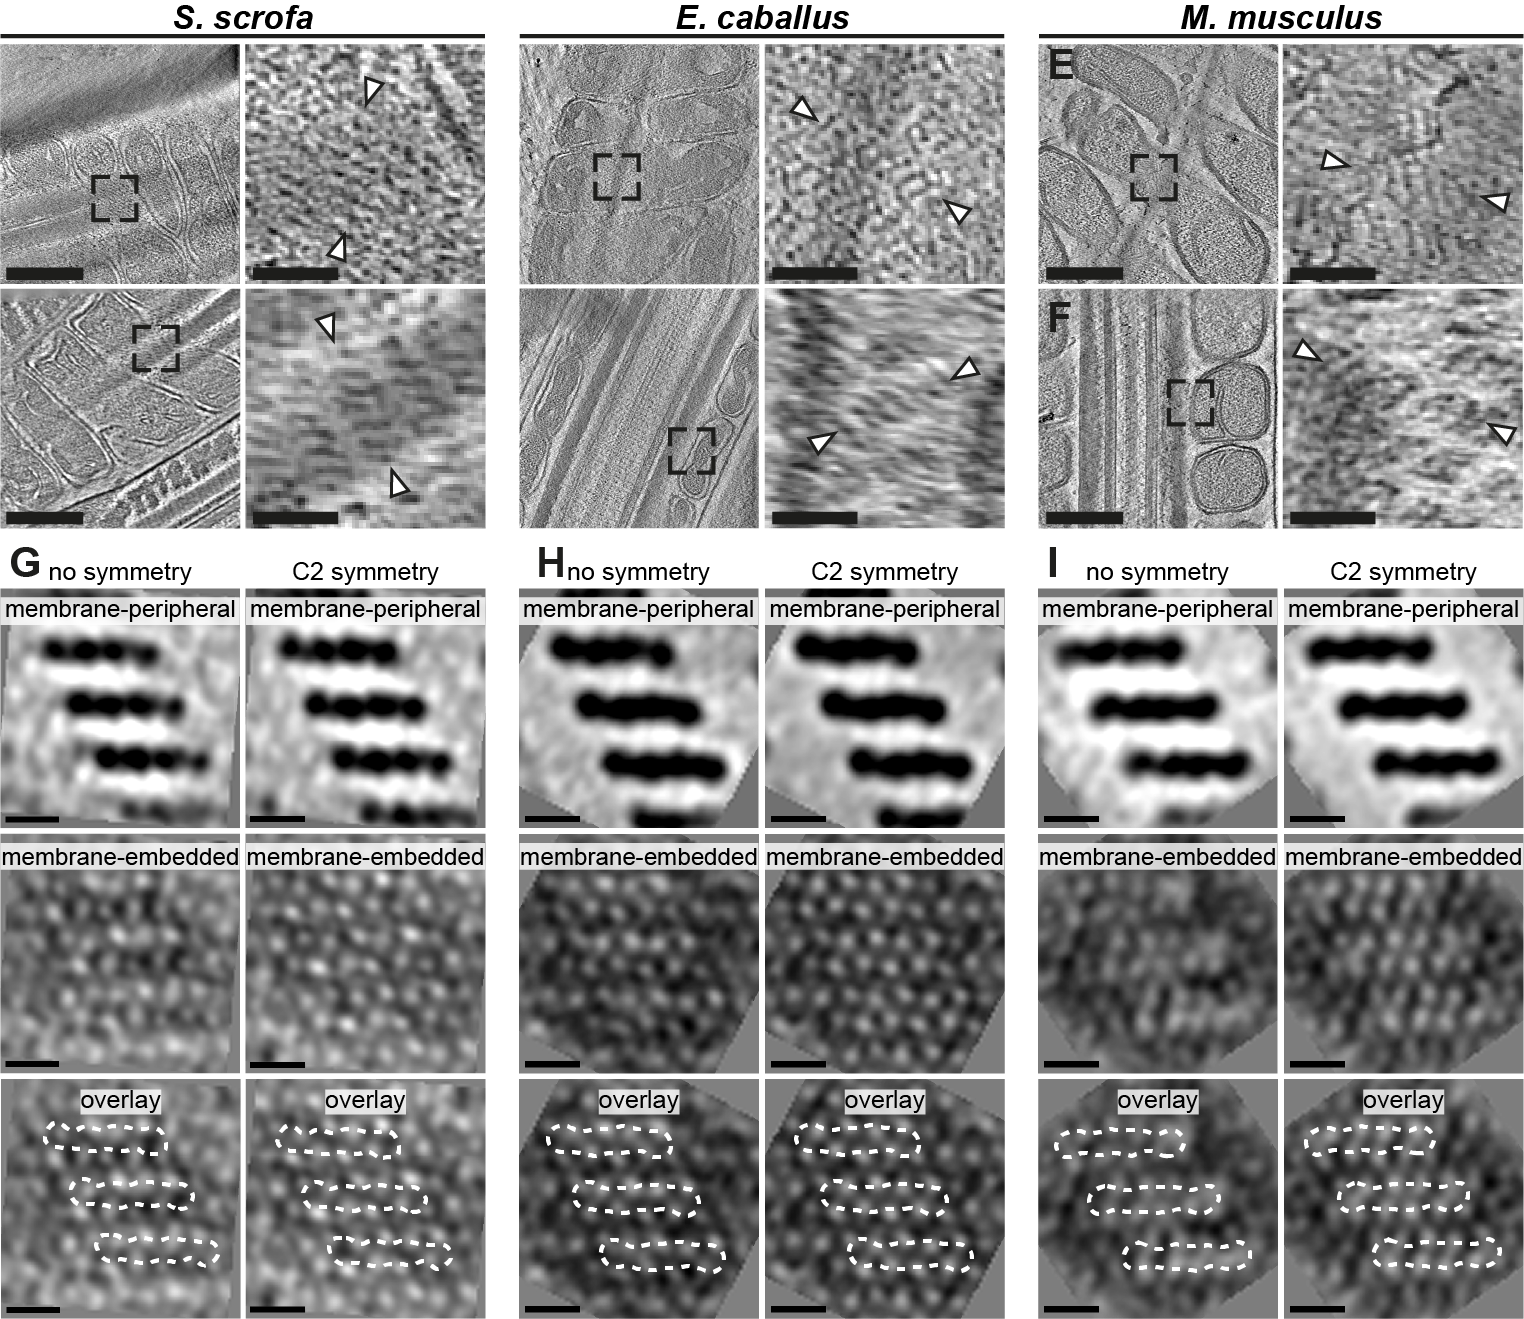
\includegraphics[]{Chapter.4/Figures/SI_Figure3.png}
		\caption{\textbf{The particles forming the ordered arrays at the mitochondria-cytoskeleton interface are two-fold symmetric.} \textbf{A-F.} Slices through cryo-tomograms of FIB-milled pig \textbf{A-B.}, horse \textbf{C-D.}, and mouse \textbf{E-F.} mitochondria. Right panels show digital zooms of the regions boxed out in the left panels, with arrowheads indicating arrays. \textbf{G-I.} Subtomogram averages of the arrays and the outer mitochondrial membrane (OMM) without (left) and with (right) twofold symmetry. Scale bars: \textbf{A-F.} 250 nm, \textbf{G-I.} 10 nm.}
		\label{fig:ch4_app_fig3}
	\end{figure*}
	\begin{figure*}[hbt]
		\center
		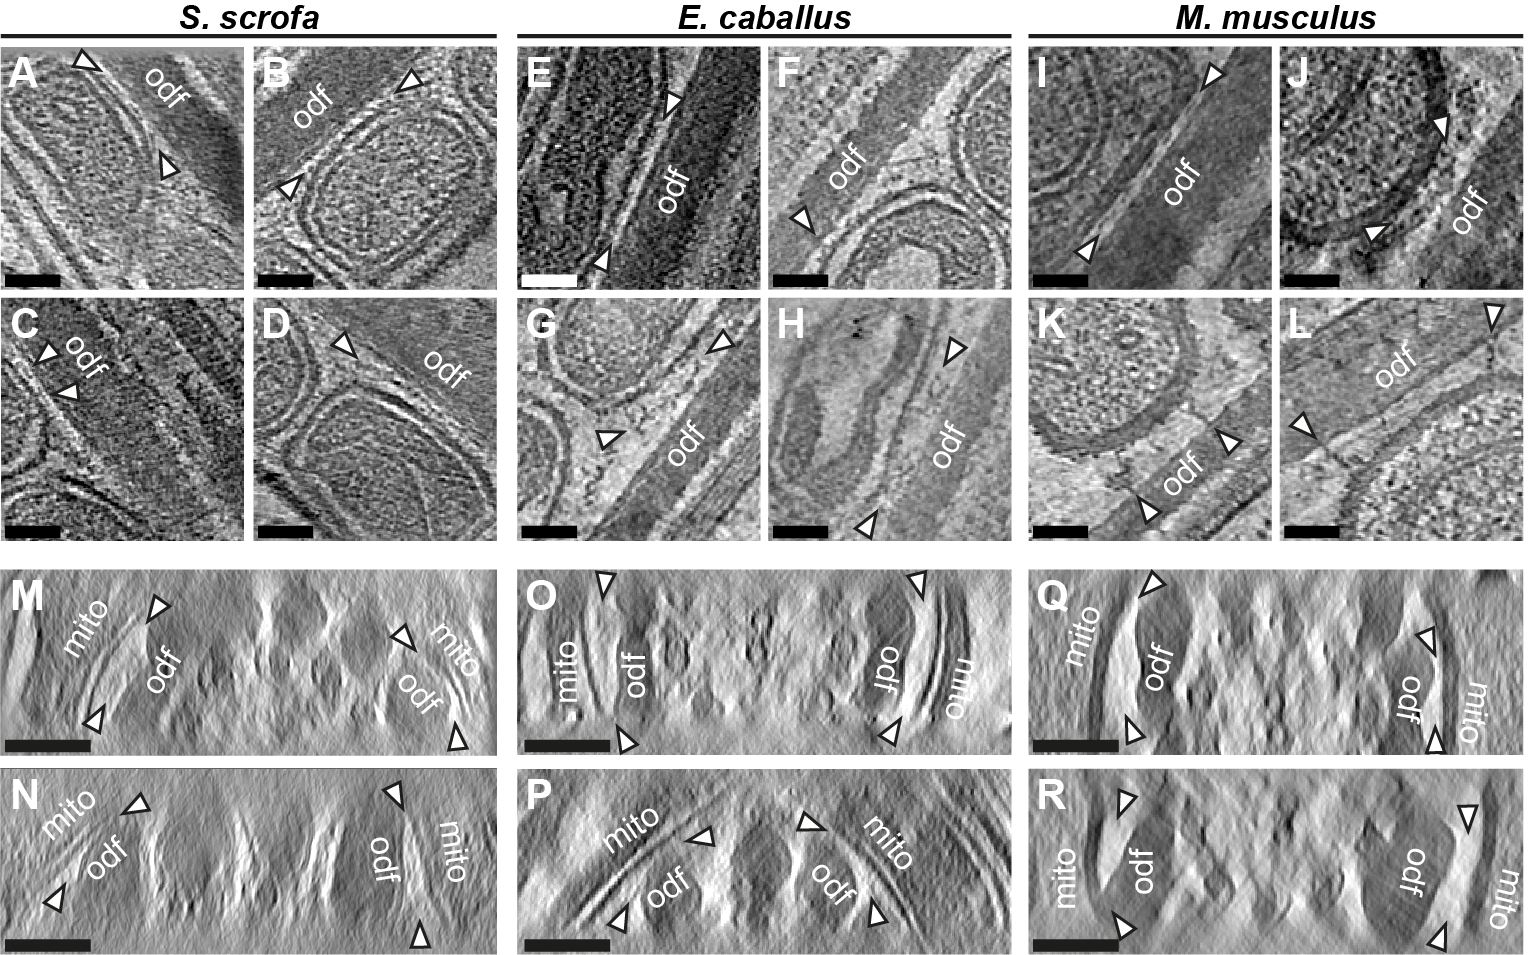
\includegraphics[]{Chapter.4/Figures/SI_Figure4.png}
		\caption{\textbf{Morphology of mitochondria-cytoskeleton contacts in the mammalian sperm midpiece.} \textbf{A-L} Slices through cryo-tomograms of FIB-milled pig (left), horse (middle), and mouse (right) sperm illustrating the variable nature of mitochondria-cytoskeleton contacts. Occasionally, the OMM array makes contact with the ODFs \textbf{A-C}, \textbf{E-F}, \textbf{I}; in other cases, the space between them is bridged by the submitochondrial reticulum \textbf{D,G-H,J} or by unidentified linkers \textbf{K-L}. \textbf{M-R} Transverse slices through cryo-tomograms illustrating how variability in size and shape of the outer dense fibers (ODFs) leads to variations in mitochondria-ODF spacing. Labels: odf - outer dense fiber, mito - mitochondria. Scale bars: \textbf{A-L} 50 nm, \textbf{M-R} 100 nm.}
		\label{fig:ch4_app_fig4}
	\end{figure*}
	\begin{figure*}[hbt]
		\center
		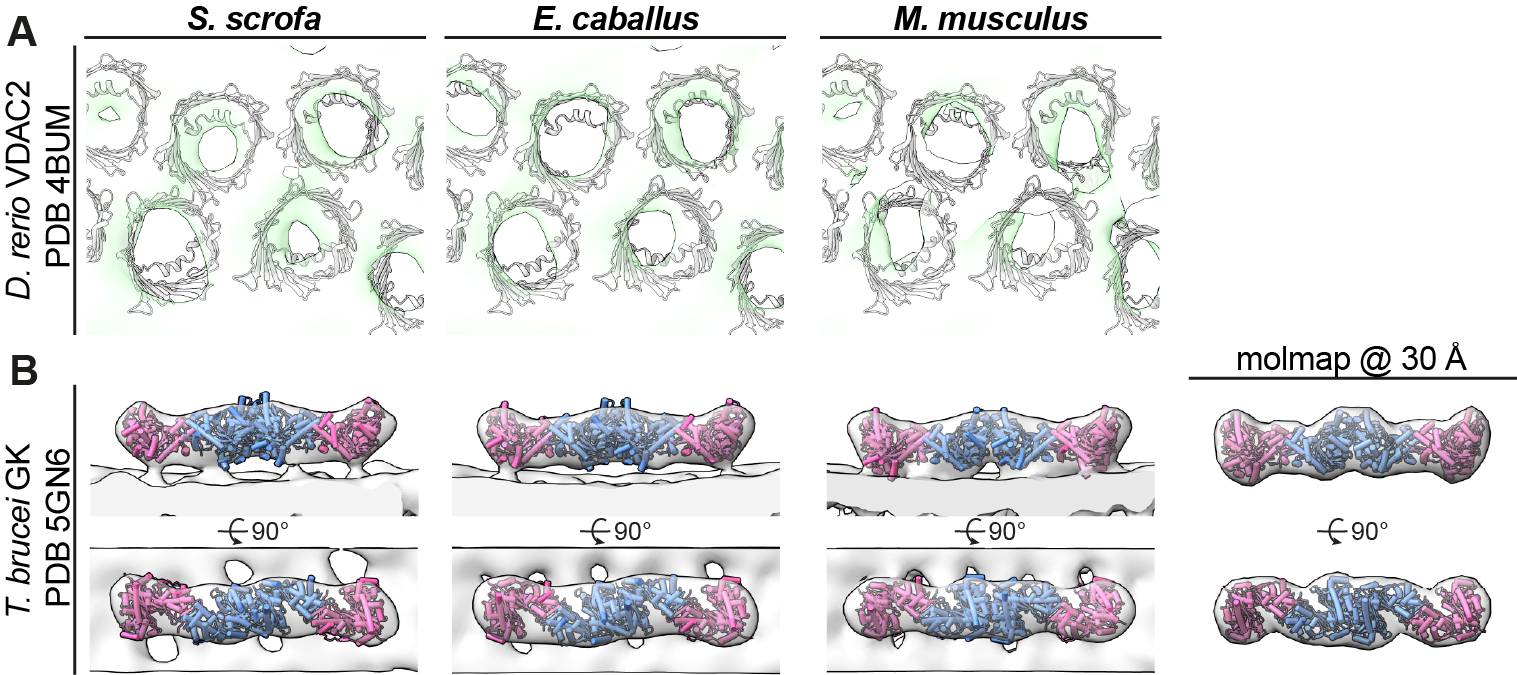
\includegraphics[]{Chapter.4/Figures/SI_Figure5.png}
		\caption{\textbf{Fitting crystal structures of glycerol kinase (GK) and voltage dependent anion channels (VDACs) into the pig subtomogram average map.} \textbf{A} The crystal structure of VDAC2 from zebrafish (PDB 4BUM) is shown in grey, fitted into the cryo-ET averaged map (green). \textbf{B} Two copies of a crystal structure of GK (pink and blue) from Trypanosoma brucei (PDB 5GN6) fitted into the cryo-ET averaged map (grey). On the right, the GK crystal structure is shown filtered to 30Å resolution.}
		\label{fig:ch4_app_fig5}
	\end{figure*}
	\begin{figure*}[hbt]
		\center
		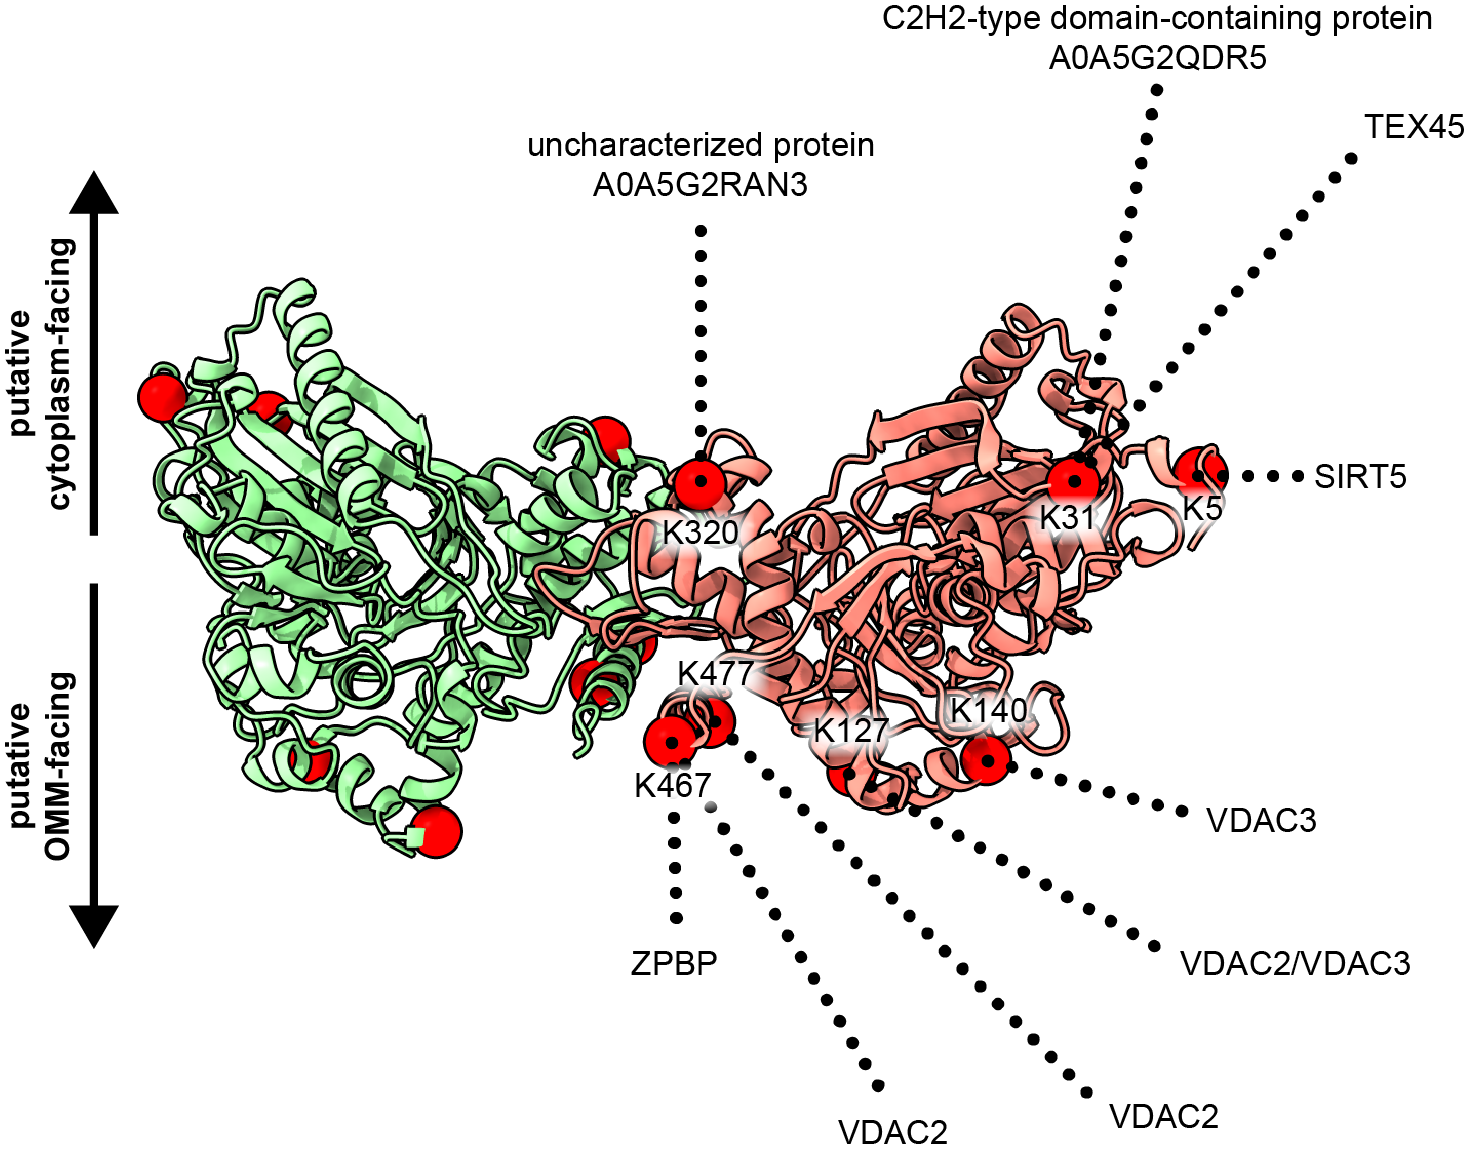
\includegraphics[]{Chapter.4/Figures/SI_Figure6.png}
		\caption{\textbf{The interactome of glycerol kinase (GK), a putative constituent of the boat-shaped particles on the ordered outer mitochondrial membrane array.} Each direct interaction partner of GK is connected by a dotted line to the lysine residue with which it cross-linked. Cross-linked lysine residues on GK are mapped onto a homology model of the pig GK dimer, which in turn is oriented based on our subtomogram average maps.}
		\label{fig:ch4_app_fig6}
	\end{figure*}
	\begin{table*}[hbt!]
		\caption{\textbf{Image acquisition and processing metrics for subtomogram averaging of mitochondrial protein complexes in mammalian
				sperm.}}
		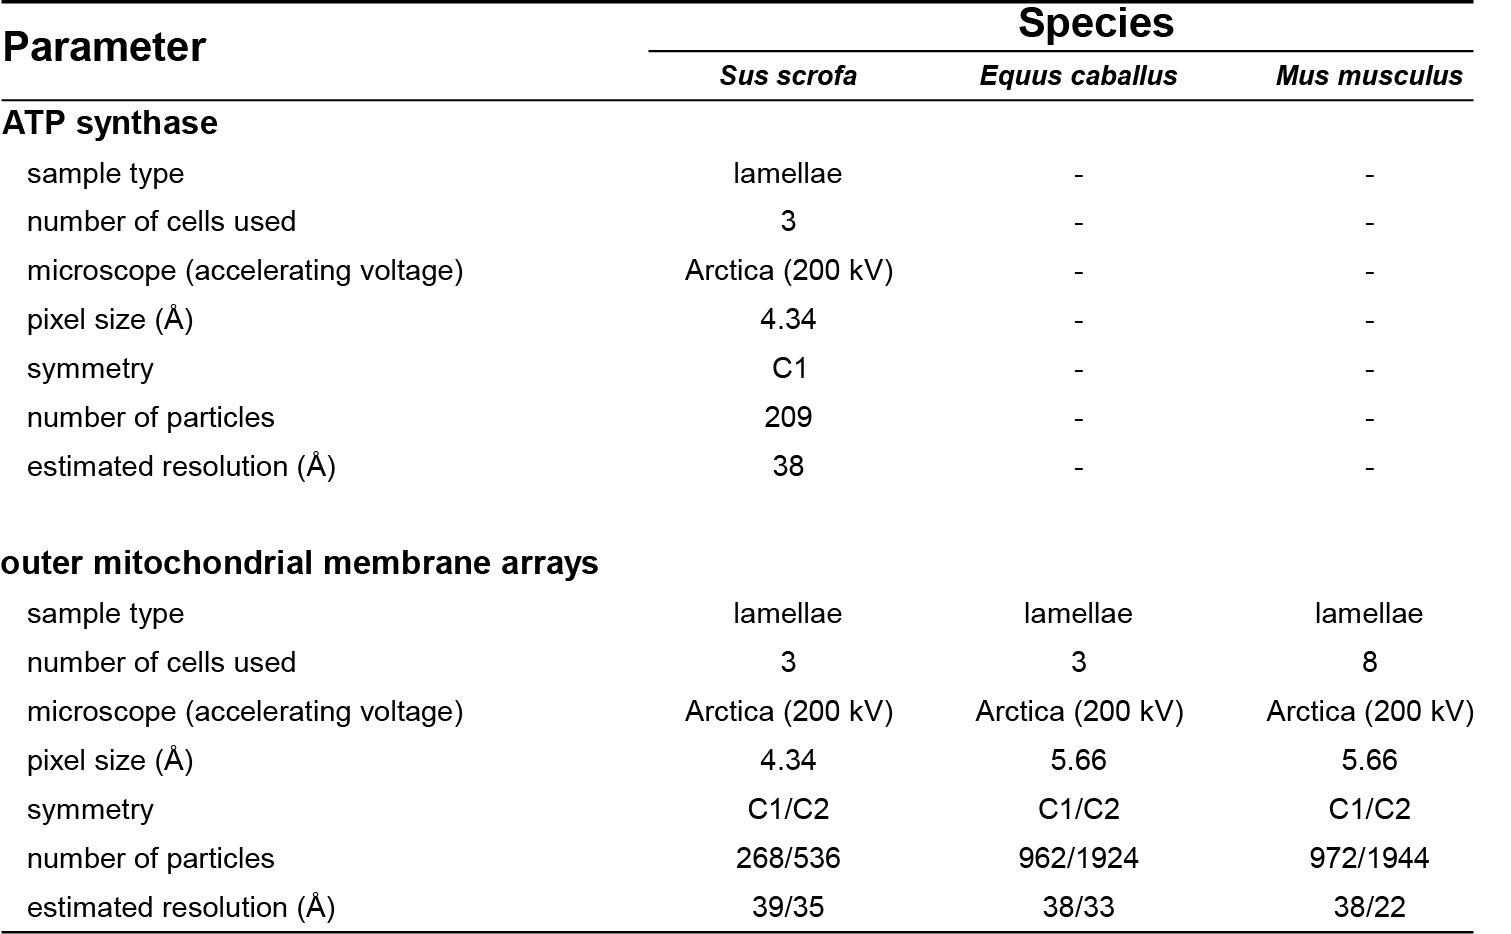
\includegraphics[]{Chapter.4/Figures/SI_Table1.png}
		\label{tab:ch4_app_tab1}
	\end{table*}
	\begin{table*}[hbt!]
		\caption{\textbf{Top 35 most abundant outer mitochondrial membrane proteins identified in the pig sperm proteome.}}
		\includegraphics[]{Chapter.4/Figures/SI_Table2.png}
		\label{tab:ch4_app_tab2}
	\end{table*}
\end{subappendices}
\clearpage
%%References
\section*{References}
\bibliographystyle{Style_settings/bibstyle_pnas}
\bibliography{Chapter.4/chapter4_bib}

%\picturechapter{MRPS36 provides a missing link in the eukaryotic 2-oxoglutarate dehydrogenase complex for recruitment of E3 to the E2 core}{Chapter_covers/chapter_cover_5.pdf} \label{ch-5}
\vspace*{0.25cm}

{\footnotesize Johannes F. Hevler, Pascal Albanese, Alfredo Cabrera-Orefic, Alisa Potter, Andris Jankevics, Jelena Misic, Richard A. Scheltema, Ulrich Brandt, Susanne Arnold and Albert J.R. Heck}
%
\begin{center}
    \vspace{3cm}
    \includegraphics[]{Chapter.5/Figures/OGDHC_schematic.png}
    \vspace{0.25cm}
\end{center}
%
\begin{flushleft}
    \vspace*{\fill}
    \rule{\textwidth}{1pt}\\[0cm]
    \textbf{This chapter is based on work in the following publication:}\\
    \footnotesize
    \textbf{\emph{bioRxiv}}, 2022.10.08.511390, doi:10.1101/2022.10.08.511390
\end{flushleft}
%
\begin{abstract102}
    The tricarboxylic acid (TCA) cycle, or Krebs cycle, is the central pathway of energy production in eukaryotic cells and plays a key part in aerobic respiration throughout all kingdoms of life. The enzymes involved in this cycle generate the reducing equivalents NADH and FADH2 by a series of enzymatic reactions, which are utilized by the electron transport chain to produce ATP. One of the pivotal enzymes in this cycle is 2-oxoglutarate dehydrogenase complex (OGDHC), which generates NADH by oxidative decarboxylation of 2-oxoglutarate to succinyl-CoA. OGDHC is a megadalton protein complex originally thought to be assembled just from three catalytically active subunits (E1o, E2o, E3). In fungi and animals, however, the protein MRPS36 has more recently been proposed as a putative additional component. Based on extensive XL-MS data obtained from measurements in mice and bovine heart mitochondria, supported by phylogenetic analyses, we provide evidence that MRPS36 is an essential member of OGDHC, albeit only in eukaryotes. Comparative sequence analysis and computational structure predictions reveal that in eukaryotic OGDHC, E2o does not contain the peripheral subunit-binding domain (PSBD), present in bacterial and archaeal E2o`s. We propose that in eukaryotes MRPS36 evolved as an E3 adaptor protein, functionally replacing the PSBD. We further provide a refined structural model of the complete eukaryotic OGDHC containing 16 E1o, 12 E3, and 6 subunits of MRPS36 accommodated around the OGDHC core composed of 24 E2o subunits (~3.45 MDa). The model provides new insights into the OGDH complex topology and stipulates putative mechanistic implications.
\end{abstract102}
%
\thumbforchapter
\section{Introduction}
\lettrine[lraise=0.1, nindent=0em, slope=-.5em]{T}{o} maintain all necessary biological tasks of life, organisms and cells are in a constant demand for energy \cite{Rigoulet_2020}. To satisfy those needs, cells consume energy-rich fuels in a series of complex energy-transforming processes. At the center of aerobic energy metabolism are the enzymes of the tricarboxylic acid (TCA) cycle, or Krebs cycle, which in eukaryotes are located within mitochondria \cite{Cavalcanti_2014,Martinez-Reyes_2020,Siriwat_2018}. The TCA cycle utilizes acetyl-CoA generated from sugars, fats and proteins in a series of enzymatic reactions to transfer electrons onto the reducing equivalents NADH and FADH2 \cite{Walsh_2018}. Subsequently, electrons are passed onto membrane bound respiratory chain protein complexes, fueling oxidative phosphorylation for the formation of adenosine triphosphate (ATP) \cite{Kaila_2021,Martinez-Reyes_2016}. Due to its central role in aerobic respiration, the TCA cycle has been extensively studied, resulting in a well-established view on enzymatic mechanisms and structural details of several of its enzymes \cite{Gleason_1994,Joyce_2000,Lauble_1992,Remington_1982,Spinelli_2018,Taylor_2008,Weaver_1996,Yankovskaya_2003}.

Because of its sheer size and multi-component nature, the 2-oxoglutarate dehydrogenase complex (OGDHC) is a less well characterized key enzyme of the TCA cycle. OGDHC is a member of the 2-oxo acid dehydrogenase (OADH) family, alongside with the pyruvate dehydrogenase complex (PDC) and the branched-chain $\alpha$-keto acid dehydrogenase complex (BCKDC). Each of these complexes consists of multiple copies of three catalytically active subunits (E1, E2, E3) assembling into multi-component enzymes weighing several megadaltons (MDa) that catalyze the oxidative decarboxylation of 2-oxo acids \cite{Reed_2001, Zhong_2022}. In contrast to E1 and E2, for which complex-specific genes exist (E1p/E1o/E1b, E2p/E2o/E2b), E3 is shared across all members of the OAHD complex family \cite{Nemeria_2021}. Eukaryotic PDC exhibits an icosahedral core composed of 60 E2p subunits and 12 copies of an additional non-catalytic E3-binding protein (E3BP), OGDHC and BCKDC contain an octahedral core that is solely formed by E2o and E2b subunits, respectively (\textbf{\autoref{fig:ch5_fig1}}). In all OADH complexes, E1 and E3 are thought to be arranged around the respective core, whereby the interaction involves a peripheral subunit-binding domain (PSBD) within E2. This relatively short (~35-residues) PSBD is composed of two parallel alpha-helices (H1, H2) connected by an extended loop \cite{Robien_1992}. Recruitment of E3 is mediated via charged side chains of H1 forming an electrostatic zipper \cite{Mande_1996}.

\begin{figure*}[t!]
    \centering
    \includegraphics[]{Chapter.5/Figures/Figure1.png}
    \caption{\textbf{Schematic overview of the three members of the 2-oxo-acid dehydrogenase complex (OADHC) family.} Pyruvate dehydrogenase complexes (PDC, left) contain an icosahedral E2p core to which E1p and E3 proteins become recruited. Additionally to E2p, PDC contains an alternative core forming subunit (E3BP) which specifically recruits E3. In contrast, for 2-oxoglutarate dehydrogenase complexes (OGDHC, middle) and branched-chain $\alpha$-keto acid dehydrogenase complex (BCKDC, right) E1 and E3 are tethered around an octahedral E2 core. For all three OADH members, peripheral subunit-binding domains (PSBD) in the E2 sequence (bottom row) have been proposed to play a key role in recruiting E1 and E3 subunits to the core \cite{Perham_2000}. For all family members, the lipoyl domain (LD) is essential for the carboxylation of 2-oxo acids, as it transfers respective intermediates from E1 to E2 components. Of these three, only OGDHC functions directly within the TCA cycle.}
    \label{fig:ch5_fig1}
\end{figure*}
In contrast to PDC and BCKDC, OGDHC functions directly within the TCA cycle metabolizing 2-oxoglutarate to succinyl-CoA, CO2 and NADH + H+ in three consecutive steps. First, 2-oxoglutarate is decarboxylated by thiamine pyrophosphate (TPP)-containing E1o (OGDH) and the respective 2-succinyl intermediate is transferred to the flexible lipoyl domain (LD) of E2o (DLST). Second, E2o transfers the succinyl functional group from its LD domain onto CoA-SH generating succinyl-CoA. In a final reaction, the LD domain of E2o is re-oxidized by E3 (DLD), a FAD-containing subunit that transfers electrons to NAD+ producing NADH \cite{Kyrilis_2021,Qi_2011}. While this catalytic mechanism is well understood, current structural insights into OGDHC lack detailed information about the complex architecture \cite{Frank_2007,Knapp_1998,Ricaud_1996,Robien_1992} in a close-to-native environment. Recent cryo-electron microscopic (cryo-EM) reconstructions of mammalian OGDHC revealed an octahedral core of 24 E2o subunits in an 8x3 assembly with E1o and E3 suggested to bind at the edges and faces, respectively \cite{Liu_2022,Nagy_2021}. Nonetheless, likely due to the highly conformational flexibility and possible heterogeneity of the complex \cite{Lengyel_2008}, these structures are not sufficient to understand how the E1o and E3 components are organized with respect to the core. MRPS36 (KGD4), a small (~11 kDa) and structurally unresolved protein, was more recently identified as a possible additional component of eukaryotic OGDHC \cite{Chatzispyrou_2018,Guerrero-Castillo_2021,Heublein_2014}. Its presence was suggested to be crucial for the efficient recruitment of E3 to the E2o core \cite{Heublein_2014}, but due to the lack of experimental evidence its function as an adaptor between E3 and the remainder of the OGDHC remains elusive. Also, in very recent high-resolution structural models of eukaryotic OGDHC, MRPS36 is not observed, or at least not reported on \cite{Liu_2022,Nagy_2021}.

Here, we explore the overall composition and architecture of mammalian OGDHC by combining complexome profiling (CP) \cite{Cabrera-Orefice_2021,Hevler_2021a} and cross-linking mass-spectrometry (XL-MS) with heart mitochondria from both mice and bovine origin. Based on the XL-MS and CP data and supported by phylogenetic analyses, we propose that MRPS36 is an essential member of OGDHC, albeit exclusively in eukaryotic mitochondria. Comparative sequence analysis reveals that MRPS36 replaces a functional domain, termed PSBD, that is preserved across prokaryotic E2o proteins and the other OADH complex members (PDC, BCKDC), but is absent in eukaryotic E2o. Based on our data and computational modeling, we provide a refined structural model of the eukaryotic OGDHC highlighting how E1o, E3 and MRPS36 are organized with respect to the core of E2o subunits and how they assemble into a functional complex of over ~3.45 MDa to act as a crucial component of the TCA cycle.
%
\section{Result and Discussion}
\subsection*{MRPS36 is a genuine member of OGDHC interacting with both the E2o core and E3}
To delve into the architecture of eukaryotic mitochondrial OGDHC and to verify the presence of MRPS36, we examined XL-MS data obtained from intact bovine heart mitochondria (BHM) \cite{Hevler_2021b} and murine heart mitochondria (MHM) (\textbf{Supplementary Table 1}). The here obtained XL-MS data for OGDHC of MHM were extended with previously published XL-MS data from our laboratory \cite{Liu_2018}. In both, mouse and bovine heart mitochondria, a substantial number of inter and intra-cross-links were observed for known members of the OGDHC (E1o, E2o, E3) and, notably, also for MRPS36. Our cross-linking experiments were more exhaustive for the BHM sample (as we applied three different chemical cross-linker reagents: DSSO, PhoX and DMTMM), resulting in a higher number of identified cross-links than for MHM (only cross-linked with DSSO). The observed cross-link patterns for all OGDHC subunits, including MRPS36, showed a high consistency between all technical and biological replicate datasets obtained from mitochondria of the two different organisms and by using different cross-linkers (\textbf{\autoref{fig:ch5_fig2}A}, \textbf{Supplementary Table 1}). On a separate note, we did not observe any cross-links between MRPS36 and mitochondrial ribosomal proteins, providing further evidence that its initial name as mitochondrial ribosomal protein S36, is indeed a misdemeanor. Several cross-links between all three components (E1o-E2o, E1o-E3, E2o-E3) were identified providing insights into the architecture of the binding interfaces within OGDHC. Our data showed that E1o interacts via its N-terminus and catalytic domain with both, a linker region (C-terminally of the LD-domain) and the catalytic domain of E2o. The involvement of respective regions in the formation of an E1o-E2o subcomplex as detected by XL-MS, is consistent with NMR and HDX-MS data reported for human OGDHC \cite{Zhou_2018}. Links between E1o and E3 components were also observed, albeit only in MHM, supporting previous findings that interactions between E1o and E3 are substantially weaker \cite{Zhou_2018}. Such weak E1o-E3 interactions could also hint at the absence of a stable subcomplex, which seems not surprising given that there is no direct dependency between the catalytic activities of E1o and E3. Our XL-MS data revealed stable interactions between residues of the LD-domain of E2o with the adjacent flexible linker region and the FAD/NAD binding domain of E3. In bacterial PDC and OGDHC, E3 is recruited to the E2 core via the PSBD of E2 \cite{Frank_2005, Fries_2007, Mande_1996, Perham_2000, Robien_1992}. For eukaryotic OGDHC, such an E2-PSBD was postulated and proposed to be located in the flexible linker region, C-terminal to the LD-domain \cite{Liu_2022}. However, so far, there has been no evidence found corroborating this assumption.

\begin{figure*}[p]
    \centering
    \includegraphics[]{Chapter.5/Figures/Figure2.png}
    \caption{\textbf{Exploring the architecture of eukaryotic OGDHC using XL-MS and CP.} \textbf{A.} Circos plots showing intra and inter cross-links for members of OGDHC from bovine heart mitochondria (BHM, left) and mouse heart mitochondria (MHM, right). BHM were cross-linked with three different chemical cross-linkers (DSSO, PhoX and DMTMM) providing Lys-Lys and Lys-Asp/Glu cross-links. MHM were only cross-linked by using DSSO providing Lys-Lys cross-links. Cross-links for MHM were merged with previously published data from our lab \cite{Liu_2018}. Functional domains are highlighted as colored tracks and were annotated using Interpro \cite{Blum_2021}. Cross-linkable residues are indicated in a separate track. Depending on whether they are engaged in a cross-link they are either black (not cross-linked) or colored (involved in a cross-link) with Lys residues color-coded green and Asp and Glu orange. Sequences for E1o, E2o and E3 include mitochondrial transit peptides \textbf{B.} Migration profiles of bovine OGDHC subunits from non-cross-linked (untreated) and cross-linked (PhoX or DMTMM) heart mitochondrial samples separated by BN-PAGE (3 to 10\%). MRPS36 is found to co-migrate with E1o, E2o, E3 subunits of the OGDHC. Peaks are annotated based on the apparent molecular masses of monomeric E1o (~111 kDa), monomeric E2o (~41 kDa), monomeric E3 (~50 kDa) and monomeric MRPS36 (11 kDa). Cross-linking seems to stabilize binding of E3 to OGDHC increasing the apparent molecular mass of the complex. From the untreated samples it may be extracted that MRPS36 seems to bind to OGDHC even when E3 seems to be nearly absent}
    \label{fig:ch5_fig2}
\end{figure*}
Most interestingly, in the XL-MS data from both samples (MHM and BHM), MRPS36 was found to be cross-linked to E2o and E3 by several inter-links, pointing to MRPS36 as a subunit of eukaryotic OGDHC. The N-terminal residues of MRPS36 were cross-linked to the FAD/NAD binding domain and dimerization domain of E3. In contrast, interactions to the E2o component involved C-terminal residues of MRPS36. In BHM, E2o and E3 share an interaction site on MRPS36 (K57). Although a direct interaction between those proteins has been hypothesized \cite{Heublein_2014}, no cross-links were identified between MRPS36 and E1o.

To corroborate our XL-MS findings, we also evaluated the architecture of the OGDHC by complexome profiling (CP) analyzing both naïve (untreated) as well as cross-linked (by either PhoX or DMTMM) BHM (\textbf{Supplementary Table 2}). In line with our XL-MS data, MRPS36 was found to co-migrate with E1o, E2o, and E3 subunits of the OGDHC (\textbf{\autoref{fig:ch5_fig2}B}). The four protein components were found to always co-migrate, albeit that the relative abundance of specific components varied substantially depending on the treatment (\textbf{\autoref{fig:ch5_app_fig1}A}). Notably, we observed that the OGDHC eluted at different apparent molecular masses (untreated sample: ~2.4 MDa, PhoX treated sample: ~2.8 MDa, DMTMM treated sample: ~3.4 MDa). These differences observed in apparent mass likely reflect the number of copies of E3 and MRPS36 subunits in the complex and possibly also to a lesser extent E1o (\textbf{\autoref{fig:ch5_fig2}B}, \textbf{\autoref{fig:ch5_app_fig1}A}). Substantial incorporation of E3 into the OGDHC was primarily observed in the cross-linked samples, further supporting the earlier notion that E3 interactions with E2o are weaker than E1o-E2o interactions \cite{Zhou_2018}. The apparent mass for respective OGDHC peaks in CP were increased after cross-linking thus suggests that more copies of E1o, E3 and MRPS36 subunits were stably incorporated into the complex upon chemical fixation (\textbf{\autoref{fig:ch5_app_fig1}A}). The CP data suggest that E1o and MRPS36 are associated with the E2o core, even at low amounts of incorporated E3. Inspecting previously deposited CP-MS data retrieved from the ComplexomE profiling DAta Resource (CEDAR) repository \cite{Strien_2021} (Identifier: CRX34) and XL-MS data of human mitochondria \cite{Ryl_2020} (\textbf{Supplementary Table 1}, \textbf{Supplementary Table 2}), we retrieved additional evidence confirming that MRPS36 is a genuine member of eukaryotic OGDHC (\textbf{\autoref{fig:ch5_app_fig1}B-C}). The exact stoichiometry for the components of the OGDHC assembly is still unknown. Earlier reports on human OGDHC reported an approximate stoichiometry of 3(E1o)2:3(E2o)3:1(E3)2, but this report did not take the presence of MRPS36 into account \cite{Zhou_2018}. As cross-linking with DMTMM stabilized the OGDH complex best (\textbf{\textbf{\autoref{fig:ch5_app_fig1}A}}), we estimate an apparent mass of ~3.4 MDa for a fully assembled eukaryotic complex.

Taken together, XL-MS and CP data unambiguously demonstrate that MRPS36 is a key member of eukaryotic OGDHC directly engaging with E2o and E3 through its C-terminus and N-terminus, respectively. XL-MS provides unprecedented insight into so-far unresolved protein interactions within the eukaryotic OGDHC. Cross-linking the sample prior to CP-MS analysis preserves binding of E1o, E3 and MRPS36 to the E2o core suggesting an apparent mass of 3.4 MDa for the fully assembled BHM OGDHC.
%
\subsection*{The evolutionary path of MRPS36 provides insights into its functional role}
To dissect the functional role of MRPS36 as a fourth subunit of eukaryotic OGDHC, we investigated its evolutionary origin. Since E2o subunits form the core of all OGDH complexes, to which E1o and E3 are recruited \cite{Nemeria_2021}, we included it into the phylogenetic analysis (\textbf{\autoref{fig:ch5_fig3}A}). We observed that across the kingdoms of life, homologs of E2o, as well as E1o and E3, could be identified across all three branches of life, while homologs of MRPS36 are identified exclusively in eukaryotes (\textbf{\autoref{fig:ch5_fig3}A}, \textbf{\autoref{fig:ch5_app_fig2}A}). This finding suggests that MRPS36 is a protein exclusive to mitochondria \cite{Gray_2015}. Notably, E2o displayed a much lower variability in eukaryotes than in bacteria and archaea. This reduced diversification suggests, that MRPS36 and E2o in mitochondria converged towards a tethered, and possibly reversibly controlled functional interaction (\textbf{\autoref{fig:ch5_fig3}A}). It should be noted that the annotation for E2o is poor for archaea but assuming that they also harbor an OGDH complex, in addition to PDC and BCDCK \cite{Heath_2007}, it was possible to tentatively assign entries to OGDHC based on similarity of the E2 catalytic domain to the bacterial and eukaryotic orthologues (\textbf{\autoref{fig:ch5_fig3}B}, \textbf{SI Data}). A more detailed analysis at the sequence level revealed that the characteristic sequence pattern for PSBD is missing in eukaryotic E2o, and was replaced by an unstructured loop containing multiple alanine and proline residues (\textbf{\autoref{fig:ch5_fig3}B}, \textbf{\autoref{fig:ch5_app_fig2}B}, \textbf{SI Data}). Since this PSBD is crucial for the recruitment of E3 to the E2p core PDCs \cite{Allen_2005, Chandrasekhar_2013, Ciszak_2006, Mande_1996}, another mechanism mediating this functionally critical interaction has to be postulated for eukaryotic OGDHC. It is therefore tempting to speculate that MRPS36 may have emerged as a small adaptor protein that specifically recruits E3 to the eukaryotic OGDHC. It is worth noting that, in contrast to OGDHC, eukaryotic PDC adopted a different strategy to recruit E3 to its E2 core by developing a catalytically inactive paralogue E2 called E3BP that contains a PSBD \cite{Behal_1994, Smolle_2006}. These specialized mechanisms to recruit E3 may be important to adapt its distribution to different metabolic requirements. As such, it would be interesting to investigate further whether such a strategy also exist for eukaryotic BCKDC, the third member of the 2-oxo acid dehydrogenase (OADH) complex family.

In summary, based on our phylogenetic analysis we propose that MRPS36 functionally substitute the missing E2-PSBD of OGDHC that is absent in eukaryotic E2o. The presence of MRPS36 may enable specific recruitment of E3 to E2o in a controllable fashion.
\raggedbottom
%\vspace*{2cm}
\begin{figure*}[b!]
    \centering
    \includegraphics[]{Chapter.5/Figures/Figure3.png}
    \caption{\textbf{Phylogenetic and sequence analysis of MRPS36 and E2o.} \textbf{A.} Unrooted maximum likelihood phylogeny trees are reported (IQ-TREE, substitution models LG+F+R10 for E2o and VT+F+R8 for MRPS36) based on 304 homologous sequences from eukaryotes for MRPS36 and 732 homologs of E2o selected from among eukaryotes, archaea and bacteria species. Node supports are indicated as circles if bootstrap support (200 replicates) is >95\% only on the main branches (\textbf{SI Data}). The scale bar represents the average number of substitutions per site. \textbf{B.} Schematic view of the annotated domains for the 2-oxo-acid dehydrogenase (OADH) complex family in the three kingdoms of life, highlighting the presence of the PSBD sequence (green) in both E2p and E2b across all kingdoms of life, but the absence of PSBD in eukaryotic E2o proteins (missing green box) and the presence of such a domain in E2o from bacteria and likely also archaea. Notably, as shown E2p and E2b contain PSBD in all three kingdoms of life. E2o of archaea is colored gray, as relative sequence annotations are low, however clustered sequences share sequence features (including the catalytic domain) that clearly qualify them as E2o homologs. In bacterial and archaeal E2o proteins, a conserved sequence pattern is observed which corresponds to the structured PSBD as depicted in a recently published structural model \cite{Mande_1996} (PDB: 1EBD). In the eukaryotic E2o sequences, the motif in the corresponding stretch is clearly distinct with a conservation of proline and alanine residues that form an unstructured loop as predicted by AlphaFold2 (\textbf{\autoref{fig:ch5_app_fig2}B}). The logos were generated using the MEME Suite \cite{Bailey_2015}}
    \label{fig:ch5_fig3}
\end{figure*}
%
\subsection*{MRPS36 is essential for the recruitment of E3 to E2o in eukaryotic OGDHC}
To corroborate our hypothesis that the loss of PSBD enforced changes in the eukaryotic E2o to E3 binding, we set out to structurally characterize the E2o-E3 interactions using the structural prediction algorithm AlphaFold2-Multimer \cite{Evans_2022} (AF2). First, we constructed an interface between E2o and E3 for \emph{Bos taurus} (an E2o not containing a PSBD) and \emph{Escherichia coli} (an E2o harboring a PSBD) (\textbf{\autoref{fig:ch5_fig4}A}). For both systems, the AlphaFold2 predictions confidently recapitulated known protein domains for E2o and E3 (see also \textbf{\autoref{fig:ch5_fig3}B}) \cite{Brautigam_2005, Nagy_2021}. In all top five models, the lipoylated lysine (K43) of the LD-domain was located in close proximity to the respective catalytic domain (\textbf{\autoref{fig:ch5_fig4}A}, \textbf{SI Data}). A similar orientation of the LD-domain was observed recently for the E2p-LD domain of the bacterial PDC \cite{Skerlova_2021}. Interestingly, only the \emph{Escherichia coli} E2o-E3 complex - and not the eukaryotic complex - formed an interface, with the involved E2o residues being predominately located within the H1 helix of the PSBD, as previously reported for the bacterial E2 core (E2p) of PDC \cite{Mande_1996}. The absence of a predicted E2o-E3 binding interface in \emph{Bos taurus} supports our hypothesis that in eukaryotes E3 binding to E2o is hampered and may thus rely on an additional adaptor protein. Therefore, we set out to structurally characterize and model MRPS36 as a possible additional subunit of eukaryotic OGDHC to facilitate the binding of functional assemblies of E3 (dimeric) to E2o (trimeric) \cite{Liu_2022, Murphy_2005, Nagy_2021}. The final structural model highlights how dimeric E3 may be recruited to the trimeric E2o core via MRPS36 (\textbf{\autoref{fig:ch5_fig4}B}). In our model, MRPS36 interacts via its C- and N-terminal residues with the two E2o subunits of the E2o trimeric core and with both E3 subunits of the E3 dimer, respectively. In eukaryotic OGDHC, MRPS36 occupies a significant part of the binding interface that was reported earlier for the interaction of E2p-PSBD-with E3 in bacteria (\textbf{\autoref{fig:ch5_app_fig3}A}) \cite{Mande_1996}. This supports the hypothesis that MRPS36 evolved as an additional OGDHC subunit, functionally replacing the missing PSBD in eukaryotic E2o.

Next, we investigated the sequence conservation of MRPS36 (\textbf{\autoref{fig:ch5_app_fig3}B}). Notably, conserved residues of MRPS36 are observed at the interfaces to E2o and E3 suggesting the functional importance of these residues and further supporting the model. The binding of MRPS36 to E2o and E3 seems predominately stabilized by electrostatic interactions (\textbf{\autoref{fig:ch5_app_fig3}C}), similarly to the binding of E2p-PSBD to E3 \cite{Mande_1996}. Additionally, the final structural model agrees well with the XL-MS data (\textbf{\autoref{fig:ch5_fig4}B}, \textbf{Supplementary Table 1}), except for those cross-links involving MRPS36-K58, the interaction site shared between E2o and E3, that do not fulfill the threshold distance constraint of 30 Å. This is of interest as this site resides close to a serine residue (S61) that we found phosphorylated in BHM (\textbf{\autoref{fig:ch5_app_fig3}D}). While S61 is not part of the highly conserved N- and C-termini, further sequence analysis revealed a prominent motif in vertebrates, with serine residues being an integral part of the sequence stretch that is connecting the termini of MRPS36 (\textbf{\autoref{fig:ch5_app_fig3}D}). In line with this observation, the serine residue S61 has also been found to be phosphorylated in the corresponding human (S61) and mouse (S60) residues in recent phosphoproteomic studies \cite{Mertins_2016, Sharma_2014, Wilson-Grady_2013}. Further studies are needed to elucidate whether this phosphorylation site impacts the interaction of OGDHC subunits and thus its regulation.

\begin{figure*}[t!]
    \centering
    \includegraphics[]{Chapter.5/Figures/Figure4.png}
    \caption{\textbf{In eukaryotic OGDHC, MRPS36 is essential for the recruitment of E3 to E2o.} \textbf{A.} The predicted aligned error (PAE) plots of AlphaFold2 predictions of the E2o-E3 interaction within eukaryotic (\emph{Bos taurus}) and prokaryotic (\emph{Escherichia coli}) model systems. The PAE plot describes the confidence in the relative positions and orientations for residues (in Angstrom) in the prediction, thereby describing intra and inter domain orientations. The smallest possible value of the PAE is 0 Å. For both predictions, AlphaFold2 confidently predicts relative residue orientations for known domains with high confidence as indicated by the black, numbered boxes. Domain and interface annotations for both AlphaFold2 predictions are listed as “Predicted domain positions”. For \emph{Escherichia coli} E2o-E3 AlphaFold2 predicts two additional high confidence regions corresponding to a PSBD (box 3) and an inter domain interface corresponding to E2-PSBD and the respective E3 subunits. The structural details of the interaction are further highlighted in box 5. Interaction partners are colored as indicated. To further validate the predicted interaction, the previously published crystal structure for the E2p-PSBD and E3 complex of a bacterial PDC(Mande et al., 1996) (PDB: 1EBD) is structurally aligned to E3 as reference. \textbf{B.} AlphaFold2 prediction highlighting structural details of how MRPS36 recruits E3 to E2o in a functional edge (E2o trimer; E3 dimer) of a eukaryotic OGDH complex. In the model, E3 subunits are colored in different shades of green, E2o subunits in different shades of orange and MRPS36 is colored red. Obtained cross-links (see Figure 1A) are mapped onto the final complex with cross-links <30 Å being colored black and cross-links >30 Å being colored red. For clarity, only residues corresponding to the catalytic domain of E2o are shown (residues 155-387)}
    \label{fig:ch5_fig4}
\end{figure*}
In summary, our computational modeling supports the conclusions drawn from our phylogenetic analyses, highlighting the importance of MRPS36 as a functional substitute for the PSBD that is absent in eukaryotic E2o. The structural model agrees well with the experimentally generated XL-MS restraints and reveals structural details of how MRPS36 mediates binding of E3 to the eukaryotic OGDHC core.
%
\subsection*{Towards a refined complete structural model of eukaryotic OGDHC}
Several recently published structural models of eukaryotic OGDHC revealed an octahedral core containing 24 E2o subunits \cite{Lengyel_2008, Liu_2022, Nagy_2021}. However, these models do not provide comprehensive details about the exact orientation of E1o and E3 with respect to the core, and fully overlooked the presence and role of MRPS36 \cite{Lengyel_2008, Liu_2022, Nagy_2021}. To understand how all subunits of the eukaryotic OGDHC are assembled into a complex, we set out to use AlphaFold2-Multimer \cite{Evans_2022} together with our XL-MS data to model the orientations of E1o, E3, and MRPS36 with respect to the E2o core, and to predict potential interfaces. To do so, we first modeled the so far unresolved interactions between E1o and E2o, using the previously described functional assembly of an E2o trimer and an E1o dimer as a starting point \cite{Perham_1991, Perham_2000, Reed_1974}. In the resulting model, fully supported by XL-MS data (see \textbf{\autoref{fig:ch5_fig2}A}, \textbf{Supplementary Table 1}), the E1o dimer is tethered to the E2o core via its N-terminus and is interacting with the LD domains of E2o subunits.

To build a structural model that reflects all protein-protein interactions of OGDHC we further modelled the LD(E2o)-E3 interaction, thereby providing structural insights of final catalytic reaction of OGDHC - the regeneration of the disulfide bridge in the lipoyl-group in the LD domain of E2o. Finally, we used these generated structural interfaces to assemble a complete eukaryotic OGDHC model by structurally aligning E2o subunits to a previously published cryo-electron microscopic structure of the human E2o core \cite{Nagy_2021} (\textbf{\autoref{fig:ch5_fig5}A}). In the final model, 16 E1o subunits, 12 E3 subunits, and 6 subunits of MRPS36 are accommodated around the OGDHC core composed of 24 E2o subunits (\textbf{\autoref{fig:ch5_fig5}B}). The calculated molecular mass for this model of eukaryotic OGDHC is 3.45 MDa and thus in good agreement with the apparent massed observed in our CP-MS experiments when the binding of components E1o, E3 and MRPS36 was stabilized by XL using DMTMM (see \textbf{\autoref{fig:ch5_fig2}B}). Further, our XL-MS data are in very good agreement with the assembled OGDHC model, with the median distance for mapped cross-links being shorter than 20 Å (\textbf{\autoref{fig:ch5_app_fig4}A}, \textbf{Supplementary Table 1}). Cross-links exceeding the cut-off distance of 30 Å involve mostly highly flexible linker regions of E2o connecting the LD-domain to the catalytic domain (\textbf{\autoref{fig:ch5_app_fig4}A}).

\begin{figure*}[p]
    \centering
    \includegraphics[]{Chapter.5/Figures/Figure5.png}
    \caption{\textbf{Assembly of an all-inclusive structural model of eukaryotic OGDHC.} \textbf{A.} Modelled complex interactions for E1o (dimer, blue) - E2o (trimer, orange) (left) and E2o (trimer, orange) - E3 (dimer, green) - MRPS36 (single chain, red) (right). Structural models were built on the basis of a cryo-electron microscopy structure of the human E2o core \cite{Nagy_2021} (\textbf{PDB: 6H05}) as indicated in the overview (center). \textbf{B.}  All-inclusive model of the eukaryotic OGDHC (\emph{Bos taurus}) (center). The OGDHC core is composed of 24 E2o subunits assembled into 8 trimers (orange, left panel). The OGDHC antenna is composed of 16 E1osubunits assembled into 8 dimers (blue), 12 E3 subunits assembled into 6 dimers (green) and 6 x MRPS36 (red) connecting each E3 dimer to a E2o trimer}
    \label{fig:ch5_fig5}
\end{figure*}
The assembled OGDHC model provides novel insights into the interaction of the LD(E2o) domains with the catalytic domain of E1o and E3 (\textbf{\autoref{fig:ch5_app_fig4}B}). For both interfaces, the lipoyl-group of the LD domain (modeled as LA2 on Lys43) is at an appropriate distance to its respective co-factors in E1o (TPP,~8 Å) and E3 (FAD+, ~15 Å). Furthermore, for the E2o-LD-E1o interface, residues His750 and His473 of the E1o subunits are sufficiently close to the lipoyl group (3 Å and 5 Å, respectively) to act as proton acceptor after nucleophilic attack of one sulfur atom resulting in the transfer of decarboxylated succinyl intermediate to E2o via this lipoyl group \cite{Nemeria_2021, Pan_1998}. Detecting transient interactions, such as those involving the E2o-LD domain, is generally thought to be extremely challenging to predict using computational approaches \cite{Perrakis_2021}. However, we were able to identify all observed protein-protein interactions when refining predictions based on our experimental constraints from the XL-MS analysis (\textbf{see Material and Methods for more information}). Further, the here shown data highlight how XL-MS and CP-MS in combination with computational modeling can help to overcome positional ambiguity in modest-resolution cryo-EM density maps, as observed for a cryo-EM model of bovine OGDHC reported recently \cite{Liu_2022}.
%
\section{Conclusions}
Based on extensive cross-linking data obtained from both mouse and bovine heart mitochondria, and further supported by complexome profiling data, we identify MRPS36 as a key subunit of OGDHC, exclusively present in eukaryotes. We provide evidence that MRPS36 evolved as an E3 adaptor protein, functionally replacing the PSBD of prokaryotic E2o. Consequently, MRPS36 mediates the interaction between E2o and E3. Using integrative structural approaches, we provide a refined structural model detailing on how MRPS36 mediates binding of E3 to the eukaryotic OGDHC E2o core. We expanded the model by including all intra- and inter-protein interactions detected by XL-MS, ultimately producing a compelling eukaryotic OGDH complex of ~3.45 MDa that contains 24 E2o subunits, 16 E1o subunits, 12 E3 subunits, and 6 MRPS36 subunits. Moreover, as XL-MS can be performed in naïve intact mitochondria and as shown here, can stabilize weaker interactions it uniquely complements structural efforts that require protein samples to be transferred into detergents, which may affect the structurally stability and topology of certain complexes. The complete structural model of eukaryotic OGDHC presented here can be used to extract so far unrevealed structural insights into the enzymatic reactions by each of the catalytically active sites. Overall, this sheds further light on mechanistic details of the eukaryotic mitochondrial OGDHC and its importance within the TCA cycle.
%
\section{Material and Methods}
\subsection*{Bovine heart mitochondria (BHM)}
All experimental XL-MS and CP-MS data for OGDHC from bovine heart mitochondria presented in this manuscript were previously generated and are published by us. Detailed information about the sample preparation, cross-linking as well as complexome profiling can be found in the published manuscript entitled “\emph{Molecular characterization of a complex of apoptosis-inducing factor 1 with cytochrome c oxidase of the mitochondrial respiratory chain}" \cite{Hevler_2021b}. Raw data for XL-MS and CP-MS are publicly available at the ProteomeXchange partner PRoteomics IDEntifications (PRIDE) database and the ComplexomE profiling DAta Resource (CEDAR) database with the identifiers PXD025102 and CRX33, respectively.
%
\subsection*{Identification of MRPS36 phosphorylation sites in BHM}
24 SCX fractions corresponding to BHM peptides cross-linked with DSSO \cite{Hevler_2021b} were analyzed using a classical bottom-up workflow. Briefly, fractions were injected in an Agilent 1290 Infinity UHPLC system (Agilent) on a 50-cm analytical column packed with C18 beads (Dr Maisch Reprosil C18, 3 µm) coupled online to a Q Executive HF (Thermo Fisher Scientific). We used the following LC-MS/MS parameters: after 5 minutes of loading with 100\% buffer A (water with 0.1\% formic acid), peptides were eluted at 300 nL/min with a 80 minutes gradient from 4\% to 39\% of buffer B (80\% Acetonitrile and 20\% water with 0.1\% formic acid). For MS acquisition we used a MS1 Orbitrap scan at 120,000 resolution from 300 to 1600, AGC target of 3e6 ions and maximum injection time of 120 ms. The ions with a charge from +2 to +8 were fragmented (NCE of 27\%) and analyzed with MS2 Orbitrap at 30,000 resolution, AGC target of 1e5 ions and maximum injection time of 75 ms. Respective spectra were afterwards analyses with MQ \cite{Cox_2008} using following settings: Enzyme: (Trypsin), Oxidation (M); Acetyl (Protein N-term); Phosphorylation (STY); Carbamidomethylation (C). Identified peptides as well as phosphorylation sites of MRPS36 were next visualized using Alphamap \cite{Voytik_2022}. A sequence motif analysis for residues around the reported phosphorylation site (S61) was performed for homologue sequences for MRPS36 from vertebrates (SI Data) using MEME Suite \cite{Bailey_2015}.
%
\subsection*{Structural modeling of E2 proteins of \emph{Bos taurus}}
Structural models of E2 proteins of the PDC, OGDHC and BCKDC were generated using AlphaFold2 (version 2.2.0, with model preset set as monomer\_ptm) \cite{Jumper_2021}. For each prediction five models were generated. Predicted aligned error (PAE) plot and a per-residue estimate of its confidence on a scale from 0 - 100 (pLDDT) plot were using a custom python script.
%
\subsection*{Structural modeling of OGDHC component interactions and building of a complete OGDHC model}
Protein-protein interactions were modelled with AlphaFold2-Multimer \cite{Evans_2022} (version 2.2.0, template \linebreak database date: 2021-11-01). For each prediction 25 models were generated. Predicted aligned error (PAE) plot and a per-residue estimate of its confidence on a scale from 0 - 100 (pLDDT) plot were generated for the top 5 ranked models using a custom python script. Predictions of protein-protein interactions were performed with previously reported functional assemblies of respective eukaryotic OGDHC components (E1o dimer, E2o trimer, E3 dimer) \cite{Murphy_2005, Nagy_2021, Perham_1991, Reed_1974}. A final complex for E2o-E3-MRPS36 was assembled from models generated for E2o-MRPS36 and E3-MRPS36. Briefly, respective models were aligned on MRPS36 and the flexible loop was refined using Modeller \cite{Webb_2016} in Chimera 1.14 \cite{Pettersen_2004}. Modelling the LD(E2o) interaction with the catalytic domain of E3 dimer, was performed with sequences that correspond to the LD (E2o) and dimeric E3, including all residues that were found to be cross-linked. Similarly, the full-length model, connecting the LD-domain to the catalytic domain of E2o was build. To map distances of the lipoyl residue of the LD domain (K43), a LD-domain containing a lipoyllysine (LA2) was modeled similar as previously described \cite{Tuting_2021}. Briefly, LA2 was added to the previously modelled LD-domain by superimposing the LA2 from the PDB ligand library onto the K43 and connected using ChimeraX \cite{Pettersen_2021}. Torsion angles were refined in Coot. A final OGDHC model was built in ChimeraX, by aligning previously produced models (E1o-E2o, E2o-E3-MRPS36) onto the previously published cryo-EM structure of a human E2o core (24 E2o subunits) \cite{Nagy_2021} (PDB 6H05). A final complex model contains 16 Eo1 subunits, 24 E2o subunits, 12 E3 subunits and 6 MRPS36 subunits to a total mass of ~ 3.4 MDa. Obtained clashes between the flexible linkers of E2o (connecting the LD-domain to the catalytic core) with other subunits of E1o, E2o and E3 were removed by modelling an alternative position using “Modell Loops” in ChimeraX \cite{Pettersen_2021, Yang_2012}. Final visualization of modeled protein interactions, the final complex as well as mapping obtained cross-links onto respective structures was performed in ChimeraX. For mapping and distance analysis of the cross-links the XMAS tool \cite{Lagerwaard_2022} was utilized.
%
\subsection*{Phylogenetic tree and sequence motif analysis for E2o and MRPS36}
Homologous protein sequences of E2o and MRPS36 of \emph{Bos taurus} were retrieved through NCBI-BLAST against the non-redundant protein sequences database (10-12 June 2022). For either proteins, three BLAST searches on 1000 targets were restricted to Eukaryotes, Archaea and Bacteria. At most four species per genus with a query coverage > 50\% and a sequence identity < 90\% were selected among the top 500 hits. For E2o, the resulting set of about 300 sequences for each kingdom was aligned with Clustal Omega \cite{Sievers_2018} over 10 iterations and then manually curated using Gblocks \cite{Talavera_2007} (SI Data). Maximum likelihood (ML) tree inference on the curated alignment set containing 732 distinct alignment patterns 63 invariant sites (7.7\% of the total)  was done with IQ-TREE \cite{Minh_2020} embedded in the galaxy webserver platform \cite{Afgan_2016} with an optimized substitution model (LG+F+R10) over 100 bootstrap replicates. For MRPS36 the BLAST against Archaea and Bacteria did not produce any significant hit, therefore, 304 homologous sequences from Eukaryotic homologs were selected using the criteria described above for E2o to investigate the evolutionary relationships between the latter group. Maximum likelihood (ML) tree inference  was conducted in the same fashion on polished alignment containing 128 amino-acid sites and 5 invariant sites (3.9\% of the total) with an optimized substitution model (JTT+R5). Sequence motif analysis for the PSBD of E2o was done with the MEME Suite \cite{Bailey_2015} using the aligned sequences corresponding to the region of the E2o PSBD of \emph{Escherichia coli}.
%
\subsection*{Interface residue analysis MRPS36, E2o, E3}
Residues of MRPS36 interacting with either E2o or E3 were assesses with Prodigy \cite{Vangone_2015} using the E2o-E3-MRPS36 complex as input structure. A 2-D projection of the electro static surface potential of MRPS36 was generated using SURFMAP \cite{Schweke_2022} using the predicted structural model of MRPS36 (pdb format) as well as a list of interacting residues as input. For E2o and E3 interacting residues, the electrostatic potential of the surface was calculated using the E2o-E3-MRPS36 complex in ChimeraX.
%
\subsection*{Cross-linking of mouse heart mitochondria (MHM)}
Mouse heart mitochondria purified from three biological replicates were diluted in MIB buffer to a protein concentration of 1 mg/mL and subsequently cross-linked with DSSO (Thermo Fischer Scientific) using optimized conditions (0.5 mM DSSO, 45 min at 15 °C). The cross-link reaction was quenched for 30 min at 25 °C by the addition of 50 mM Tris (1 M Tris buffer, pH 8.5). Cross-linked mitochondria were pelleted at 11,000 g at 4 °C for 10 min and re-suspended in mitochondrial lysis buffer (100 mM Tris pH 8.5, 7 M Urea, 1\% Triton-X-100, 5 mM TCEP, 30 mM CAA, 2.5 mM Mg2+, proteinase inhibitor cocktail). Mitochondria were solubilized for 30 min on ice. Next, proteins in the soluble fraction were precipitated using Methanol/Chloroform precipitation as previously described \cite{Wessel_1984}. The dried protein pellet was then re-suspended in digestion buffer (100 mM Tris-HCl pH 8.5, 1\% sodium deoxycholate, 5 mM TCEP, and 30 mM CAA). Protein digestion was performed overnight at 37°C using Trypsin (1:25 ratio weight/weight) and Lys-C (1:100 ratio weight/weight), respectively. Finally, peptides were de-salted by solid-phase extraction C18 columns (Sep-Pak, Waters) and fractionated into 22 fractions using an Agilent 1200 HPLC pump system (Agilent) coupled to a strong cation exchange (SCX) separation column (Luna SCX 5 µm to 100 Å particles, 50 x 2 mm, Phenomenex). The 22 SCX fractions of DSSO were analyzed using an Ultimate3000 (Thermo Fisher Scientific) connected to a 50-cm analytical column packed with C18 beads (Dr Maisch Reprosil C18, 3 µm) heated at 45°C, connected to an Orbitrap Fusion Lumos. Peptides were eluted at 300 nL/min with a 95 minutes gradient from 9\% to 40\% of buffer B (80\% Acetonitrile and 20\% water with 0.1\% formic acid). To identify cross-linked peptides, MS1 scans with the Orbitrap resolution set to 120,000 from 350 to 1400 m/z were performed (normalized AGC target set to 250\% and maximum injection time set to auto). Ions with a charge from +3 to +8 were fragmented with stepped HCD (21\%, 27\%, 33\%) and further analyzed (MS2) in the Orbitrap (30,000 resolution, normalized AGC target set to 200\% and maximum injection time set to auto) for detection of DSSO signature peaks (difference in mass of 37.972 Da). The four ions with this specific difference were further sequenced following MS3 CID - Ion Trap scans (collision energy 35\%, normalized AGC target set to 200\% and maximum injection time set to auto). The raw files corresponding to the 22 DSSO fractions were analyzed with Proteome Discoverer software suite version 2.5 (Thermo Fisher Scientific) with the incorporated XlinkX node for analysis of cross-linked peptides as reported by Klykov et al. \cite{Klykov_2018}. Data were searched against a FASTA file containing proteins, which were previously identified following a classical bottom-up workflow. Where applicable, mitochondrial target peptides were removed from respective protein sequences. For the XlinkX search, fully tryptic digestion with three maximum missed cleavages, 10 ppm error for MS1, 20 ppm for MS2 and 0.5 Da for MS3 in Ion Trap was set as search parameters. Carbamidomethyl (C) was set as static modification while Oxidation (Met) and Acetylation (protein N-terminus) were set as dynamic modification. Cross-linked peptides were accepted with a minimum XlinkX score of 40 and maximum FDR (controlled at PSM level for cross-linked spectrum matches) rate set to 5\%. Presented XL data for mouse OGDHC were supplemented with recently published data from our lab \cite{Liu_2018}.
%
\subsection*{Complexome profiling of human embryonic kidney (HEK) 293 mitochondria}
HEK293 cells (ATCC CRL-1573) were cultured in DMEM (Lonza BE12-604F) supplemented with 10\% fetal calf serum (GE Healthcare) in a 37°C incubator at 5\% CO2 for 48 hours before the experiment. Cells were harvested by suspension in the same medium, pelleted and washed with ice-cold PBS. After recovery by centrifugation, cells were suspended in homogenization buffer (250 mM sucrose, 1 mM EDTA, 20 mM Tris-HCl, pH 7.4 supplemented with protease inhibitor cocktail (SIGMAFAST™)) and disrupted with 15 strokes using a Potter-Elvehjem homogenizer. Mitochondria were further isolated as described in \cite{Guerrero-Castillo_2017}. Crude mitochondria were purified using a two-layers sucrose gradient (1.0/1.5 M sucrose in 20 mM Tris-HCl pH 7.4, 1 mM EDTA) for 20 min centrifugation at 60,000 x g. After recovery from the interphase, pure mitochondria were washed in homogenization buffer and recovered by centrifugation (10,000 x g; 10 min; 4 °C). Protein concentration was determined by Bradford assay. Mitochondria (200 µg protein) were solubilized with digitonin (8g/g protein; SERVA) in 50 mM NaCl, 2 mM aminohexanoic acid, 1 mM EDTA, 50 mM imidazole, pH 7.0, and kept on ice for one hour. The lysate was cleared by centrifugation at ~22,000 x g for 20 min; 4 °C. The supernatant was recovered and supplemented with loading buffer and separated on a 3-16\% polyacrylamide gel by blue-native (BN)-PAGE as previously described \cite{Wittig_2006}. After the run, the gel was processed as described previously \cite{Evers_2021}, except that the lane was cut in 56 even slices. In-gel trypsin digestion, peptide recovery, LC-MS and complexome profiling analysis were performed as described in \cite{Evers_2021} with slight modifications. Here, MS spectra were matched against the human reference proteome retrieved from UniProt using MaxQuant v.2.0.3; the mass calibration was done using human OXPHOS complexes and other well-known soluble proteins; data were analyzed using Microsoft Excel and R Studio.
%
\subsection*{Data availability}
Data for BHM XL-MS and CP-MS can be found at the ProteomeXchange partner PRoteomics IDEntifications (PRIDE) database with the identifier PXD025102 and the ComplexomE profiling DAta Resource (CEDAR) database with the identifier CRX33. CP-MS data for human HEK 293 mitochondria are available via CEDAR database with the identifier CRX34. The mass spectrometry proteomics data for BHM have been deposited to the ProteomeXchange Consortium via the PRIDE partner repository with the dataset identifier PXD036896. XL-MS data for MHM are available via the PRIDE partner repository with the dataset identifier PXD031345. AlphaFold2 models, sequences used for phylogenetic tree analysis and motif generation (SI Data) can be accessed via figshare. Supplementary Tables are available online with the original manuscript (Supporting Information).
%
\subsection*{Acknowledgements}
All authors acknowledge support from the Netherlands Organization for Scientific Research (NWO) funding the Netherlands Proteomics Centre through the X-omics Road Map program (Project 184.034.019) and the EU Horizon 2020 program Epic-XS (Project 823839). UB and SA were supported by the Netherlands Organization for Health Research and Development (ZonMW Project 91217009) and the German Research Foundation (DFG) through the Collaborative Research Center 1218 (Project 269925409). JFH and PA acknowledge the Dutch National Supercomputer, supported by NWO, for the computational resources (grant agreement EINF-894). We thank Dusanka Milenkovic and Nils-Göran Larsson for their expertise and assistance throughout all aspects of our study and for reviewing the manuscript.
%
\subsection*{Author contributions}
JFH and AJRH conceptualized the study. JFH performed the XL-MS experiments with support from JM. JFH performed the XL-MS analysis and structural modeling with support from PA, AJ, and RAS. PA performed phylogenetic- and sequence analysis. ACO and AP performed the complexome profiling experiments for the bovine and human mitochondrial samples. ACO, SA and UB analyzed the complexome profiling datasets. ACO and SA provided the bovine mitochondrial samples. JM provided the mouse heart mitochondrial samples. JFH, and AJRH wrote the original draft, with all authors editing the manuscript before submission. UB, SA, and RAS. AJRH acquired funding and resources. AJRH supervised the project.
%    
\subsection*{Conflict of interest}
The authors do not declare any conflict of interest.
%
\clearpage
\begin{subappendices}
    \counterwithin{figure}{section}
    \section{Supplementary Material}
    \begin{figure*}[hbt!]
        \center
        \includegraphics[]{Chapter.5/Figures/SI_Figure1.png}
        \caption{\textbf{Exploring the complex architecture of OGDHC by using XL-MS and complexome profiling data obtained in human, bovine and mouse mitochondria.} \textbf{A.} Ratio of the intensity of E1o, E3o and MRPS36 relative to the abundance of E2o for bovine OGDHC peaks observed by BN-PAGE (3 to 10\%). Respective intensities were obtained for OGDHC peaks from untreated (~2.4 MDa), PhoX cross-linked (~2.8 MDa) and DMTMM cross-linked (~3.4 MDa) samples, showing that in particular E3o dissociates easily. \textbf{B.} Migration profiles of OGDHC components as observed by CP-MS of human (HEK293 cells) mitochondria separated by BN-PAGE (3 to 16\%). In human mitochondria, MRPS36 is also found to co-migrate with E1o, E2o, and E3 subunits of the OGDHC. \textbf{C.} Circos plots depicting intra and inter cross-links for members of OGDHC from human lymphoblast mitochondria \cite{Ryl_2020}, with important domains color-annotated. Intact mitochondria were cross-linked with the cross-linker disuccinimidyl suberate (DSS), harboring Lys-Lys cross-links. Functional domains are highlighted as colored tracks and were annotated using Interpro \cite{Blum_2021}. Cross-linkable residues are indicated in a separate track. Where engaged in a cross-link, they are shown in either black (not cross-linked) or green (involved in a cross-link).}
        \label{fig:ch5_app_fig1}
    \end{figure*}
    \begin{figure*}[hbt]
        \center
        \includegraphics[]{Chapter.5/Figures/SI_Figure2.png}
        \caption{\textbf{Taxonomic profiles of OGDHC components and domain structures of E2 proteins.} \textbf{A.} Orthology predictions of bovine OGDHC components E1o, E2o, E3o and MRPS36 using EggNOG 5.0 \cite{Huerta-Cepas_2019}. For each prediction, respective taxonomic profiles are visualized as doughnut plots. While for E1o, E2o and E3, close homologs can be observed across the three kingdoms of life (Bacteria, Archaea and Eukaryotes), MRPS36 homologs are only identified in eukaryota. \textbf{B.} The predicted aligned error (PAE) plots of AlphaFold2 predictions of E2 \emph{Bos taurus} components of the related PDC, OGDH and BCKDC complexes. The PAE plot describes the confidence in the relative positions and orientations for residues (in Angstrom) in the prediction, thereby describing intra and inter domain orientations. The smallest possible value of the PAE is 0 Å. AlphaFold2 confidently predicts the presence of LD- and catalytic domain for E2 of all three family members, but only the PDC and BCKDC harbor a PSBD domain. A schematic annotation of predicted domains can be found on top of each plot. For E2o AlphaFold2 additional predicts the LD-domain to be closely located to the catalytic domain, as indicated by the low predicted aligned error at x = 70-140 and y = 230-455.}
        \label{fig:ch5_app_fig2}
    \end{figure*}
    \begin{figure*}[hbt]
        \center
        \includegraphics[]{Chapter.5/Figures/SI_Figure3.png}
        \caption{Figure Legend on next page}
        \label{fig:ch5_app_fig3}
    \end{figure*}
    \addtocounter{figure}{-1}
    \begin{figure*}[ht!]
        \caption{\textbf{Characterization of the MRPS36 interaction to E2o and E3 in \emph{Bos taurus}.} \textbf{A.} AlphaFold model of the E2o-E3-MRPS36 complex (E2o trimer; E3 dimer) structurally aligned with the published E3BP-PSBD - E3 complex of the bacterial PDC \cite{Mande_1996} (PDB: 1EBD). MRPS36 occupies a significant part of the binding interface observed for the E2p-PSBD. \textbf{B.} Identification of functional regions of MRPS36 by analyzing residue conservation using ConSurf \cite{Ashkenazy_2016}. Interface residues of MRPS36 (with E2o and E3) are highly conserved, as indicated by the ConSurf scale (9 = high conservation, 1 = low conservation). \textbf{C.} Generation of 2D maps of MRPS36 colored according to the electrostatic potential using SURFMAP \cite{Schweke_2022}. Spherical coordinates ($\phi$ , $\theta$) are projected with the Sanson-Flamsteed 2D projection. Interface residues of MRPS36 are visualized on the map as black crosses in circled boxes. MRPS36 residues that form an interface with E2o are either negatively charged (box 1) or positively charged (box 2) and interact with positively charged residues and negatively charged residues of E2o, respectively (left cartoon). MRPS36 residues that are forming an interface with E3 are positively charged (box 3) and interact with negatively charged residues of E3 (right cartoon). For both cartoons, respective E2o or E3 residues are shown as surface and colored by electrostatic potential using ChimeraX, while MRPS36 is shown as gray cartoon. Interacting residue groups of MRPS36 are further indicated with black lines. \textbf{D.} Phospho-site analysis of MRPS36. In BHM S61 is found to be phosphorylated (black circle) as indicated by the sequence plot of obtained tryptic peptides (black squares with respective N- and C-terminus shown as black triangle). Methionine oxidation is indicated as black x on top of a black square. Analysis of sequence homologs of MRPS36 in vertebrates suggested that Serine residues are frequently observed being an integral part of the sequence highly conserved as indicated by the sequence logo, produced using the MEME Suite \cite{Bailey_2015}.}
    \end{figure*}
    \begin{figure*}[hbt]
        \center
        \includegraphics[]{Chapter.5/Figures/SI_Figure4.png}
        \caption{\textbf{Validation of the OGDHC model using XL-MS data.} \textbf{A.} Mapping cross-links obtained from cross-linking BHM with DSSO, PhoX and DMTMM onto the final OGDHC structural model. Cross-links within the set distance restraints (30 Å) are colored as yellow dotted lines, while cross-links exceeding the distance restraint are colored as red dotted lines. A boxen plot (right) is used to visualized obtained distances, highlighting that the structural model is in very good agreement with the cross-linking data (median distance $\leq$ 20 Å). Cross-link visualization and distance analysis of mapped cross-links was performed using the XMAS bundle in ChimeraX \cite{Lagerwaard_2022}. \textbf{B.} Mapping distances of the lipoyl residue (K43, modelled as LA2) of the E2o-LD domain in the E1o- (left box) and E3o interfaces (right box). For both interfaces, the lipoyl residue is closely located to respective cofactors (E1o - TPP, E3o - FAD\textsuperscript{+}). Further, for the E2o-LD-E1o interface, the lipoyl group is in close distance to two His residues (H473, H750).}
        \label{fig:ch5_app_fig4}
    \end{figure*}
\end{subappendices}
%
\clearpage
\section*{References}
\bibliographystyle{Style_settings/bibstyle_pnas}
\bibliography{Chapter.5/OGDHC_latex_library_clean.bib}
\stopthumb

%\picturechapter{Summary, Sammenvatting, Perspective and Outlook}{Chapter.1/Figures/chapterpage.pdf} \label{ch-6}
\newpage
\section{Summary}
\lettrine[lraise=0.1, nindent=0em, slope=-.5em]{M}{ost} of the biological processes that maintain cellular life depend on habitually interacting proteins, forming complexes that correlate with the type of biological processes they are involved in. To better understand these processes, researchers attempt to structurally characterize macromolecular protein assemblies using numerous different biochemical and biophysical techniques. Most commonly, protein assemblies are structurally elucidated using X-ray crystallography, cryogenic electron microscopy/tomography (cryo-EM/ cryo-ET) and mass spectrometry (MS). As briefly reviewed in \textbf{Chapter 1}, each of these methods has benefits and drawbacks associated, however most of the methods predominantly require a highly purified sample. The downside being that macromolecular protein assemblies are, up to more recently, rarely studied in their naïve cellular environment. In this thesis, the versatility of cross-linking mass-spectrometry (XL-MS), to characterize protein assemblies \emph{in vivo} is demonstrated. We show that especially in mitochondria, for which cryo-ET identification is limited to the biggest or most "uniquely-shaped" complexes \cite{RN1} such as the ATP synthase (\textbf{\autoref{fig:ch6_fig1}}), XL-MS enables the sensitive identification of novel mitochondrial protein complexes.

Although XL-MS enables the characterization of protein complexes in their naïve cellular environment, established XL-MS workflows present drawbacks that significantly hamper an adequate structural characterization. The presence of coinciding respiratory chain protein assemblies in mitochondria \cite{RN3} for instance, prevent the confident identification of a cross-links origin and thereby an accurate structural characterization of a specific assembly. To tackle existing challenges of classical in-solution XL-MS, we therefore set out to develop a novel, easy-to use workflow (\textbf{Chapter 2}) termed in-gel cross-linking mass spectrometry (IGX-MS). IGX-MS circumvents time and sample consuming steps, and further provides a sensible solutions for differentiating cross-links obtained from co-occurring protein oligomers or complexes, leading up to an improved structural characterization. It seemingly also reduces the number of so-called overlength cross-links, which may originate from higher order (e.g. dimeric) structures.
\begin{figure*}[hbt!]
    \center
    \includegraphics[width=\textwidth]{Chapter.6/Figures/Figure1.png}
    \caption{\textbf{Cryo-electron tomography of mitochondrial membranes \emph{in vitro} and \emph{in situ}.} \textbf{A-B}. Slice through a cryo-tomogram of cryo-focused ion beam (FIB)-milled Sus scrofa sperm mitochondria. \textbf{C.} Slice through a cryo-tomogram of purified inner mitochondrial membranes from Bos taurus heart mitochondria. For both samples, ATP synthase can be directly identified based on its characteristic shape. Scale bars: A. 250 nm, B-C. 100 nm. Figure (panel A-B) adjusted from \cite{RN2} with permission. Cryo-tomogram shown in panel C was recorded and provided by Miguel Ricardo Leung (Utrecht University, not published).}
    \label{fig:ch6_fig1}
\end{figure*}
In view of IGX-MS relying on BN-PAGE, unambiguous characterization of complexes requires prior knowledge about the respective apparent mass and for complex samples is limited to high abundant complexes.

Nevertheless, in case no prior knowledge is available or the complex of interest is low abundant, a structural characterization is still possible. Combining XL-MS with complementary structural techniques, e.g. complexome profiling (CP-MS) or cryo-ET enabled us to identify and structurally characterize novel and low abundant protein complexes in mitochondria (\textbf{Chapters 3-5}). By performing XL-MS and CP-MS for the structural analysis of macromolecular protein assemblies in bovine heart mitochondria (\textbf{Chapter 3}), we showcase that combining both techniques provides unexpected insights into the macromolecular organization of the mitochondrial interactome. Focusing on complexes of oxidative phosphorylation, XL-MS and CP-MS uncover that a substantial amount of dimeric apoptosis factor 1 (AIFM1) is associated with at least 10\% of monomeric cytochrome c oxidase (COX). Combining XL-MS and CP-MS did provide useful complementary information, demonstrating that it can be used to define and characterize multiprotein assemblies in detail, even for complexes that may have been overlooked in earlier studies, e.g. due to their low abundance, instability in detergents or \emph{in vitro}.

Likewise, technical limitations still hamper an adequate characterization of protein complexes in a naïve environment. As briefly described in (\textbf{Chapter 1}) and earlier in this summary, cryo-ET has emerged as powerful technique to characterize macromolecular protein assemblies \emph{in situ}, however currently being limited to a sub-nanometer resolution which often does not allow the unambiguous structural characterization of complexes. In a collaborative effort, we showcase that the current technical limitations can be overcome by additionally performing XL-MS experiments (\textbf{Chapter 4}). Using sub-tomographic averaging, the Zeev-Ben-Mordehai group (Utrecht University) identified that in mammalian sperm, mitochondria are wrapped around the flagellar cytoskeleton. It further appeared that anchoring to the cytoskeleton is mediated through ordered protein arrays consisting of boat-shaped particles on the outer mitochondrial membrane. Due to limited resolution these densities could not be unambiguously assigned, for which we were asked to support respective structural characterization by performing additional XL-MS experiments. To our delight, XL-MS provided structural constraints to further identify these densities as conserved arrays of glycerol kinase-like proteins, highlighting the advances of combining XL-MS and cryo-ET for the structural reconstruction of protein assemblies.

Although it enables the accurate prediction of protein structures and interactions, the experimental characterization of proteins and their complex structures is a time-consuming, highly complex and costly process. Recent breakthroughs in computer-aided structural modeling, facilitated the quick prediction of a wide variety of complex protein structures based solely on the amino acids sequence present \cite{RN5, RN4}. Although the overall prediction accuracy is high, models of e.g. proteins with only a small number of sequence homologs can have low accuracies at times, for which having additional experimental restraints at hand can be extremely valuable to validate and further refine respective models. Following up on this, I describe in \textbf{Chapter 5}, how combining XL-MS in combination with AlphaFold2 \cite{RN4} can be utilized to identify and structurally characterize giant protein assemblies (MDa) in mitochondria. Like described in \textbf{Chapter 3}, XL-MS and CP-MS data is used for the detailed characterization of mitochondrial protein assemblies, providing essential information regarding complex members and assembly state prior to structural modeling. Combining data from both methods enabled us to identify MRPS36 as a novel component of the 2-oxoglutarate dehydrogenase complex (OGDHC), and subsequently was utilized to refine the AI-driven structural model. The final model of the complete eukaryotic OGDHC has a size of $\sim$3.45 MDa and provides new insights into the topology of this multi-component enzyme as well as details on its enzymatic function. Phylogenetic analysis further revealed that MRPS36 is a key component of OGDHC, exclusively present in eukaryotes.
%
\section{Perspective and Outlook}
More than a decade after the initial introduction and following upon various advancements in chemistry, sample preparation, instrumentation and bioinformatics, cross-linking mass-spectrometry (XL-MS) has developed into a mature method for the structural characterization of proteins and multi-protein complexes as reviewed in \cite{RN8, RN7, RN6}. By enabling the structural characterization of proteins in a cellular context, XL-MS now provides improved opportunities to investigate a protein`s biological function and role from a structural perspective and in relation to its neighboring environment. The ever-increasing improvements in instrumentation, cross-linking reagents, experimental designs and software solutions are continuously pushing the boundaries of XL-MS into unforeseen spheres. In the following sections I am aiming at giving a broader perspective on XL-MS and its future implications.
\begin{figure*}[hbt!]
    \center
    \includegraphics[width=\textwidth]{Chapter.6/Figures/Figure2.png}
    \caption{\textbf{Workflow, and performance of an enrichable cross-link reagent (PhoX).} After cross-linking, the proteins are denatured, reduced, alkylated, and digested into peptides (I). The mixture of peptides contains 3 different kinds of products: unmodified peptides (gray), monolinks (orange), and cross-links (green) (II); these colors are reused. Cross-linked and monolinked peptides are enriched e.g. using Fe3+-IMAC on a liquid sample handling platform providing high sample throughput. Direct measurement of the cross-linked peptides produces low counts of cross-link identifications due to their extremely low abundances (left panel), while measurement following Fe3+-IMAC enrichment results in no cross-link identifications in the flow-through with similar abundance levels for the linear peptides as detected in the No enrichment (middle panel) and many in the eluate due to their enhanced abundance levels (right panel). Figure and legend adapted with permission from \cite{RN4}.}
    \label{fig:ch6_fig2}
\end{figure*}
\subsection*{Improving the effectiveness of protein - protein cross-linking}
As vividly shown in this thesis but also by others \cite{RN11, RN9, RN10} cross-linking can be a powerful and successful methodology to probe proteins and protein complexes \emph{in-vivo} and \emph{in-vitro}. Notwithstanding, its effectiveness has long been impeded by interference caused by the low abundance of cross-linked peptides, especially in complex samples \cite{RN12}. A promising direction of development regards advancing from “difunctional” cross-linkers to a “trifunctional” design, e.g. by additionally including an enrichable handle (besides the two reactive moieties). Such a handle enables the selective enrichment of cross-linked peptides, thereby reducing sample complexity and ultimately enhancing MS detection (\textbf{\autoref{fig:ch6_fig2}}). Trifunctional cross-linkers were recently introduced for both, gas-phase cleavable and not-cleavable linkers, utilizing azide or alkyne tags (e.g. azide/alkyne-A-DSBSO) \cite{RN13} or a phosphonic acid (PhoX, not cleavable; \textbf{\autoref{fig:ch6_fig2}}) \cite{RN14} as enrichment handle. While the azide/alkyne-A-DSBSO reagent can be enriched via click chemistry \cite{RN15} (e.g. utilizing a biotin-conjugated alkyne/ azide probe), PhoX cross-linked peptides can be simply enriched by immobilized metal affinity chromatography (IMAC), a fast and highly robust strategy that is well established in almost all proteomic laboratories (\textbf{\autoref{fig:ch6_fig2}}).

Besides the low abundance of cross-linked peptides, also impaired membrane permeation ability, e.g. like observed for PhoX, can drastically, hamper XL-MS experiments. The development of cross-link reagents with improved cell permeation ability, hold therefore high potential to further improve the \emph{in-vivo} characterization of protein assemblies. A modified PhoX reagent (tBu-PhoX) \cite{RN16} was recently introduced, which utilizes a tert-butyl protection group to shield the negative charge of the enrichment handle (phosphonic acid), thereby increasing its membrane permeability \cite{RN16}. After the cross-linking reaction, the protection group is removed by an acid cleavage (e.g. TFA), allowing the enrichment cross-linked peptides via the now unprotected phosphonate handle. Another recourse for improving effectiveness of XL-MS experiments might be offered by increasing the cross-linking density. To date, the standardly used homobifunctional, NHS-reactive cross-linkers, limit the cross-linking density and conclusively the efficiency by their incapability to capture residue proximity beyond Lysine-Lysine pairs \cite{RN6}. The development of cross-link reagents with increased residue selectivity, such as the recently introduced heterobifunctional cross-link reagent sulfosuccinimidyl 4,4`-azipentanoate (sulfo-SDA) \cite{RN17} and succinimidyl diazirine sulfoxide (SDASO) \cite{RN18}, hold therefore the capacity to increase XL-MS density. Sulfo-SDS comprises a NHS ester group that interacts with primary amines (Lysine) and a diazirine group that efficiently reacts with any amino acid side chain or peptide backbone upon photo activation (330nm - 370nm) \cite{RN17, RN19, RN20}. Furthermore, photo reactive cross-linkers open up a complete new opportunity of characterizing a proteins function by additionally being able to capture protein-RNA \cite{RN21} and protein-glycan \cite{RN22} interactions. Especially protein-glycan cross-linking, with the capability of deciphering cellular glycan binding events, might help researches to investigate the potential use of glycans and glycan binding proteins as therapeutic targets \cite{RN23}. Notwithstanding, due to the complex chemical space, as well an even lower abundance of each cross-linked peptide caused by the low specificity, analysis and identification of such cross-links is highly challenging \cite{RN24, RN18}. In the future, further development needs to be implemented to facilitate the identification of respective cross-linked products. Introducing appropriate scores and statistics could help to address site-ambiguity, while investigating opportunities to specifically could simplify mass spectrometry based identification.

Lastly, on a more general note, increased cross-linking efficiency may also be achieved by developing novel methodologies that aim at further simplifying the identification of cross-linked peptides, e.g. by developing MS based acquisition strategies that specifically target cross-linked peptides. Likewise, constant advances in data analysis pipelines as well as improved False Discovery Rate (FDR) strategies will further benefit the field by increasing the reliability of obtained data. Lastly, as observed for many of the “younger” methodologies, XL-MS still lacks defined protocols for the execution and analysis of XL-MS experiments. Defining best practice guidelines to conduct experiments, data analysis but also unifying generated software output would drastically benefit the field by assisting researchers to generate reproducible and re-usable XL-MS results.
%
\subsection*{Quantitative cross-linking}
Another auspicious direction of development regards the (relative) quantification of cross-linked peptides, enabling the detection of changes observed for assembly- and conformational states, e.g. resulting from perturbations caused by a drug treatment or a disease state. Promising results have already been reported by Bruce and co-workers \cite{RN25}, who introduced a isotope labeled crosslink reagent, enabling a reliable quantification of cross-link peptides originating from different samples. Like in standard quantitative proteomics, also a label-free strategy, which can be performed with all commercially available cross-linkers, was introduced as reviewed in \cite{RN26, RN27}. For label-free quantification, MS1 signals of individual cross-linked peptides are most commonly integrated over their chromatographic elution profile. Although the high relevance to understand functional states of proteins and protein assemblies, probing structural dynamics by quantitative cross-linking approaches is still not standardly applied. While isotope-labeled cross-linkers are mostly limited to pairwise comparisons, the low abundant nature of cross-linked peptides significantly complicates the label-free MS1 based quantification. Likewise, the lack of automated quantification tools are restricting the frequent usage of quantitative XL-MS \cite{RN27}. Introducing novel workflows, e.g. utilizing tandem mass tags (TMT) for the MS2-based quantitation as shown recently in a proof of concept study \cite{RN28} or performing more targeted MS approaches e.g. data independent acquisition (DIA) \cite{RN29} or parallel reaction monitoring (PRM) \cite{RN30}, seem to be a promising path to towards a reliable quantitation of cross-linked peptides.
%
\subsection*{Combining XL-MS with complementary approaches to improve the structural characterization of protein assemblies}
As shown in this thesis, combining XL-MS with other techniques can highly benefit the accuracy and reliability of the characterization of protein complexes. Especially the likely ever increasing complexity of studied systems, eventually requires to find complementary approaches, which aim at facilitating the structural characterization. Within the structural proteomics toolbox (briefly reviewed in \textbf{Chapter 1}) various methods exist, that upon combination likely hold the potential to address intrinsic limitations each technique by itself may oppose.

A major limitation of XL-MS for the analysis of protein assemblies includes that assessing complex stoichiometries and interaction modules is highly challenging. Additionally to CP-MS, used for the work in my thesis, native MS is a highly sensitive methodology to probe assembly- and functional states of protein complexes as reviewed in \cite{RN31}.
Accordingly, it was already highlighted that a combination of both methods works extremely well for purified, soluble complexes \cite{RN32, RN33}, but complex systems have not been challenged so far. Notwithstanding, recent breakthroughs in native MS, e.g. a study showing the ejection of assemblies directly from native membranes \cite{RN34}, open up new possibilities to further characterize more complex systems like membrane embedded protein complexes.

The structural characterization of membrane embedded proteins and protein complexes might be of particular interest as it lags far behind their soluble counter parts \cite{RN35, RN36}, although their significant clinical relevance e.g. drug development \cite{RN37}. While XL-MS to date is mostly limited to soluble accessible residues, methods that provide additional information membrane embedded interfaces are needed. Besides native MS, thermal proteome profiling (TPP) might also be a highly complementary technology to XL-MS. Briefly, TPP detects changes in the thermal stability of proteins, which can be affected upon the interaction with other proteins \cite{RN38}. Like so, TPP can reflect the complex architecture of membrane proteins \cite{RN38}, providing additional information about membrane embedded interfaces that are not susceptible to XL-MS. Moreover, detected protein-protein interactions can be used to additionally validate protein complexes identified with XL-MS.

Like TPP, limited proteolysis MS (LiP-MS) is able to detect changes that might not be susceptible to XL-MS. LiP-MS relies on a sequential tryptic digestion step with a non-specific protease being applied under naïve conditions prior to a complete tryptic digestion under denaturing conditions \cite{RN39, RN40}. This enables the identification of protein structural changes on peptide level after perturbation (e.g. drug treatment, change of nutrients, etc.) \cite{RN41}, thereby providing additional information (e.g. drug targets or metabolite binding sites) which would not be accessible with XL-MS due to for instance its residue selectivity. Combining XL-MS with LiP-MS might therefore hold the potential to provide a more complete picture regarding the structural features of a protein or protein complex, in that improving respective functional characterization.

Besides combining XL-MS with other mass spectrometry based techniques, the combination with well-established structural techniques such as X-ray crystallography and electron microscopy holds great potential to aid the structural characterization. The benefits of utilizing XL-MS in conjunction with cryo-electron microscopy (cryo-EM) and cryo-electron tomography (cryo-ET) have been already reviewed in detail \cite{RN43, RN42, RN44} and are also illustrated by work described in this thesis (\textbf{Chapter 4}). In brief, especially sample heterogeneity and protein flexibility can drastically hinder higher resolution in single particle cryo-EM, for which restraints from XL-MS are extremely useful to validate and guide model building as shown for the investigation of the architecture of the Mad1:C-Mad2 complex \cite{RN45}. In this study, XL-MS data is used to assess the conformation and flexibility of the Mad1:Mad2 complexes in solution, highlighting that in solution Mad1:Mad2 adopts variable conformations with a preferred tendency to adopt a folded rather than an elongated state (\textbf{\autoref{fig:ch6_fig3}}).
\begin{figure*}[b!]
    \center
    \includegraphics[width=\textwidth]{Chapter.6/Figures/Figure3.png}
    \caption{\textbf{A folded state of the Mad1:Mad2 complex.} Representative 2D averages of BS3 cross-linked pMad1:C-Mad2:O-Mad2 complex by cryo-EM (left panels). Classes showing complexes that appear only partially folded are boxed in red, and classes showing complexes that appear fully folded are boxed in green. A schematic of the suggested partially folded and folded states seen in the 2D averages is shown below. XL-MS was used to confirm folded state (right panel). An AlphaFold2 predicted model of the folded hexameric Mad1:C-Mad2:O-Mad2 complex was validated using identified cross-links. Mad1 subunits (residues 485-718) are shown in orange, whereas C-Mad2 and O-Mad2 are coloured in light and dark blue, respectively. Mapped cross-links with a distance below 40 Å are indicated as black dashed lines and all others in red. For all obtained cross-links, only the shortest option is depicted. Figure adapted with permission from \cite{RN45}.}
    \label{fig:ch6_fig3}
\end{figure*}
Lastly, as pointed out in the introduction of this thesis (\textbf{Chapter 1}), and as illustrated in (\textbf{Chapter 5}) restraints from XL-MS are highly valuable for the computational modeling of proteins and protein complexes by either restraining the possible conformational space or by offering an additional scoring feature for generated models. The recent success of AI driven de novo protein structure prediction \cite{RN5, RN4}, enables the generation of structural models based solely on a proteins amino acids sequence. Although the overall prediction accuracy is high, models can have low accuracies at times for which a careful validation is needed. Integrating XL-MS data as additional restraints into the modeling pipeline can improve the accuracy of the generated models, e.g. by guiding the domain or subunit positioning as well as supporting the model refinement. Further, mapping identified cross-links onto generated models would provide an additional layer of validation, facilitating the process of finding the most accurate model.

Altogether, the versatility that is provided by XL-MS alone, but also in conjunction with other MS based or structural techniques is growing, thereby expanding its applicability. Ultimately, in my view XL-MS is well on the way to become an indispensable methodology to decipher large, heterogeneous and highly flexible protein complexes \emph{in-vivo}.
%
\clearpage
\section*{References}
\bibliographystyle{Style_settings/bibstyle_pnas}
\bibliography{Chapter.6/chapter6_bib}

%%Settings for Bibliography Appendix
\renewcommand{\bibpreamble}{}
\renewcommand{\bibpostamble}{}
\renewcommand\bibfont{\normalfont\fontsize{8.58}{8}\selectfont}

%Content starts
\picturechapterlong{Curriculum vitae, List of publications, Acknowledgements}{Curriculum vitae, \\List of publications, \\Acknowledgements}{Chapter_covers/chapter_cover_7.pdf} \label{ch-7}
{
    \begin{center}
        \vspace*{4cm}
        \includegraphics[]{Chapter.7/Figures/group_2022.png}
        \vspace{0.25cm}
    \end{center}
}
\clearpage
\thumbforchapter
\section{Curriculum vitae}
I was born on the 12\textsuperscript{th} of December 1992 in Karlsruhe, Germany. After finishing high school in 2011, I worked and traveled before starting my Bachelor studies in Biotechnology in Berlin in 2013. During my studies I developed a strong interest in the structural characterization of proteins and protein complexes. The completion of my studies was marked by writing my Bachelor thesis entitled “\emph{Structural and functional analysis of spliceosomal Brr2-RNA-Helicase and its interaction partners}”, which I conducted in the research group of Prof. dr. Markus Wahl (Freie Universität Berlin). In 2016, I moved to Frankfurt am Main to pursue my Master studies, to further strengthen my structural biology toolshed. Amongst other research projects, I continued focusing on the structural characterization of protein and protein complexes using nuclear resonance microscopy (NMR) and X-ray crystallography within the group of Prof. dr. Wöhnert (Johann Wolfgang Goethe Universität, Frankfurt am Main). Realizing the importance of studying proteins and protein complexes in-vivo, I joined the research group of Dr. Mikhail Savitski (EMBL, Heidelberg) to conduct my Master thesis research entitled "\emph{Untangling the function of Escherichia coli genes by thermal proteome profiling (TPP)}". I applied mass spectrometry based techniques to shed further light on the function of a number of bacterial genes. Following my graduation in 2018, I moved to Utrecht, the Netherlands, and started a Ph.D. in the Biomolecular Mass Spectrometry group under the supervision of Prof. dr. Albert J.R. Heck in February 2019. Leveraging experiences gained in structural biology and mass spectrometry, we aimed at applying different structural proteomics techniques to structurally characterize novel proteins and protein complexes in mitochondria. Parts of the research performed during my PhD are presented in this thesis.
\clearpage
\section{List of publications}
\nocite{*}
\bibliographystyle{Style_settings/bibstyle_pnas}
\bibliography{Chapter.7/my_publications.bib}
\clearpage
\section{Acknowledgements}
When asking former PhD students about their PhD research experience, it is commonly described as a “brutal, miserable, and life changing time”. I experienced my PhD research as truly exciting, miraculous, fun, and indeed life changing time that I will remember as one of the best things in my still (reasonably) young life. This positive experience is a result of extraordinary support and love that I received before, during (and hopefully after) my PhD, for which in the following lines, I would like to acknowledge the people who made all this possible.

I am deeply indebted to Albert. Thank you for the tangible and intangible support, your patience and most importantly for perfectly understanding how to handle, motivate and ameliorate me! I could not have asked for a better supervisor, and I will be forever grateful and hope that we will keep in close contact! On this note, I would also like to thank Misha and André. Without your guidance and support during my Master thesis project my PhD experience could never have been the same! You really prepared me to do a PhD and most importantly you were great role models in respect to the researcher I aspire to be!

Many thanks also to Riccardo, Pascal, and Barbara. You took me under your wing when I started my PhD and taught me everything you knew about mass spectrometers, liquid chromatography, cross-linking and computational modeling. Besides you are great friends with whom I had plenty of fun outside the lab, either playing soccer, running, having beers or dancing! I am extremely proud of what all of you have achieved and I am looking forward to visiting you in London, Grenoble, and Munich or wherever you are going to be! Likewise, special thanks to Marie - it was nothing but a pleasure working with you. Thank you for all your support and for always being a great \emph{borrel metgezel}!  Big thanks also to Richard, Andris, and Henk for the never-ending support you provided during these 4 years. \pagebreak

I was extremely lucky to have fruitful collaborations with experts outside of our lab, which resulted in publications forming a large part of this thesis. Dear Uli, Susanne and Alfredo thank you so much for the knowledge and expertise shared and all the additional support throughout my PhD. I am also thankful to Tzviya and Miguel. Working with you was nothing but amazing! I truly believe you do amazing science and I learned so much from you! Many thanks are also due to Nils, Dusanka and Jelena. I dearly enjoyed collaborating with you, not only did I gain new insights into the biology of the respiratory chain, but you also pushed me to further understand cross-linking data and to find new ways of analyzing it. It was a pleasure to work with you and I dearly hope that our efforts will be rewarded!

I further want to extend my sincere thanks to the Hecklab staff, without who the lab would not be functional and therefore equally responsible for my positive experience: Wei, Mirjam, Harm, Corine, Arjan, Ceri and Tatjana, thank you so much for always supporting, teaching, and helping me. I really appreciated working with you and I hope that I will have such uplifting, funny and amazing colleagues in the future.

Likewise, a big thank you is due to the entire Hecklab, every single person I met during my PhD was nothing but kind and supportive. I have amazing memories with all of you that I do not want to miss! Special thanks to Juan, Nadine, Max, Donna, Wouter, Danique, Gadi, Marteen and so many others, who always sweetened the lab parties and borrels for me. I will really miss our conversations as well as getting hydrated with you! Also special thanks to Julia: you are an amazing scientist and most importantly, a kind person and awesome friend! I will never forget your efforts aiming at making me the next Adam Ondra - sorry I failed so miserably. However, meeting you at the boulder gym and having a few or too many beers was always very enjoyable! Also dear thanks to Bastiaan: The moment we saw each other we knew it was going to be an ever-lasting friendship. Thank you so much for getting me started with bioinformatics but more importantly for being my first friend in the Netherlands! Thank you for making me feel home in Utrecht, either by inviting me to daylong BBQ adventures or nightlong game activities. I will truly miss not being able to see you daily. In addition, thanks to Douwe, my PhD LaTeX adventure would have been not as “pleasant” as without you (I would not know whether I would have survived it). I also really like your enthusiasm about what you are doing and I am confident that you will have an amazing PhD!

Finally, I would like to thank important people “outside” the lab who supported me during this journey. Dear Tomislav, Sem and Vojta, you truly made the difference for me! Thank you for giving me valuable advice, always listening, accepting the beer pressure and simply for being amazing friends! You are great role models, and I am happy that you are in my life! Thank you for the weekly night outs and for enduring my high energy levels. I am always having a good time when I am with you! Likewise, I owe great gratitude to Clemont, Armin, Conor, Michelle, Valeria, and Sophia. Thank you so much for everything you have done for me, and your continuous support! I am extremely lucky to have you in my life and I will forever treasure our memories and cannot wait to make new once with you! Further, special thanks to my partner who not only endured me but who was and is a great source of support and love.
\begin{otherlanguage}{french}
    Morgane, merci beaucoup pour tout ton soutien, tes conseils et ton amour! Je suis si fier de toi et éternellement reconnaissant ! Merci mon bébé !
\end{otherlanguage}
And most importantly, In the last couple of lines I want to thank my family without whom I would have never accomplished anything. Special thanks to my mum and dad, grandparents and my brothers.
\begin{otherlanguage}{german}
    Mama, Papa, Oma, Opa, Sassa und Max, von ganzem Herzen danke ich euch für eure Unterstützung. Ihr seid das Wichtigste in meinem Leben und ich kann euch niemals genug danken für alles, was ihr für mich getan habt und tun werdet! Immer zusammen, niemals alleine!
\end{otherlanguage}
\stopthumb
%\blankpage


\end{document}